\chapter[Experimentos]{Experimentos}
\label{chapter_experimentos}

Os experimentos realizados neste trabalho compreendem os algoritmos NSGA-II \cite{Deb2002}, NSGA-III \cite{Deb2014}, SPEA2 \cite{Zitzler2002}, MOEA/D \cite{Zhang2007}, AEMMT \cite{Brasil2013}, AEMMD \cite{Lafeta2016}, MOACS \cite{Riveros2016} e o ACO proposto: MACO/D. Todos os métodos são testados em dois problemas discretos multiobjetivos: o PMM e o PRM. A fim  de verificar o comportamento dos algoritmos em relação ao número de objetivos, diversas formulações foram consideradas, avaliando-se problemas desde dois até seis objetivos. Assim como o número de funções objetivos, a topologia da rede (PRM) e a quantidade de itens (PMM) também afetam a complexidade, portanto elaborou-se instâncias diferentes para cada problema: no PRM, são consideradas seis redes de diferentes complexidades e no PMM variou-se a quantidade de itens em 30, 40, 50, 100 e 200.

Os experimentos podem ser divididos em quatro etapas distintas:

\begin{enumerate}
	\item Teste dos AG's multiobjetivos NSGA-II, NSGA-III, SPEA2, MOEA/D e AEMMT nos problemas da mochila e do roteamento multicast. O número de objetivos varia entre dois e seis e, no PRM, três redes são testadas, enquanto o PMM lida com instâncias de 30, 50 e 100 itens. Esses experimentos compuseram o primeiro artigo gerado neste trabalho intitulado \textit{``A Comparative Analysis of MOEAs Considering Two Discrete Optimization Problems''} \cite{Franca2017}, em português, uma análise comparativa entre algoritmos evolutivos multiobjetivos considerando dois problemas de otimização discretos. Além dos cinco algoritmos mencionados, avalia-se também uma pequena modificação no AEMMT chamada de AEMMT-f que remove o limite no tamanho do arquivo de soluções não-dominadas. As avaliações dos algoritmos são feitas com base em métricas relacionadas ao Pareto conhecido e permitem um melhor entendimento sobre o comportamento dos algoritmos, o que facilita a identificação de pontos fortes e fracos de cada estratégia, ajudando na elaboração de um novo modelo melhor adequado aos problemas em questão (PMM e PRM).
	\item Com um novo algoritmo ACO em mente, o MACO/D, fez-se necessário um estudo sobre os métodos para a construção das soluções no PRM. Além disso, foi também preciso testar modelos de atualização de feromônio e ideias sobre os parâmetros de entrada $\alpha$ e $\beta$ do algoritmo. A fim de propor o novo método de otimização \textit{many-objective} e um modelo de aplicação para o PRM, realizou-se a segunda etapa de experimentos, onde várias configurações possíveis do algoritmo e do modelo foram testadas.
	\item Teste dos métodos de otimização many-objective NSGA-III, MOEA/D, AEMMT, AEMMD e do algoritmo proposto, MACO/D, nos problemas da mochila e do roteamento multicast. São testadas formulações com 4, 5 e 6 objetivos, avaliando-se 3 redes no PRM e problemas com 30, 40 e 50 itens no PMM. Esses experimentos foram responsáveis pela publicação do segundo artigo intitulado \textit{``MACO/D: Many-objective Ant Colony Optimization based on Decomposed Pheromone''} [!todo!], em português, MACO/D: otimização por colônia de formigas com muitos objetivos baseada em decomposição de feromônios. Os experimentos colocam à prova pela primeira vez o algoritmo proposto neste trabalho e revelam suas vantagens e fraquezas, possibilitando a identificação dos casos em que se é uma boa ideia utilizá-lo e as formas em que se pode melhorá-lo em cenários onde que os resultados foram desfavoráveis.
	\item Teste dos algoritmos de otimização many-objective NSGA-III, MOEA/D, AEMMT, AEMMD e MACO/D em instâncias complexas do PMM e PRM utilizando a métrica hipervolume, independente do Pareto. Esses experimentos são necessários, pois as etapas anteriores testaram apenas problemas com complexidade razoável, onde se é possível estimar o Pareto. A inclusão de mais itens no PMM ou o uso de redes mais complexas no PRM torna inviável a obtenção da fronteira de Pareto e faz necessária a utilização do hipervolume para avaliar os algoritmos. Nesses experimentos são testadas duas novas redes para o PRM e uma nova instância do PMM, com 200 itens.
\end{enumerate}

Considerando as quatro etapas de experimentos, foram usadas 5 métricas diferentes para se avaliar os algoritmos, são elas:

\begin{itemize}
	\item Taxa de erro ($ER$): porcentagem das soluções encontradas que não fazem parte do Pareto aproximado;
	\item \textit{Generational distance} ($GD$): distância das soluções incorretas para a solução mais próxima no Pareto aproximado. Mede o quão distantes as soluções erradas encontradas estão de uma solução correta.
	\item \textit{Pareto subset} ($PS$): número absoluto de soluções encontradas que fazem parte do Pareto aproximado.
	\item Hiper-volume ($HV$): Única métrica, além do tempo, utilizada que independe de um Pareto pré-conhecido. Mede o volume da figura geométrica $m$-dimensional ($m$ é o número de objetivos) formada pelas distâncias entre as soluções encontradas e um ponto de referência $p_{ref}$. As coordenadas de $p_{ref}$ são diferentes para cada cenário (problema, formulação de objetivos e instância) e são determinadas pelo pior valor encontrado em cada um dos objetivos considerando a união das soluções dos Paretos obtidos em cada execução. Se o PMM de 5 objetivos e 100 itens é executado 10 vezes, por exemplo, extrai-se os 10 resultados e coloca-se soluções em um único conjunto $S_{todos}$. Varre-se $S_{todos}$ procurando pelo pior valor em cada uma das 5 coordenadas e cria-se uma solução fictícia $p_{ref}$ para os valores encontrados. $p_{ref}$ é então utilizado como ponto de referência para o PMM de 5 objetivos e 100 itens. Para os experimentos deste trabalho foi utilizada a implementação oficial do cálculo de hiper-volume descrito em \cite{Bradstreet2012}.
	\item Tempo: tempo em segundos necessário para se executar o algoritmo.
\end{itemize}

As seções a seguir apresentam os experimentos e seus resultados em cada uma das etapas citadas acima.

\section{Etapa 1: AG's multiobjetivos}
\label{section_experimentos_etapa1}

Neste etapa testou-se os algoritmos NSGA-II, NSGA-III, SPEA2, MOEA/D e AEMMT. Ao todo, 30 cenários de teste foram considerados:

\begin{itemize}
	\item PRM: 5 formulações de objetivos ($P_2$, $P_3$, $P_4$, $P_5$ e $P_6$) e 3 redes ($R_1$, $R_2$ e $R_3$). Tanto as formulações quanto às redes foram descritas na seção correspondente ao problema do roteamento multicast (\ref{section_problemas_prm}).
	\item PMM: 5 formulações de objetivos (2 a 6) e 3 instâncias (30, 50 e 100 itens).
\end{itemize}

Para cada um dos cenários foi extraído um Pareto através de múltiplas execuções dos 5 algoritmos testados. A tabela \ref{table_exp1_paretos} mostra a cardinalidade de cada Pareto encontrado.

\begin{table}[!htbp]
	\centering
	\caption{Cardinalidade dos Paretos encontrados para a primeira etapa de experimentos}
	\label{table_exp1_paretos}
	\begin{tabular}{c|rrr|rrr}
		& \multicolumn{3}{c|}{\textbf{PRM}} & \multicolumn{3}{c}{\textbf{PMM}} \\ \hline
		Objetivos & R1         & R2       & R3        & 30 itens  & 50 itens & 100 itens \\ \hline
		2         & 14         & 9        & 6         & 15        & 67       & 170       \\
		3         & 30         & 18       & 17        & 106       & 501      & 6288      \\
		4         & 122        & 72       & 60        & 425       & 986      & 88374*    \\
		5         & 424        & 326      & 551       & 1765      & 5213     & 176868*   \\
		6         & 1196       & 657      & 1078      & 5800      & 35760*   & 248198*   \\ \hline
	\end{tabular}
\end{table}

Na tabela \ref{table_exp1_paretos}, a quantidade de elementos nos paretos do PMM é demasiadamente grande para as formulações de objetivos com 100 itens, isso acontece, pois o espaço de busca do problema da mochila cresce exponencialmente com o número de itens. Além disso, a situação é pior quando o número de objetivos é alto, pois, naturalmente, quanto maior a quantidade de funções objetivos, maior o número de soluções que serão não-dominadas. O asterisco ao lado de alguns valores no PMM significa que não foi possível estabilizar o Pareto, ou seja, cada rodada de execuções dos algoritmos encontrava novas soluções. Principalmente por essa razão, julgou-se necessária a execução da etapa 4 de experimentos, onde não se usa um Pareto pré-calculado para se avaliar os algoritmos. Apesar de não serem perfeitos, os resultados para o problema de 100 itens ainda são relevantes, pois ainda que os Paretos não sejam estáveis, compara-se as execuções de todos algoritmos contra as melhores soluções encontradas por todos eles, o que indica o algoritmo com melhor potencial para encontrar boas soluções em problemas multiobjetivos.

Para compilar os resultados através das medidas de desempenho $ER$, $GD$ e $PS$, foram feitas 100 execuções de cada algoritmo com os parâmetros listados na tabela \ref{table_exp1_parametros}. As figuras \ref{fig_exp1_pmm_30}, \ref{fig_exp1_pmm_50} e \ref{fig_exp1_pmm_100} mostram respectivamente os resultados para o PMM de 30, 50 e 100 itens. As figuras \ref{fig_exp1_prm_r1}, \ref{fig_exp1_prm_r2} e \ref{fig_exp1_prm_r3} revelam respectivamente os resultados para o PRM aplicado às redes $R_1$, $R_2$ e $R_3$. Uma análise conjunta, através de uma média entre as três instâncias de cada problema, é apresenta nas figuras \ref{fig_exp1_prm_todos} (PRM) e \ref{fig_exp1_pmm_todos} (PMM).

\begin{table}[!htbp]
	\caption{Parâmetros utilizados pelos algoritmos no PRM e PMM na etapa 1 de experimentos.}
	\label{table_exp1_parametros}
	\begin{center}
		\begin{tabular}{c|r|r}
			\textbf{Parâmetro} & \textbf{(A) PRM} &  \textbf{(B) PMM} \\ %\hline
			\hline
			Tamanho da população                    &    90 &      150 \\ %\hline
			Número de gerações*                     &   100 &      100 \\ %\hline
			Taxa de crossover                       & 100\% &    100\% \\ %\hline
			Taxa de mutação                         &  20\% & variável \\ %\hline
			Tamanho da vizinhança (MOEA/D)          &    10 &       10 \\ %\hline
			Tamanho das tabelas (AEMMT)             &    30 &       50 \\ %\hline
			Tamanho da tabela de dominância (MEAMT) &    90 &      150 \\ %\hline
			Número de subdivisões (NSGA-III)        &     8 &        8 \\
			\hline
		\end{tabular}
	\end{center}
\end{table}

Na tabela \ref{table_exp1_parametros}, o asterisco em ``número de gerações'' é para dizer que nem todos os algoritmos seguem esse parâmetro. o AEMMT executa 9 mil gerações para o PRM e 7500 para o PMM. Isso acontece, pois esse algoritmo gera apenas 1 filho por ciclo no PRM e apenas 2 no PMM necessitando, portanto, de mais gerações para fazer o mesmo número de comparações. No problema da mochila com 100 itens, devido à complexidade do problema, dobrou-se a quantidade de gerações. Ainda na tabela \ref{table_exp1_parametros}, ``variável'' quer dizer que a taxa de mutação foi de 6\% para o PMM de 30 itens, 4\% para o de 50 itens e 2\% para o de 100 itens, similar aos valores utilizados em \cite{Ishibuchi2015}.

\begin{figure*}[!htbp]
	\caption{Etapa 1: resultados para o PMM com 30 itens}
	\label{fig_exp1_pmm_30}
	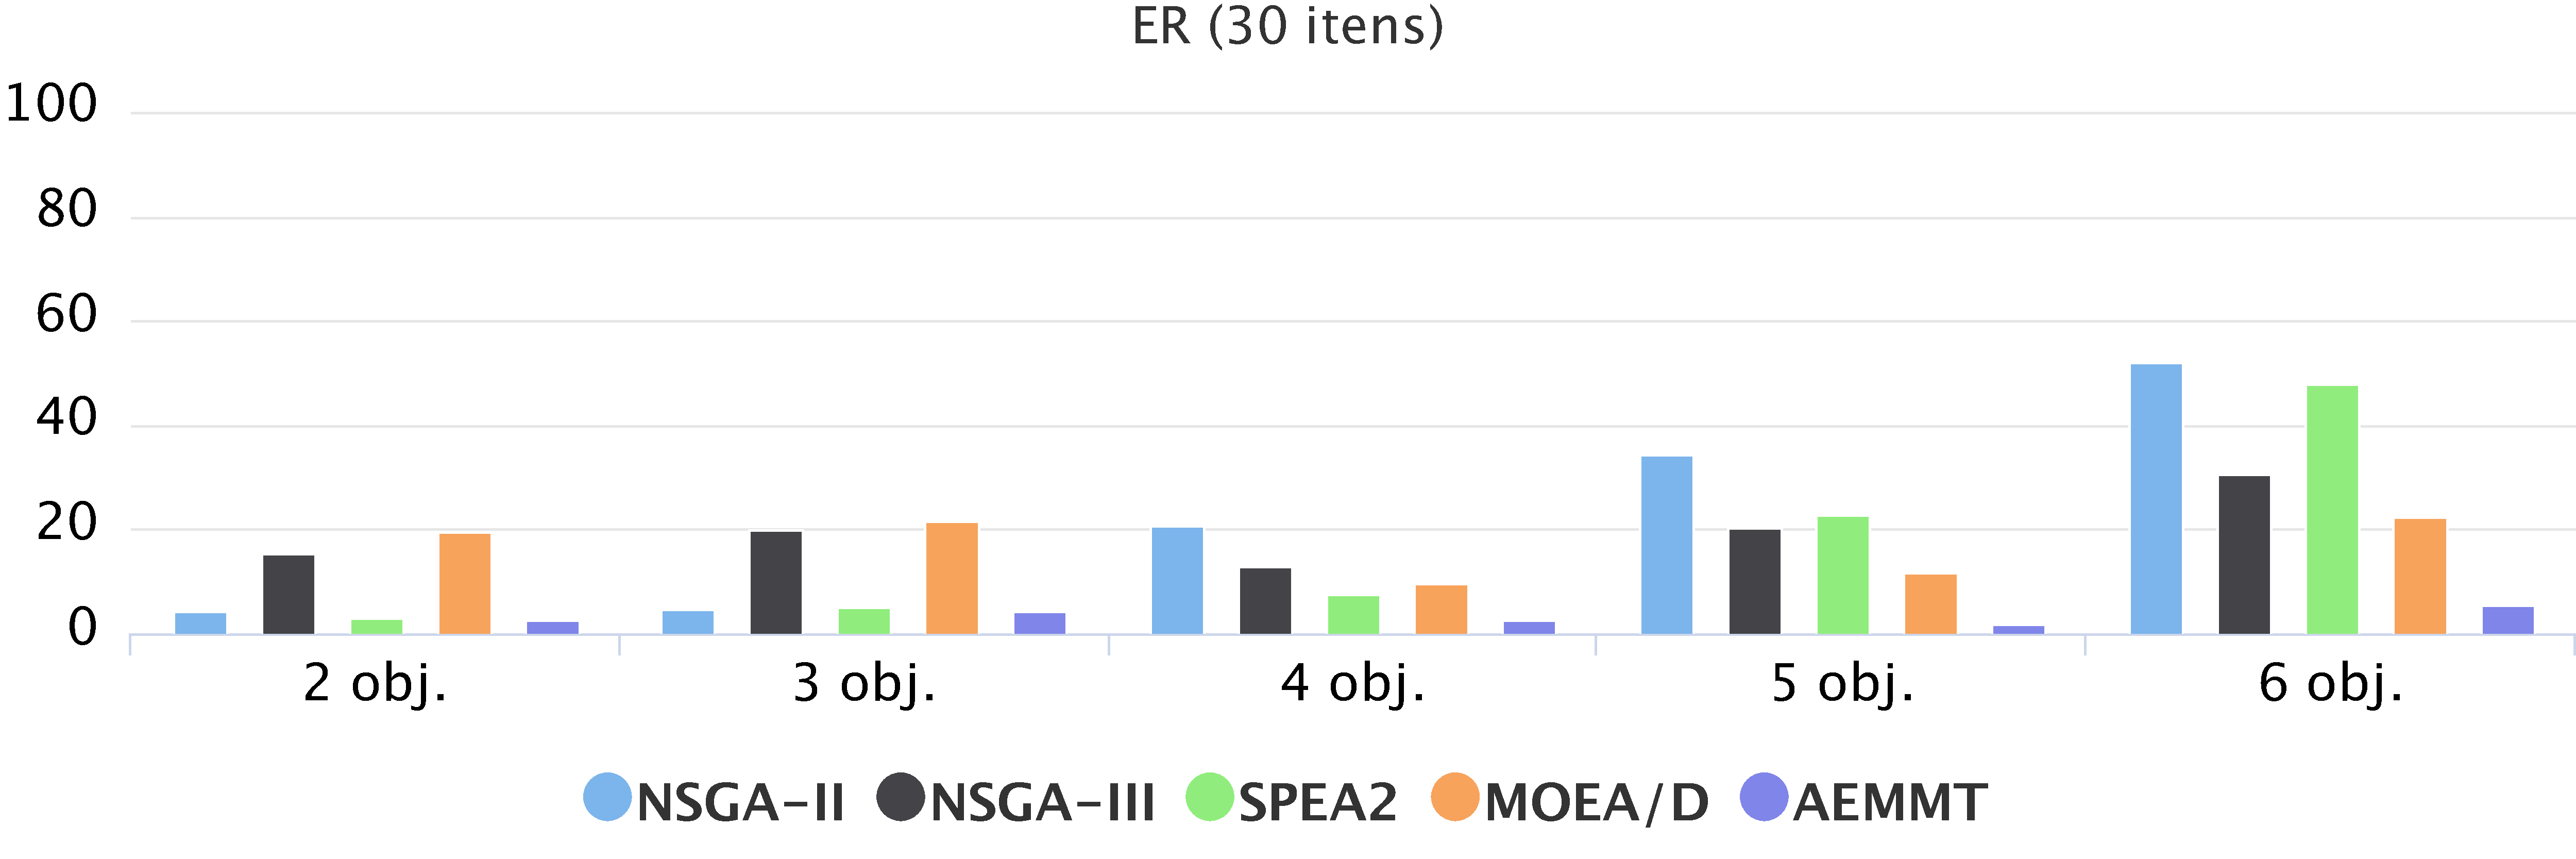
\includegraphics[width=1\textwidth]{cap_experimentos/figs/etapa1/er-mkp-30}
	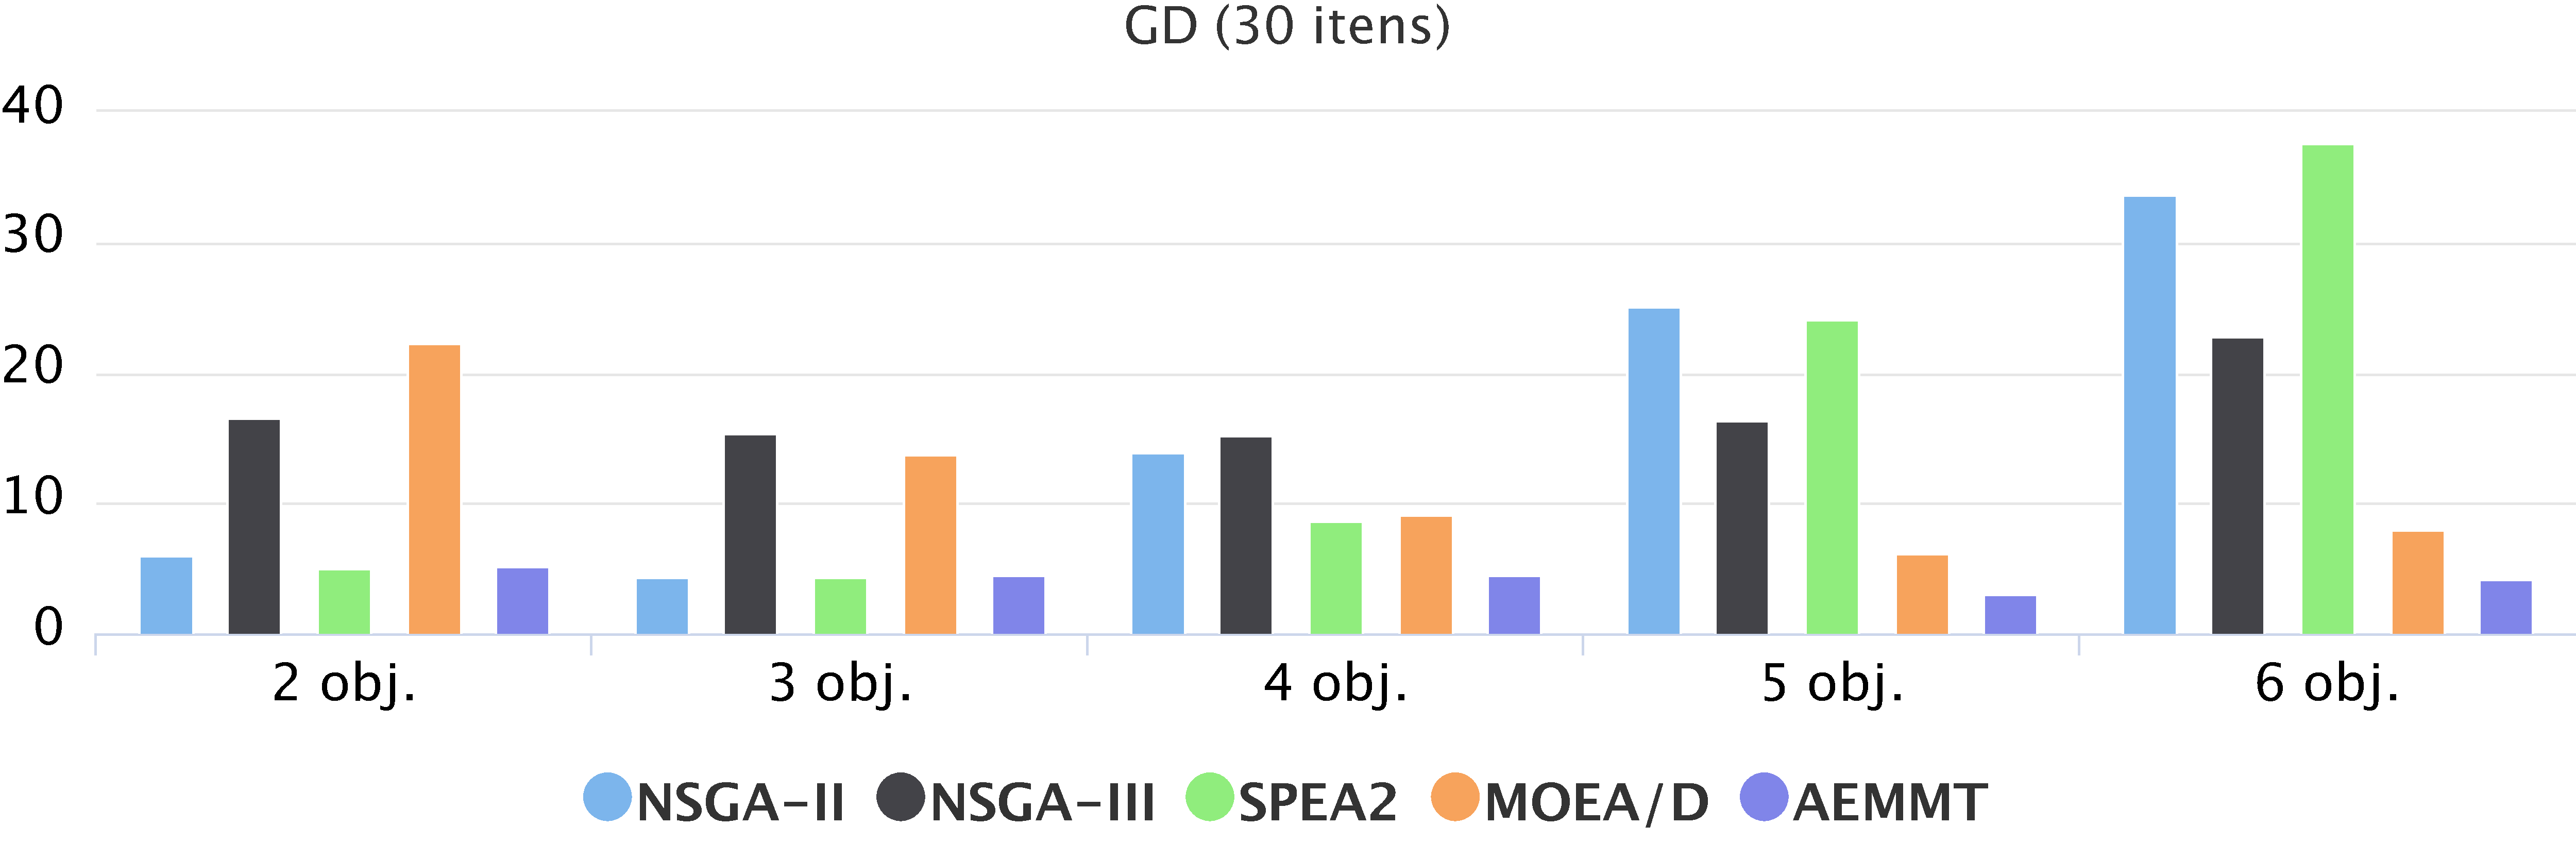
\includegraphics[width=1\textwidth]{cap_experimentos/figs/etapa1/gd-mkp-30}
	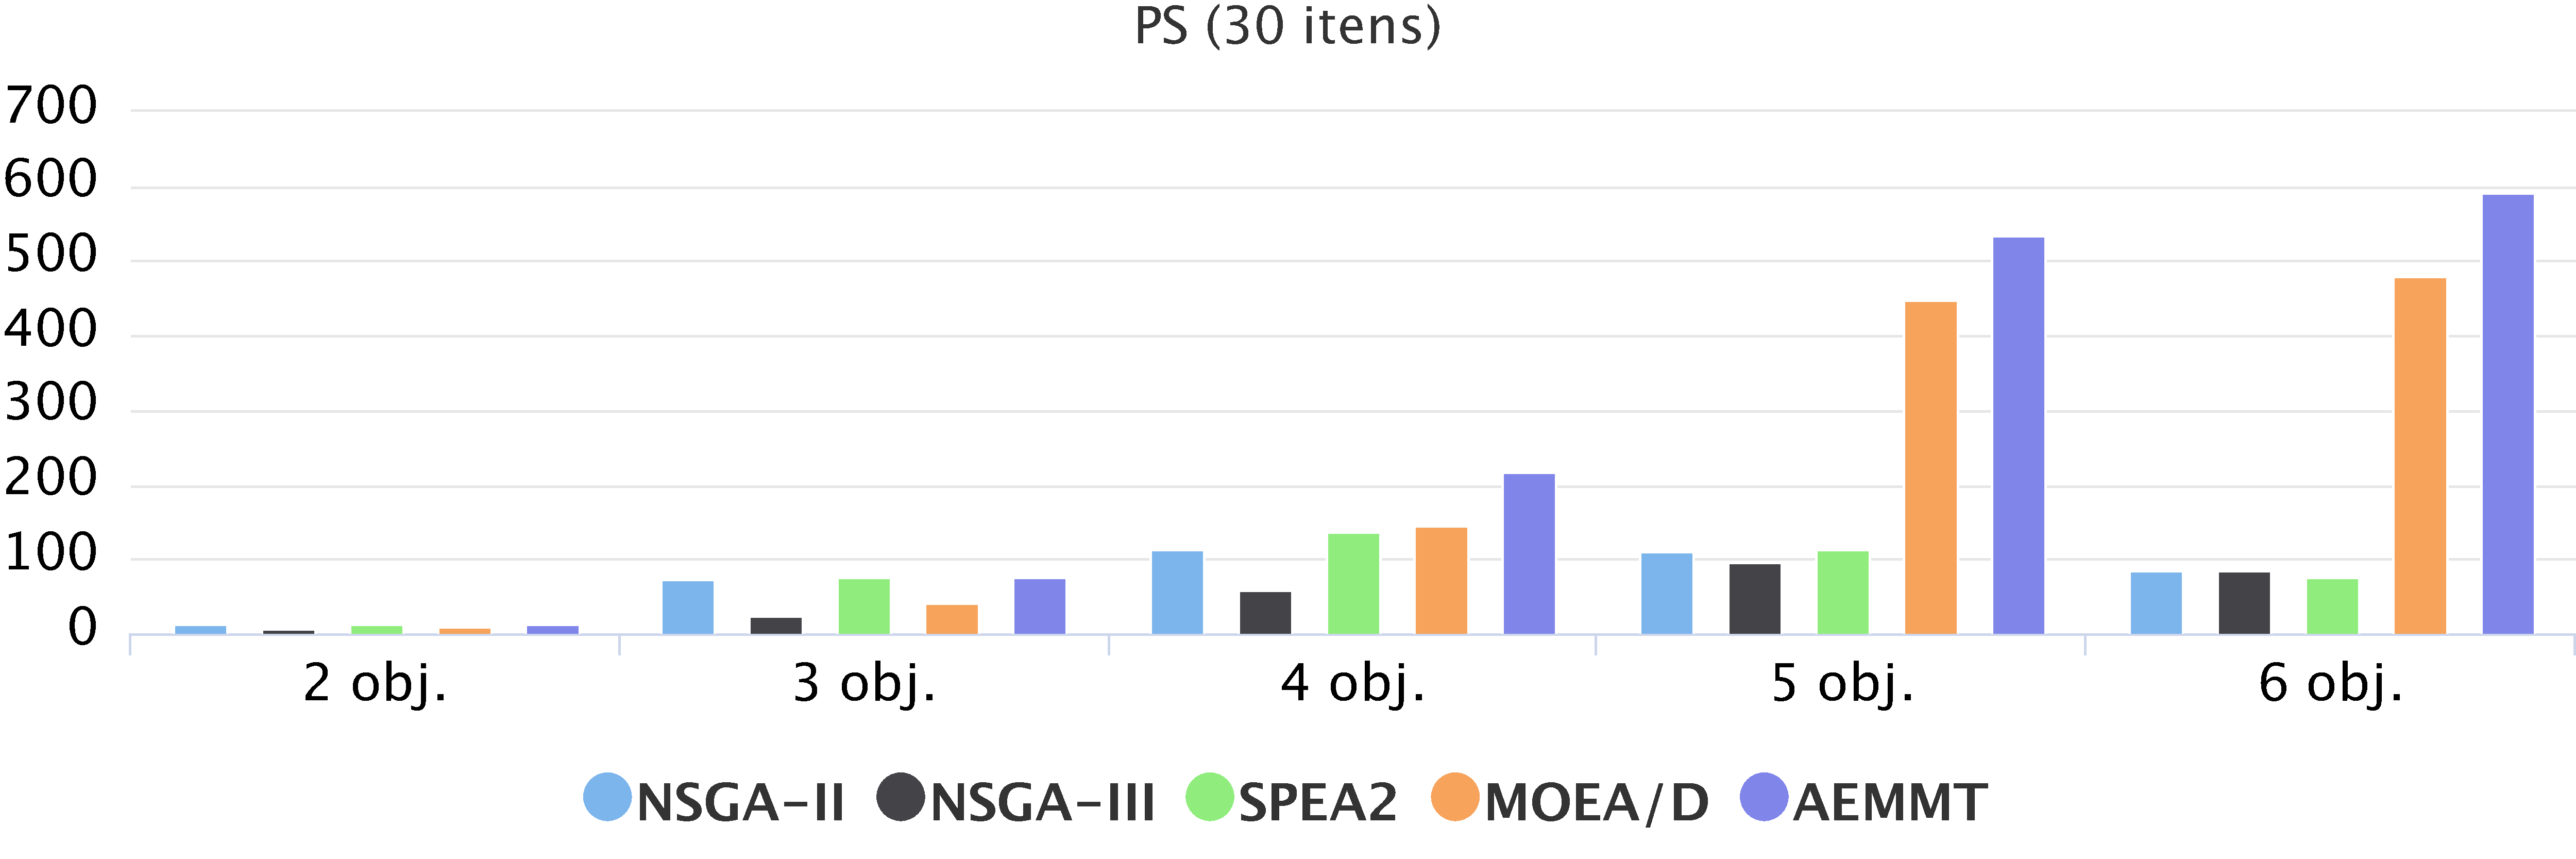
\includegraphics[width=1\textwidth]{cap_experimentos/figs/etapa1/ps-mkp-30}
\end{figure*}

O PMM com 30 itens (figura \ref{fig_exp1_pmm_30}) é um problema simples e geralmente qualquer método de otimização multiobjetivo atinge bons resultados. Até 4 objetivos, apenas o MOEA/D passou a marca de 20\% de erro. Para 2 e 3 objetivos, o NSGA-II, o SPEA2 e o AEMMT são indistinguíveis e possuem erro muito baixo. A partir de 4 objetivos é possível notar uma piora considerável nos algoritmos clássicos NSGA-II e SPEA-2. Considerando todas as formulações de objetivo, os melhores resultados foram obtidos pelo AEMMT que manteve o erro abaixo de 6\% em todos os casos. O $GD$ acompanha as conclusões tiradas a partir do $ER$, o AEMMT gera, globalmente, os melhores resultados enquanto, apesar de terem ótimo desempenho nos problemas de 2 e 3 objetivos, o NSGA-II e o SPEA2 sofrem a partir de 4 objetivos. O tamanho da fronteira de Pareto encontrada, medida pelo $PS$, é maior nos algoritmos MOEA/D e AEMMT, o que é esperado, pois diferentemente dos demais, esses dois algoritmos não aplicam uma limitação muito grande sobre o tamanho do Pareto. Para o PMM de 30 itens está claro que, em qualquer situação, o AEMMT é o melhor dentre os métodos testados.

\begin{figure*}[!htbp]
	\caption{Etapa 1: resultados para o PMM com 50 itens}
	\label{fig_exp1_pmm_50}
	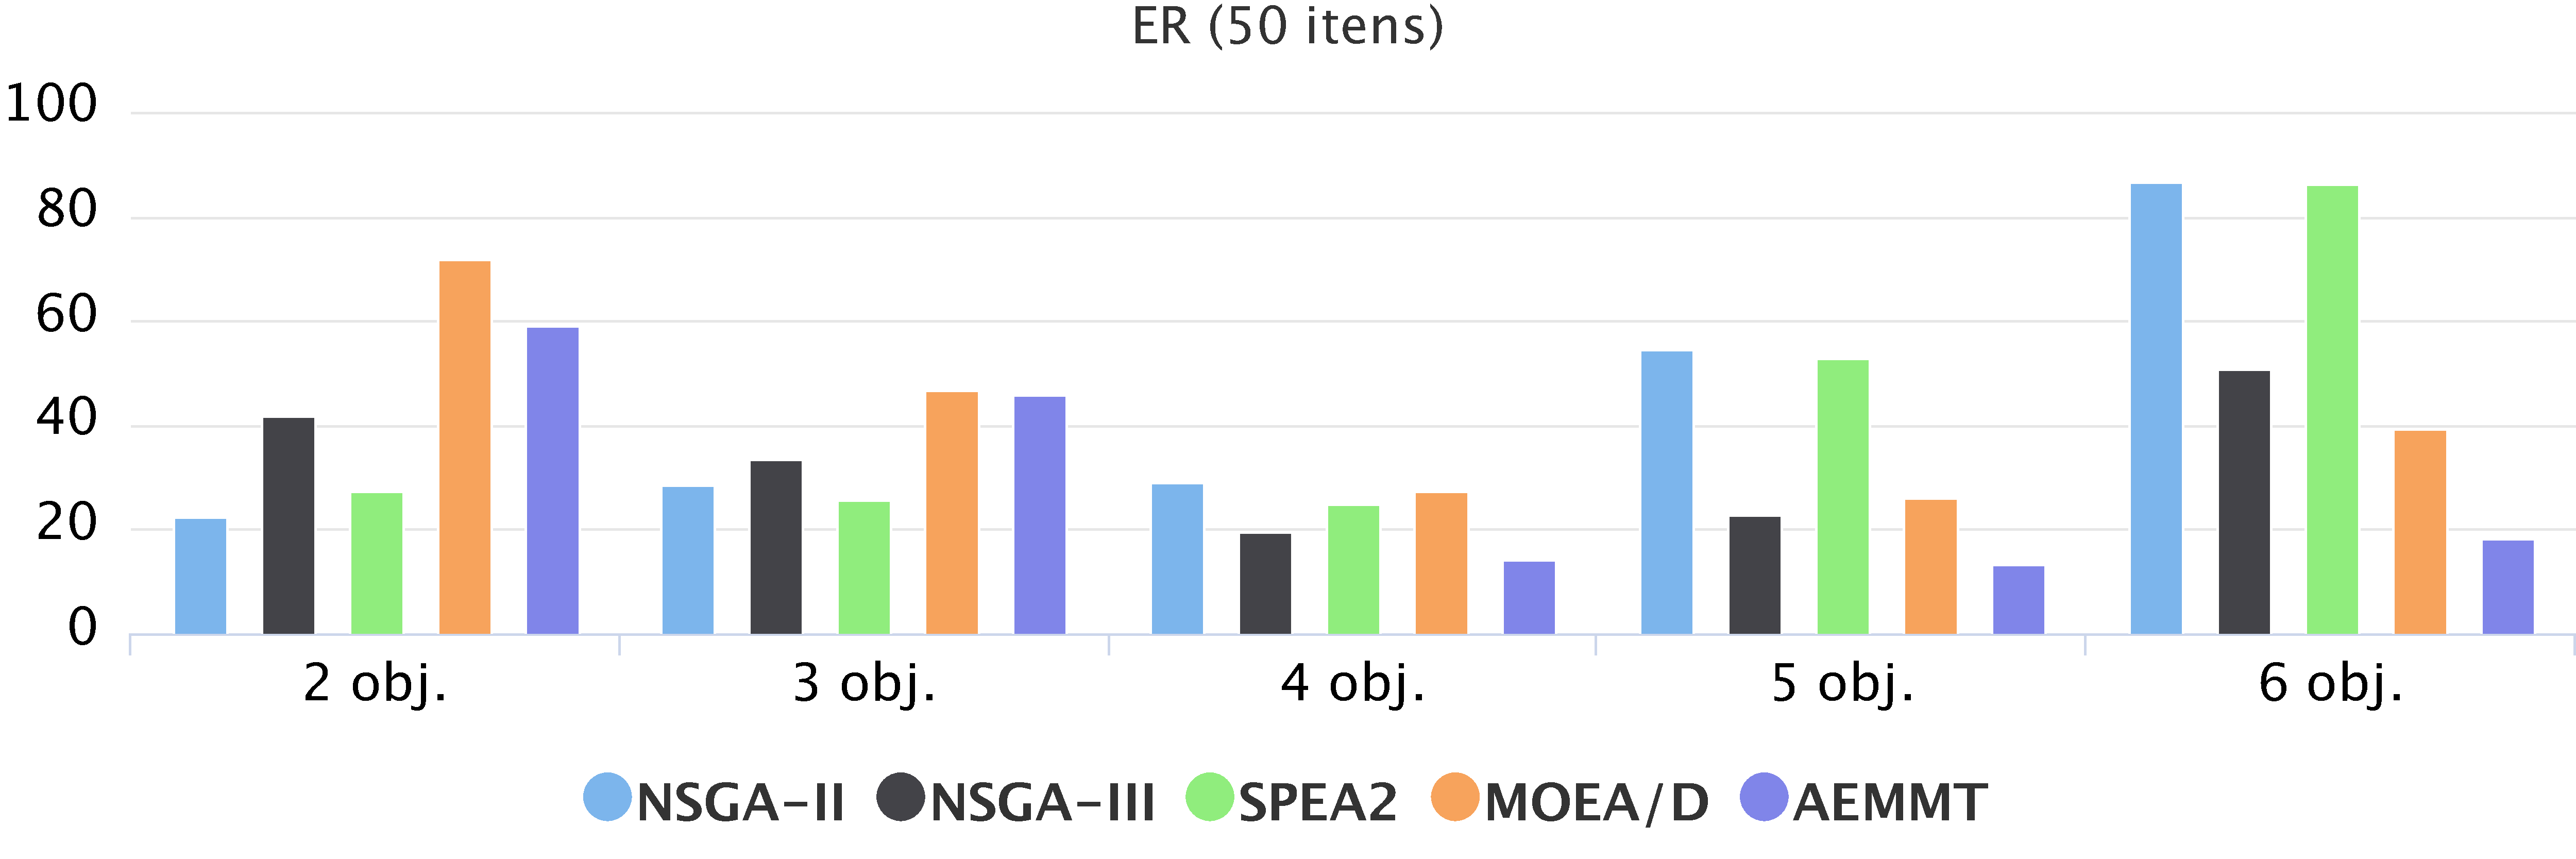
\includegraphics[width=1\textwidth]{cap_experimentos/figs/etapa1/er-mkp-50}
	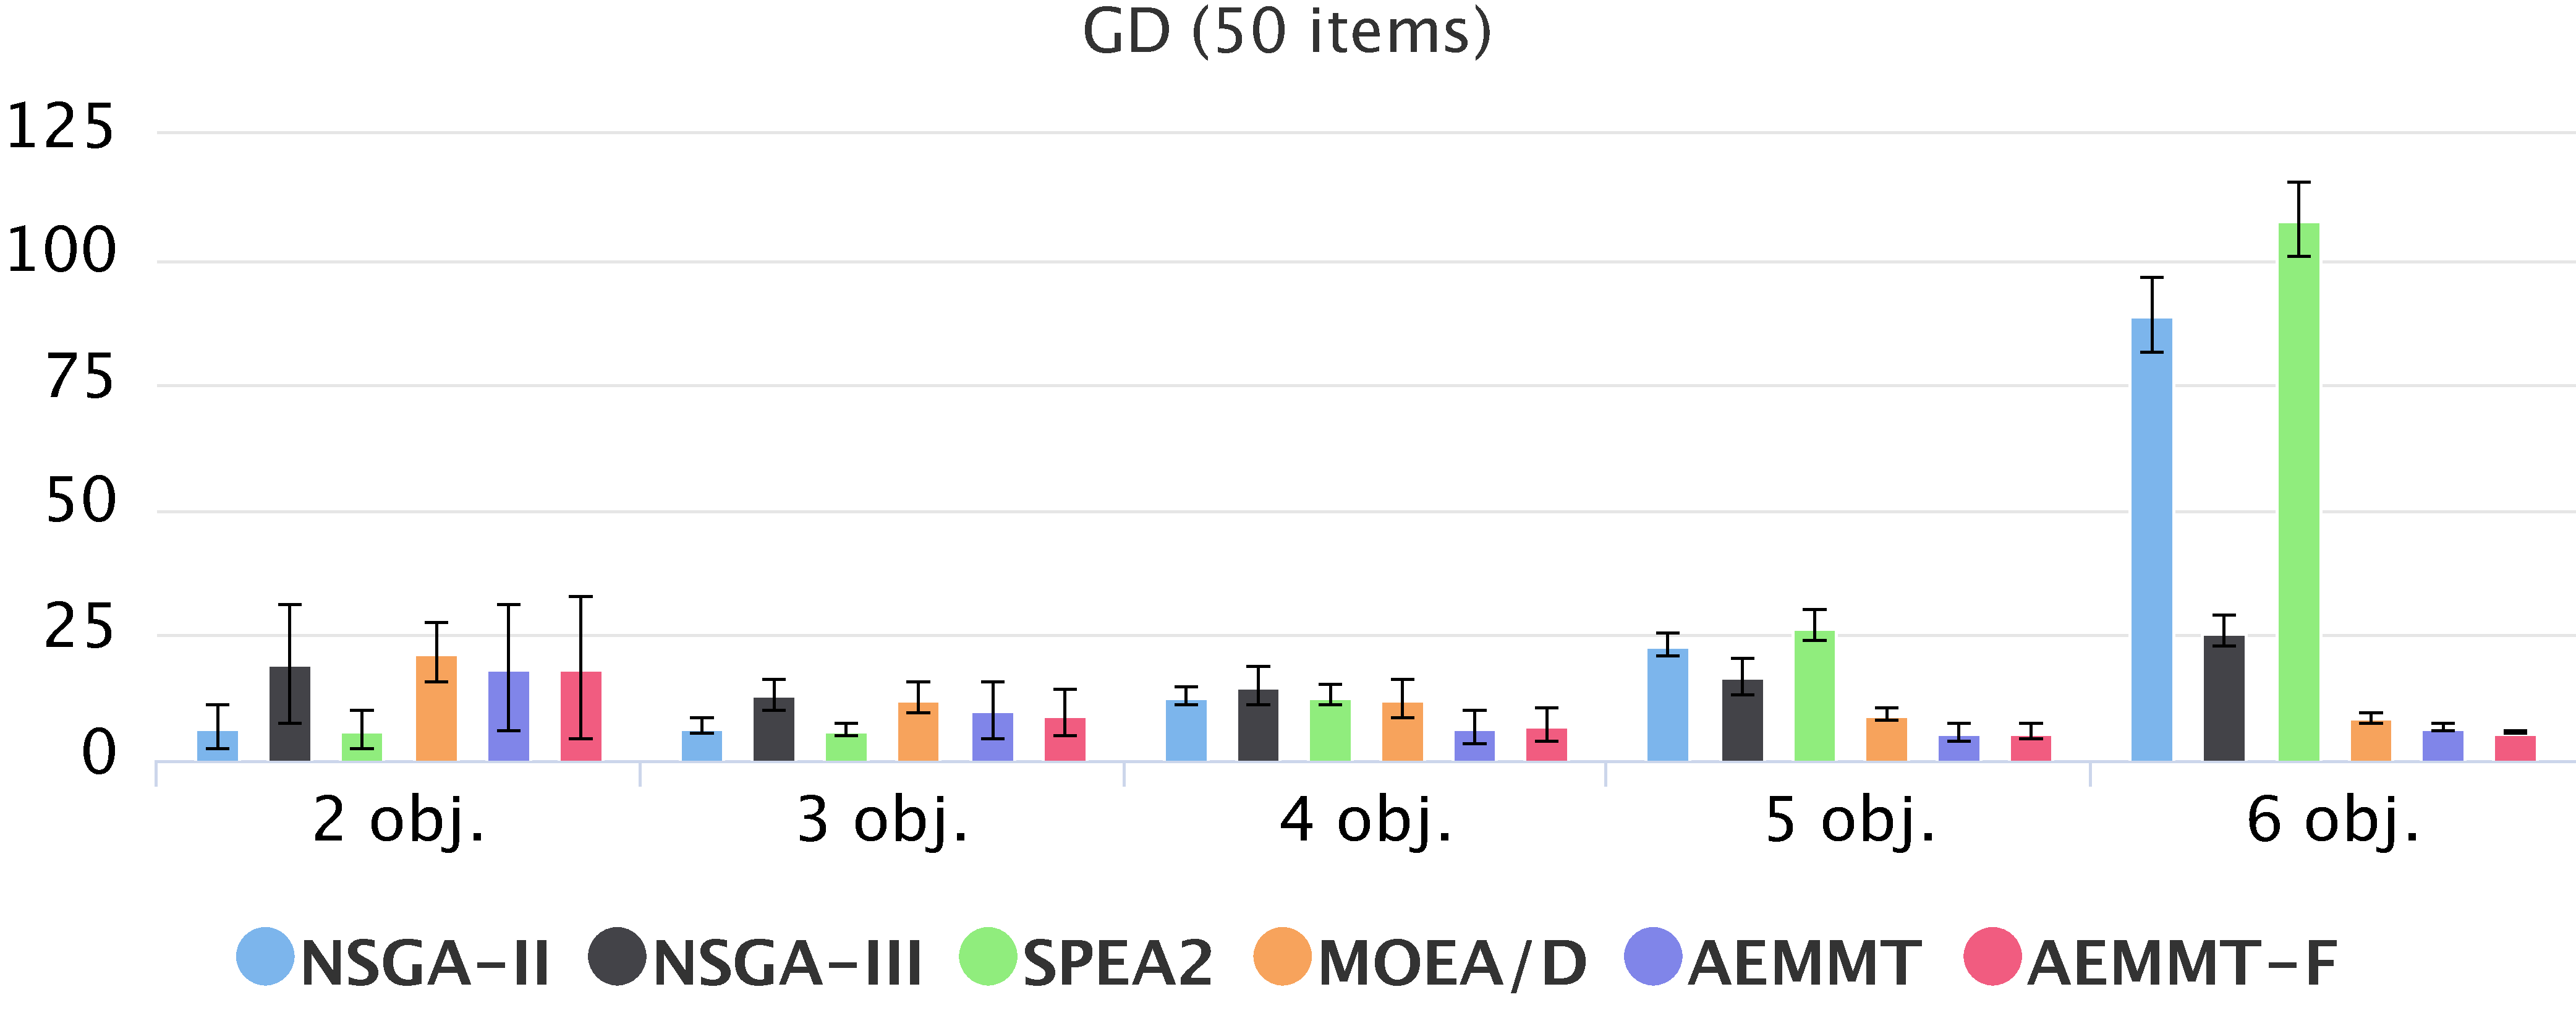
\includegraphics[width=1\textwidth]{cap_experimentos/figs/etapa1/gd-mkp-50}
	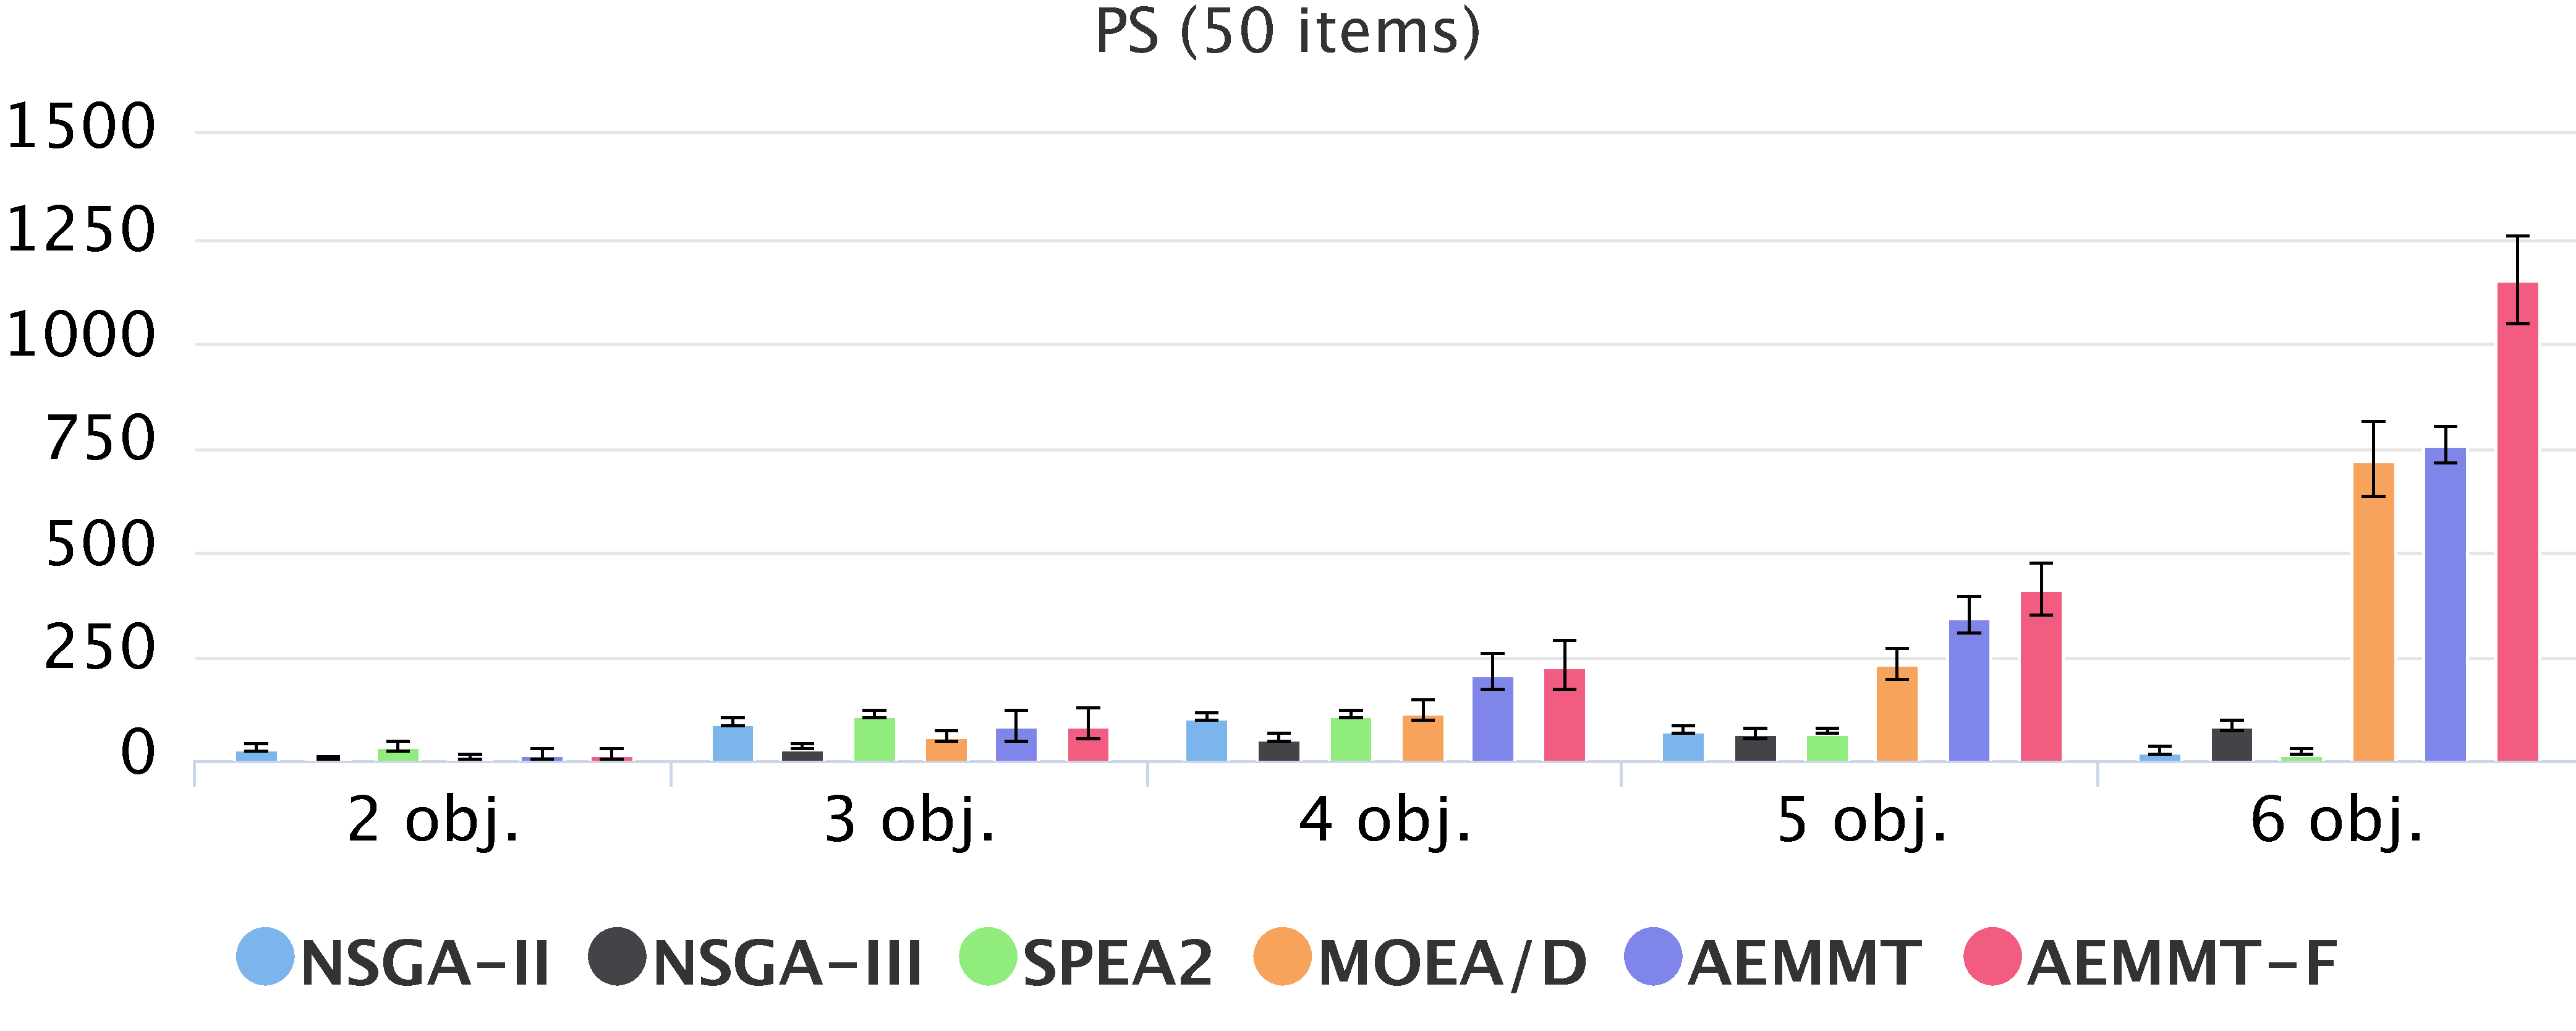
\includegraphics[width=1\textwidth]{cap_experimentos/figs/etapa1/ps-mkp-50}
\end{figure*}

O PMM com 50 itens (figura \ref{fig_exp1_pmm_50}) é um problema bem mais complexo que o PMM de 30 itens e já permite visualizar bem o comportamento de cada algoritmo nos diferentes cenários. Considerando as três métricas ($ER$, $GD$ e $PS$) os algoritmos clássicos (NSGA-II e SPEA2) são imbatíveis nas formulações com 2 e 3 objetivos. A partir de 4 objetivos a situação muda e o AEMMT passa a apresentar melhores resultados, ao aumentar os objetivos, o NSGA-II e o SPEA2 pioram enquanto o AEMMT mantém o $ER$ e o $GD$ estáveis e melhora o $PS$. O MOEA/D é o segundo melhor algoritmo para problemas \textit{many-objectives} e o NSGA-III é o terceiro. Para o PMM de 50 itens, o AEMMT é claramente a melhor opção.

\begin{figure*}[!htbp]
	\caption{Etapa 1: resultados para o PMM com 100 itens}
	\label{fig_exp1_pmm_100}
	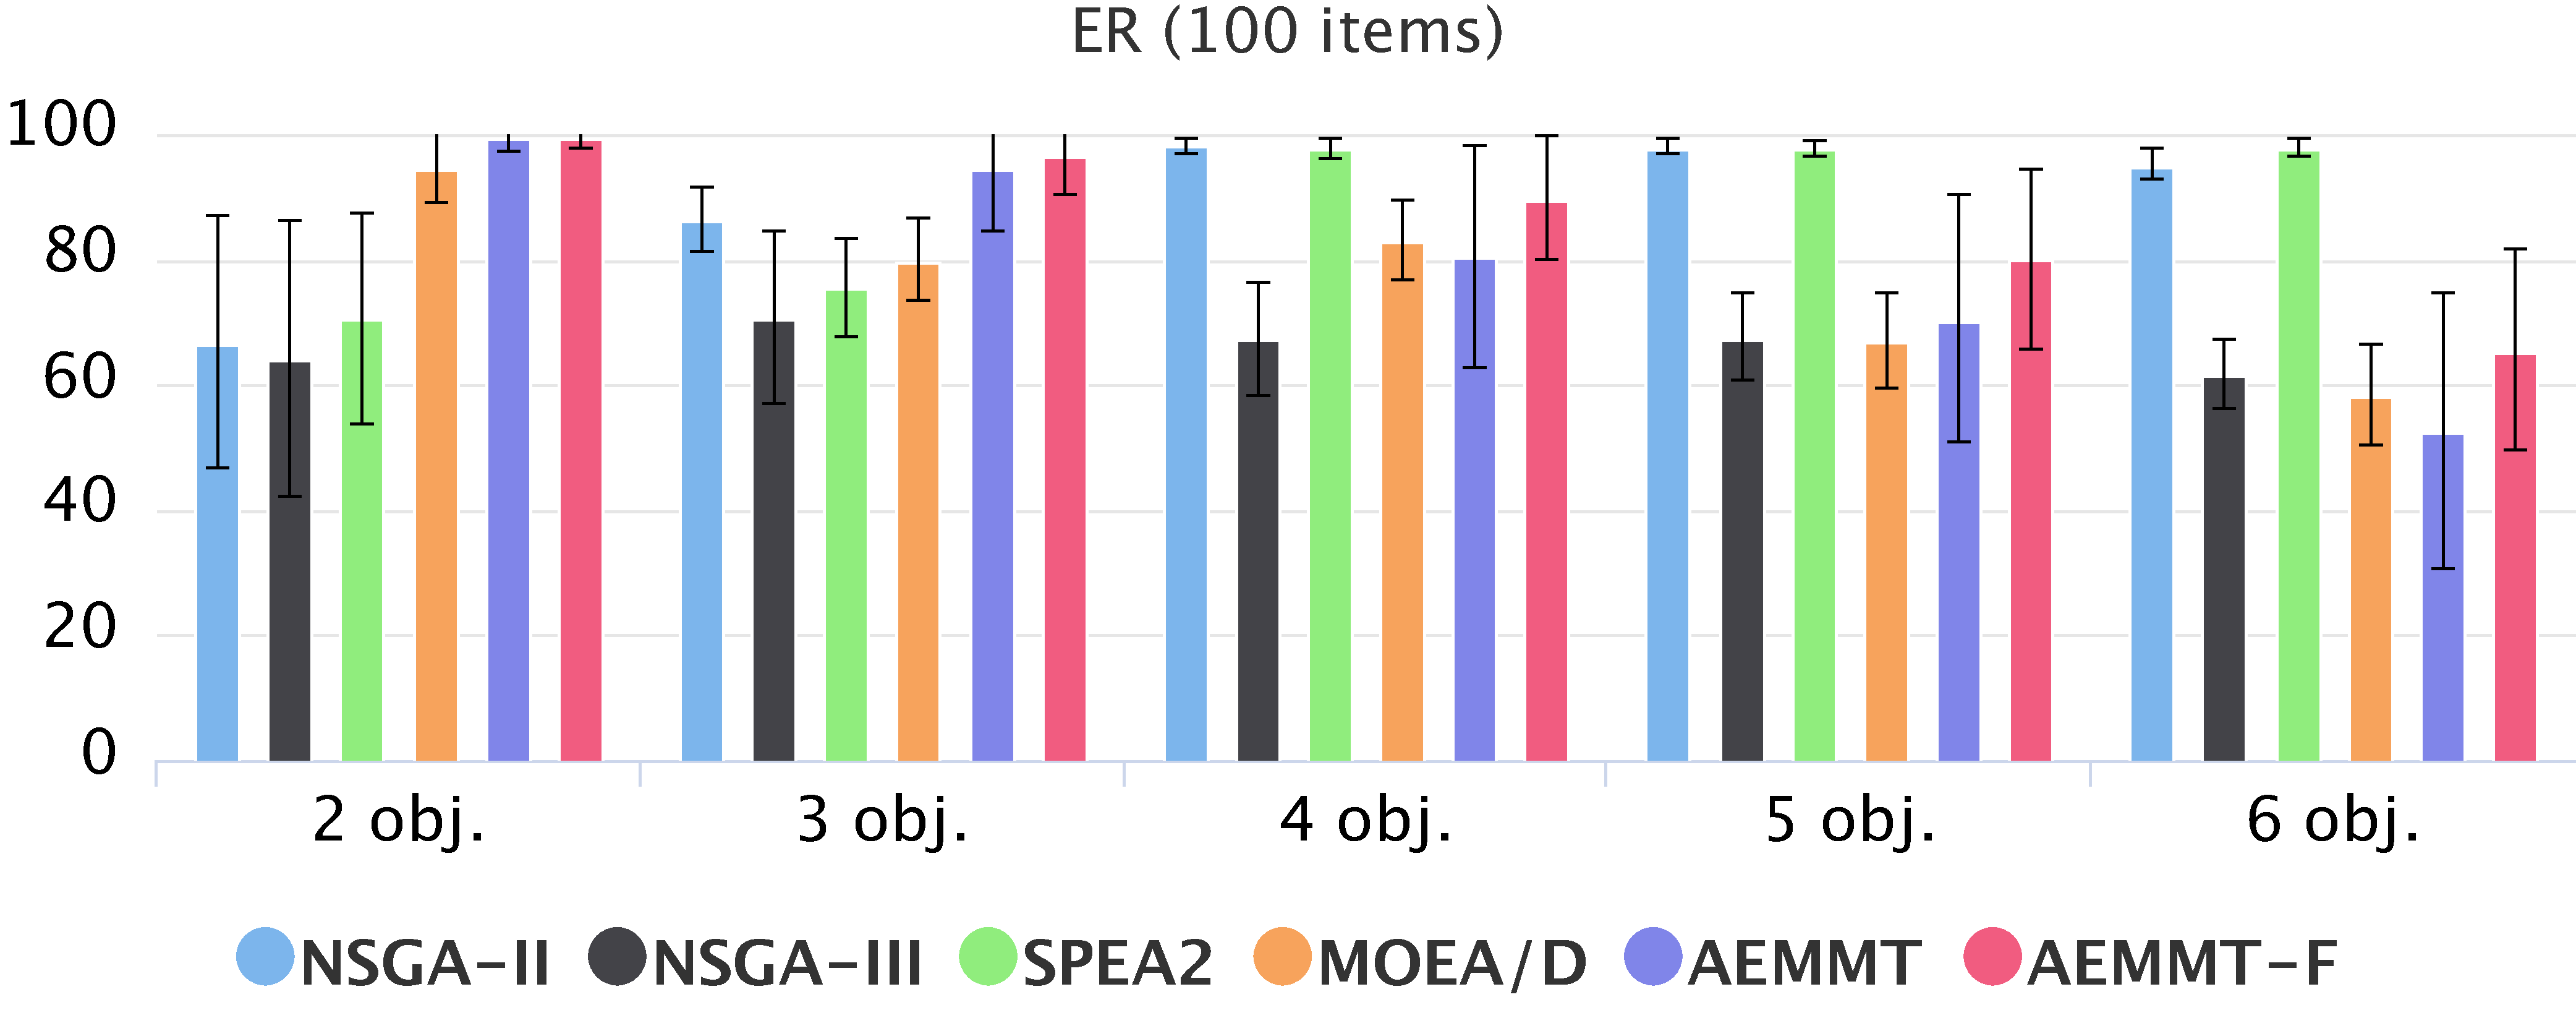
\includegraphics[width=1\textwidth]{cap_experimentos/figs/etapa1/er-mkp-100}
	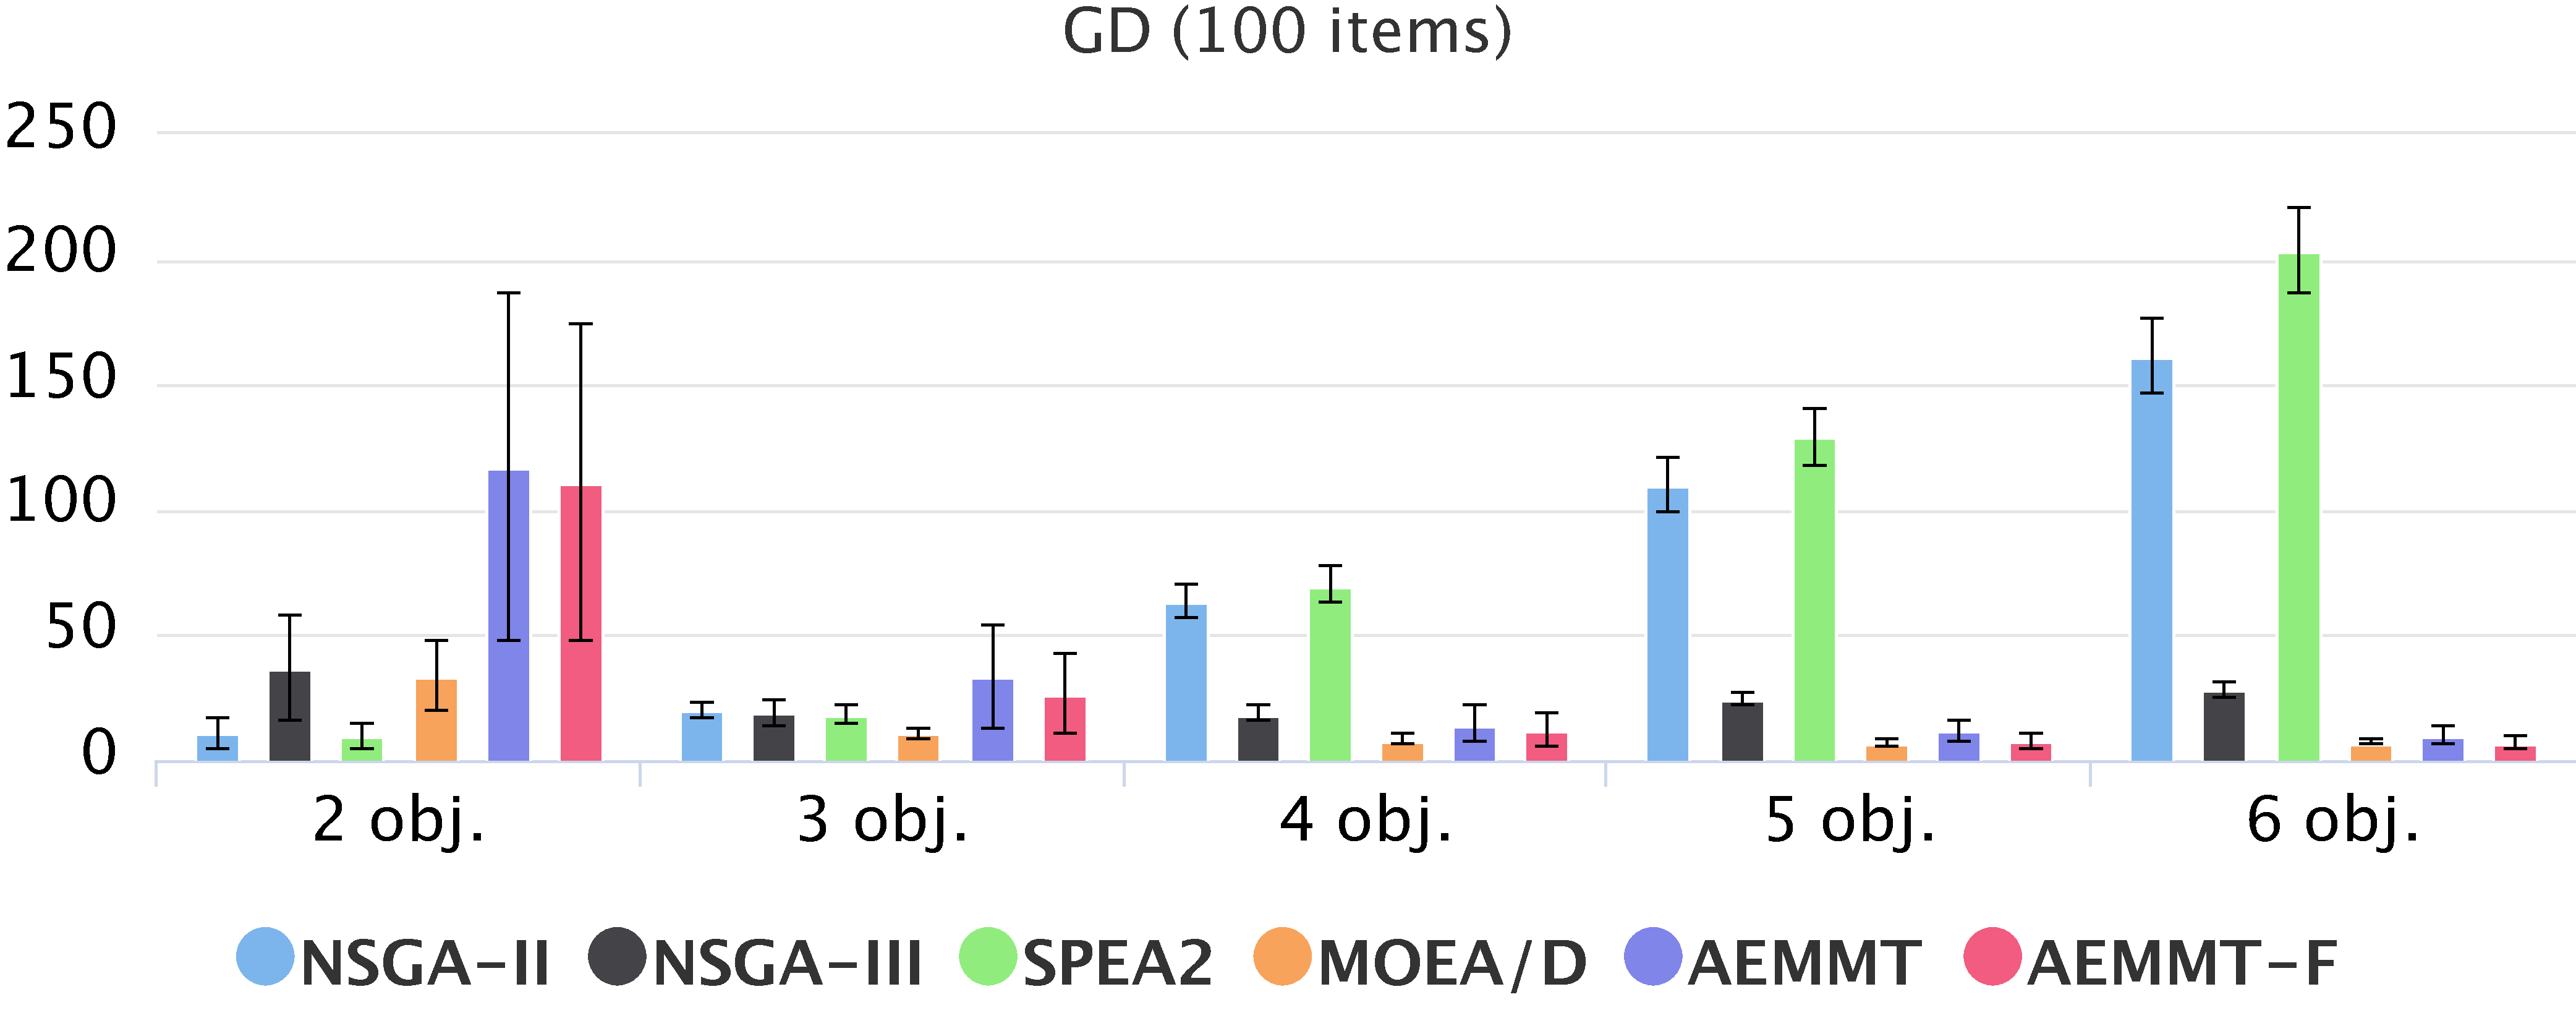
\includegraphics[width=1\textwidth]{cap_experimentos/figs/etapa1/gd-mkp-100}
	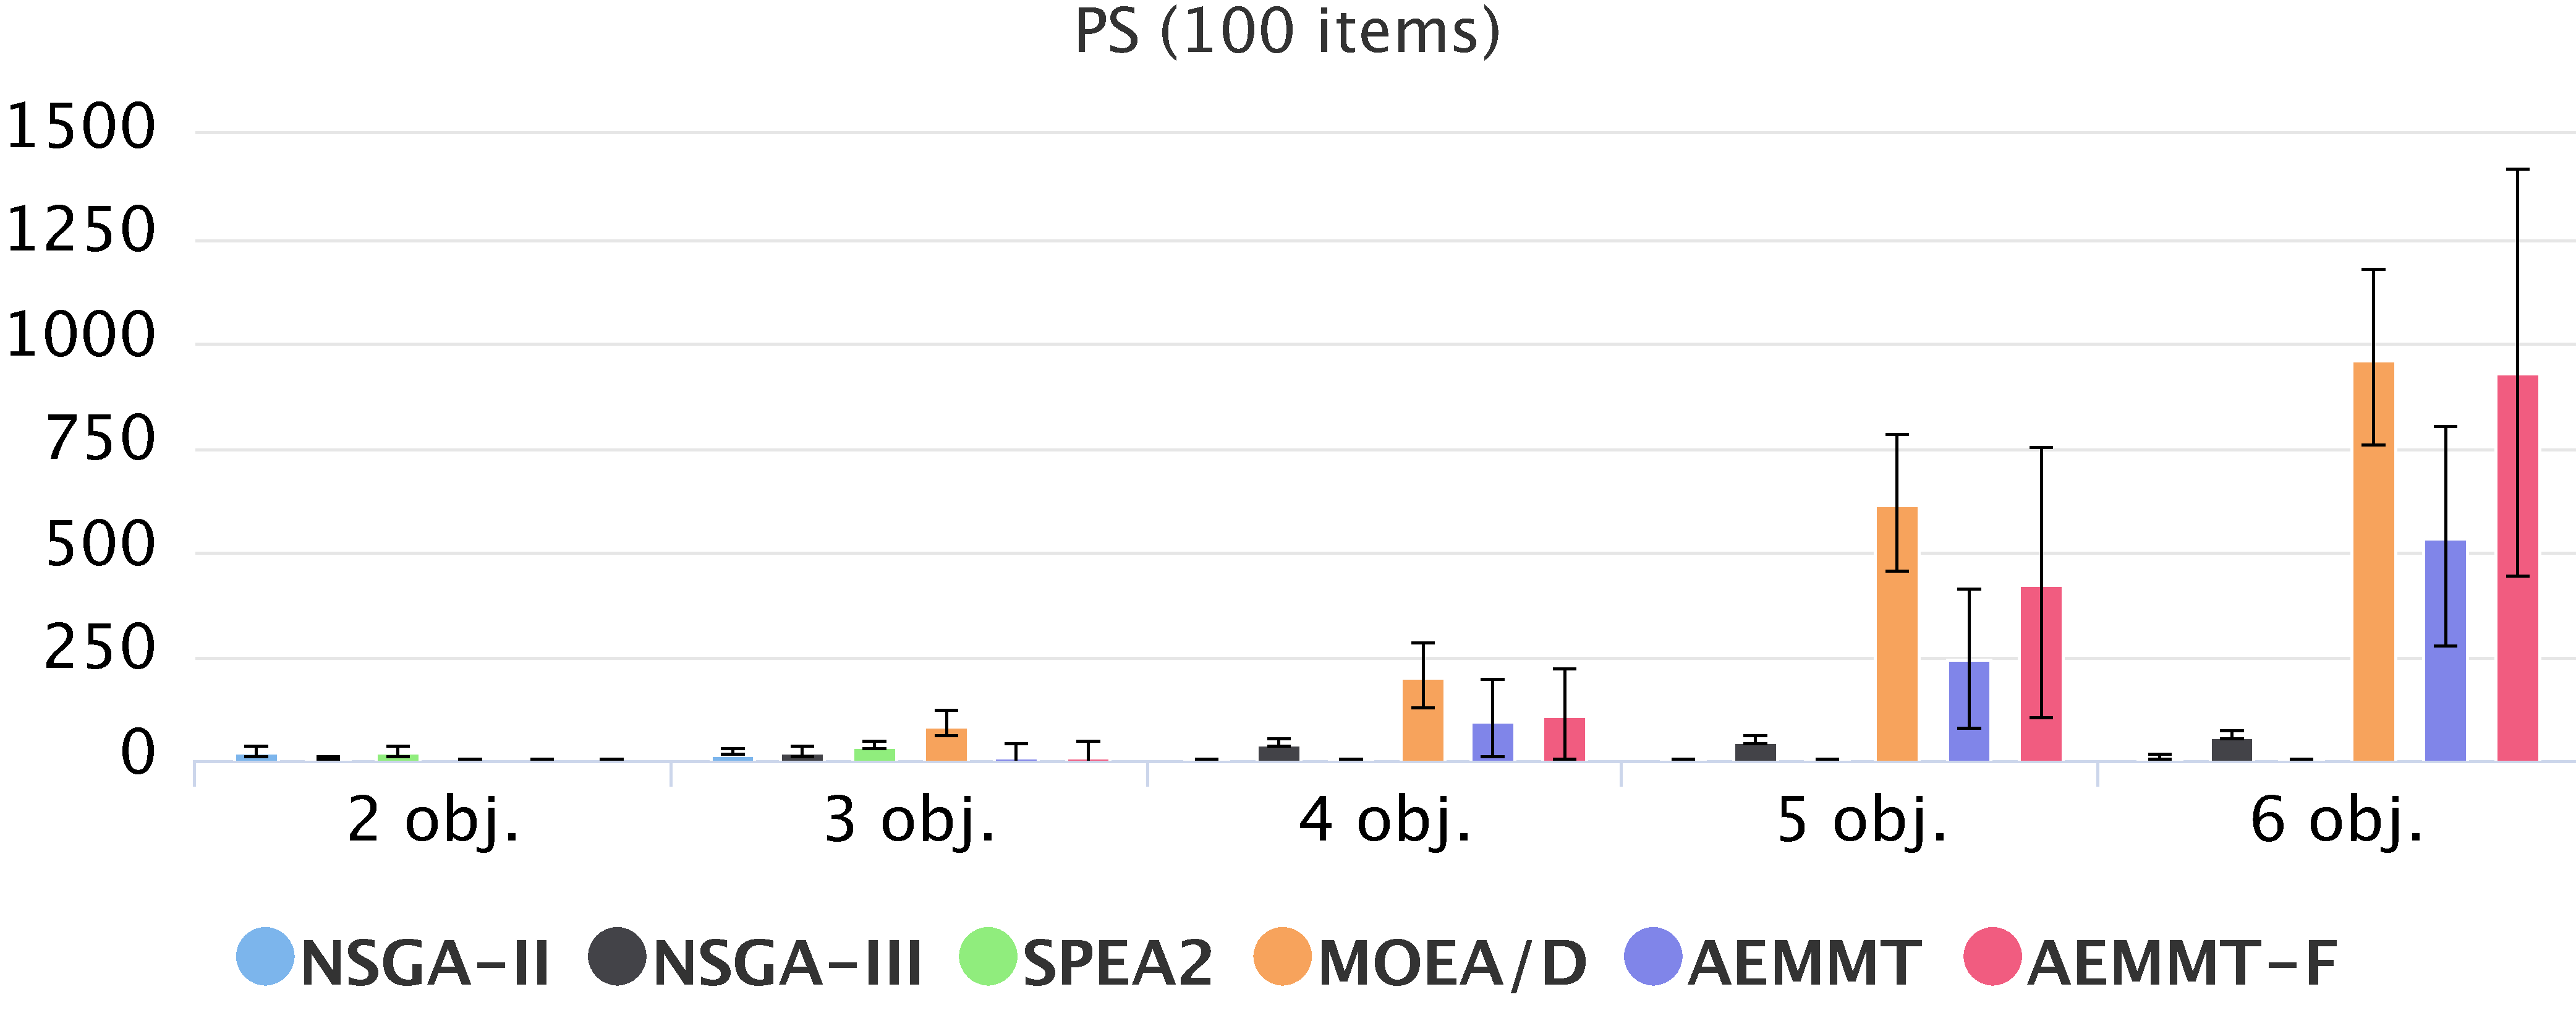
\includegraphics[width=1\textwidth]{cap_experimentos/figs/etapa1/ps-mkp-100}
\end{figure*}

O tamanho do espaço de busca no problema da mochila pode ser medido através da equação $2^n$, onde $n$ é o número de itens. Portanto, a complexidade do PMM com 100 itens (figura \ref{fig_exp1_pmm_100}) é absurdamente maior que os anteriores. Por essa razão, não foi possível encontrar um Pareto estável para as formulações de 4, 5 e 6 objetivos. Dessa forma, apesar de as métricas $ER$, $GD$ e $PS$ serem um bom indicativo da performance entre os algoritmos, a melhor forma de avaliação seria o hiper-volume. Um experimento parecido com este, mas utilizando o hiper-volume é apresentado na seção \ref{section_experimentos_etapa4}. É difícil avaliar o problema de 100 itens, pois, já no erro é possível perceber que poucos algoritmos conseguiram encontrar boas soluções, a menor taxa de erro está acima de 50\%. No PMM de 100 itens o NSGA-III apresentou o menor $ER$ nos cenários de 2, 3, 4 e 5 objetivos, e na formulação de 6, foi ultrapassado pelos AEMMT e MOEA/D. Com relação ao $GD$, para 2 objetivos, o NSGA-II e o SPEA2 apresentaram os melhores resultados. Na formulação de 3 objetivos em diante, o MOEA/D foi o algoritmo com menor $GD$, sendo que em 4, 5 e 6 objetivos o AEMMT obteve desempenho similar. A situação se repete ao analisar o $PS$: a partir de 3 objetivos, o MOEA/D traz um conjunto maior de soluções na fronteira de Pareto, seguido pelo AEMMT a partir de 4 objetivos.

\begin{figure*}[!htbp]
	\caption{Etapa 1: resultados agrupados para o PMM com 30, 50 e 100 itens}
	\label{fig_exp1_pmm_todos}
	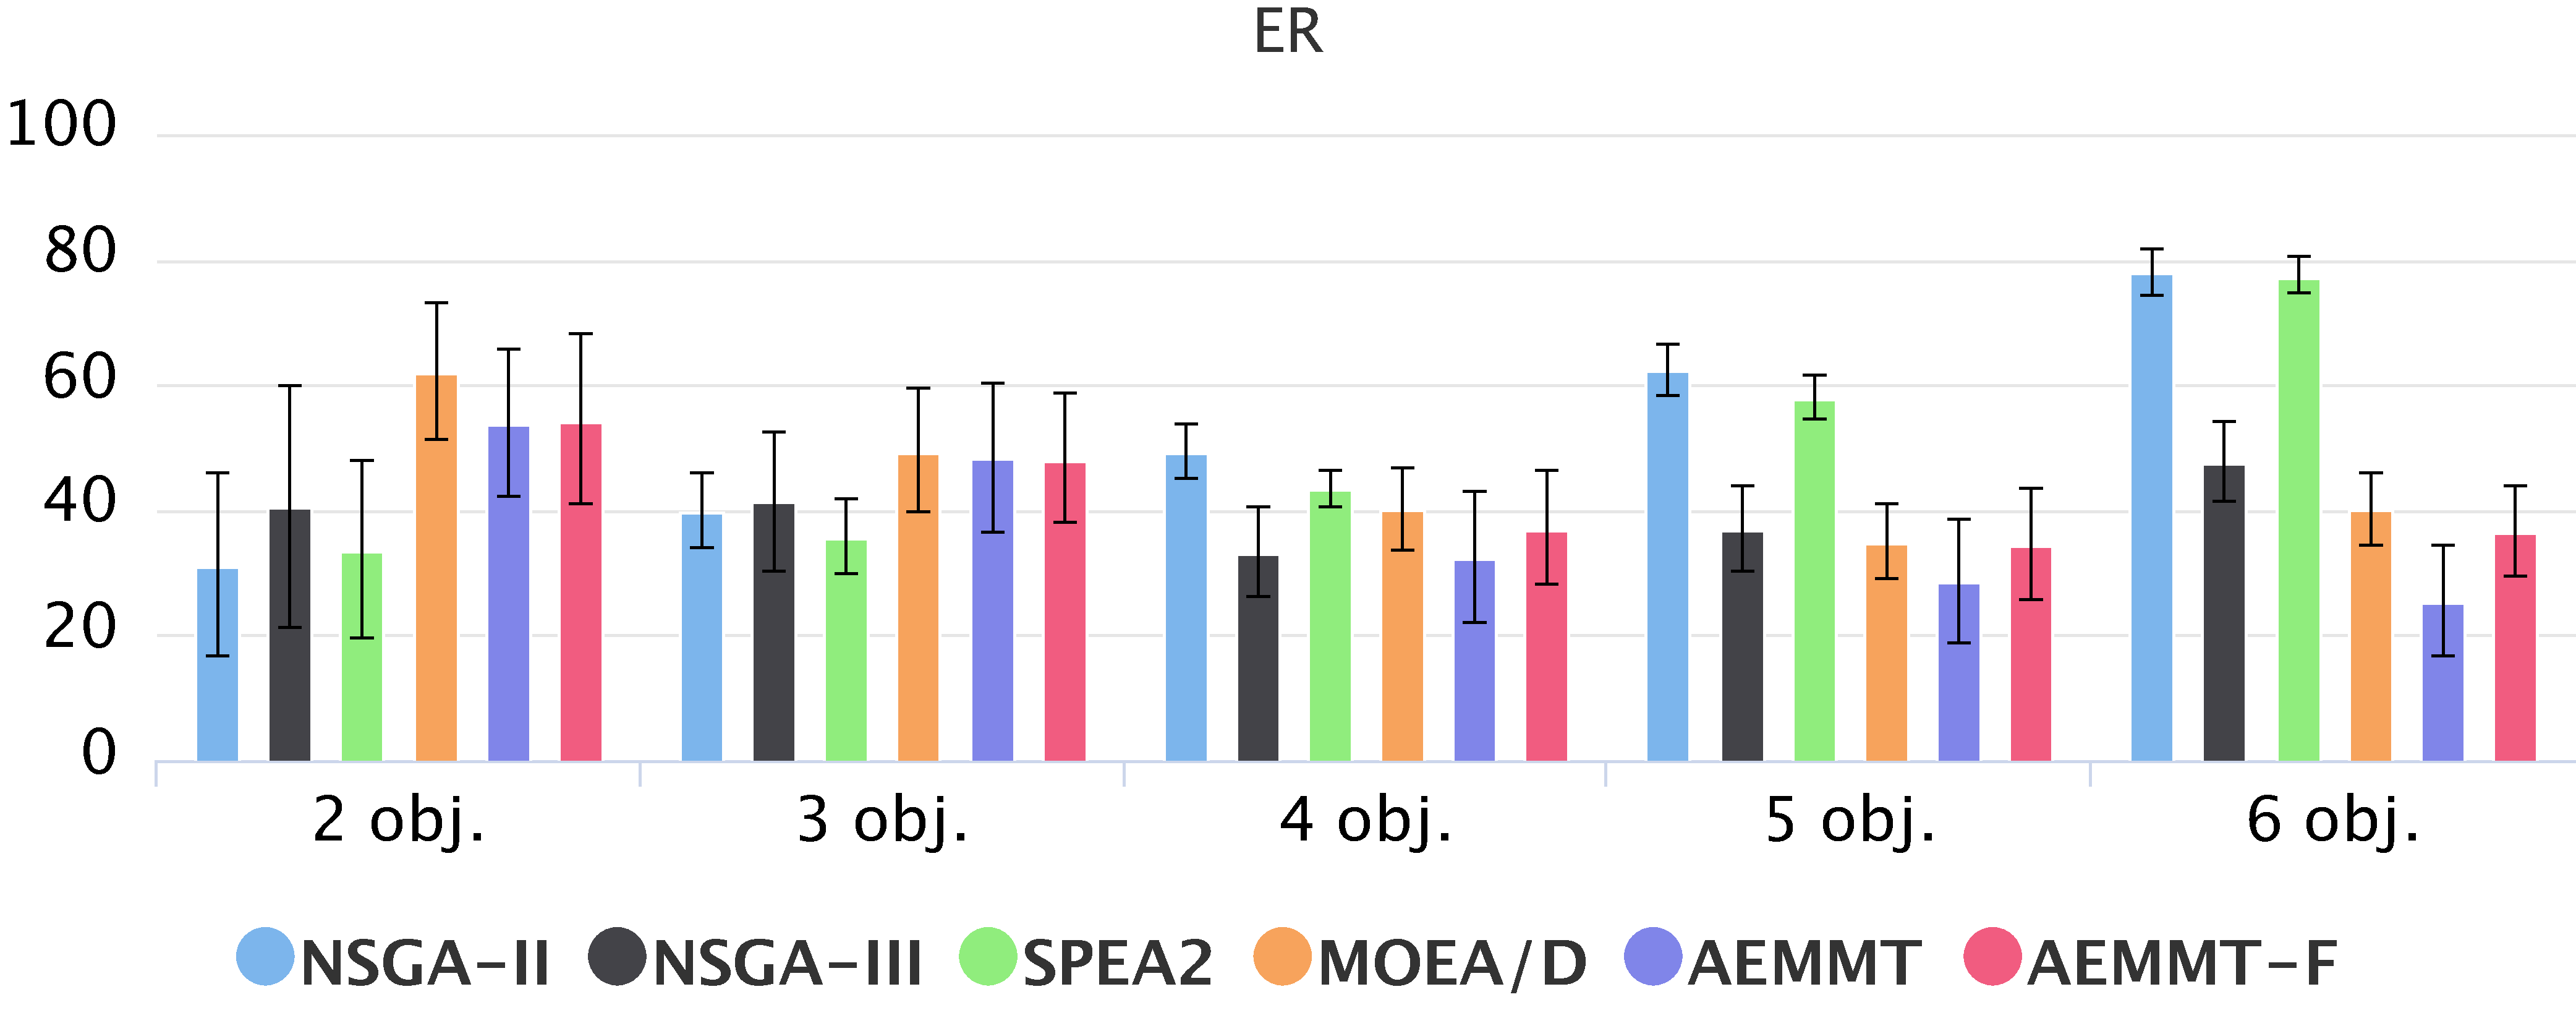
\includegraphics[width=1\textwidth]{cap_experimentos/figs/etapa1/er-mkp-todos}
	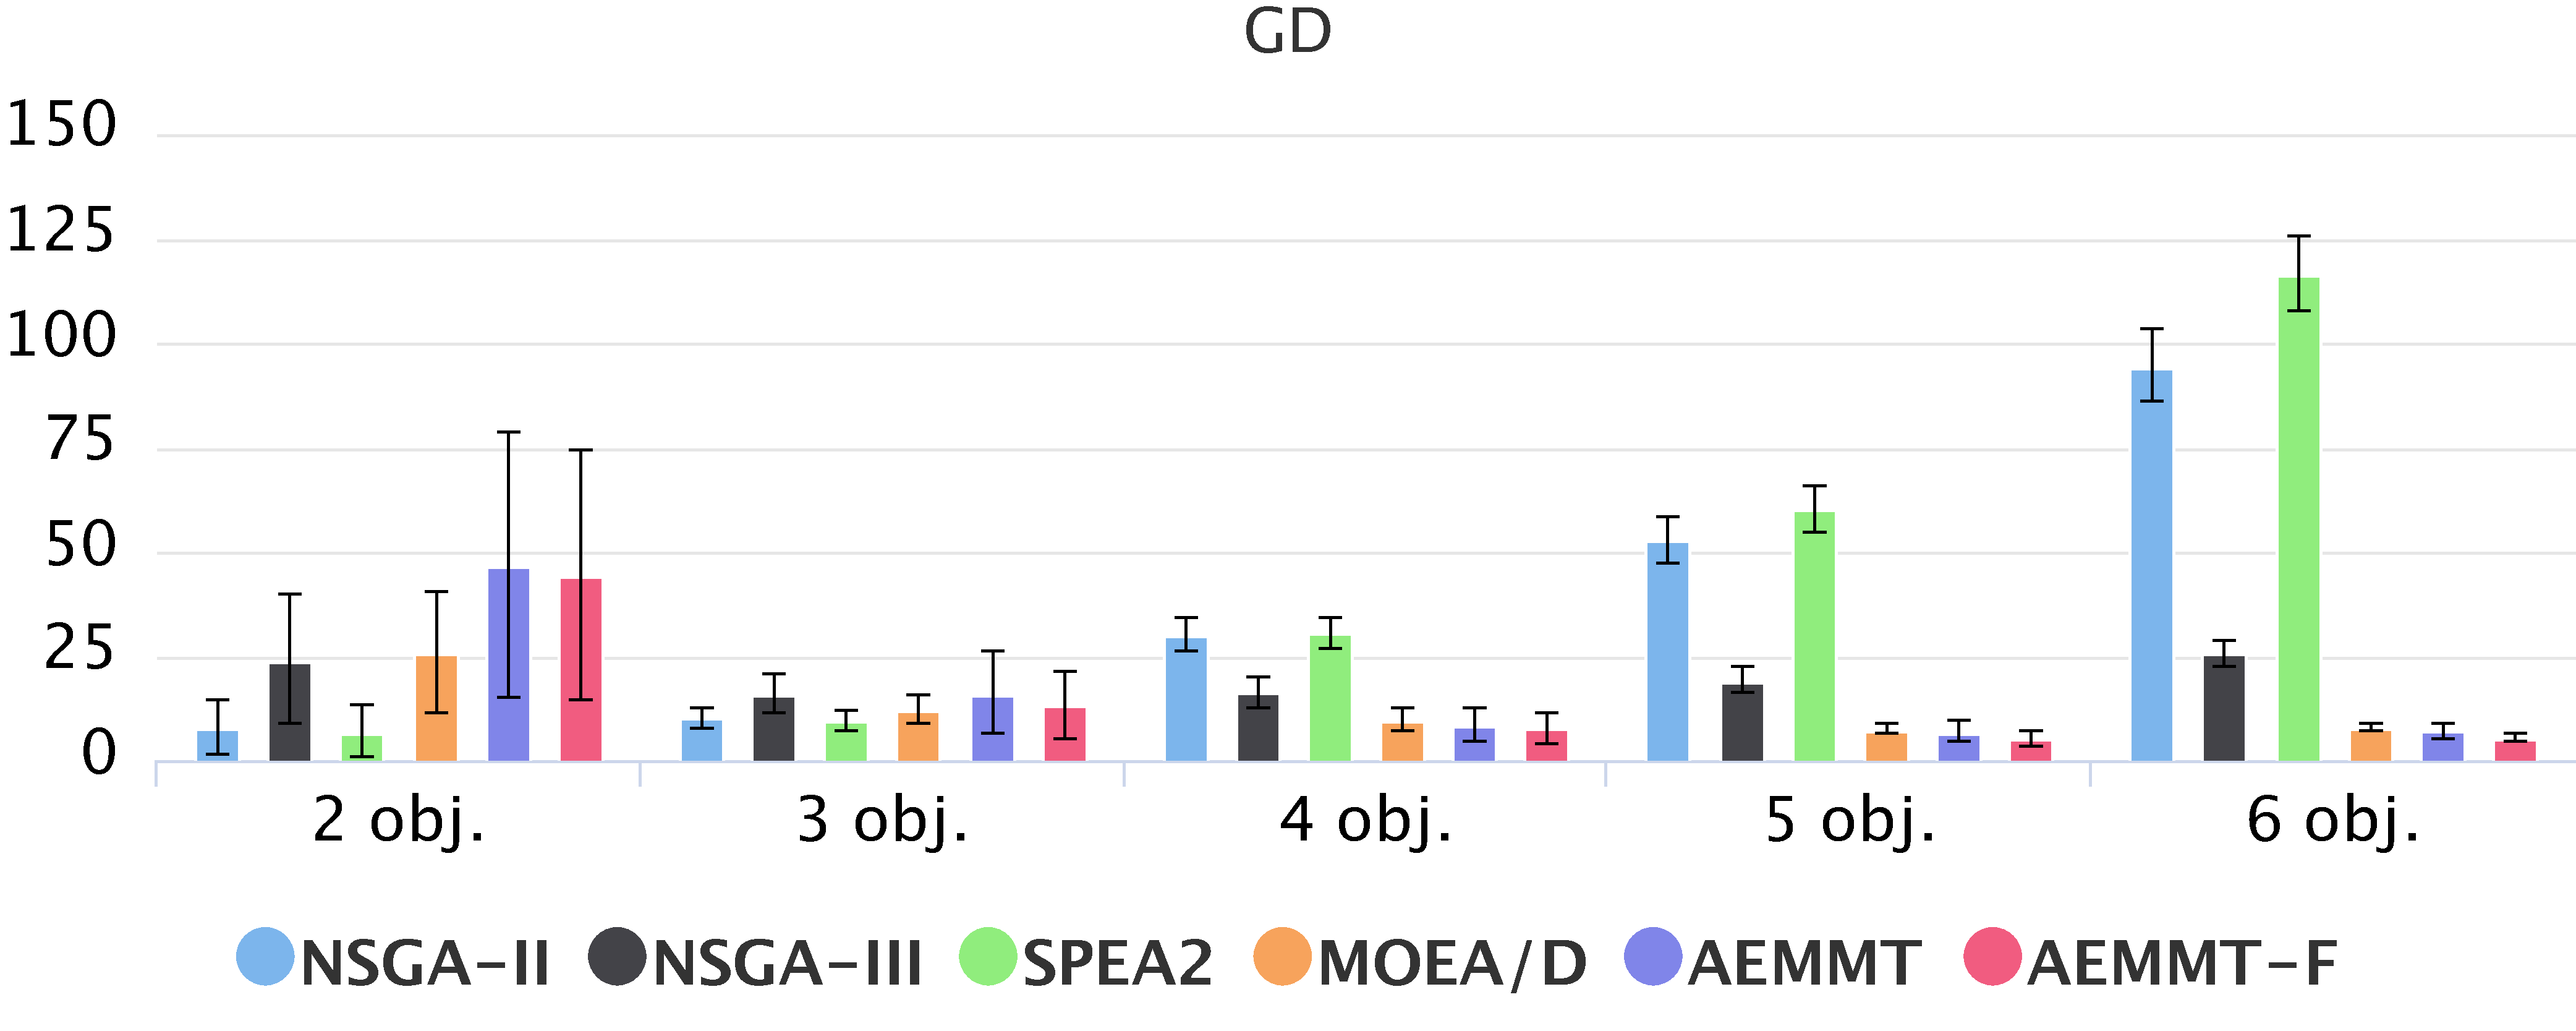
\includegraphics[width=1\textwidth]{cap_experimentos/figs/etapa1/gd-mkp-todos}
	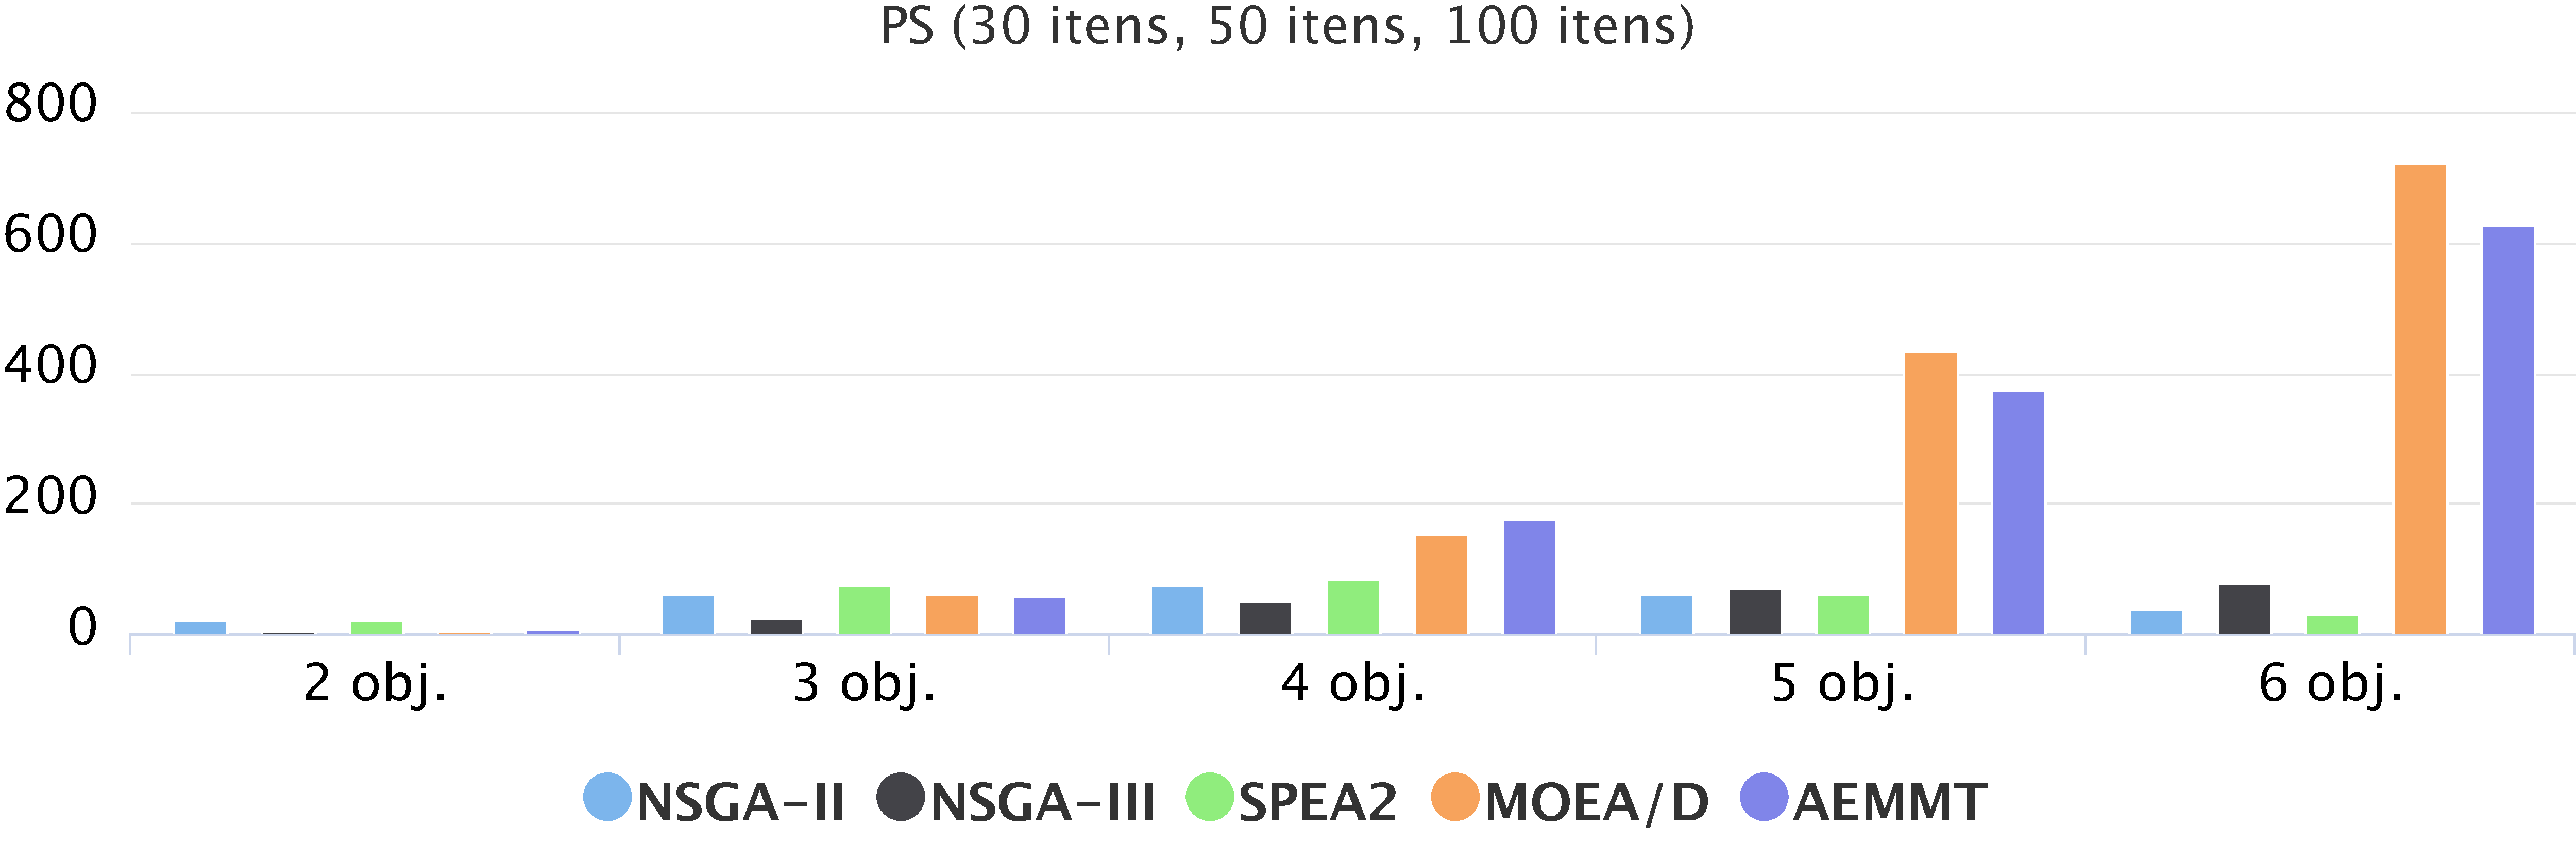
\includegraphics[width=1\textwidth]{cap_experimentos/figs/etapa1/ps-mkp-todos}
\end{figure*}

A figura \ref{fig_exp1_pmm_100} apresenta os resultados do PMM de 30, 50 e 100 itens de forma condensada para que se possa ver, de forma geral, o comportamento dos algoritmos nas diferentes formulações de objetivo. Os gráficos representam as médias entre os três cenários de dificuldade (30, 50 e 100 itens). Como esperado, considerando a literatura correlata, o NSGA-II e o SPEA2 são os melhores algoritmos para as formulações de 2 e 3 objetivos, apresentam melhor $ER$, $GD$ e $PS$. Por outro lado, a partir de 4 objetivos, o desempenho de ambos os algoritmos cai consideravelmente, enquanto o AEMMT assume a liderança. O NSGA-III, no problema de 4 objetivos, apresenta um erro quase tão baixo quanto o AEMMT, mas seu $GD$ e $PS$ são piores. o MOEA/D, para 5 e 6 objetivos, apresenta o segundo melhor resultado em qualquer uma das métricas. Em resumo, o NSGA-III não parece uma boa opção em nenhum dos casos, pois sempre há outro algoritmo que o supera. O NSGA-II e o SPEA2 são igualmente bons e os melhores em problemas com poucos objetivos. O AEMMT e o MOEA/D são ótimas opções para problemas a partir de 4 objetivos, sendo que o MOEA/D confere um melhor $PS$ enquanto o AEMMT providencia menor taxa de erro.

\begin{figure*}[!htbp]
	\caption{Etapa 1: resultados para o PRM na rede $R_1$}
	\label{fig_exp1_prm_r1}
	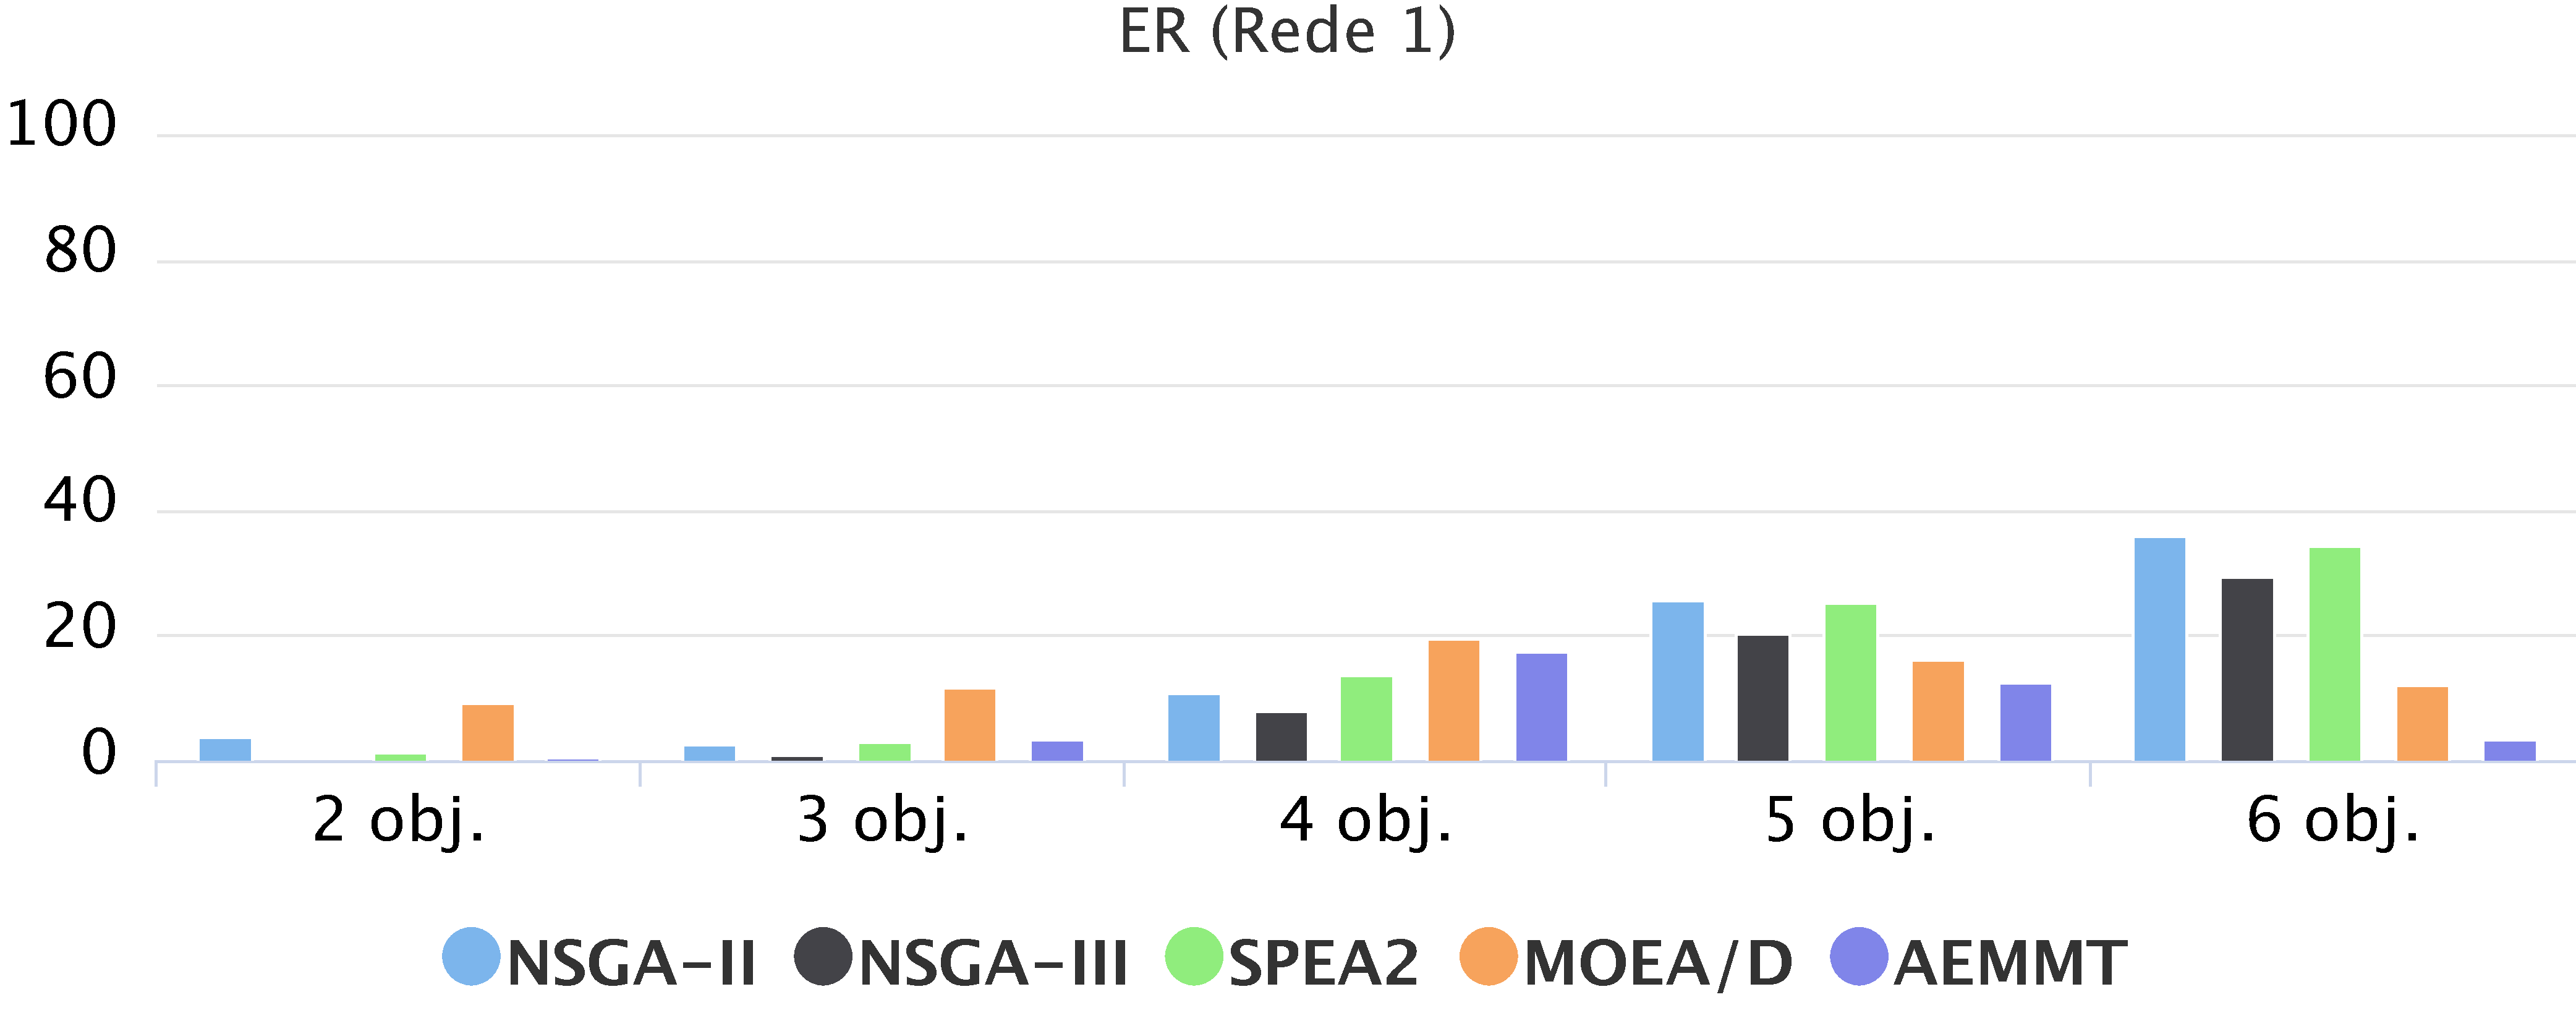
\includegraphics[width=1\textwidth]{cap_experimentos/figs/etapa1/er-mrp-r1}
	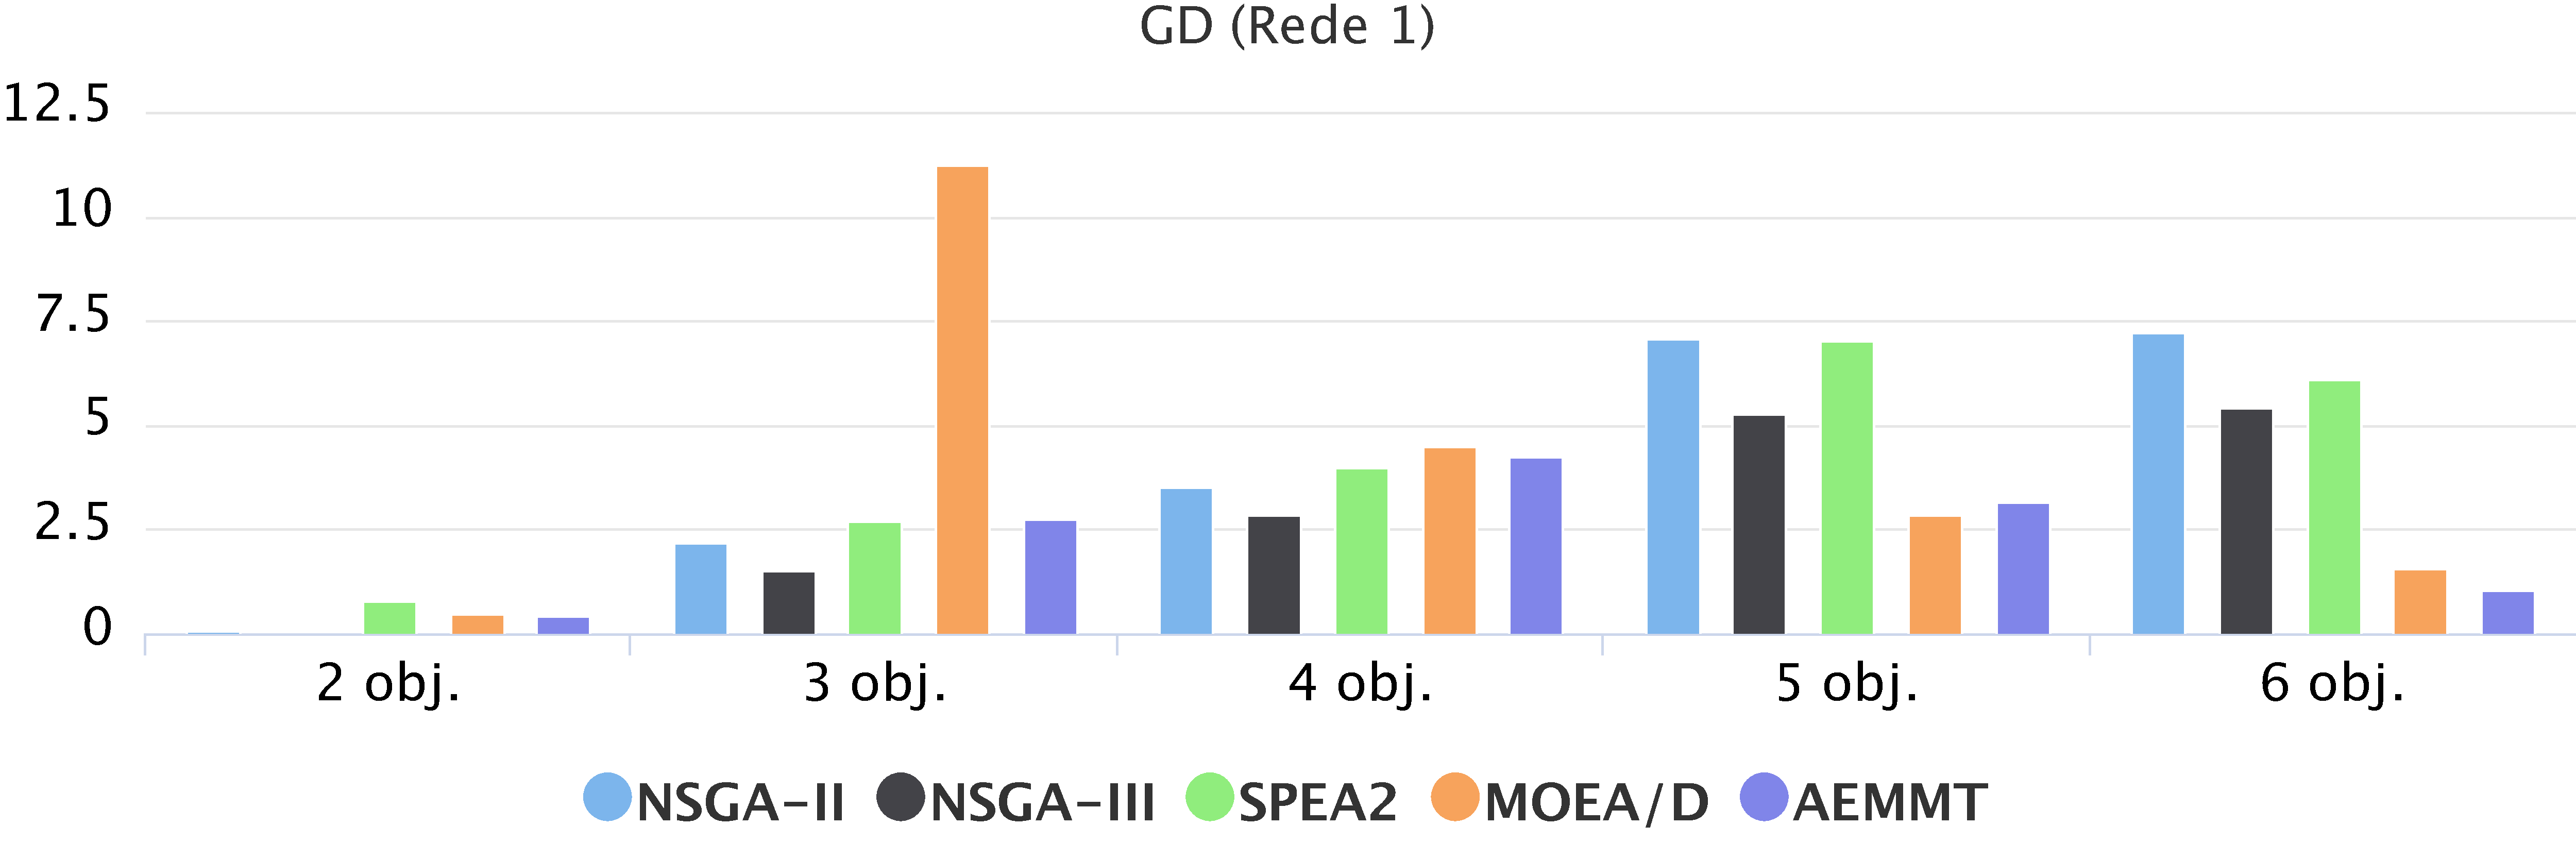
\includegraphics[width=1\textwidth]{cap_experimentos/figs/etapa1/gd-mrp-r1}
	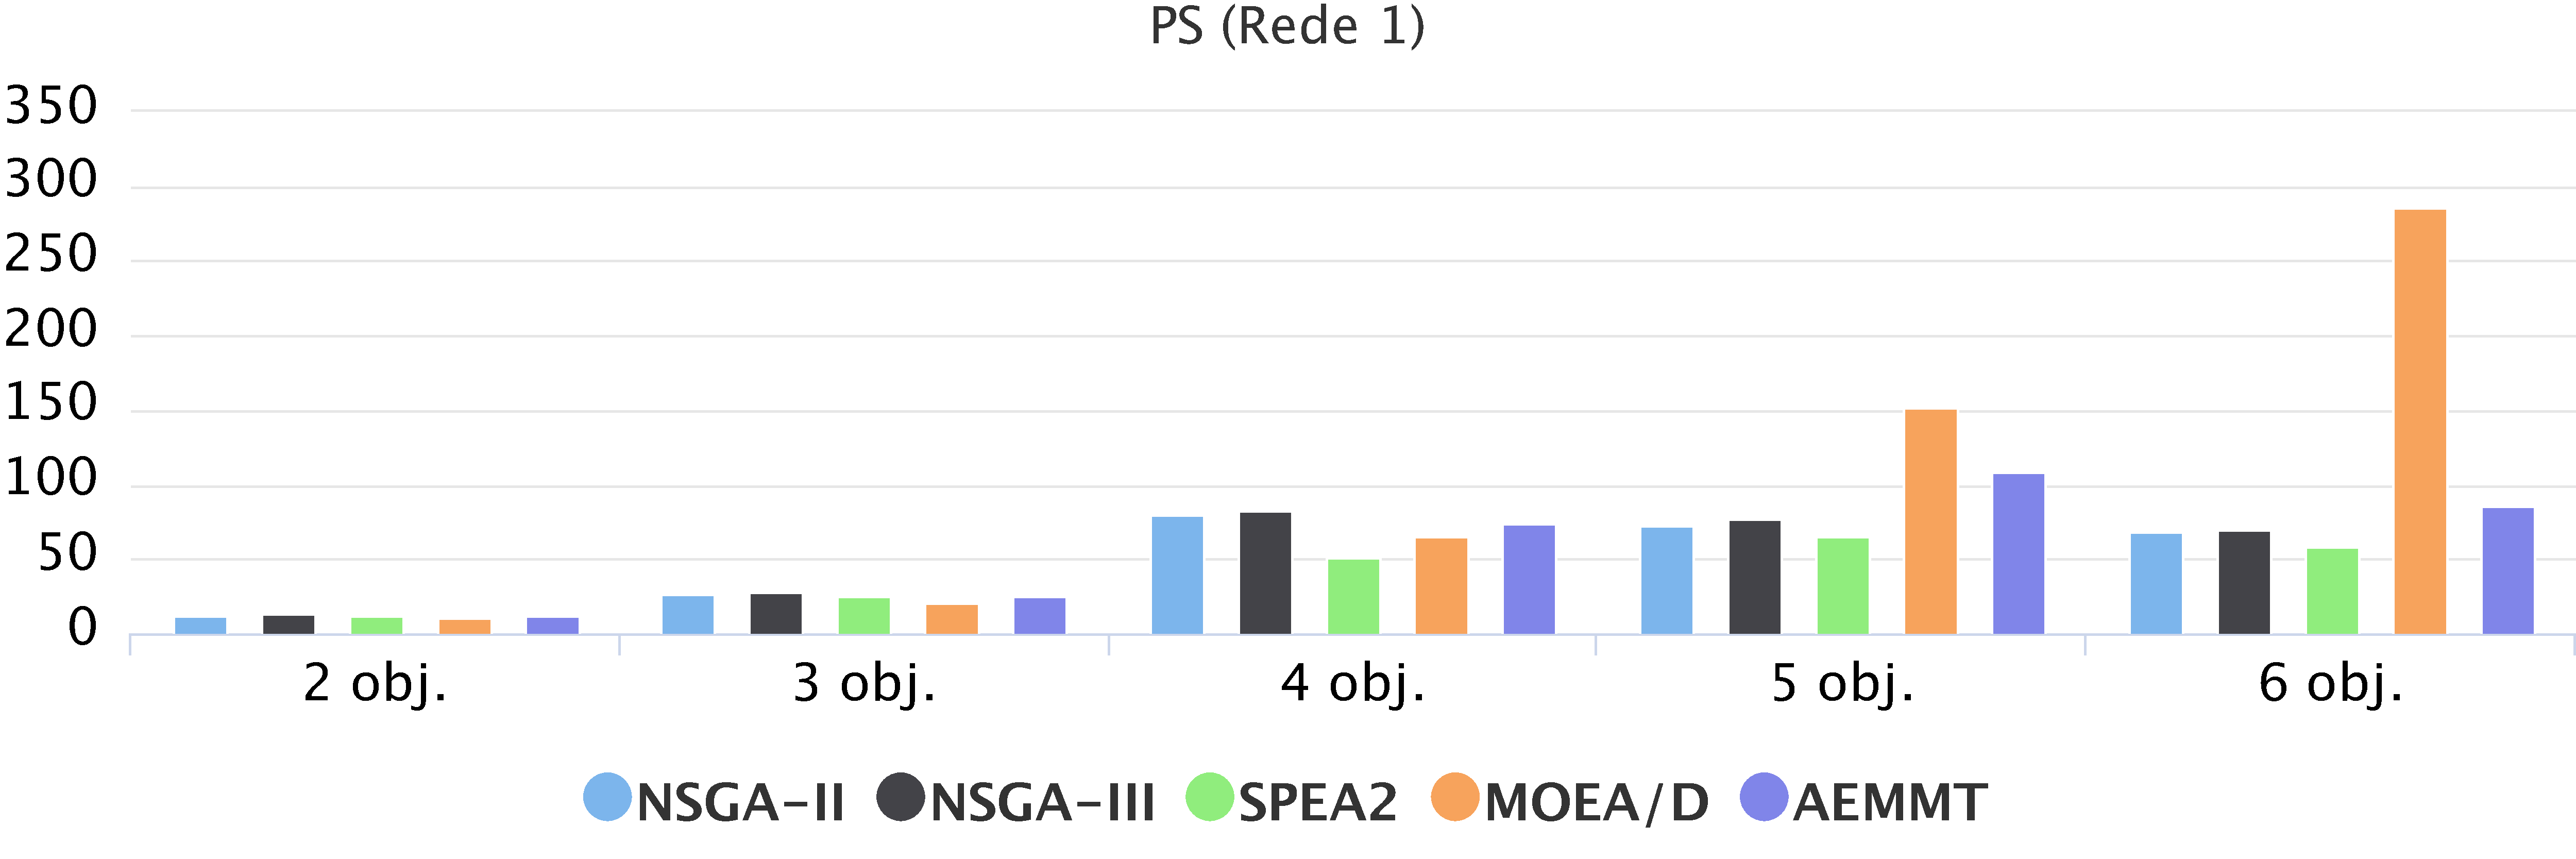
\includegraphics[width=1\textwidth]{cap_experimentos/figs/etapa1/ps-mrp-r1}
\end{figure*}

O PRM sobre a rede 1 (figura \ref{fig_exp1_prm_r1}), a mais simples dentre elas, mostrou bons resultados para todos os algoritmos. Diferente do esperado, o NSGA-III mostrou o melhor resultado ($ER$, $GD$ e $PS$) para os problemas com 2, 3 e 4 objetivos. A partir de 5 objetivos, o AEMMT e o MOEA/D são os dois melhores métodos, o primeiro apresenta uma menor taxa de erro, enquanto o segundo obtém um Pareto de maior cardinalidade. Para poucos objetivos, o NSGA-III é claramente o melhor método, para 5 ou mais critérios de otimização, ambos AEMMT e MOEA/D são boas opções.

\begin{figure*}[!htbp]
	\caption{Etapa 1: resultados para o PRM na rede $R_2$}
	\label{fig_exp1_prm_r2}
	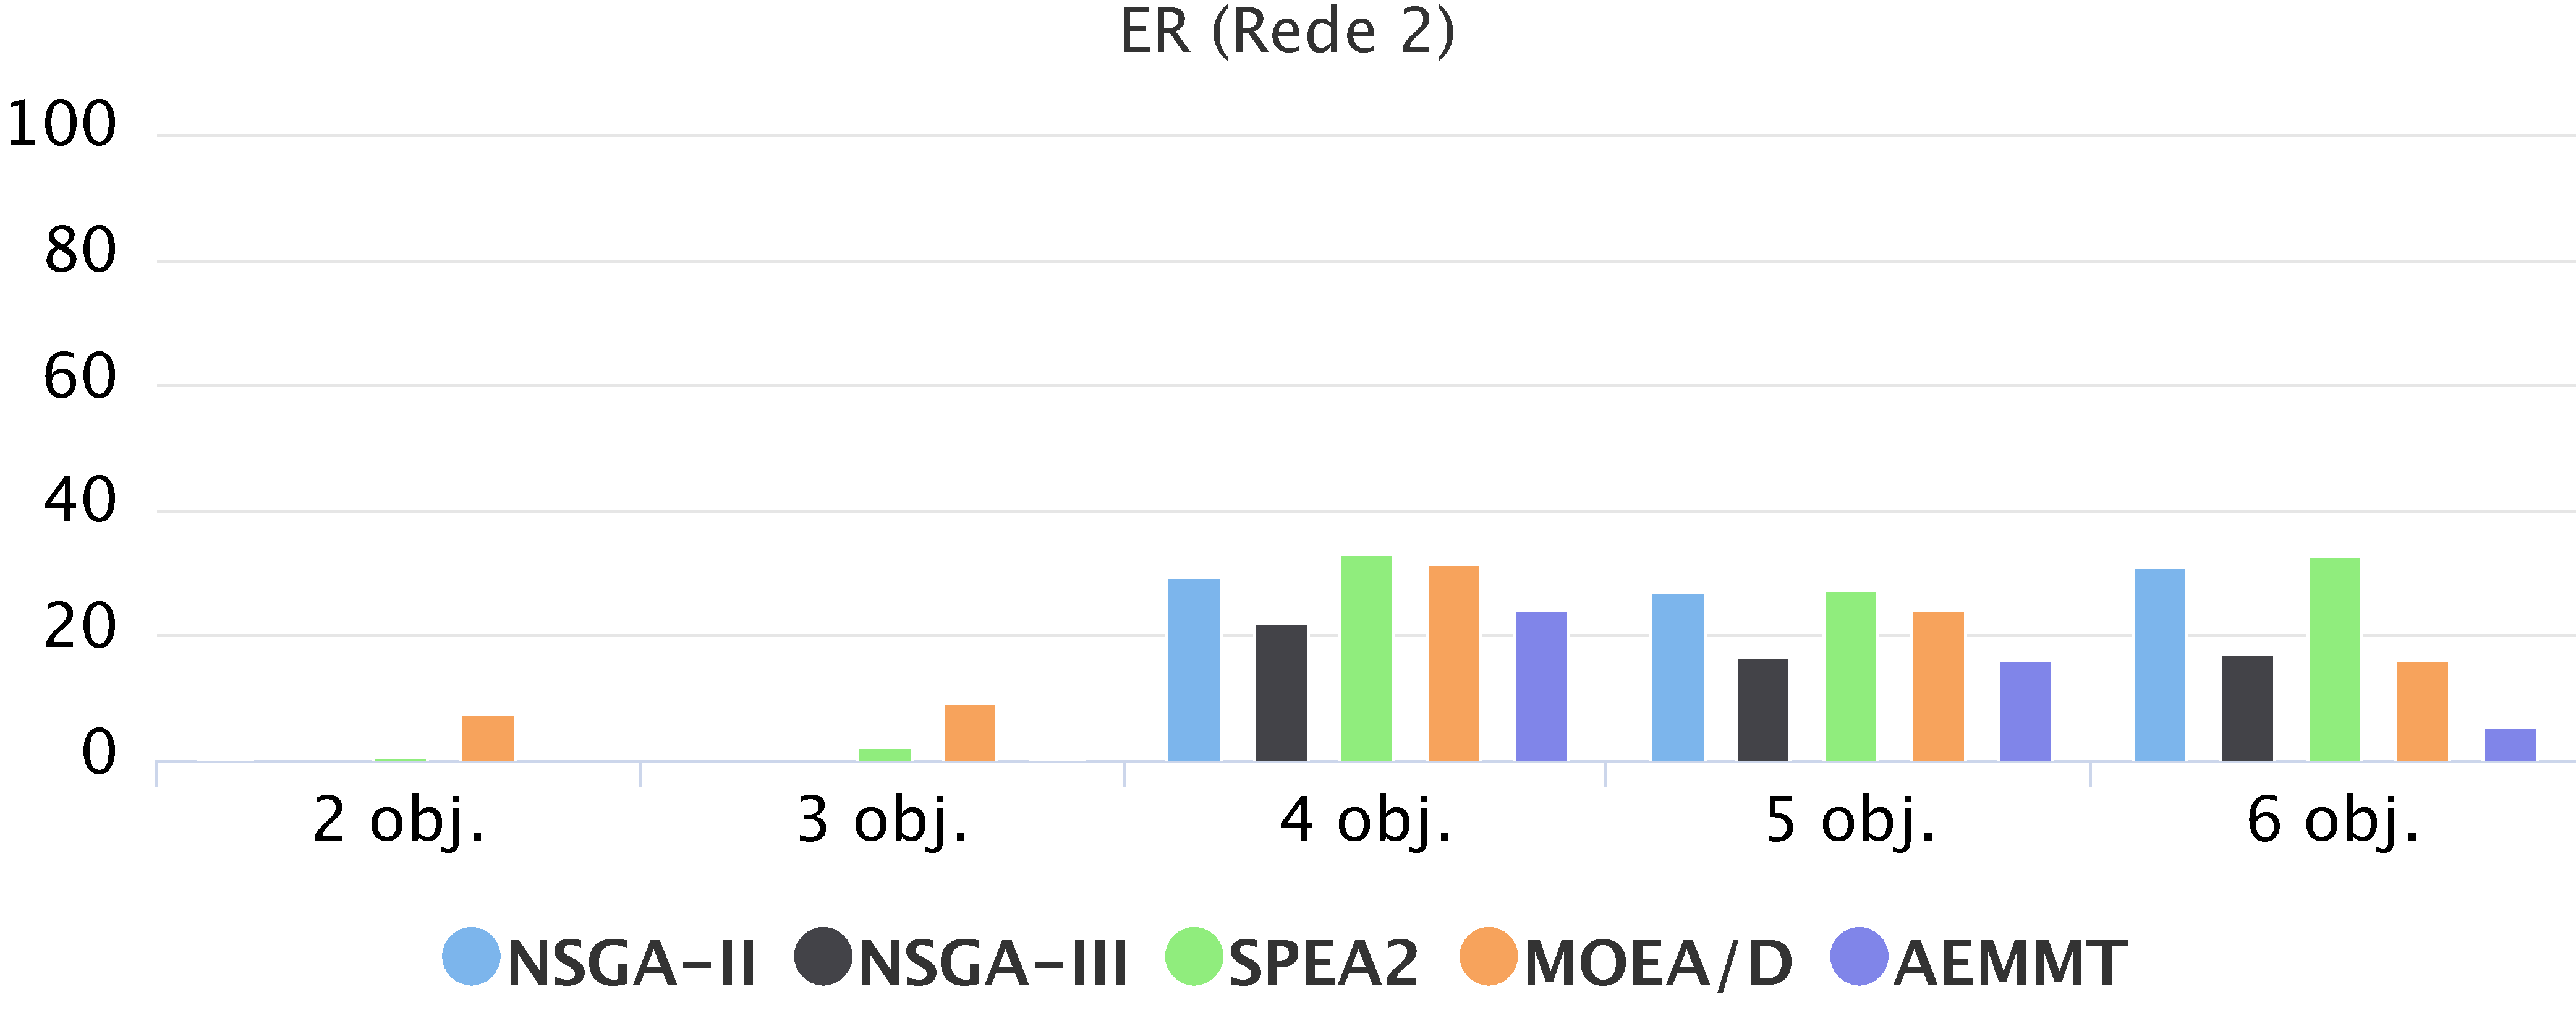
\includegraphics[width=1\textwidth]{cap_experimentos/figs/etapa1/er-mrp-r2}
	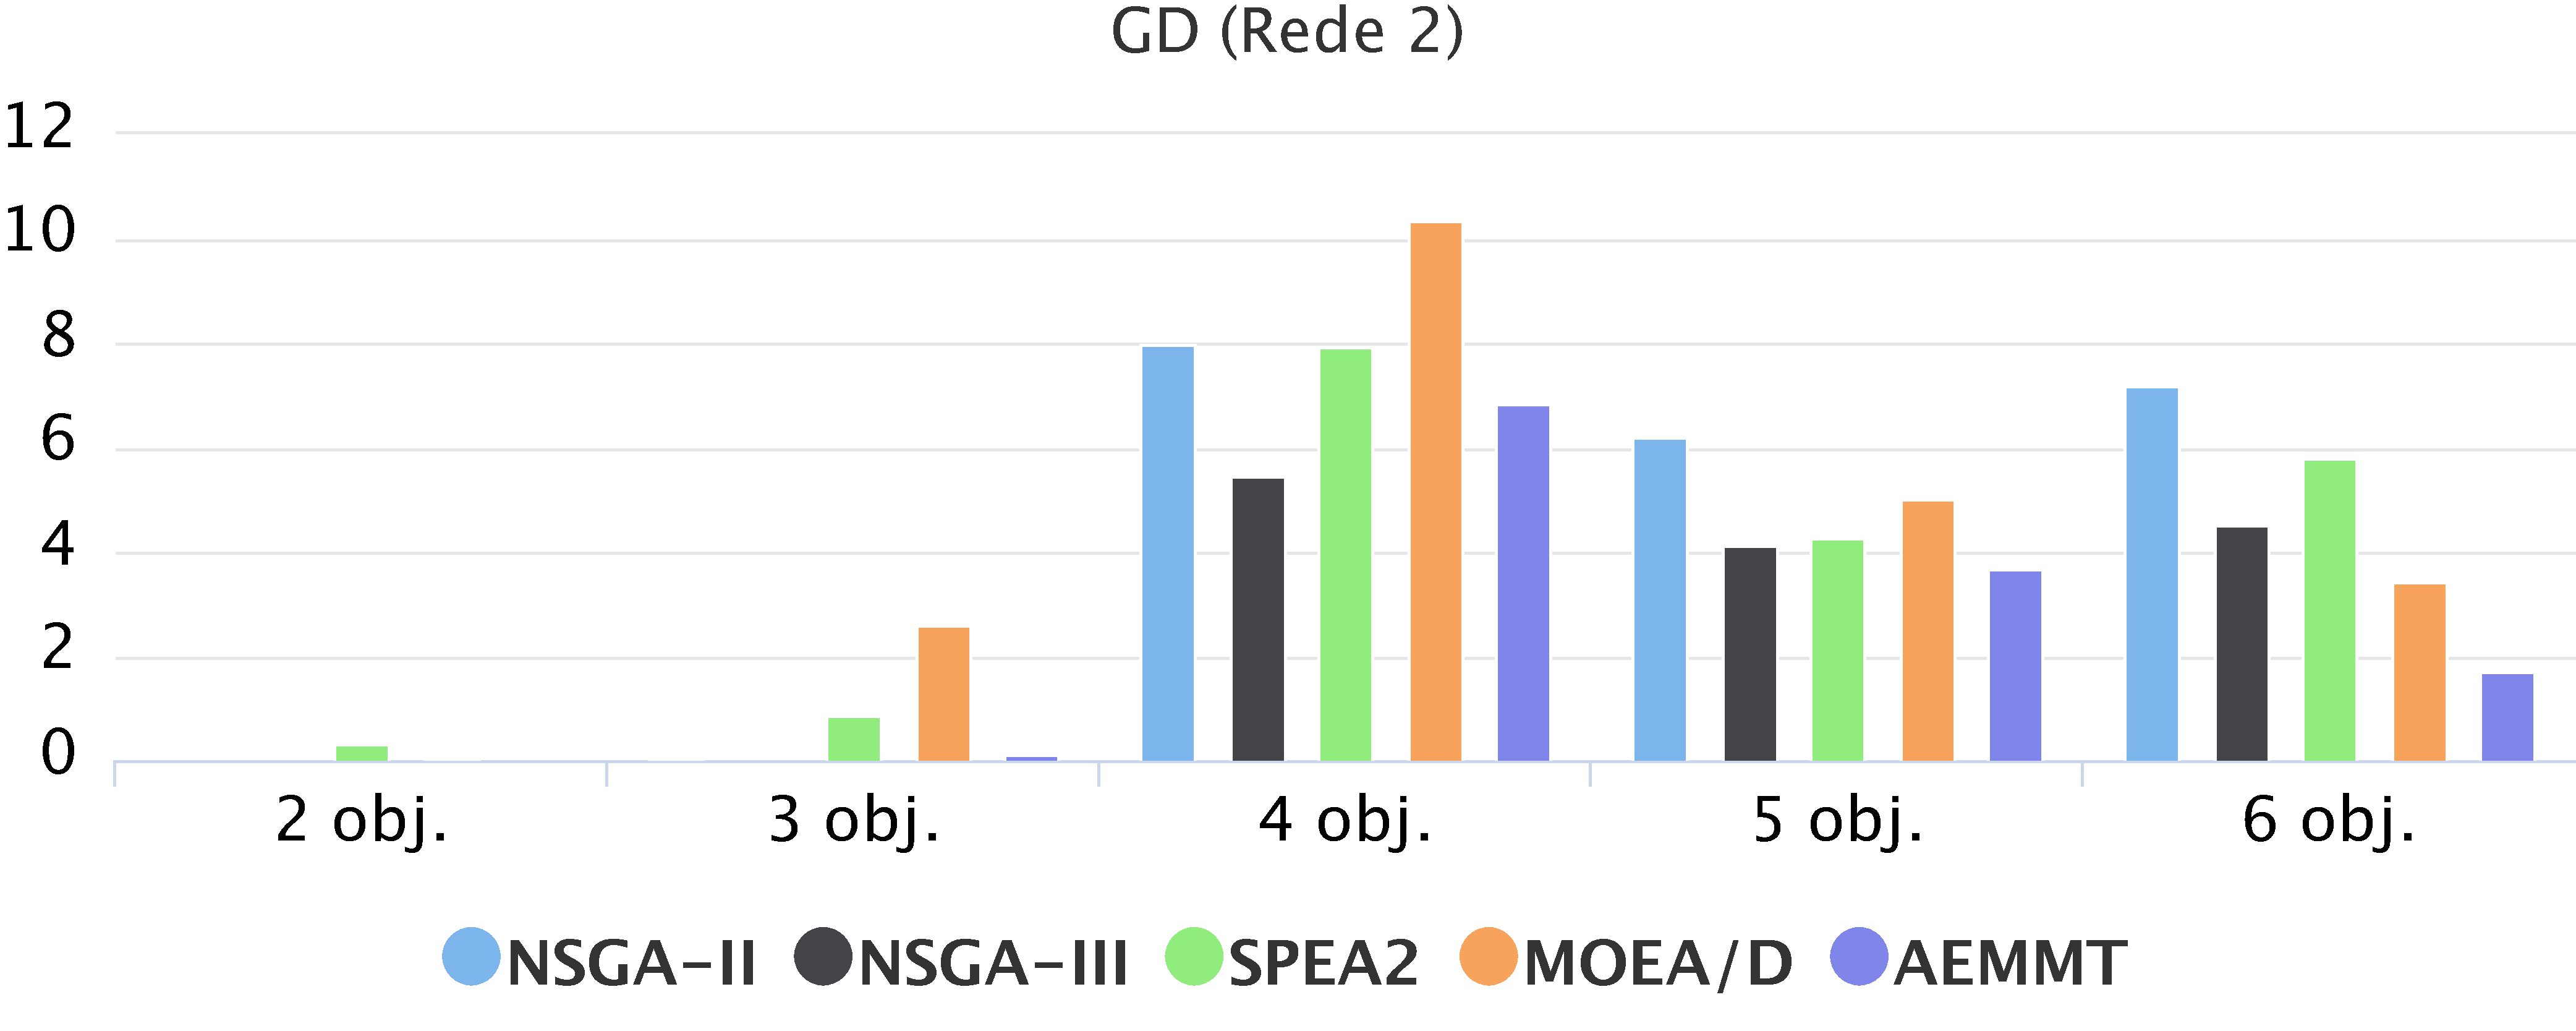
\includegraphics[width=1\textwidth]{cap_experimentos/figs/etapa1/gd-mrp-r2}
	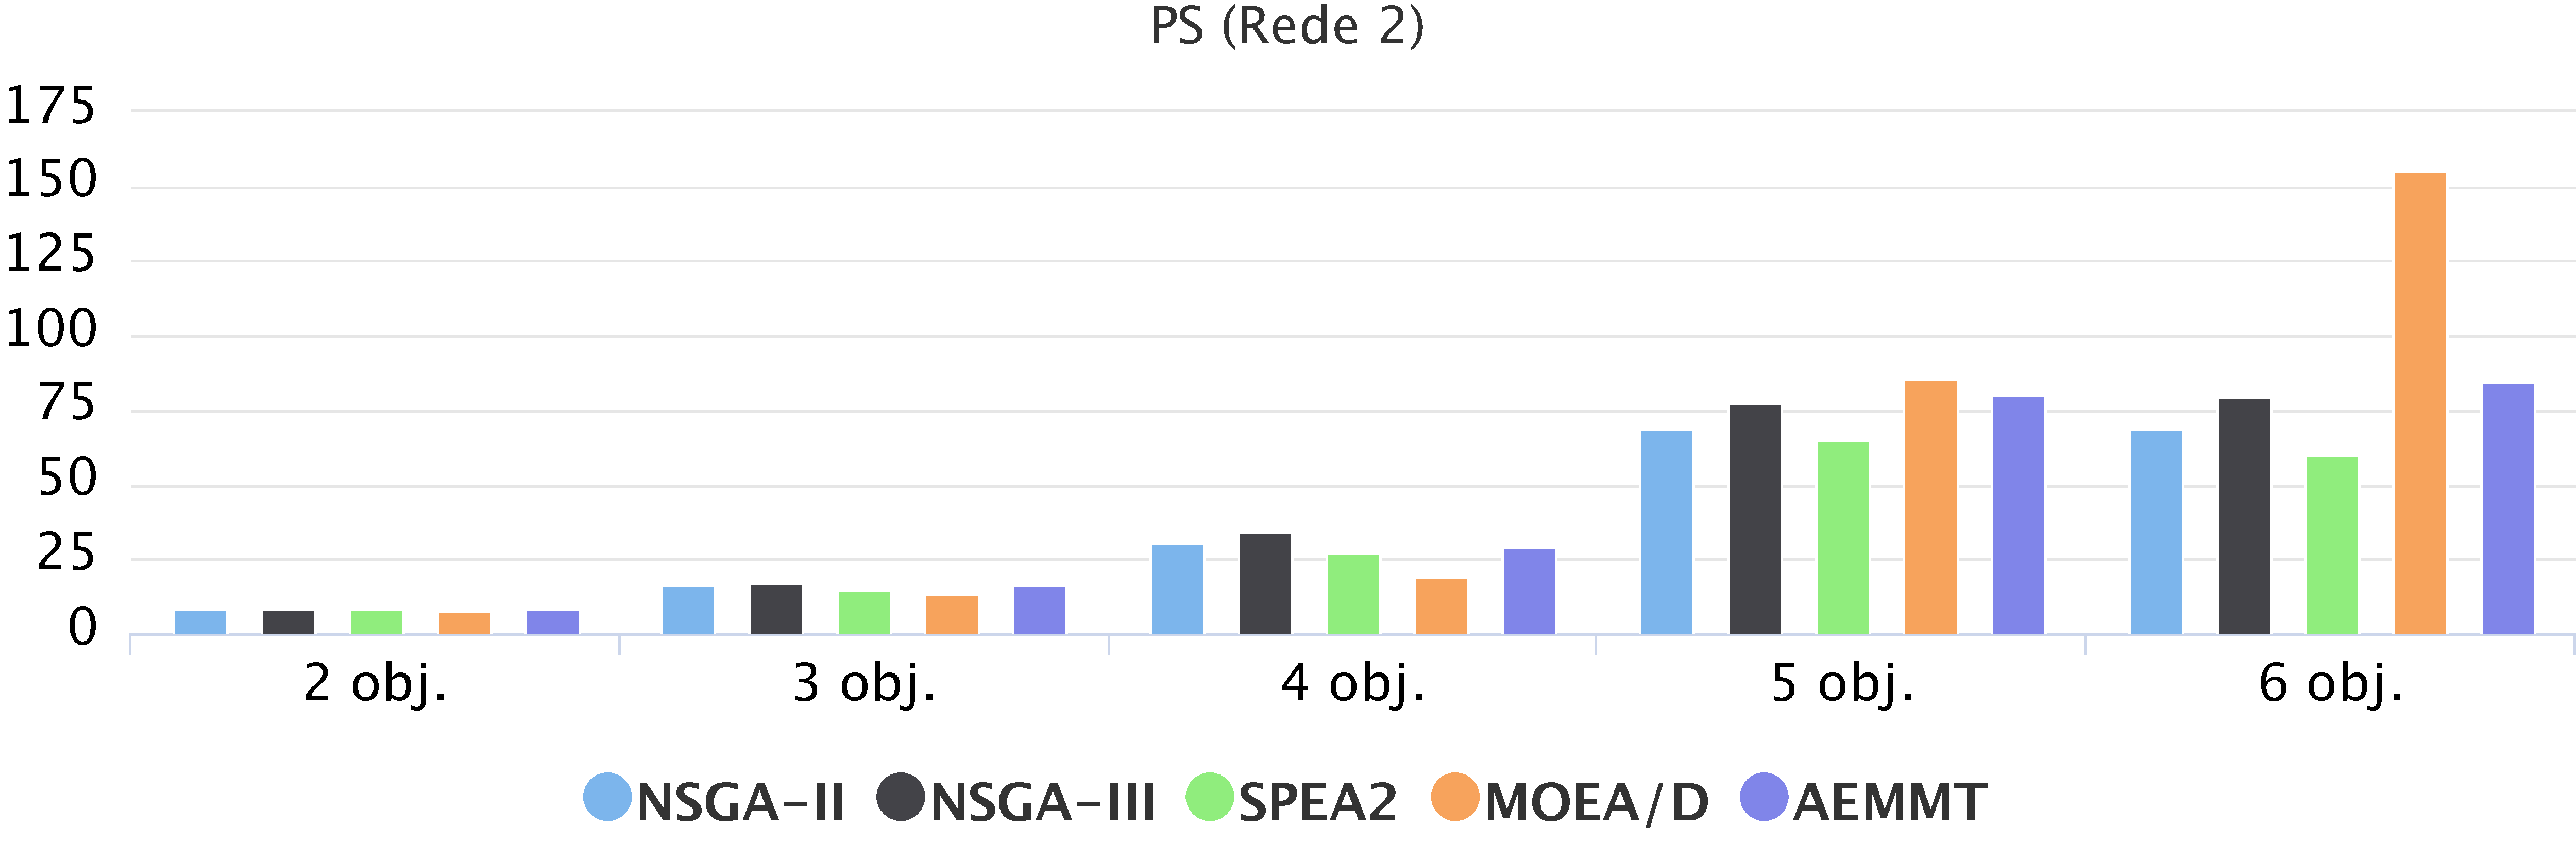
\includegraphics[width=1\textwidth]{cap_experimentos/figs/etapa1/ps-mrp-r2}
\end{figure*}

Na rede 2 (figura \ref{fig_exp1_prm_r2}), o NSGA-III é o melhor algoritmo nos problemas com 2, 3, 4 e 5 objetivos, perdendo, por pouco, apenas em $PS$ para o AEMMT e o MOEA/D no problema de 5 objetivos. Com 6 objetivos, o AEMMT é o melhor algoritmo quando se considera o erro e o $GD$, mas se um maior $PS$ é mais desejável, então o MOEA/D é o método mais adequado.

\begin{figure*}[!htbp]
	\caption{Etapa 1: resultados para o PRM na rede $R_3$}
	\label{fig_exp1_prm_r3}
	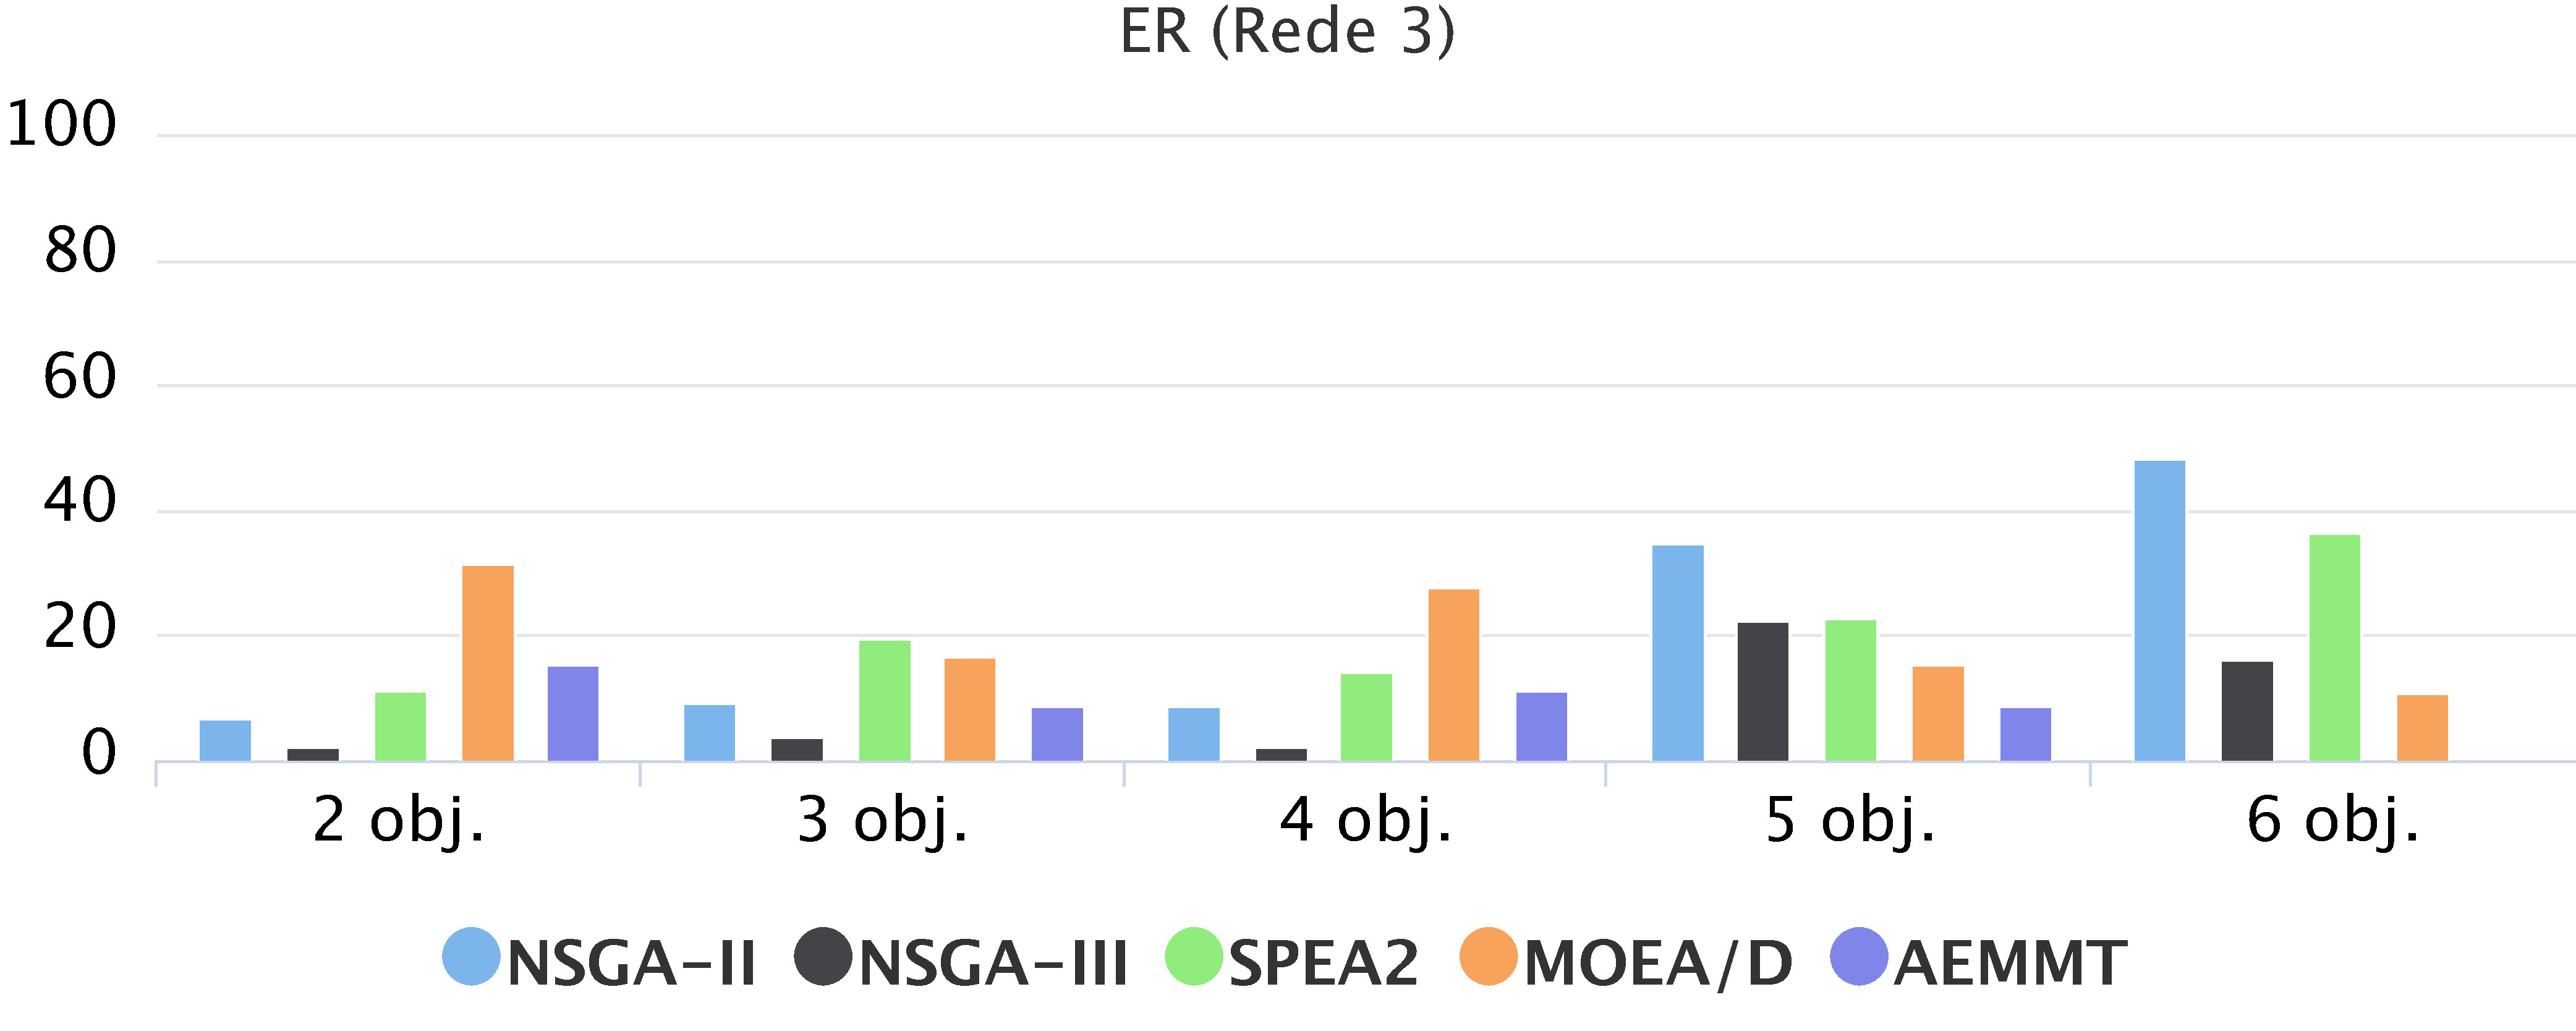
\includegraphics[width=1\textwidth]{cap_experimentos/figs/etapa1/er-mrp-r3}
	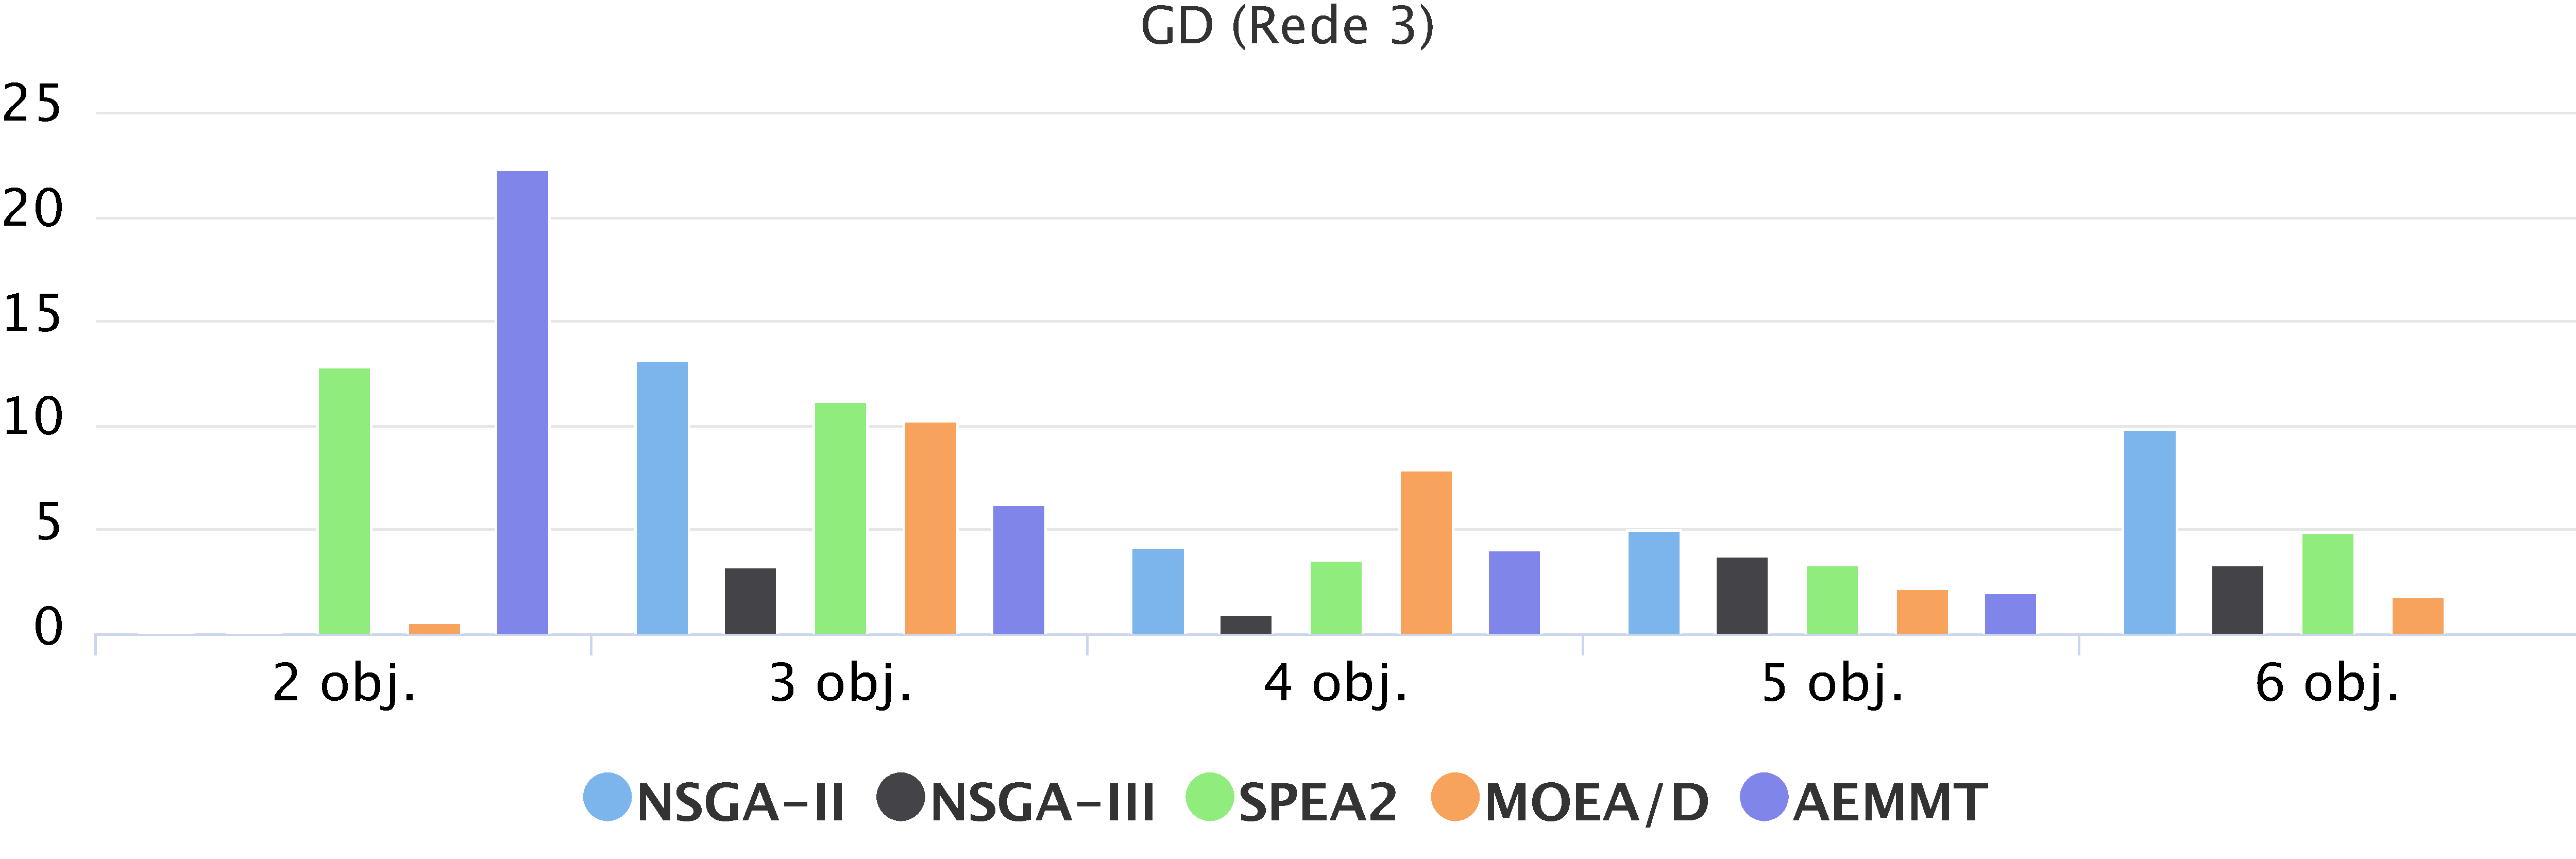
\includegraphics[width=1\textwidth]{cap_experimentos/figs/etapa1/gd-mrp-r3}
	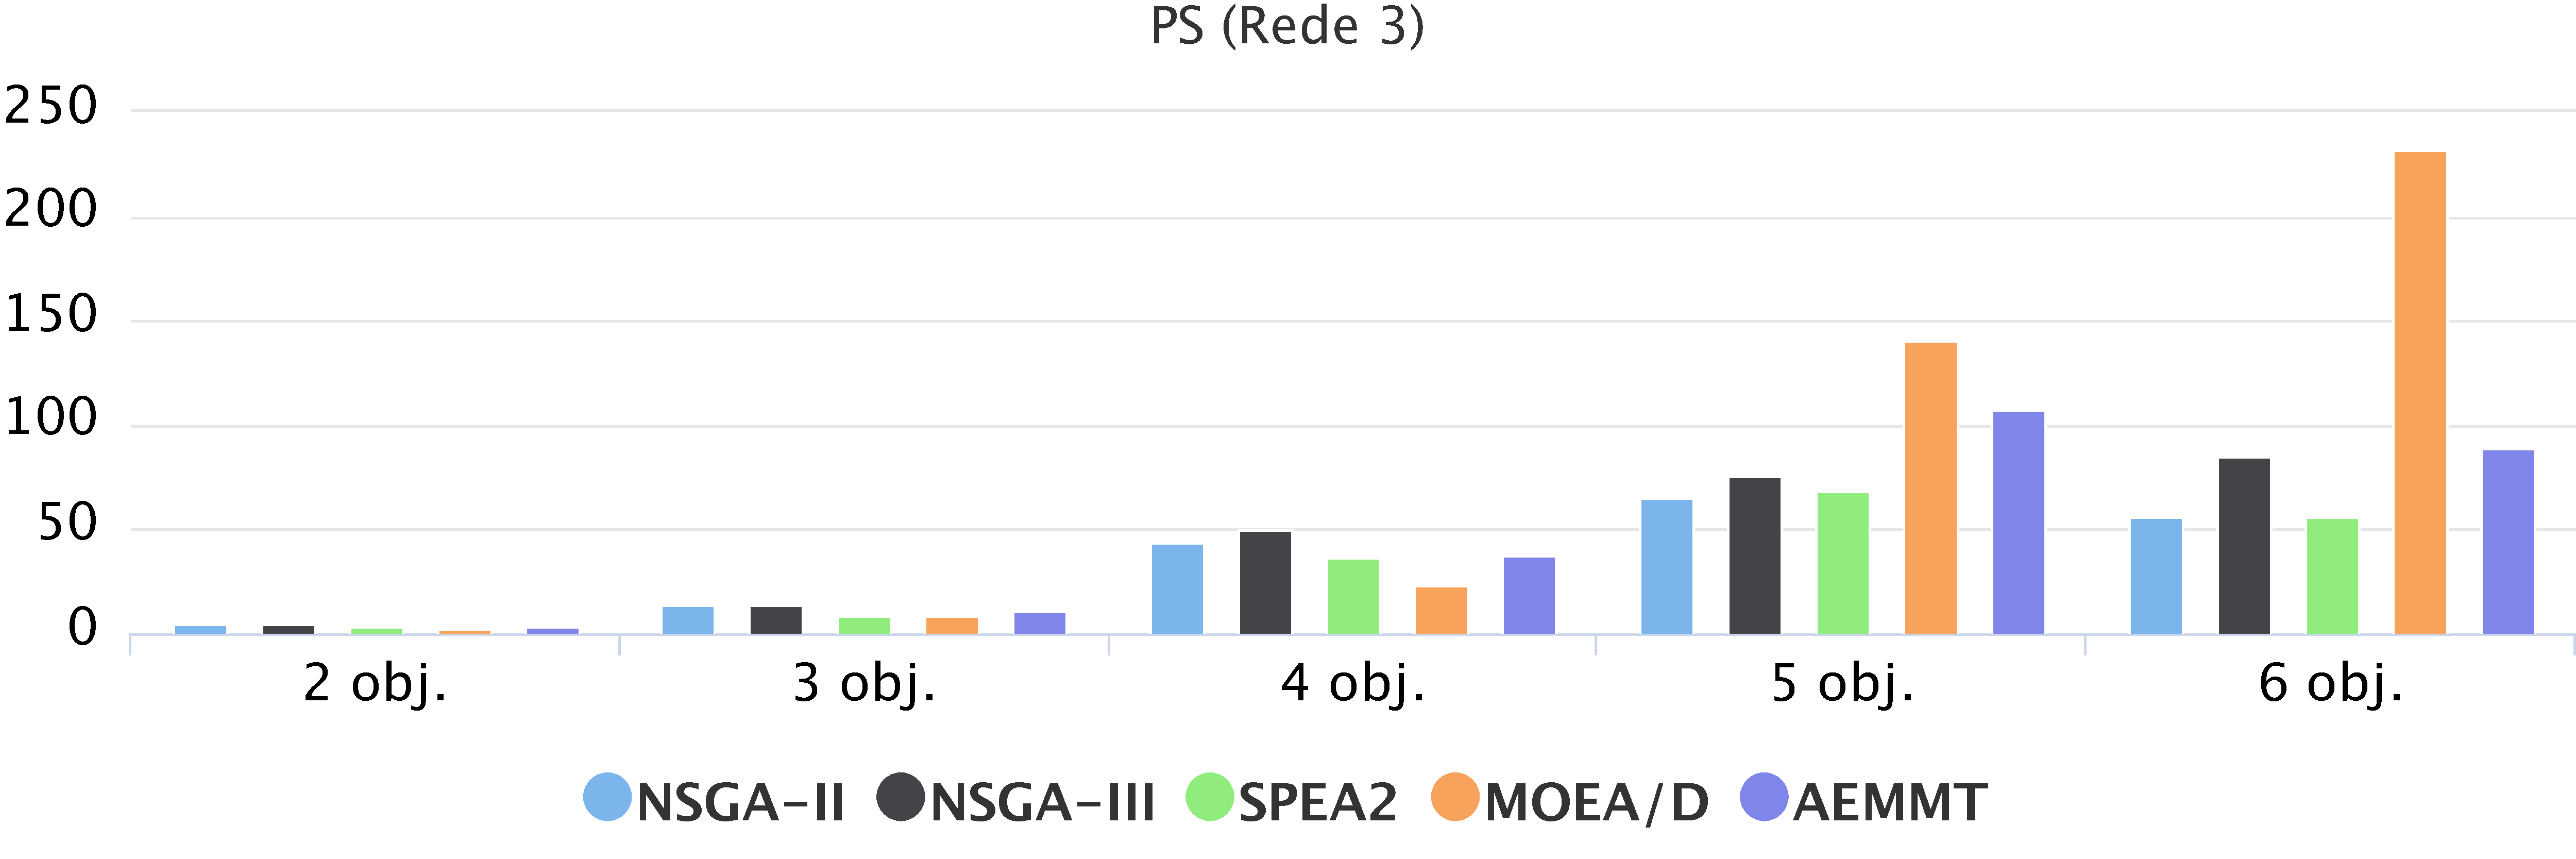
\includegraphics[width=1\textwidth]{cap_experimentos/figs/etapa1/ps-mrp-r3}
\end{figure*}

A rede 3 (figura \ref{fig_exp1_prm_r3}) é a mais complexa analisada nesta etapa dos experimentos. Nela, a tendência já observada do NSGA-III de ser o melhor método para poucos objetivos continua. Até 4 objetivos, em todas as métricas, o NSGA-III apresenta os melhores resultados. Para 5 e 6 critérios de otimização, o AEMMT apresenta menor $ER$ e $GD$, enquanto o MOEA/D consegue maior $PS$.

\begin{figure*}[!htbp]
	\caption{Etapa 1: resultados agrupados para o PRM nas redes $R_1$, $R_2$ e $R_3$}
	\label{fig_exp1_prm_todos}
	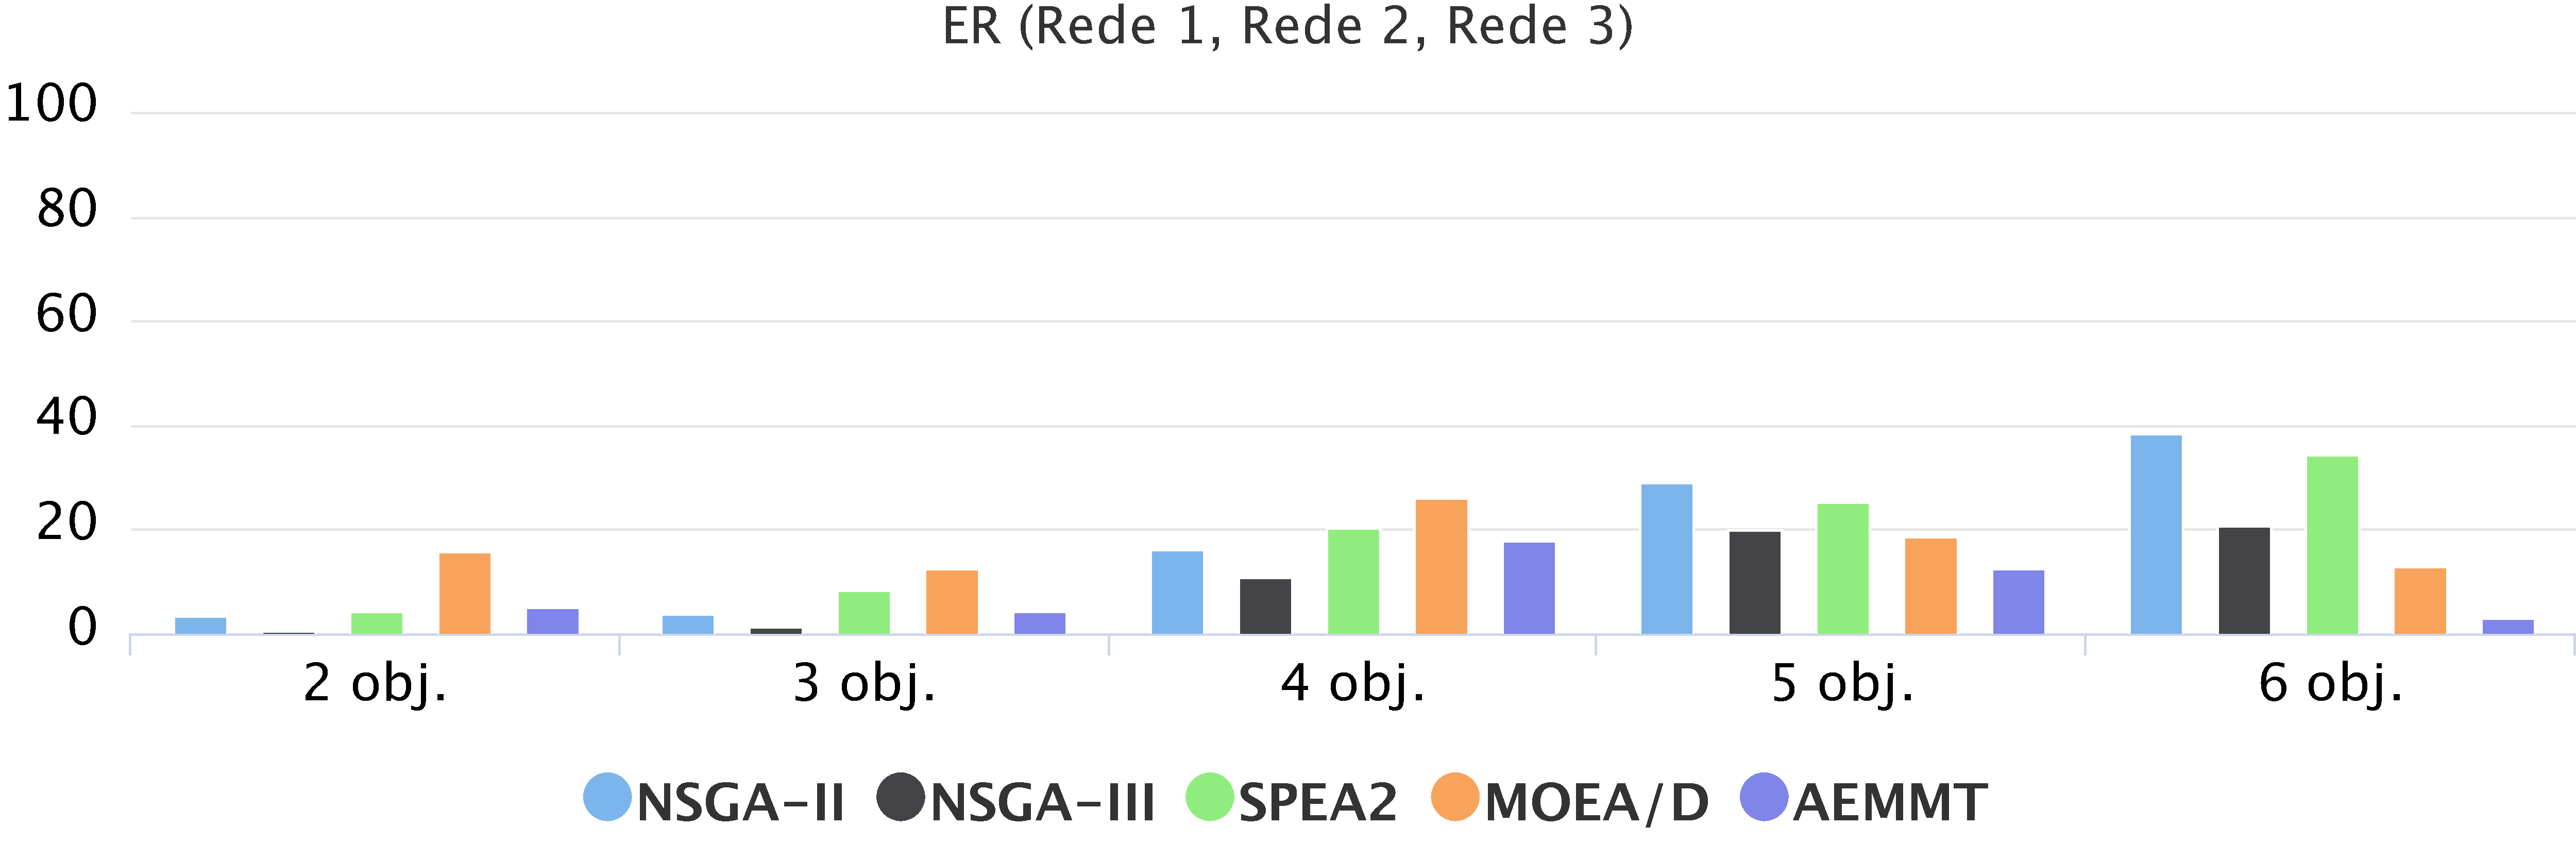
\includegraphics[width=1\textwidth]{cap_experimentos/figs/etapa1/er-mrp-todos}
	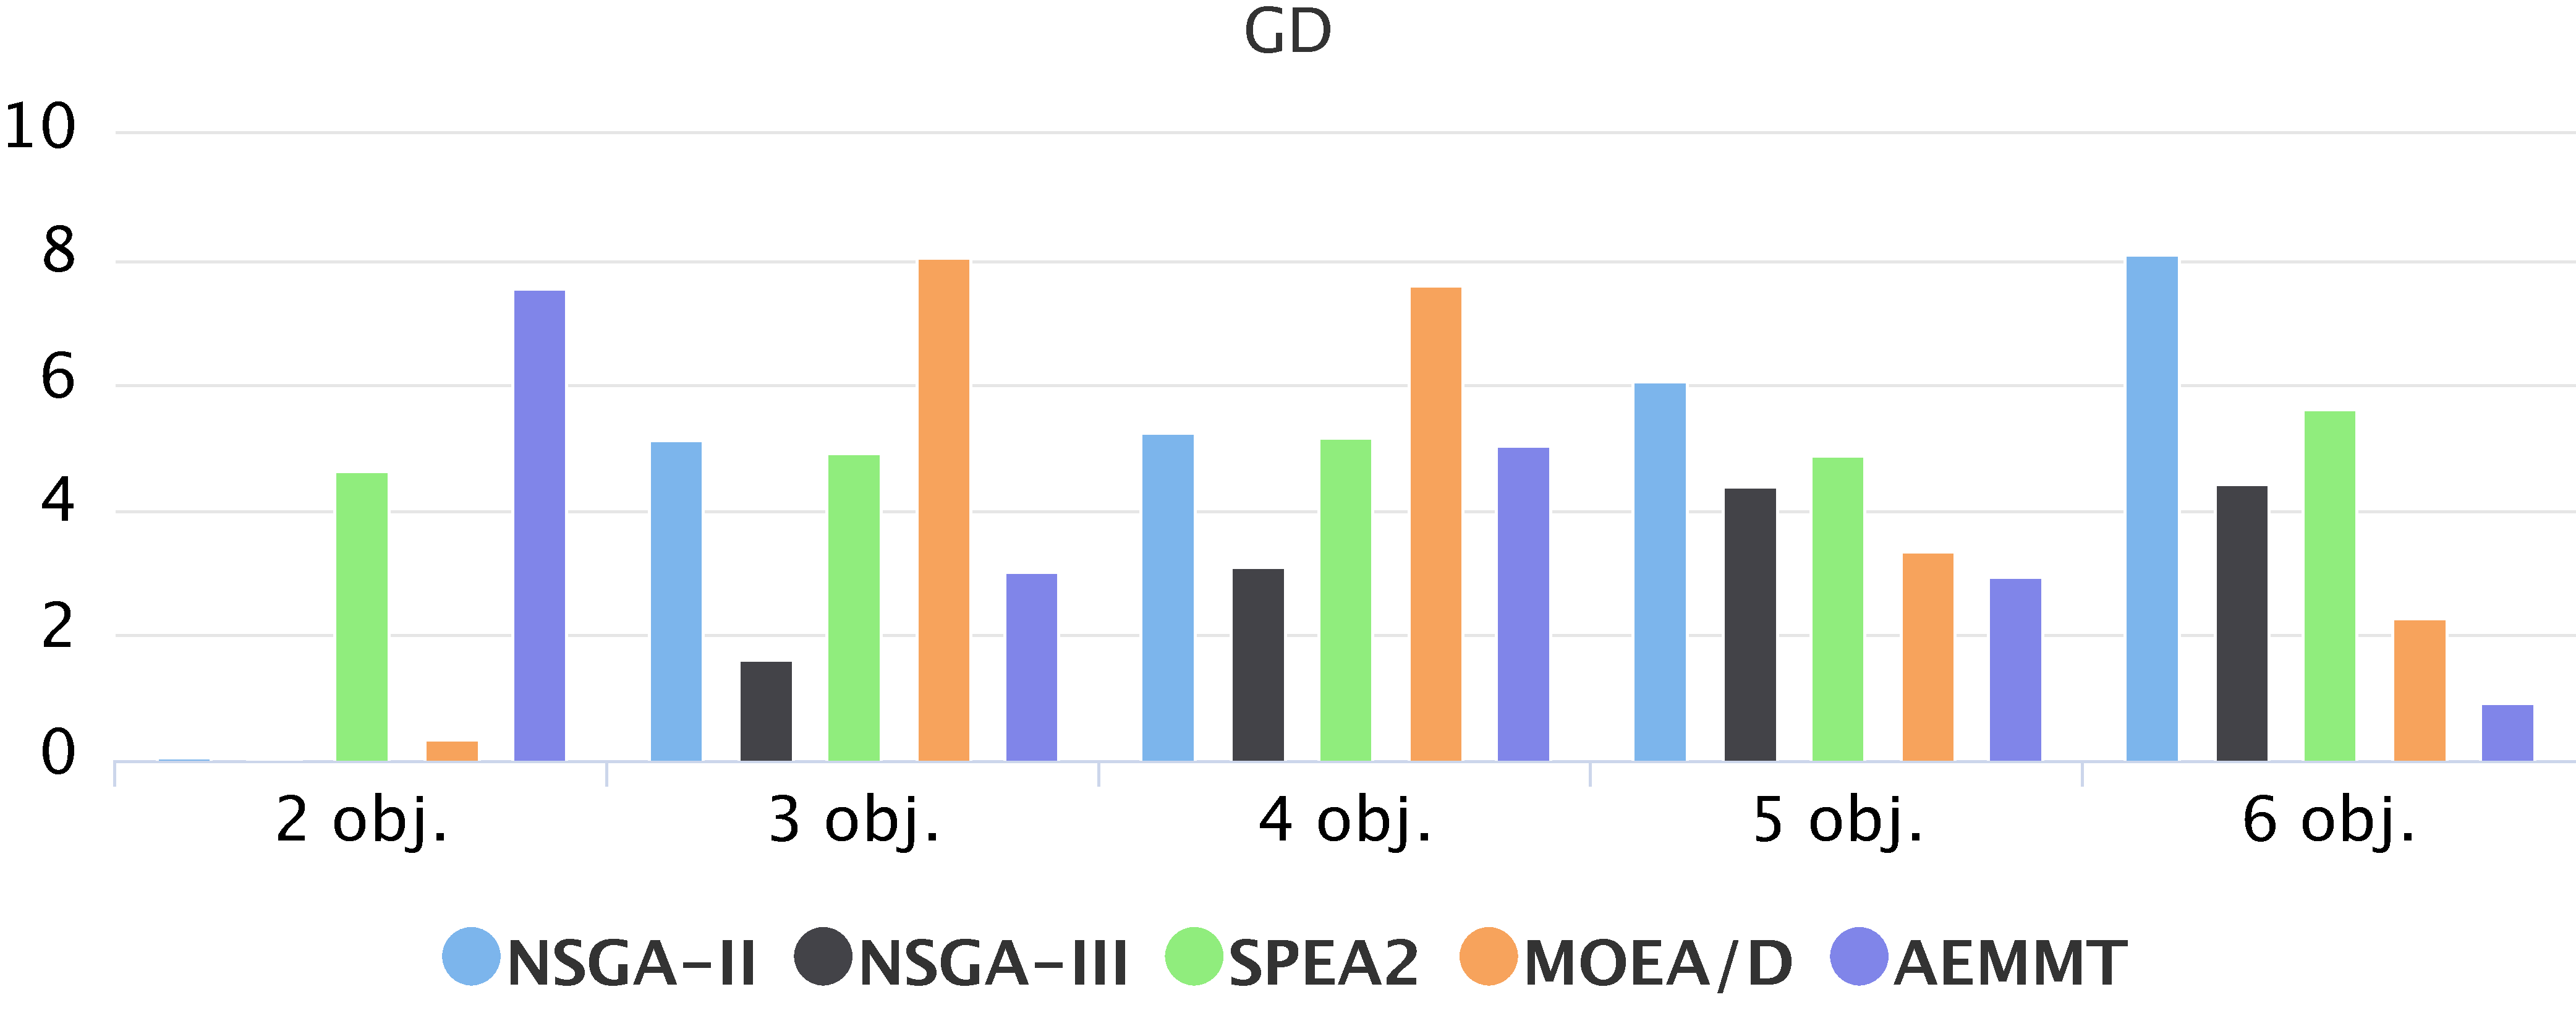
\includegraphics[width=1\textwidth]{cap_experimentos/figs/etapa1/gd-mrp-todos}
	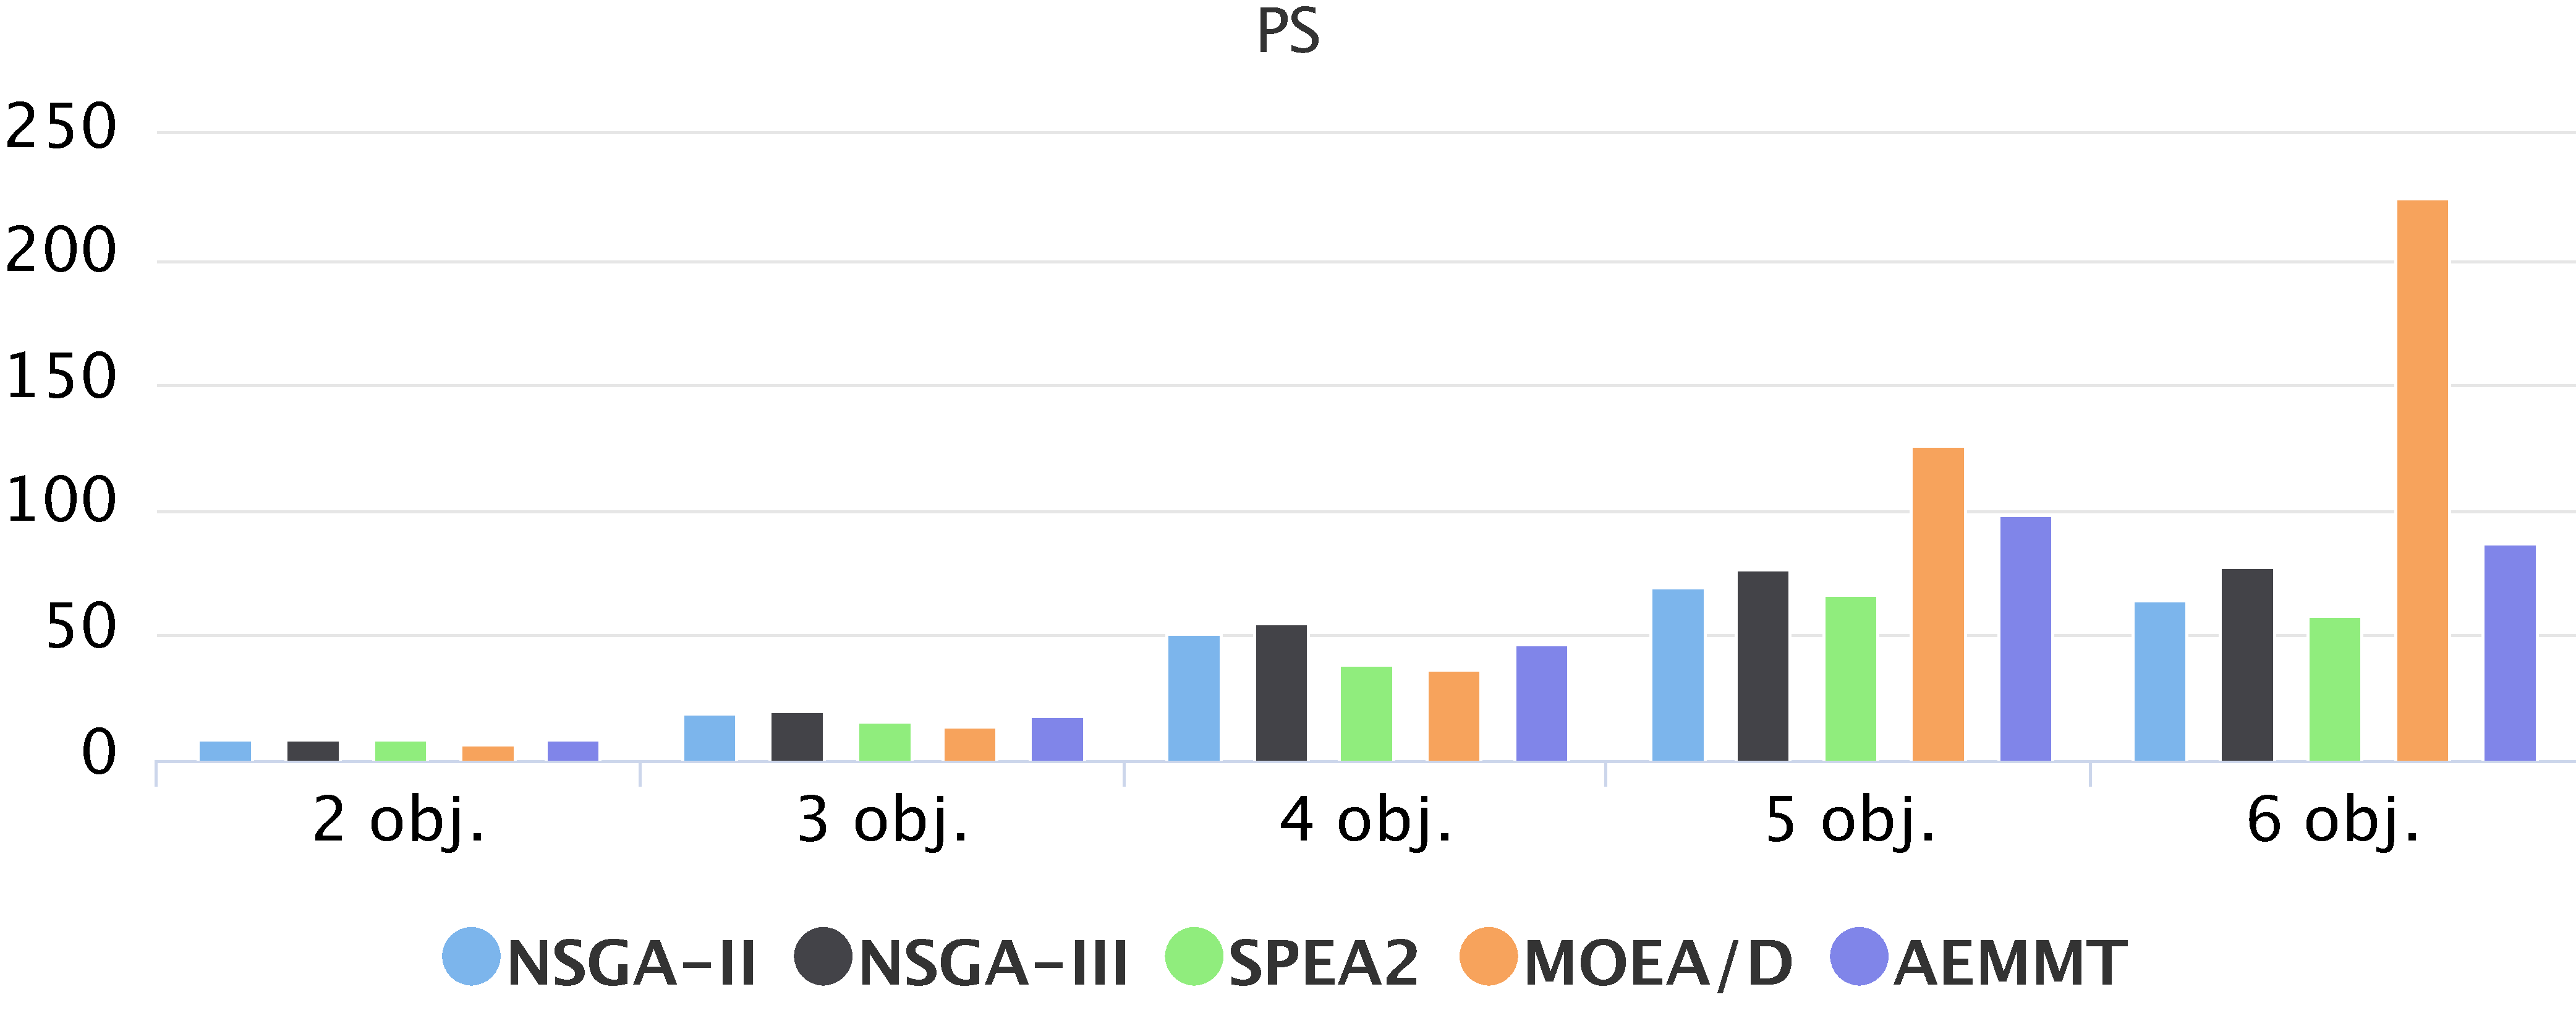
\includegraphics[width=1\textwidth]{cap_experimentos/figs/etapa1/ps-mrp-todos}
\end{figure*}

Afim de fazer uma análise geral do PRM, na figura \ref{fig_exp1_prm_todos}, todos os cenários (redes 1, 2 e 3) são combinados num único gráfico através de uma média aritmética dos resultados. Observa-se que, apesar de ser esperado que o NSGA-II e o SPEA2 fossem os melhores métodos para poucos objetivos, na verdade, o NSGA-III foi o algoritmo que obteve melhor resultado para problemas com, 2, 3 e 4 objetivos. O NSGA-II também produz bons resultados para problemas com 2 e 3 objetivos, mas o SPEA2 apresenta um $GD$ relativamente ruim. Considerando problemas de 5 e 6 objetivos, a escolha do algoritmo dependerá do intuito da busca, se é preferível uma maior quantidade de soluções, o MOEA/D é mais indicado, caso contrário, se um menor erro é preferível, então o AEMMT é a melhor opção.

Considerando ambos os problemas, PMM e PRM, os algoritmos NSGA-II, SPEA2 e NSGA-III são os que geram melhores resultados para problemas com poucos objetivos. A performance dos algoritmos clássicos (NSGA-II e SPEA2) cai consideravelmente a medida que se aumenta o número de objetivos, enquanto o desempenho dos métodos AEMMT e MOEA/D melhora a partir de quatro objetivos, tornando-nos os mais indicados para problemas \textit{many-objectives}.

Uma outra observação que pôde ser feita a partir dos experimentos nesta etapa é que o AEMMT perde apenas em $PS$ para o MOEA/D. Uma das características do AEMMT é a limitação no tamanho do arquivo, por isso surge a dúvida: se não houvesse um limite, seria possível que o AEMMT obtivesse um melhor resultado em todas as métricas? Pensando nisso, executou-se os mesmos testes para uma variação do AEMMT (AEMMT-F), onde o limite não foi aplicado. Na maioria dos resultados, o AEMMT-F apresentou erro maior que sua versão original, mas ainda sim $ER$ e $PS$ melhores que o MOEA/D. Dessa forma, através de um teste de hipótese z-teste com 0,1\% de significância ($\alpha = 0.1$), confirmou-se a superioridade do AEMMT-F em relação ao MOEA/D nos cenários com 5 e 6 objetivos.

\section{Etapa 2: MACO/D}
\label{section_experimentos_etapa2}

O algoritmo responsável pela construção das soluções do PRM no MACO/D foi concebido de acordo com os experimentos realizados nesta etapa. O mesmo processo não foi realizado para o PMM, pois já havia um modelo bem conceituado que funcionava bem com o algoritmo MACO/D. Além disso, aproveitou-se esse conjunto de experimentos para variar aspectos sobre a atualização de feromônios e parâmetros de entrada no ACO, resultando em particularidades do algoritmo descrito no capítulo \ref{chapter_macod}.

Como visto na seção \ref{section_estrategias_prm_aco}, foram estudadas quatro estratégias para se construir soluções no PRM. Primeiramente, foram implementados os dois algoritmos mais simples: estratégia 1 (formiga única) e 2 (múltiplas formigas). Infelizmente ambos os métodos não produziram resultados satisfatórios no problema do roteamento multicast multiobjetivo. Portanto, com a finalidade de se obter um problema mais simples e testar de maneira isolada o processo de construção da solução, decidiu-se elaborar um cenário do PRM com um único objetivo. As estratégias de construção da solução são apresentadas, em resumo, a seguir. Consulte a seção \ref{section_estrategias_prm_aco} para mais detalhes.

\begin{enumerate}
	\item Formiga única: o espaço de busca é explorado de forma aleatória, mas sempre considerando apenas a vizinhança da posição atual da formiga.
	\item Múltiplas formigas: uma formiga para cada destino. Une-se os caminhos produzidos por cada agente em uma árvore.
	\item Formiga com super-posição: uma formiga explora o espaço de busca de forma aleatória, mas pode estar em vários nós ao mesmo tempo, excluindo o problema de localidade na busca.
	\item Formigas invertidas: uma formiga para cada destino, mas ao invés de percorrerem o caminho da raiz ao destino, fazem o contrário, partem do destino e tentam encontrar a raiz.
\end{enumerate}

O problema mono-objetivo criado consiste em minimizar o valor de $custo * delay$ de uma árvore, portanto, quanto menor esse valor, melhor a árvore obtida. As quatro estratégias testadas são aquelas mencionadas na seção \ref{section_estrategias_prm_aco}. Além dos quatro algoritmos, é incluído um resultado novo, obtido a partir de uma modificação do algoritmo de Prim \cite{Prim1957}, para servir como referência de uma boa solução possível de ser encontrada. Cada estratégia foi executada cinco vezes e a tabela \ref{tab_exp2_estrategias} mostra o resultado da melhor execução de cada estratégia.

\begin{table}[!htbp]
	\centering
	\caption{Resultados para as estratégias de construção de solução do PRM}
	\label{tab_exp2_estrategias}
	\begin{tabular}{rrrr}
		Estratégia & Rede & Resultado   & Tempo (s)    \\ \hline
		Prim       & $R_1$   & 3.285714286 & 0.021     \\
		1          & $R_1$   & 3.047619048 & 2.496     \\
		2          & $R_1$   & 3.031746032 & 5.94      \\
		\rowcolor{table-green} 
		3          & $R_1$   & 3.007936508 & 3.88      \\
		\rowcolor{table-green} 
		4          & $R_1$   & 3.007936508 & 3.16      \\ \hline
		Prim       & $R_2$   & 3.134920635 & 0.016     \\
		1          & $R_2$   & 3.341269841 & 4.947     \\
		2          & $R_2$   & 3.261904762 & 13.22     \\
		\rowcolor{table-green} 
		3          & $R_2$   & 3.134920635 & 10.694    \\
		4          & $R_2$   & 3.301587302 & 5.549     \\ \hline
		Prim       & $R_3$   & 7.968253968 & 0.024     \\
		1          & $R_3$   & 8.134920635 & 4.212     \\
		2          & $R_3$   & 8.238095238 & 25.606    \\
		\rowcolor{table-green} 
		3          & $R_3$   & 7.484126984 & 9.821     \\
		4          & $R_3$   & 8.111111111 & 6.939     \\ \hline
		Prim       & $R_4$   & 1.801587302 & 0.025     \\
		1          & $R_4$   & 2.341269841 & 4.715     \\
		2          & $R_4$   & 2.325396825 & 12.471    \\
		\rowcolor{table-green} 
		3          & $R_4$   & 1.857142857 & 11.015    \\
		4          & $R_4$   & 1.976190476 & 4.935     \\ \hline
		Prim       & $R_5$   & 6.341269841 & 0.015     \\
		1          & $R_5$   & 6.126984127 & 6.87      \\
		2          & $R_5$   & 6.333333333 & 17.38     \\
		\rowcolor{table-green} 
		3          & $R_5$   & 5.857142857 & 14.767    \\
		\rowcolor{table-green} 
		4          & $R_5$   & 5.857142857 & 8.423     \\ \hline
	\end{tabular}
\end{table}

Na tabela \ref{tab_exp2_estrategias}, a coluna ``resultado'' representa a soma dos valores de $custo * delay$ das arestas da árvore obtida como solução, ou seja, quanto menor esse valor, melhor a solução obtida. Dessa forma, a estratégia número 3, que usa a ideia de formiga com super-posição, obteve melhor performance. Em termos de tempo, ela infelizmente leva mais tempo que a maioria das demais. Por essa razão propõe-se a ideia de amostragem explicada na seção \ref{section_estrategias_prm_aco}. Ao construir a solução, ao invés de se utilizar a totalidade do conjunto de exploração, toma-se uma amostra desse. Em nossos testes para o PRM, a amostragem é sempre de 10 elementos. A tabela \ref{tab_exp2_amostragem} mostra uma comparação da estratégia 3 com e sem a amostragem.

\begin{table}[!htbp]
	\centering
	\caption{Comparação entre da estratégia 3 na técnica de amostragem}
	\label{tab_exp2_amostragem}
	\begin{tabular}{rrrr}
		Amostragem    & Rede & Resultado   & Tempo (s) \\ \hline
		s/ amostragem & $R_1$    & 3.007936508 & 3.88      \\
		\rowcolor{table-green}
		c/ amostragem & $R_1$    & 3.007936508 & 3.41      \\ \hline
		s/ amostragem & $R_2$    & 3.134920635 & 10.694    \\
		\rowcolor{table-green}
		c/ amostragem & $R_2$    & 3.134920635 & 7.602     \\ \hline
		s/ amostragem & $R_3$    & 7.484126984 & 9.821     \\
		\rowcolor{table-green}
		c/ amostragem & $R_3$    & 7.484126984 & 7.26      \\ \hline
		s/ amostragem & $R_4$    & 1.857142857 & 11.015    \\
		\rowcolor{table-green}
		c/ amostragem & $R_4$    & 1.785714286 & 7.28      \\ \hline
		s/ amostragem & $R_5$    & 5.857142857 & 14.767    \\
		\rowcolor{table-green}
		c/ amostragem & $R_5$    & 5.76984127  & 10.037    \\ \hline
	\end{tabular}
\end{table}

Como pode ser observado na tabela \ref{tab_exp2_amostragem}, a amostragem não só diminuiu o tempo do algoritmo como também melhorou o resultado. A melhora na qualidade da solução pode ser atribuída ao maior grau de aleatoriedade dada ao algoritmo, similar ao que acontece nos algoritmos genéticos quando se lança mão de operações como a mutação ou seleções por torneio.

Ao implementar a estratégia 1 (uma formiga e super-posição) com amostragem no PRM many-objetive, percebeu-se que o AEMMD conseguia resultados muitos superiores (tabela \ref{tab_exp2_macod_simples}) ao novo algoritmo. A fim de reduzir essa diferença, propôs-se as seguintes mudanças para o MACO/D:

\begin{itemize}
	\item Depósito de feromônio baseado na qualidade da aresta (ou do item, no caso do PMM): num problema multi-objetivo, ao depositar feromônios sobre as arestas correspondentes às soluções não-dominadas, sempre deposita-se a mesma quantidade independente da solução e da aresta, pois, segundo a relação de não-dominância, ambas opções são igualmente boas. Esta proposta muda esse conceito ligando a quantidade de feromônios depositados à qualidade da aresta, i.e., a quantidade passa a ser inversamente proporcional à soma dos pesos da aresta (considerando um problema de minimização).
	\item Dinamização do parâmetro de entrada $\beta$: $\beta$ é o valor que controla a importância da heurística ao calcular as probabilidades de cada aresta (ou item, no PMM) de fazer parte da solução. A proposta é diminuir um pouco a importância da heurística, dando maior peso à informação de feromônio sempre que, após uma iteração, não for encontrada uma nova solução. Assim que uma nova solução é encontrada, o valor de beta é reiniciado para o padrão.
\end{itemize}

Tomando como referência o problema $P_6$, com seis objetivos, construiu-se a tabela \ref{tab_exp2_macod_simples} que mostra as diferenças entre os desempenhos dos algoritmos AEMMD, MACO/D antes das alterações no depósito de feromônios e do parâmetro $\beta$ (MACO/D-pré) e o algoritmo final proposto no capítulo \ref{chapter_macod} (MACO/D).

\begin{table}[!htbp]
	\centering
	\caption{Desempenho do AEMMD, MACO/D pré-alterações e MACO/D final}
	\label{tab_exp2_macod_simples}
	\begin{tabular}{rrrrr}
		Algoritmo  & Rede  & $ER$  & $GD$ & $PS$  \\ \hline
		AEMMD      & $R_1$ & 6.59  & 0.38 & 502.8 \\
		MACO/D-pré & $R_1$ & 18.42 & 0.30 & 337.6 \\
		MACO/D     & $R_1$ & 11.57 & 0.36 & 424.2 \\ \hline
		AEMMD      & $R_2$ & 7.58  & 0.49 & 296.6 \\
		MACO/D-pré & $R_2$ & 11.75 & 0.47 & 284.4 \\
		MACO/D     & $R_2$ & 11.18 & 0.37 & 300   \\ \hline
		AEMMD      & $R_3$ & 11.73 & 0.19 & 388.6 \\
		MACO/D-pré & $R_3$ & 36.47 & 0.16 & 206   \\
		MACO/D     & $R_3$ & 30.20 & 0.25 & 232.4 \\ \hline
		AEMMD      & $R_4$ & 35.88 & 0.17 & 234   \\
		MACO/D-pré & $R_4$ & 54.48 & 0.11 & 150.2 \\
		MACO/D     & $R_4$ & 50.57 & 0.15 & 186.6 \\ \hline
		AEMMD      & $R_5$ & 32.67 & 0.20 & 181.2 \\
		MACO/D-pré & $R_5$ & 32.95 & 0.22 & 168.6 \\
		MACO/D     & $R_5$ & 32.67 & 0.30 & 160.8
	\end{tabular}
\end{table}

Na tabela \ref{tab_exp2_macod_simples} pode-se observar que na maioria dos casos as duas alterações propostas melhoraram o resultado do MACO/D, portanto, o algoritmo final proposto inclui essas duas pequenas alterações. O AEMMD ainda apresenta melhores resultados, mas como será visto nas etapas 3 e 4 de experimentos, o MACO/D leva até 5 vezes menos tempo para executar.

\section{Etapa 3: AG's \textit{many-objectives} vs. MACO/D}
\label{section_experimentos_etapa3}

Na terceira etapa de experimentos descartam-se os AEMOs clássicos NSGA-II e SPEA2 e inclui-se o AEMMD e o MACO/D, algoritmo proposto neste trabalho. Uma nova métrica de desempenho é utilizada, o tempo, e as demais continuam sendo o erro ($ER$), a distância ($GD$) e o número de soluções corretas ($PS$). Assim como na etapa 1, o Pareto aproximado foi pré-calculado a partir de múltiplas execuções dos algoritmos e é apresentado na tabela \ref{table_exp3_paretos}. Enfim, os resultados (com exceção do tempo) foram obtidos através das médias entre 100 execuções dos 30 cenários descritos na lista a seguir. À medida de tempo considerou apenas 3 execuções de cada algoritmo em cada cenário.

\begin{itemize}
	\item PRM: 3 formulações de objetivos ($P_4$, $P_5$ e $P_6$) e 3 redes ($R_1$, $R_2$ e $R_3$). Tanto as formulações quanto às redes foram descritas na seção correspondente ao problema do roteamento multicast \ref{section_problemas_prm}.
	\item PMM: 3 formulações de objetivos (4 a 6) e 3 instâncias (30, 40 e 50 itens).
\end{itemize}


\begin{table}[!htbp]
	\centering
	\caption{Cardinalidade dos Paretos encontrados para a primeira etapa de experimentos}
	\label{table_exp3_paretos}
	\begin{tabular}{c|rrr|rrr}
		& \multicolumn{3}{c|}{\textbf{PRM}} & \multicolumn{3}{c}{\textbf{PMM}} \\ \hline
		Objetivos & R1         & R2       & R3        & 30 itens  & 40 itens & 50 itens \\ \hline
		4         & 122        & 553       & 1349        & 425       & 1199      & 1012    \\
		5         & 75        & 372      & 712       & 1769      & 3862     & 5467   \\
		6         & 60       & 660      & 1283      & 5828      & 6491   & 55471   \\ \hline
	\end{tabular}
\end{table}

A tabela \ref{table_exp3_parametros} apresenta os parâmetros dos algoritmos utilizados neste experimento. Note que o número de gerações (marcado com asterisco) deve ser multiplicado pelo tamanho da população no AEMMT e AEMMD devido ao fato de realizarem apenas um crossover por geração.

\begin{table}[!htbp]
	\caption{Parâmetros utilizados para o PRM e o PMM na etapa 3 de experimentos.}
	\label{table_exp3_parametros}
	\begin{center}
		\begin{tabular}{c|r|r}
			\textbf{Parâmetro} & \textbf{PRM} &  \textbf{PMM} \\ %\hline
			\hline
			Tamanho da população               &    90 &      150 \\ %\hline
			Número de gerações*        &   100 &      100 \\ %\hline
			Taxa de crossover                & 100\% &    100\% \\ %\hline
			Taxa de mutação                 &  20\% &      5\% \\ %\hline
			Tamanho da vizinhança (MOEA/D)    &    10 &       10 \\ %\hline
			Tamanho das tabelas (MEAMT)   &    30 &       50 \\ %\hline
			Tamanho da tabela de dominância (MEAMT) &    90 &      150 \\ %\hline
			Número de divisões (NSGA-III)&     8 &        8 \\ %\hline
			$\alpha, \beta, \rho$ (MACO/D)& 1, 2, 0.3 & 1, 4.3, 0.3 \\ %\hline
			Intervalo de valores para os feromônios (MACO/D)& [0.1, 0.9] & [0.1, 0.9] \\ %\hline
			Tamanho das amostras (MACO/D)& 10 &25\% of the number of items \\  %\hline
			Tamanho do grupo de estruturas ativas (MACO/D)& 5 & 5 \\
			\hline
		\end{tabular}
	\end{center}
\end{table}

As figuras \ref{fig_exp3_pmm_30}, \ref{fig_exp3_pmm_40} e \ref{fig_exp3_pmm_50} mostram respectivamente os resultados para o PMM de 30, 40 e 50 itens. As figuras \ref{fig_exp3_prm_r1}, \ref{fig_exp3_prm_r2} e \ref{fig_exp3_prm_r3} revelam respectivamente os resultados para o PRM aplicado às redes $R_1$, $R_2$ e $R_3$. Uma análise conjunta, com uma média entre as três instâncias de cada problema é apresenta nas figuras \ref{fig_exp3_prm_todos} (PRM) e \ref{fig_exp3_pmm_todos} (PMM).

\begin{figure*}[!htbp]
	\caption{Etapa 3: resultados para o PMM com 30 itens}
	\label{fig_exp3_pmm_30}
	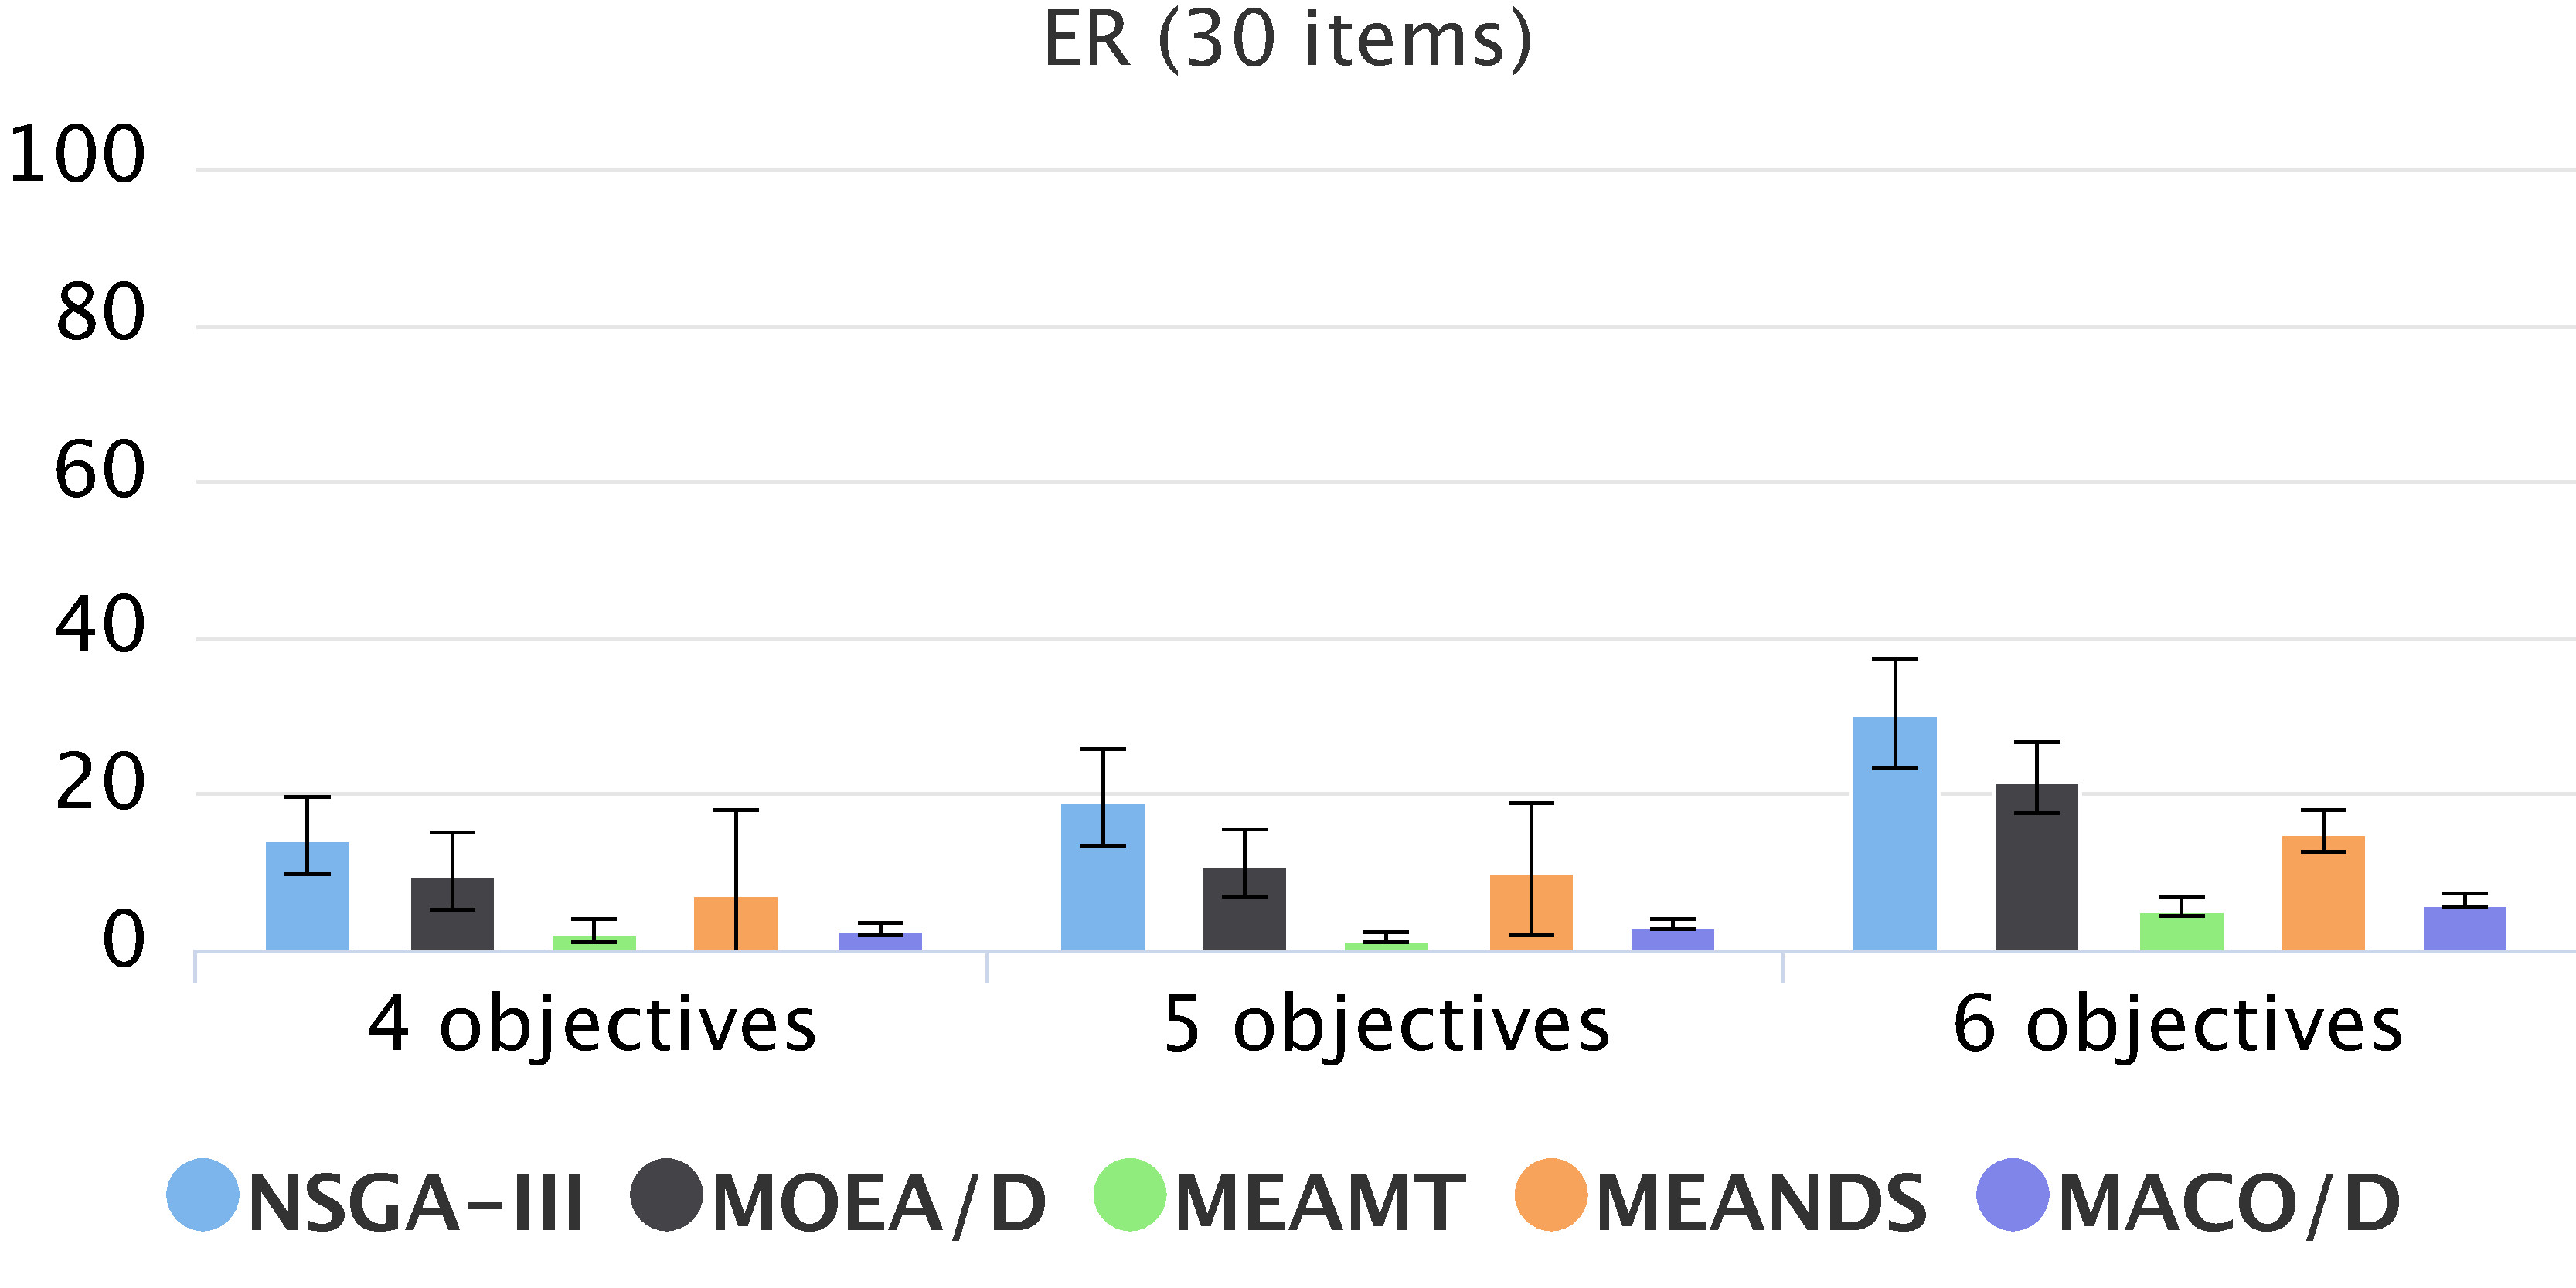
\includegraphics[width=0.5\textwidth]{cap_experimentos/figs/etapa3/er-mkp-30}
	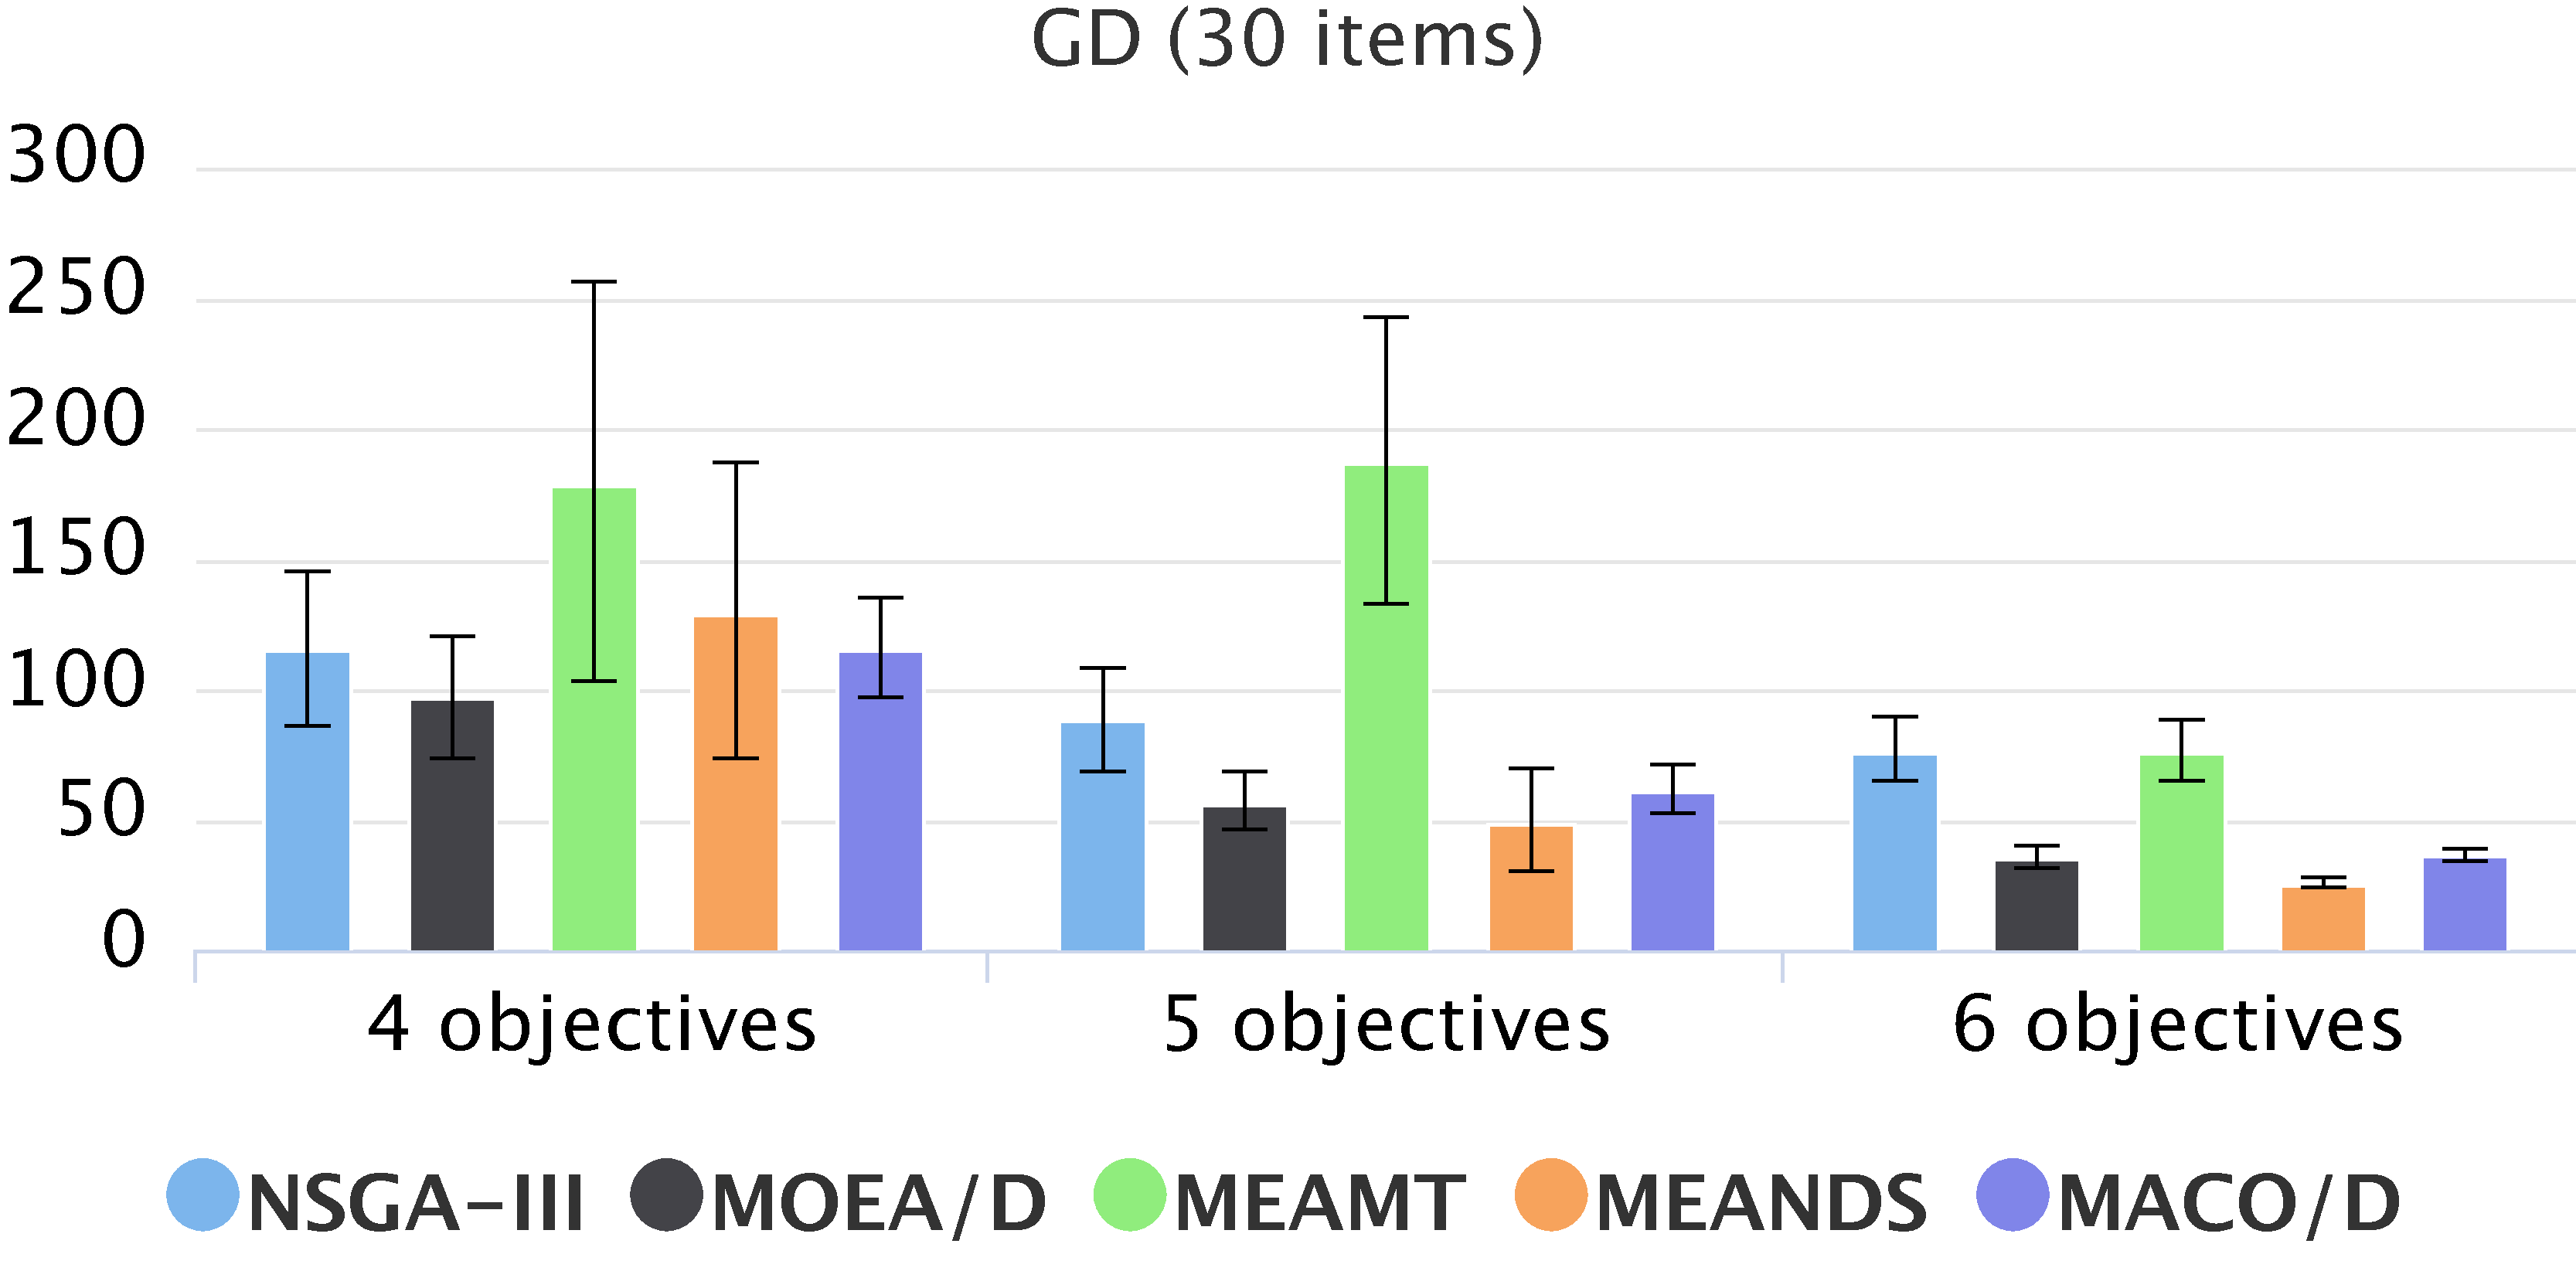
\includegraphics[width=0.5\textwidth]{cap_experimentos/figs/etapa3/gd-mkp-30}
	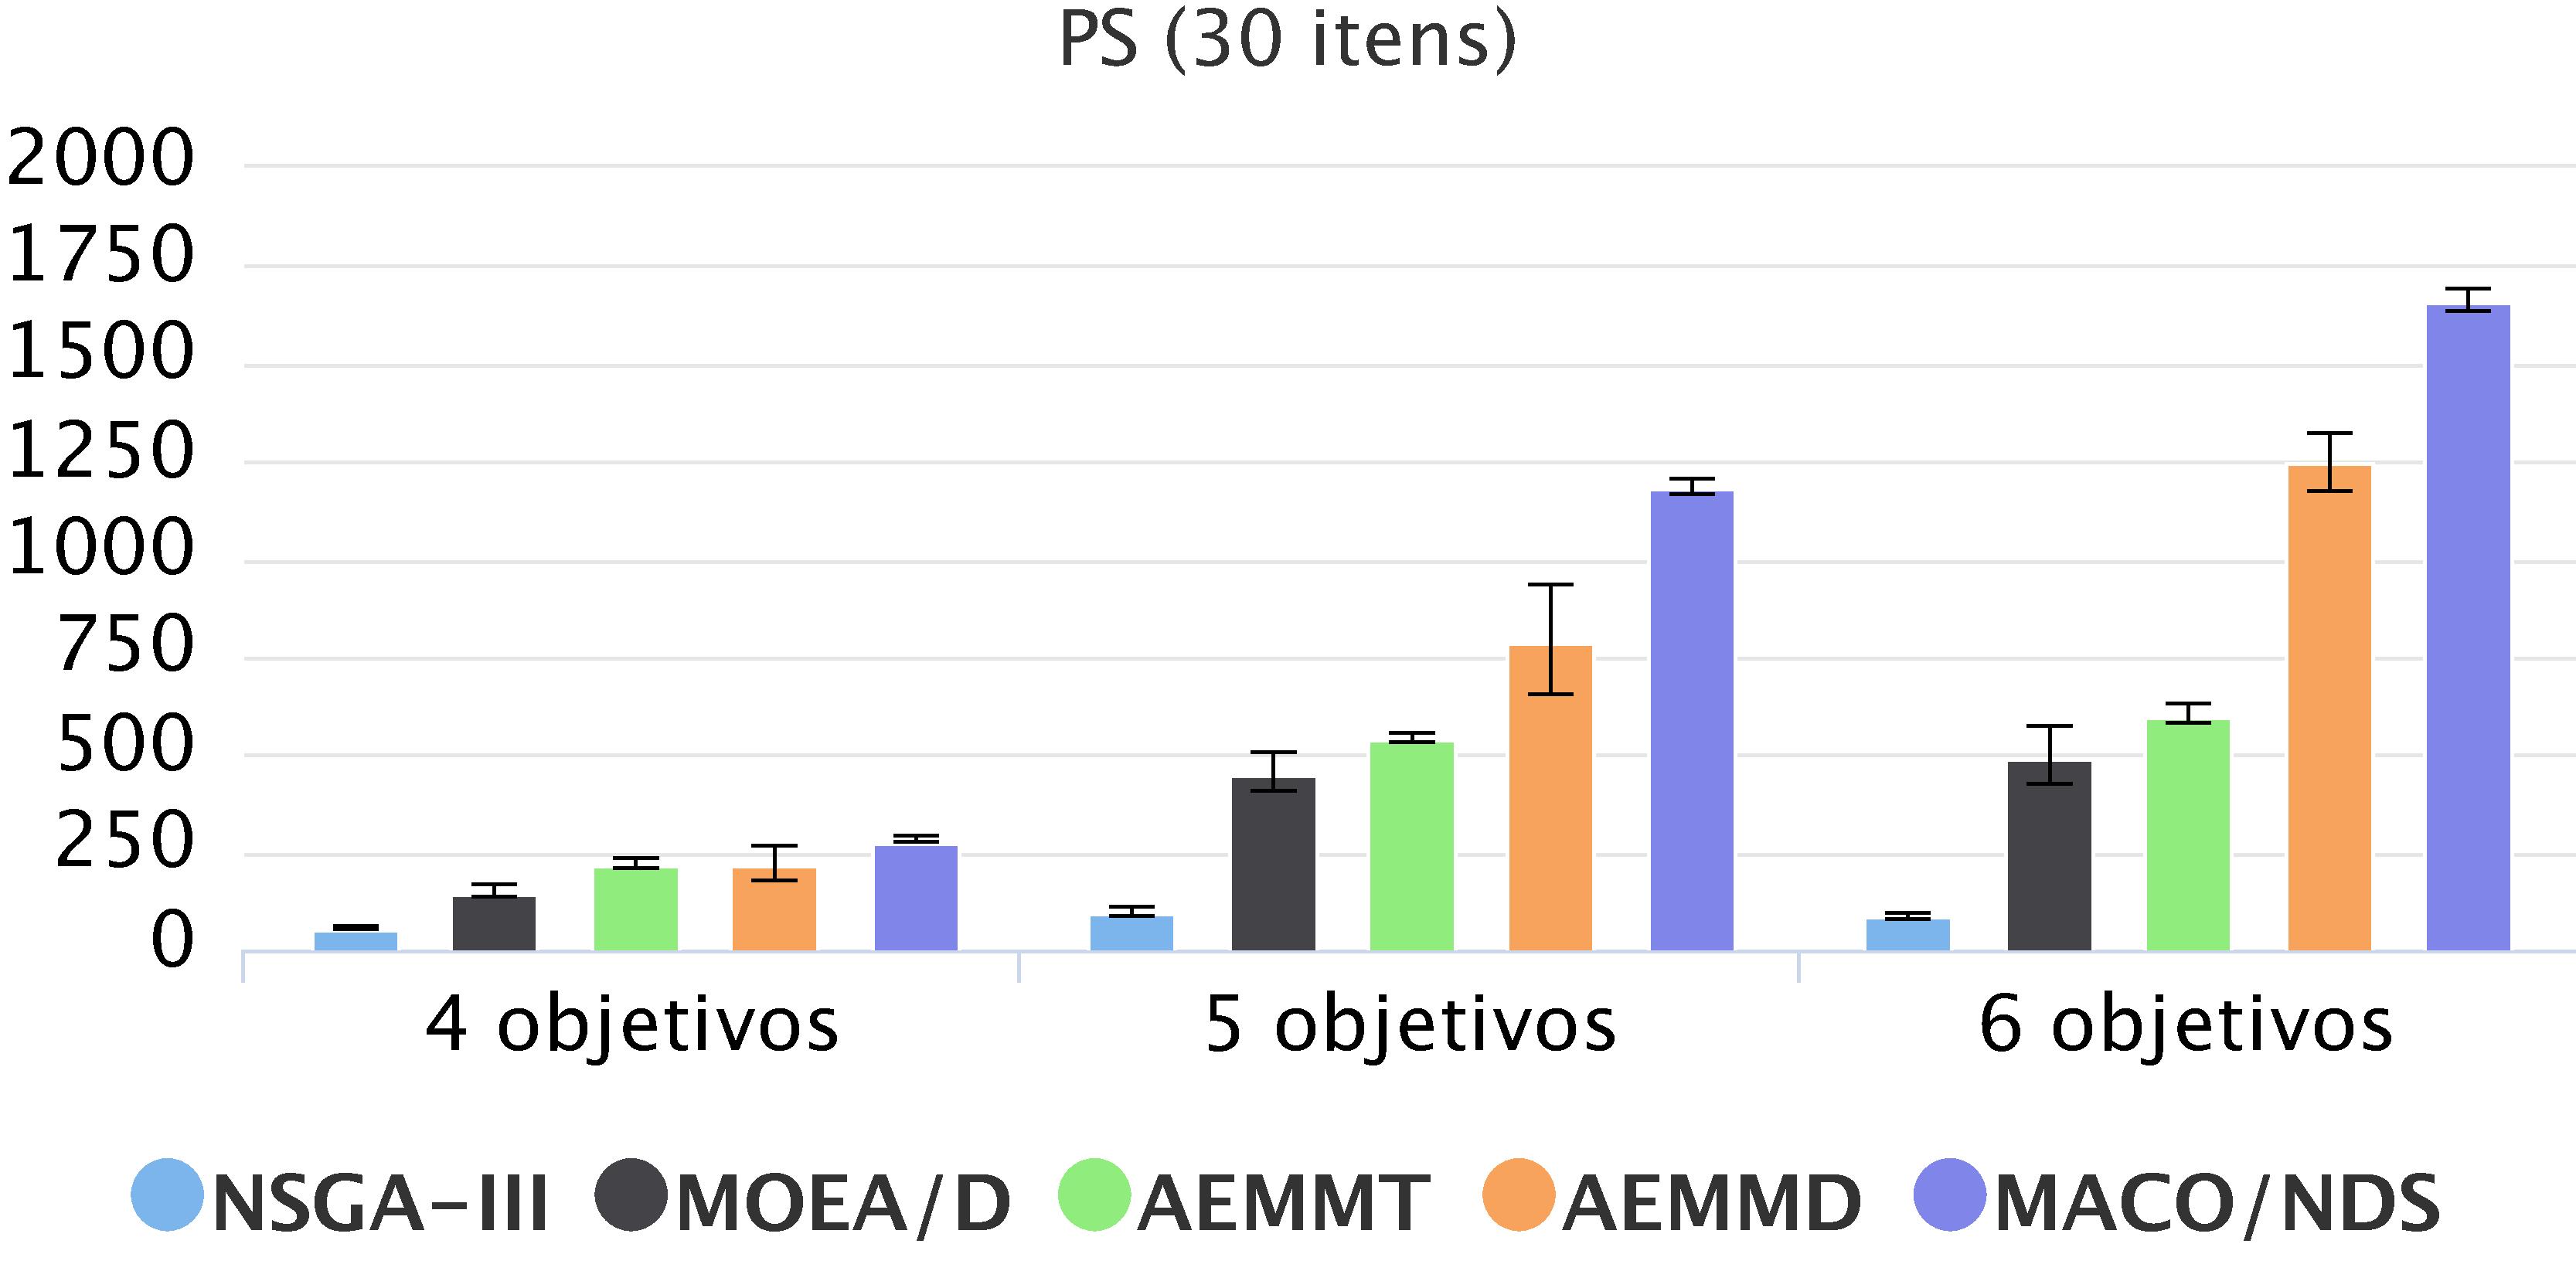
\includegraphics[width=0.5\textwidth]{cap_experimentos/figs/etapa3/ps-mkp-30}
	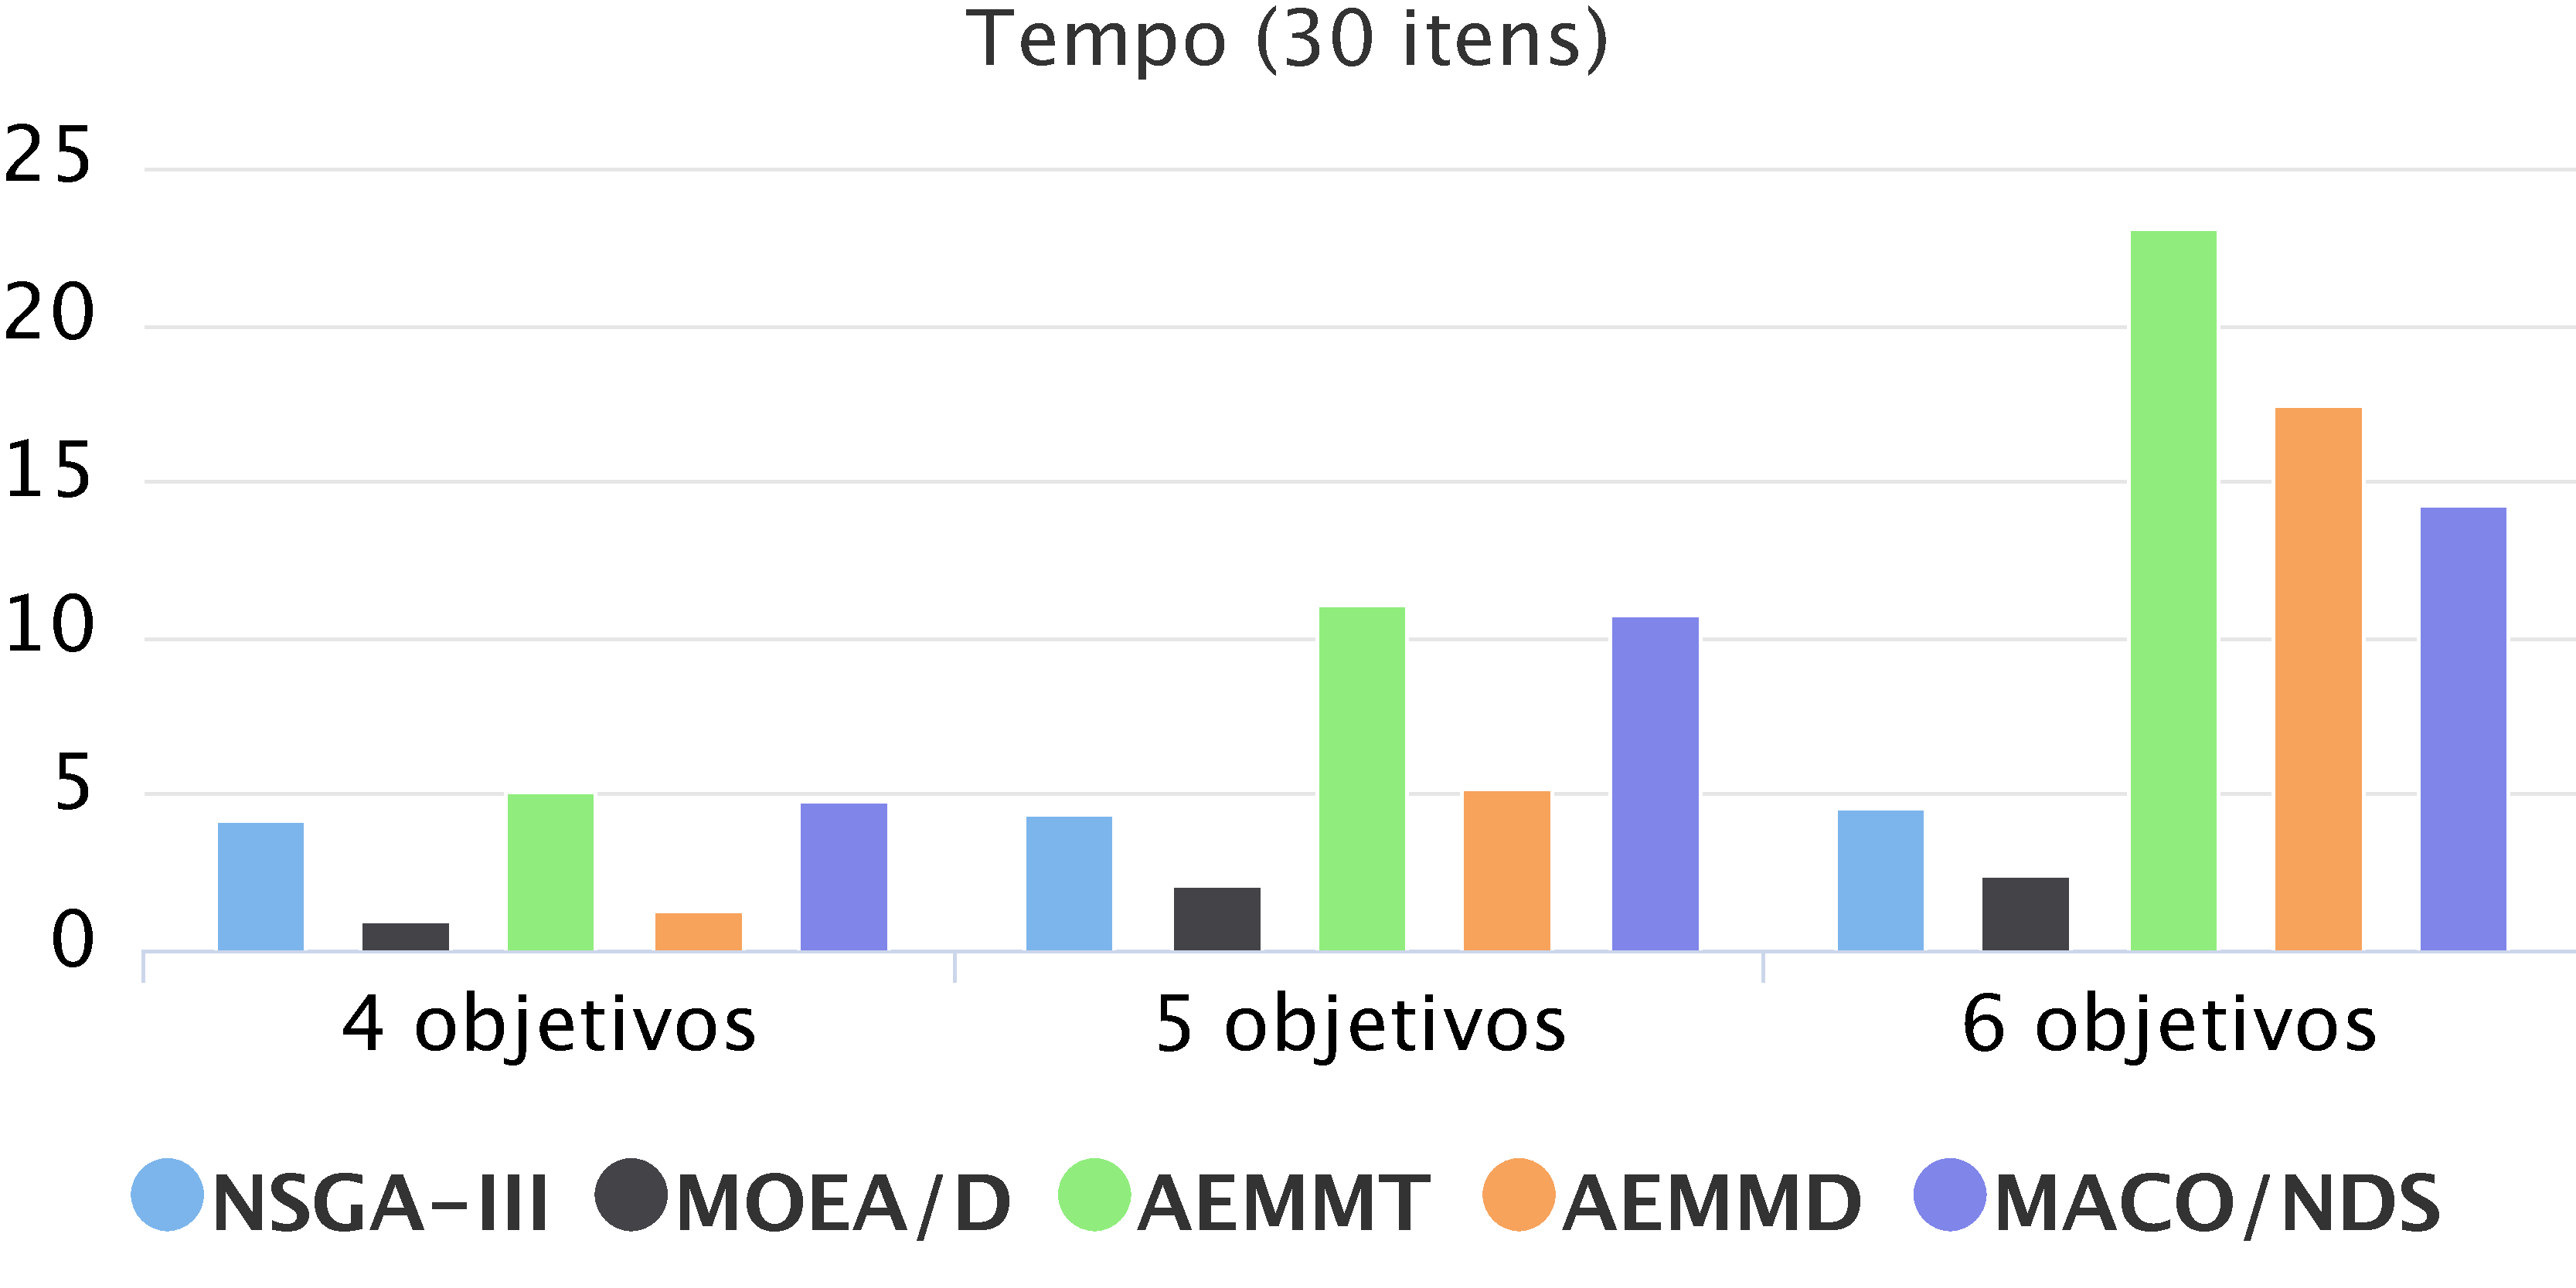
\includegraphics[width=0.5\textwidth]{cap_experimentos/figs/etapa3/time-mkp-30}
\end{figure*}

No problema da mochila mais simples, de 30 itens (figura \ref{fig_exp3_pmm_30}), o AEMMT apresenta a menor taxa de erro dentre os algoritmos \textit{many-objectives}, em segundo lugar está o MACO/D e em terceiro o AEMMD. Com relação ao $GD$, com 4 objetivos, os melhores resultados são encontrados pelo MOEA/D seguido pelo MACO/D. O Em 5 e 6 objetivos, o AEMMD produz o menor $GD$, e o MACO/D, bem próximo, aparece em segundo lugar. Na métrica $PS$, o MACO/D é melhor que os demais em todos as formulações de objetivo, seguido, em ordem pelo AEMMD, AEMMT, MOEA/D e NSGA-III. Destre esses algoritmos, o único com um limite fixo no tamanho do Pareto é o NSGA-III, portanto, é esperado que possua um valor de $PS$ menor. Quanto ao tempo, o MOEA/D é o algoritmo mais rápido dentre os 5.

\begin{figure*}[!htbp]
	\caption{Etapa 3: resultados para o PMM com 40 itens}
	\label{fig_exp3_pmm_40}
	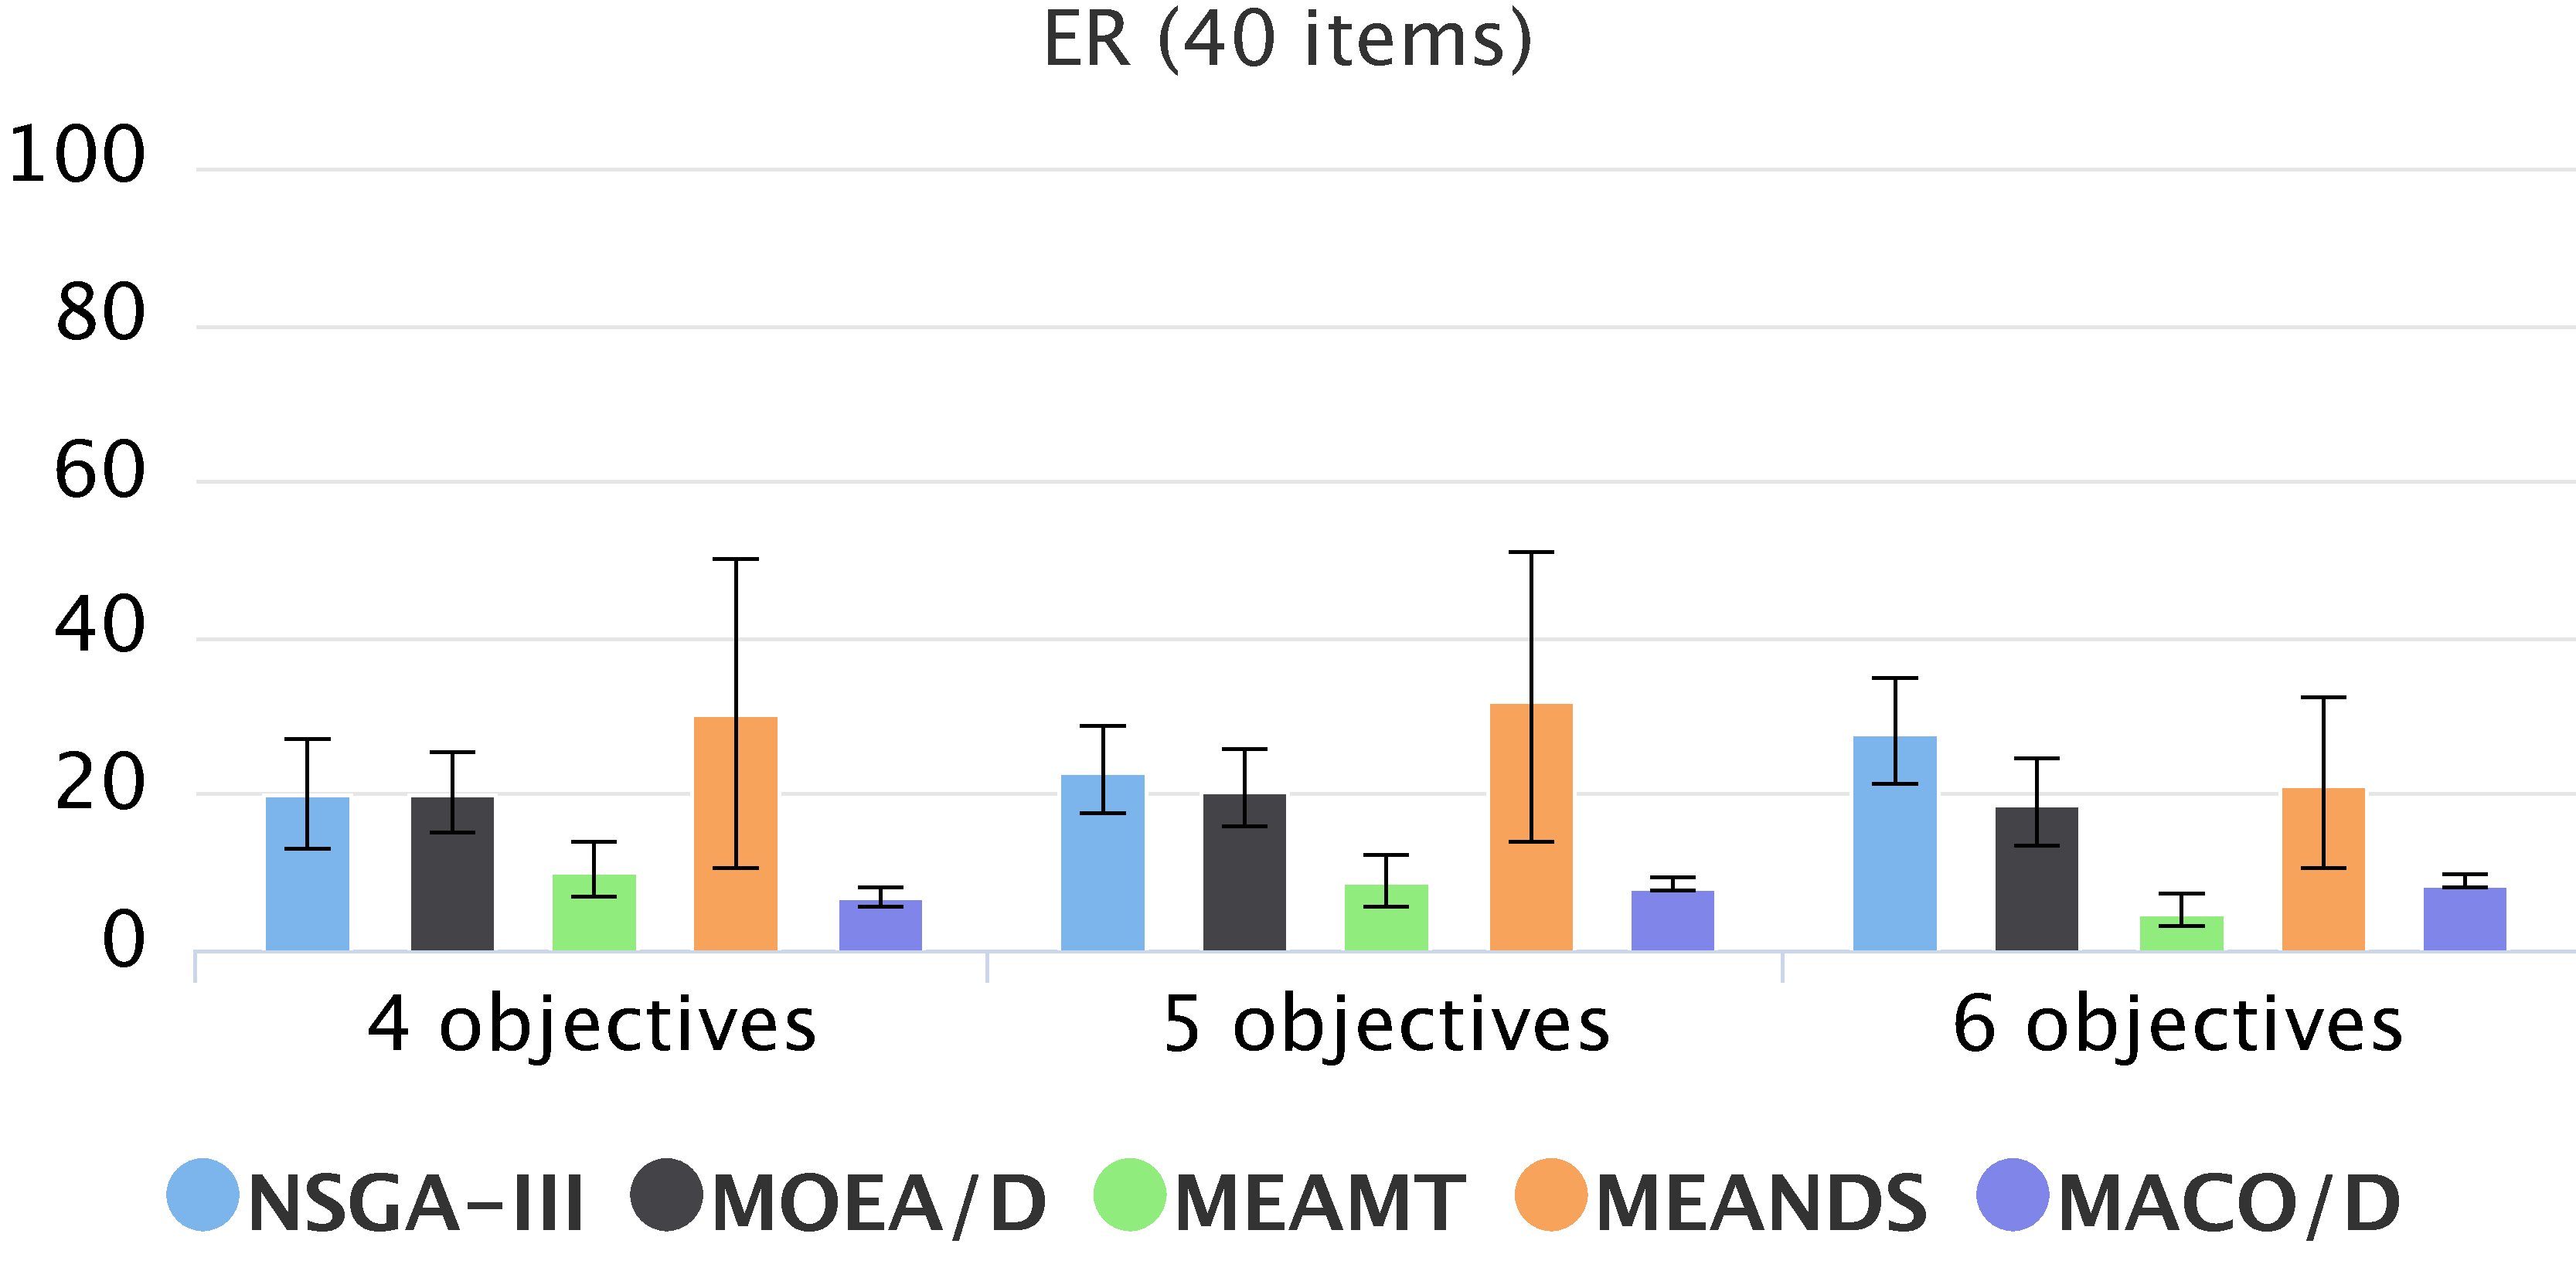
\includegraphics[width=0.5\textwidth]{cap_experimentos/figs/etapa3/er-mkp-40}
	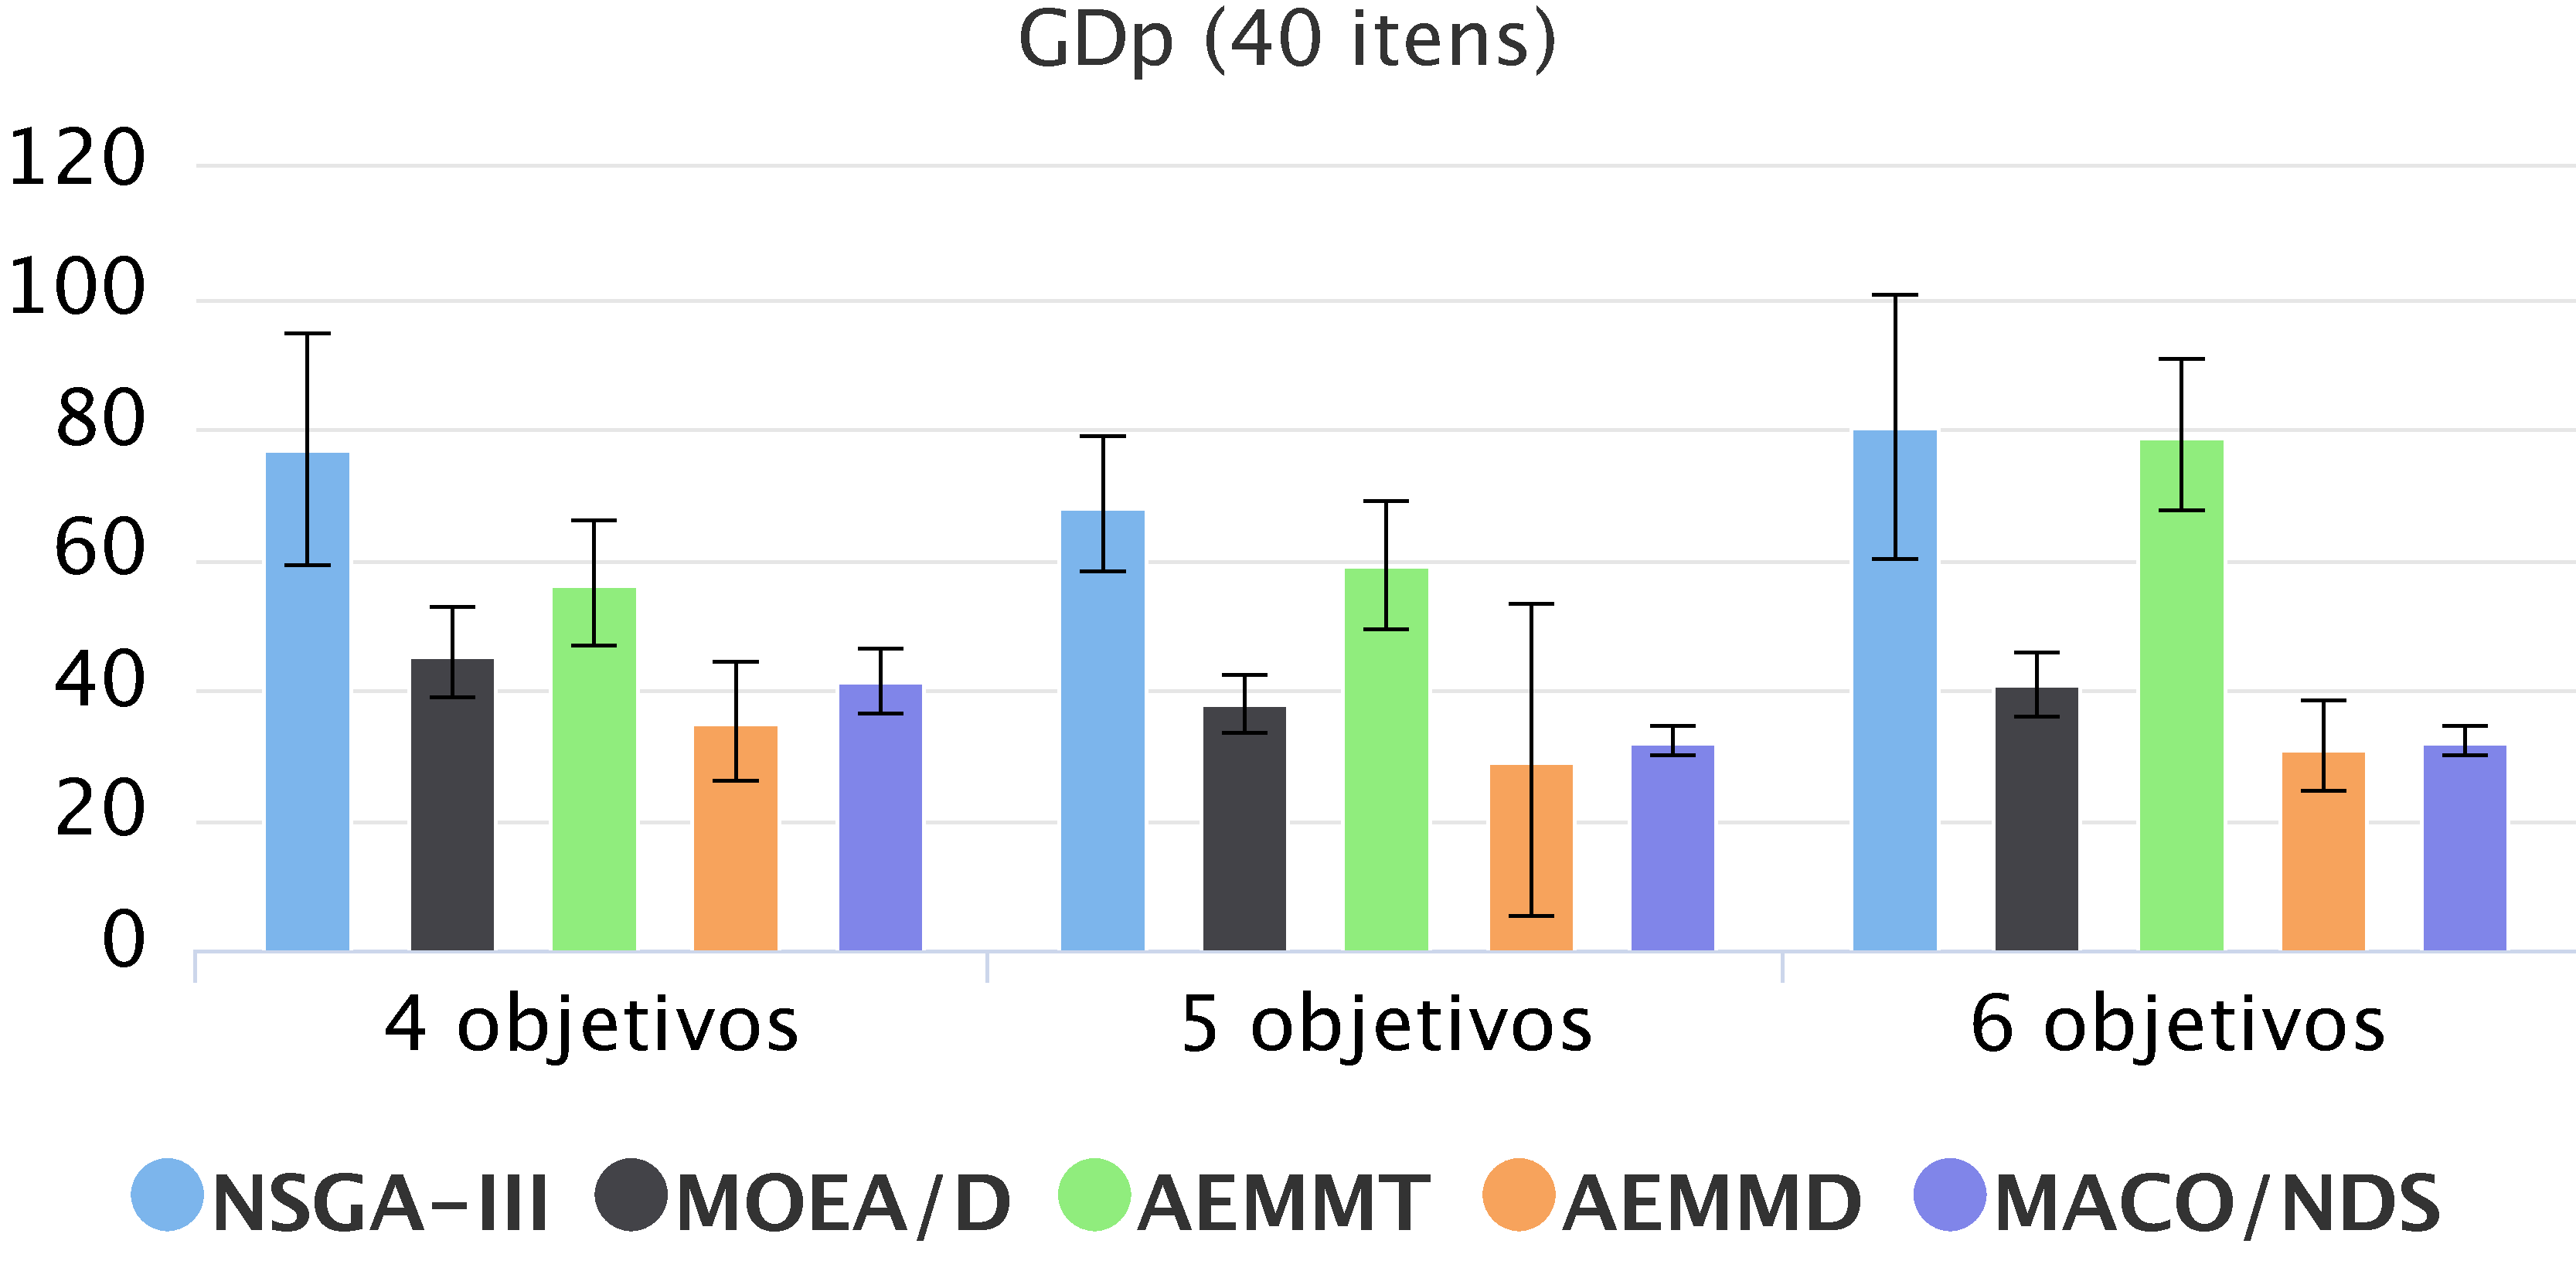
\includegraphics[width=0.5\textwidth]{cap_experimentos/figs/etapa3/gd-mkp-40}
	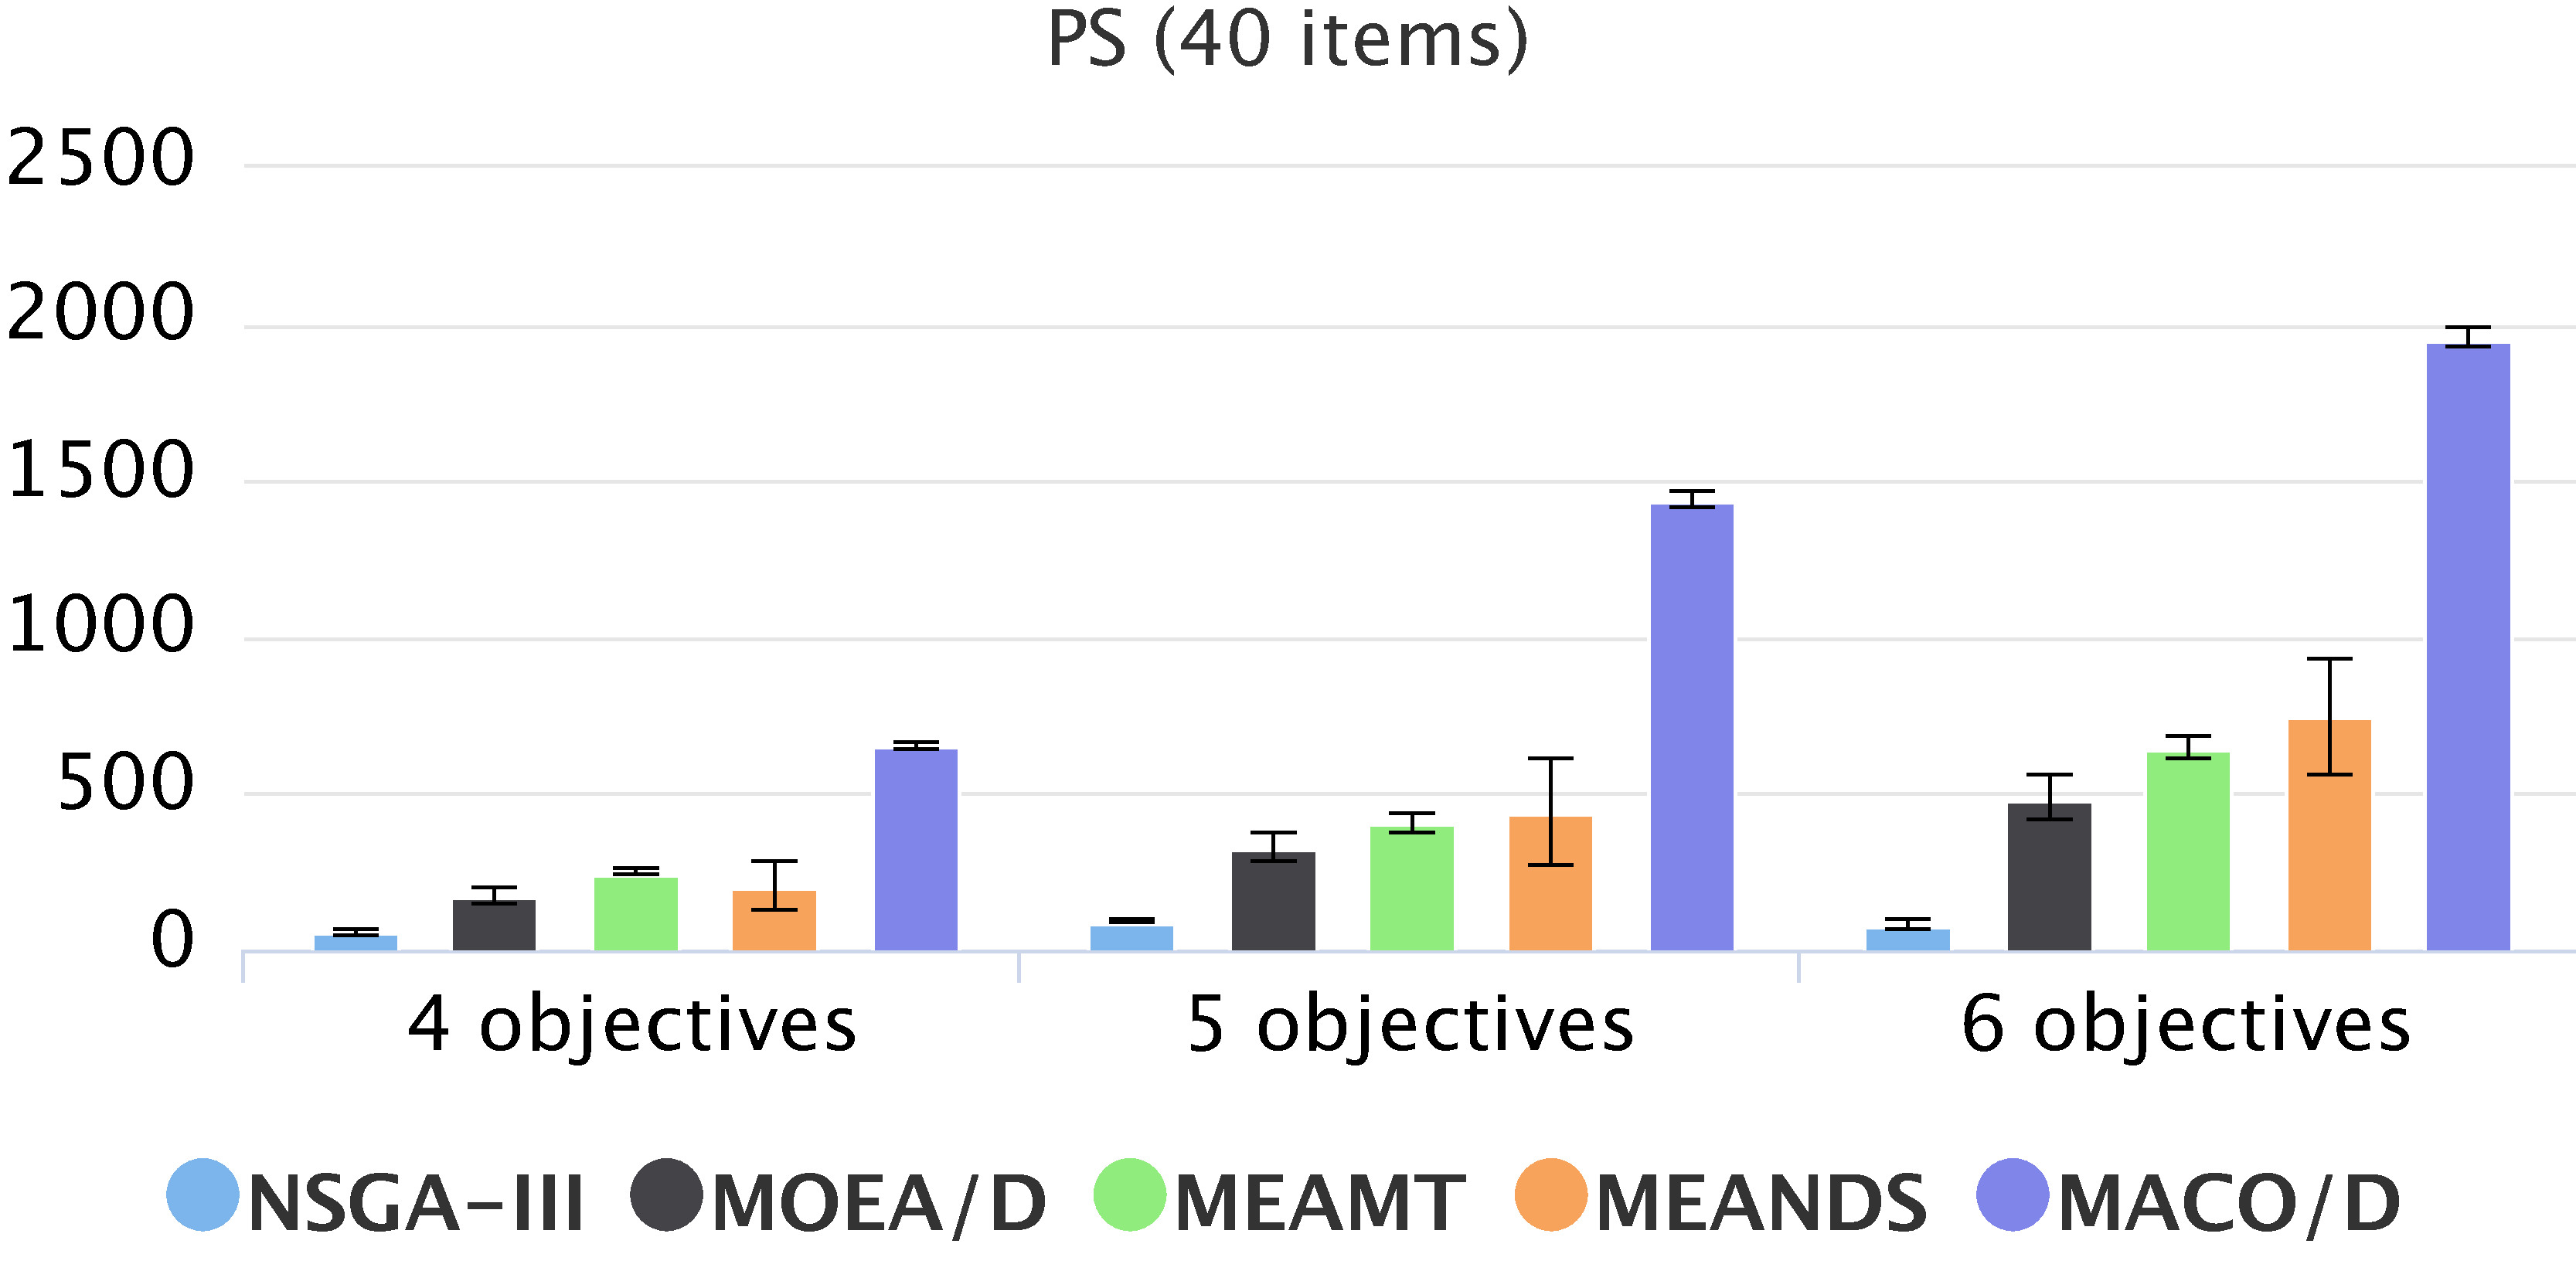
\includegraphics[width=0.5\textwidth]{cap_experimentos/figs/etapa3/ps-mkp-40}
	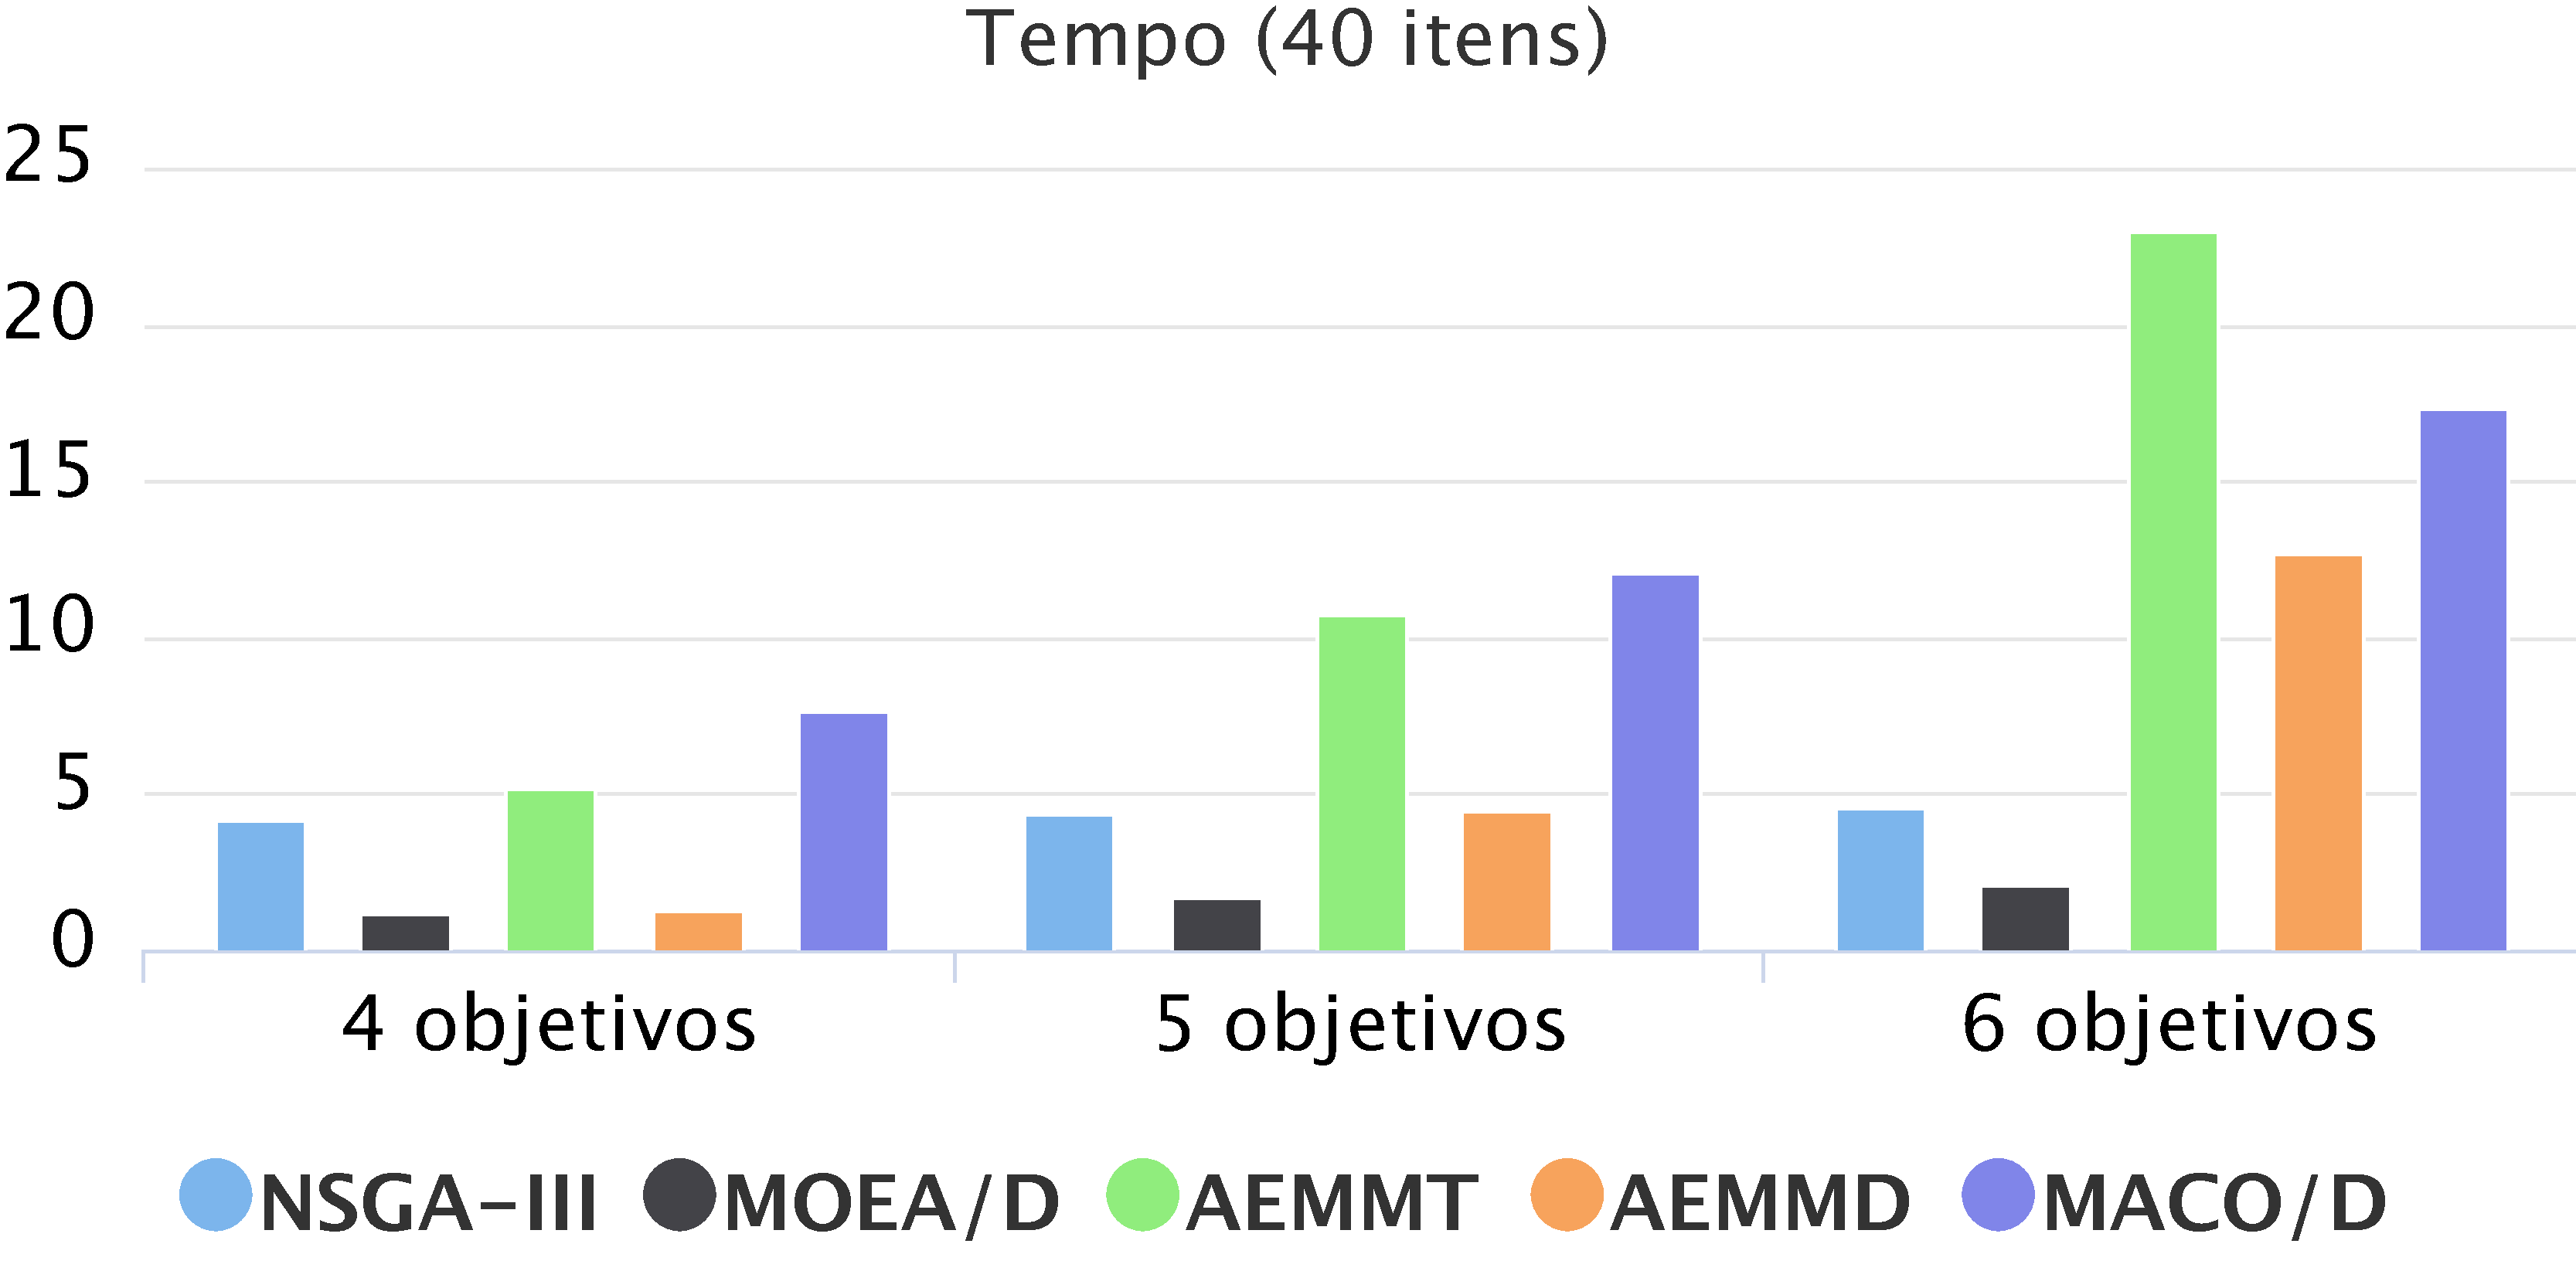
\includegraphics[width=0.5\textwidth]{cap_experimentos/figs/etapa3/time-mkp-40}
\end{figure*}

O PMM de 40 itens é analisado na figura \ref{fig_exp3_pmm_40}. O AEMMT e o MACO/D apresentam a menor taxa de erro, sendo que o MACO/D é melhor para 4 e 5 objetivos, enquanto o AEMMT obtém o melhor resultado para 6 objetivos. Os melhores valores de $GD$ foram encontrados pelo AEMMD e MACO/D, sendo que o AEMMD é um pouco melhor no problema com 4 objetivos. Uma característica negativa do AEMMD em relação ao MACO/D no que se refere ao $GD$ é sua alta variação nos resultados, o que diz que algumas execuções produz soluções muito próximas do Pareto enquanto outras nem tanto. A respeito do tamanho dos Paretos encontrados, novamente o MACO/D lidera independente da formulação de objetivos. O MOEA/D é o algoritmo mais rápido, enquanto o AEMMT e o MACO/D são os mais lentos.

\begin{figure*}[!htbp]
	\caption{Etapa 3: resultados para o PMM com 50 itens}
	\label{fig_exp3_pmm_50}
	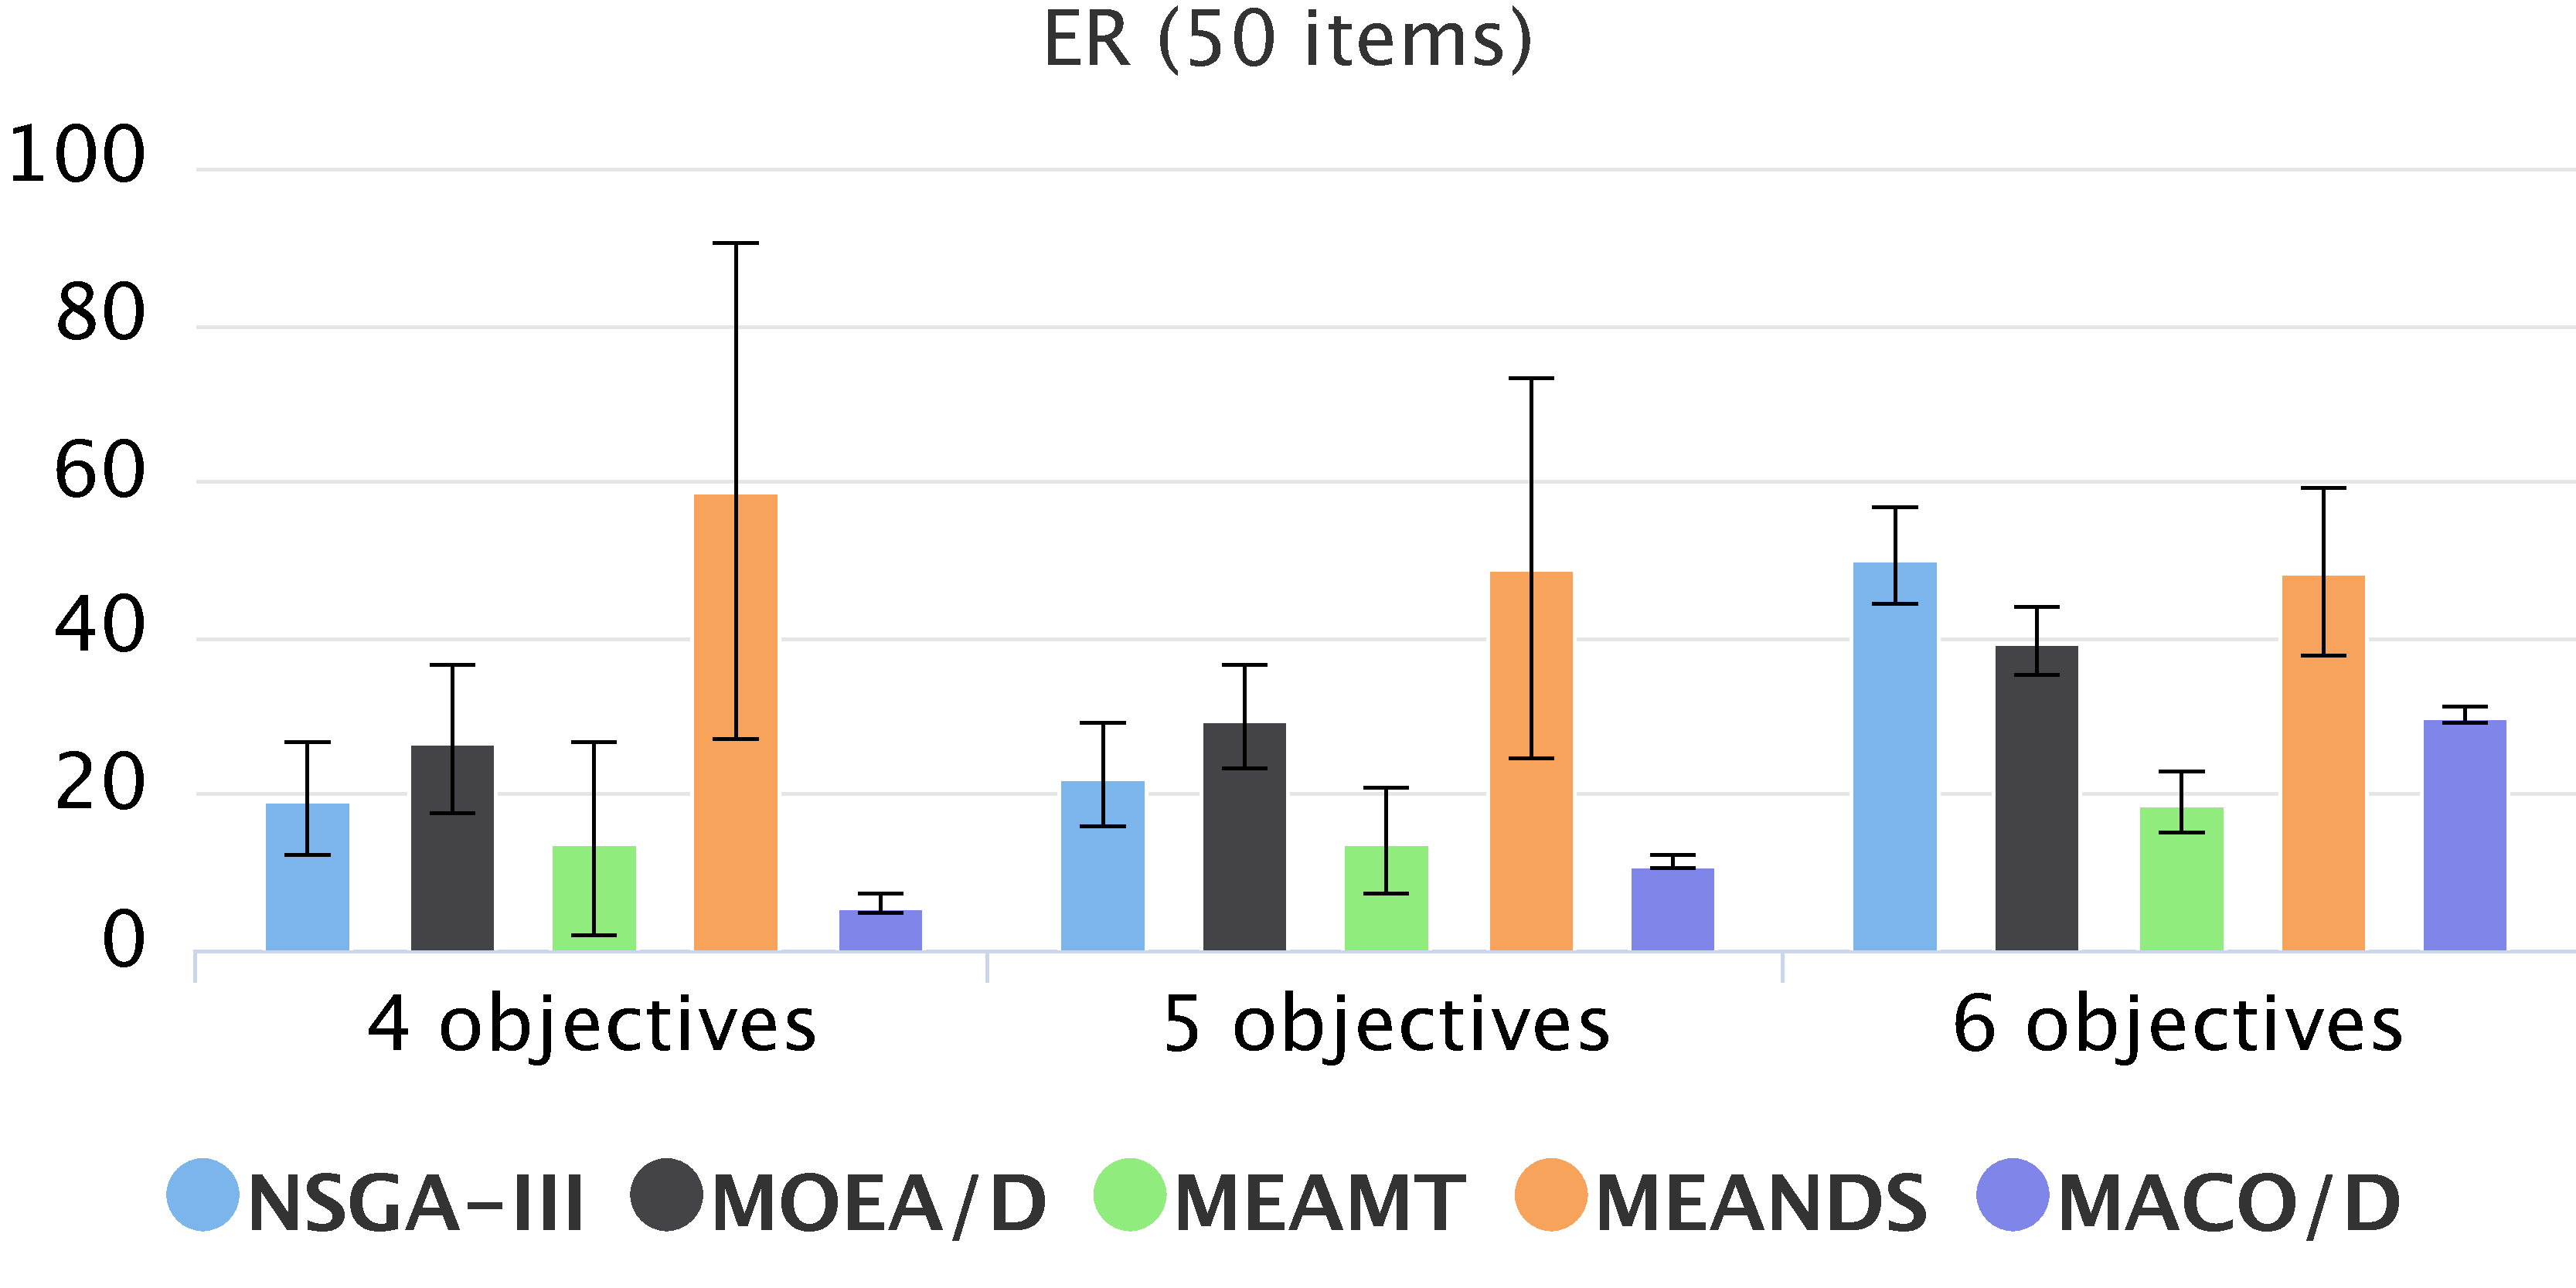
\includegraphics[width=0.5\textwidth]{cap_experimentos/figs/etapa3/er-mkp-50}
	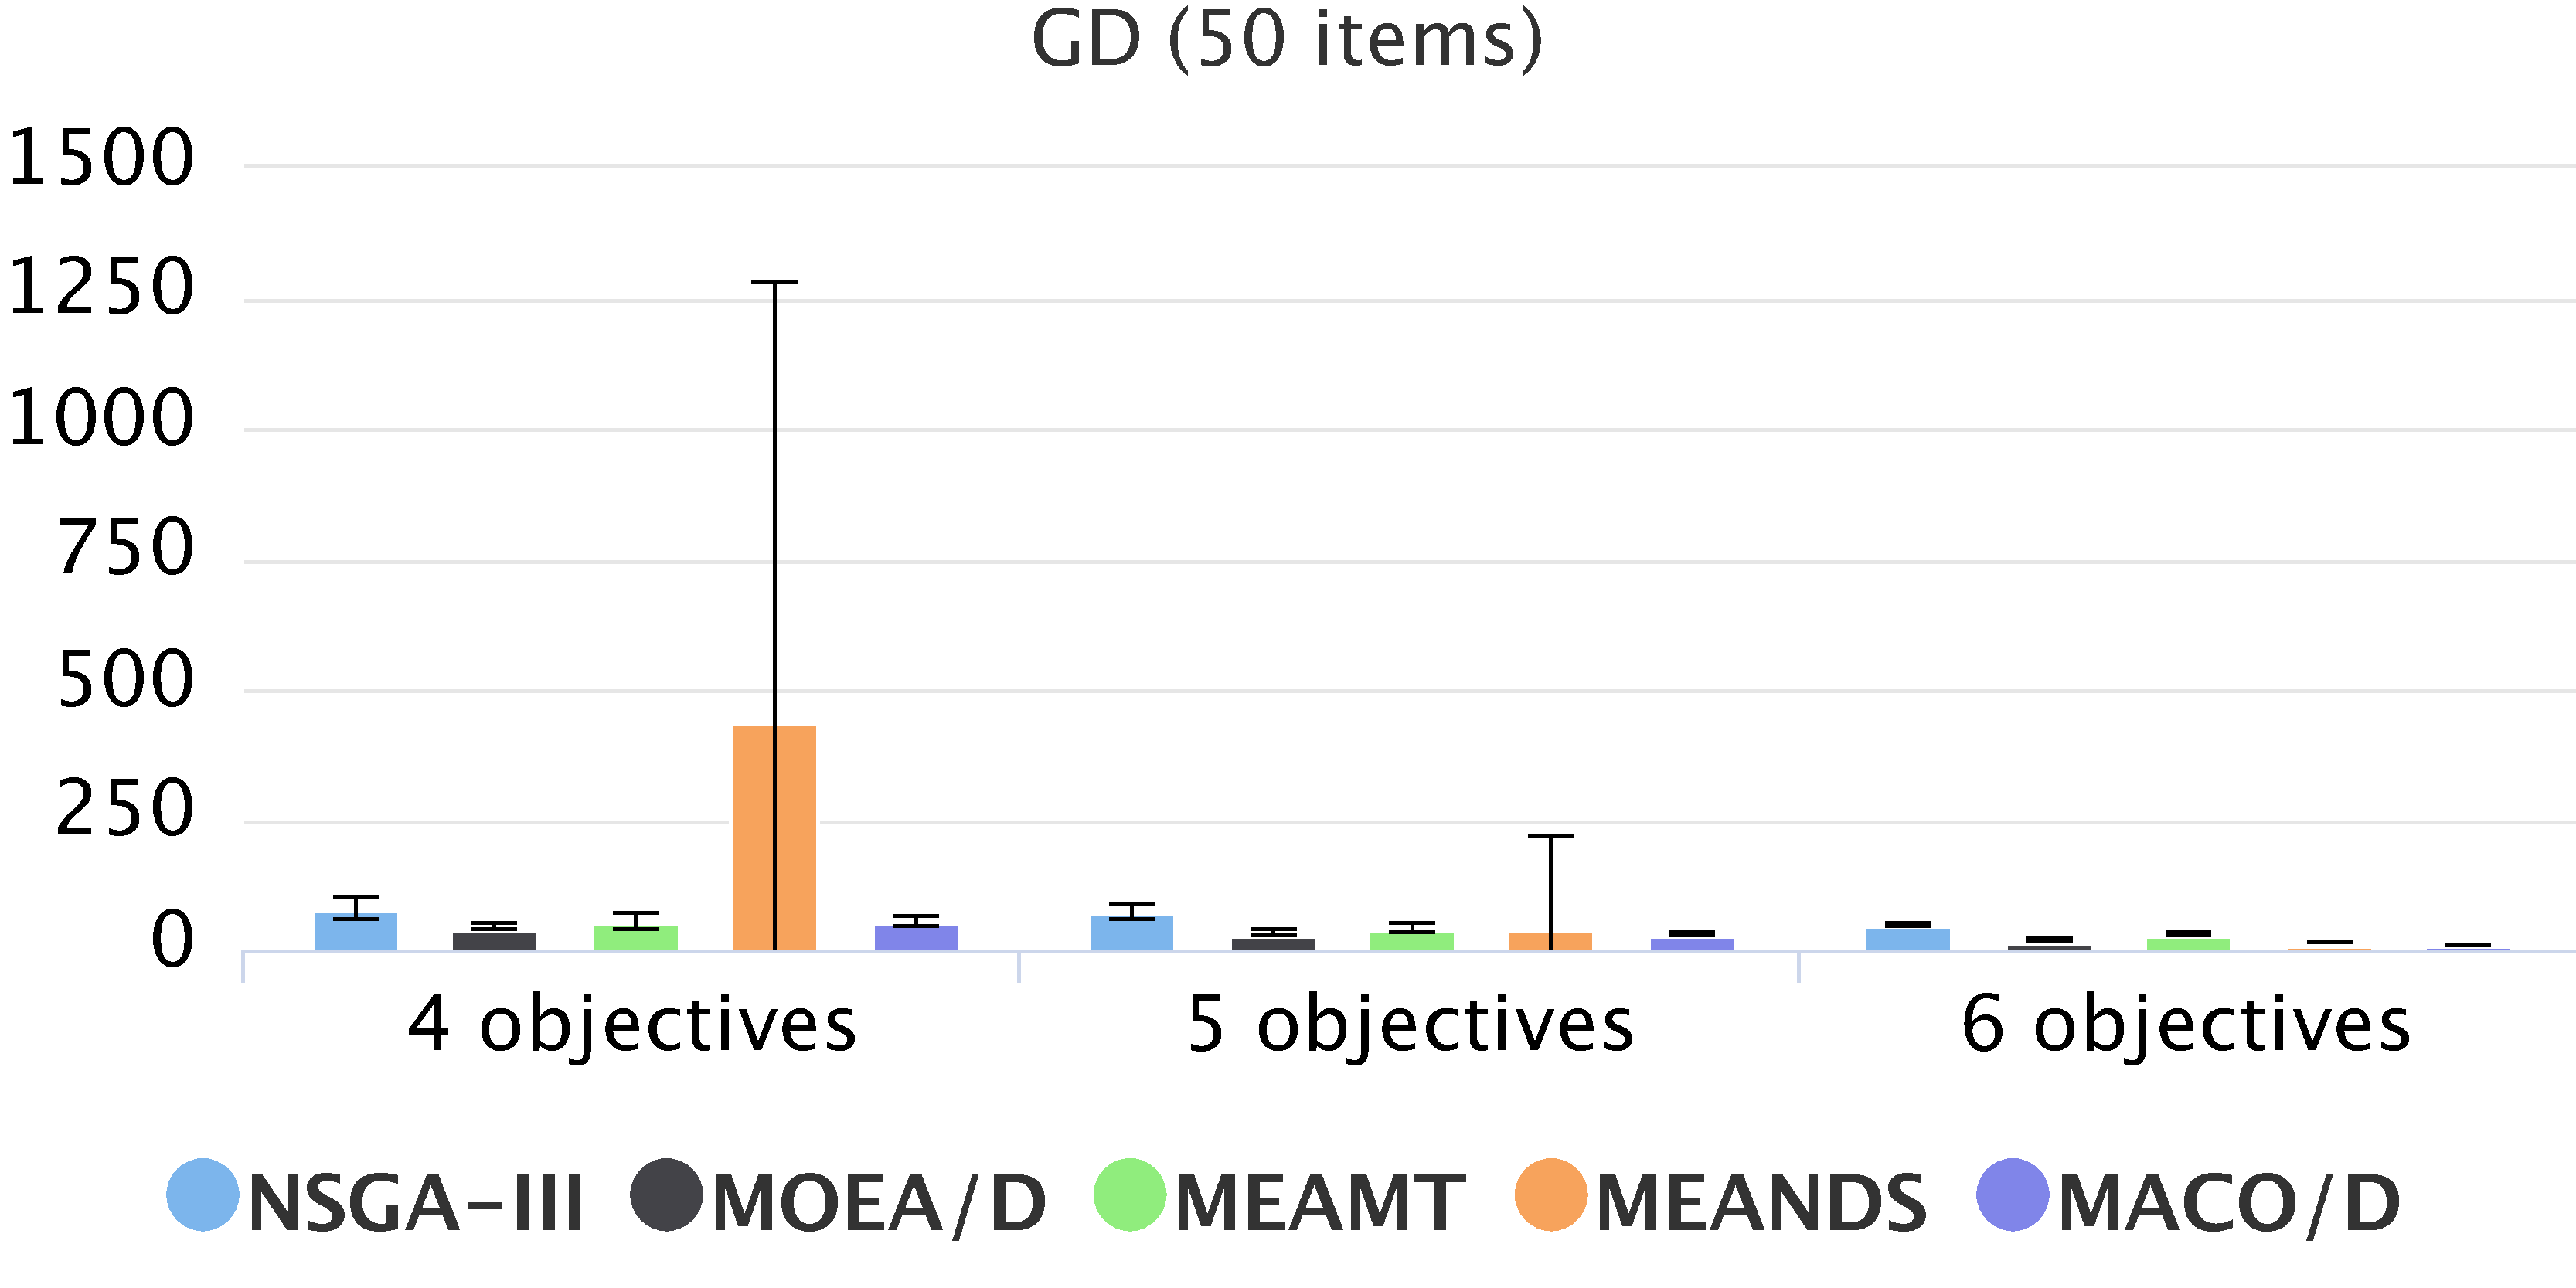
\includegraphics[width=0.5\textwidth]{cap_experimentos/figs/etapa3/gd-mkp-50}
	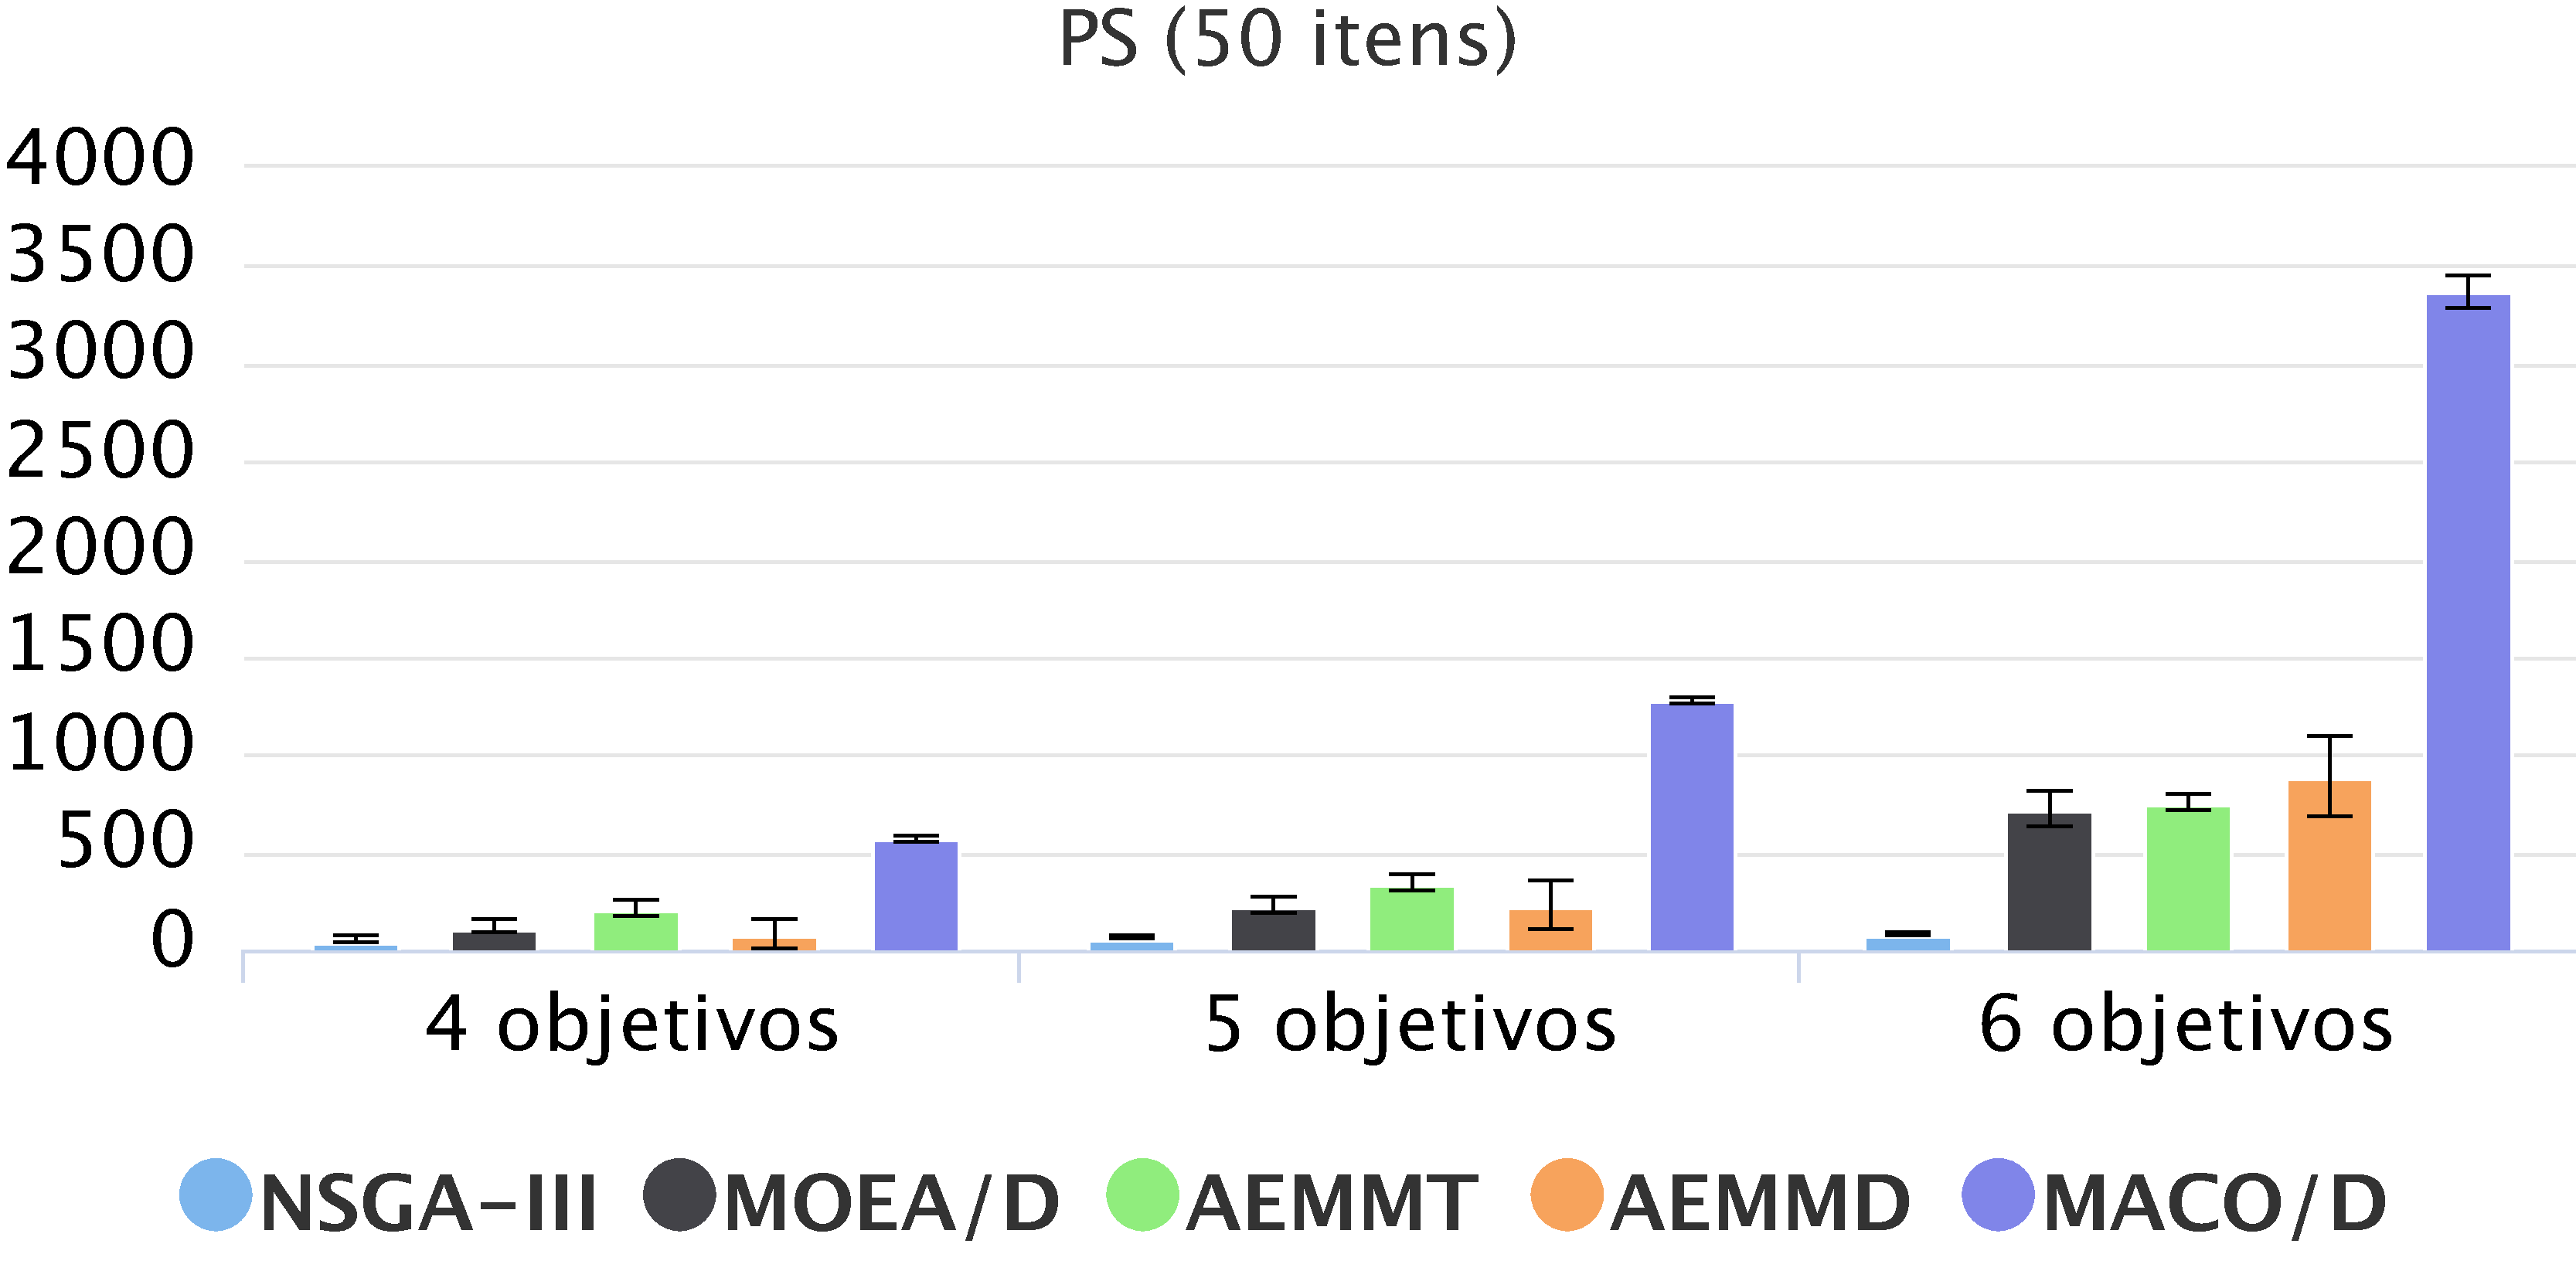
\includegraphics[width=0.5\textwidth]{cap_experimentos/figs/etapa3/ps-mkp-50}
	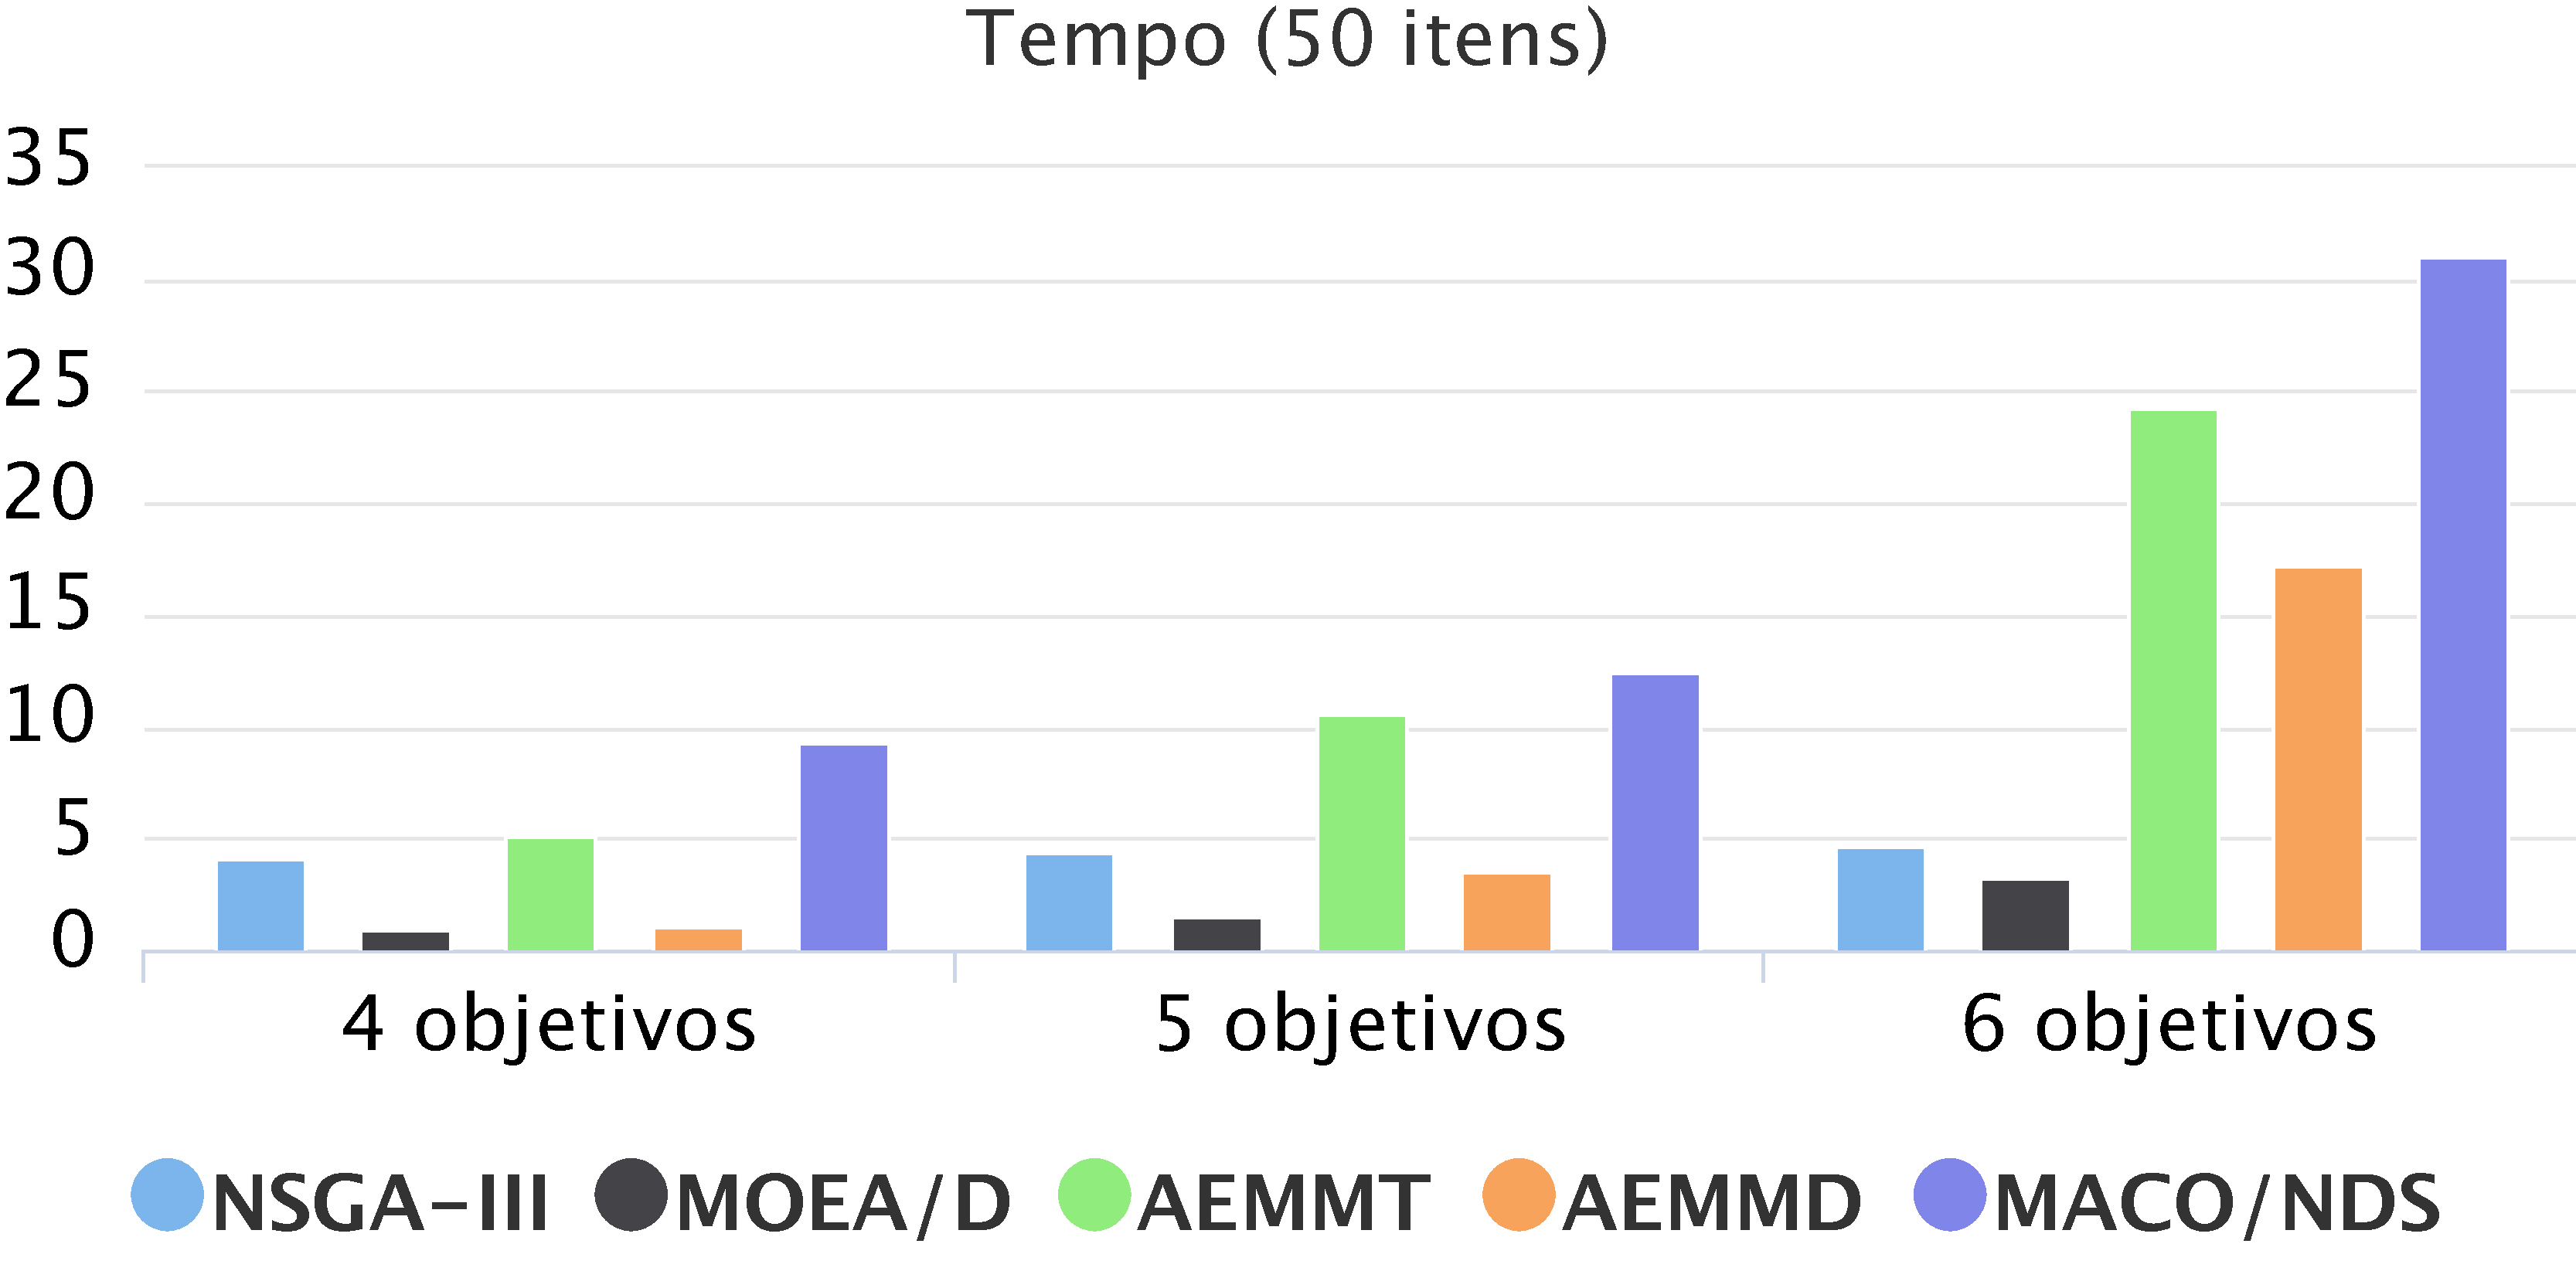
\includegraphics[width=0.5\textwidth]{cap_experimentos/figs/etapa3/time-mkp-50}
\end{figure*}

O PMM com 50 itens (figura \ref{fig_exp3_pmm_50}) apresenta comportamento similar às instâncias anteriores. O MACO/D e o AEMMT se revezam em menores taxas de erro, o MACO/D consegue menor $ER$ em 4 e 5 objetivos, enquanto o AEMMT apresenta melhor resultado em 6 objetivos. O MACO/D obtém os melhores valores de $GD$ e $PS$, e o MOEA/D é o algoritmo mais rápido.

\begin{figure*}[!htbp]
	\caption{Etapa 3: resultados agrupados para o PMM com 30, 40 e 50 itens}
	\label{fig_exp3_pmm_todos}
	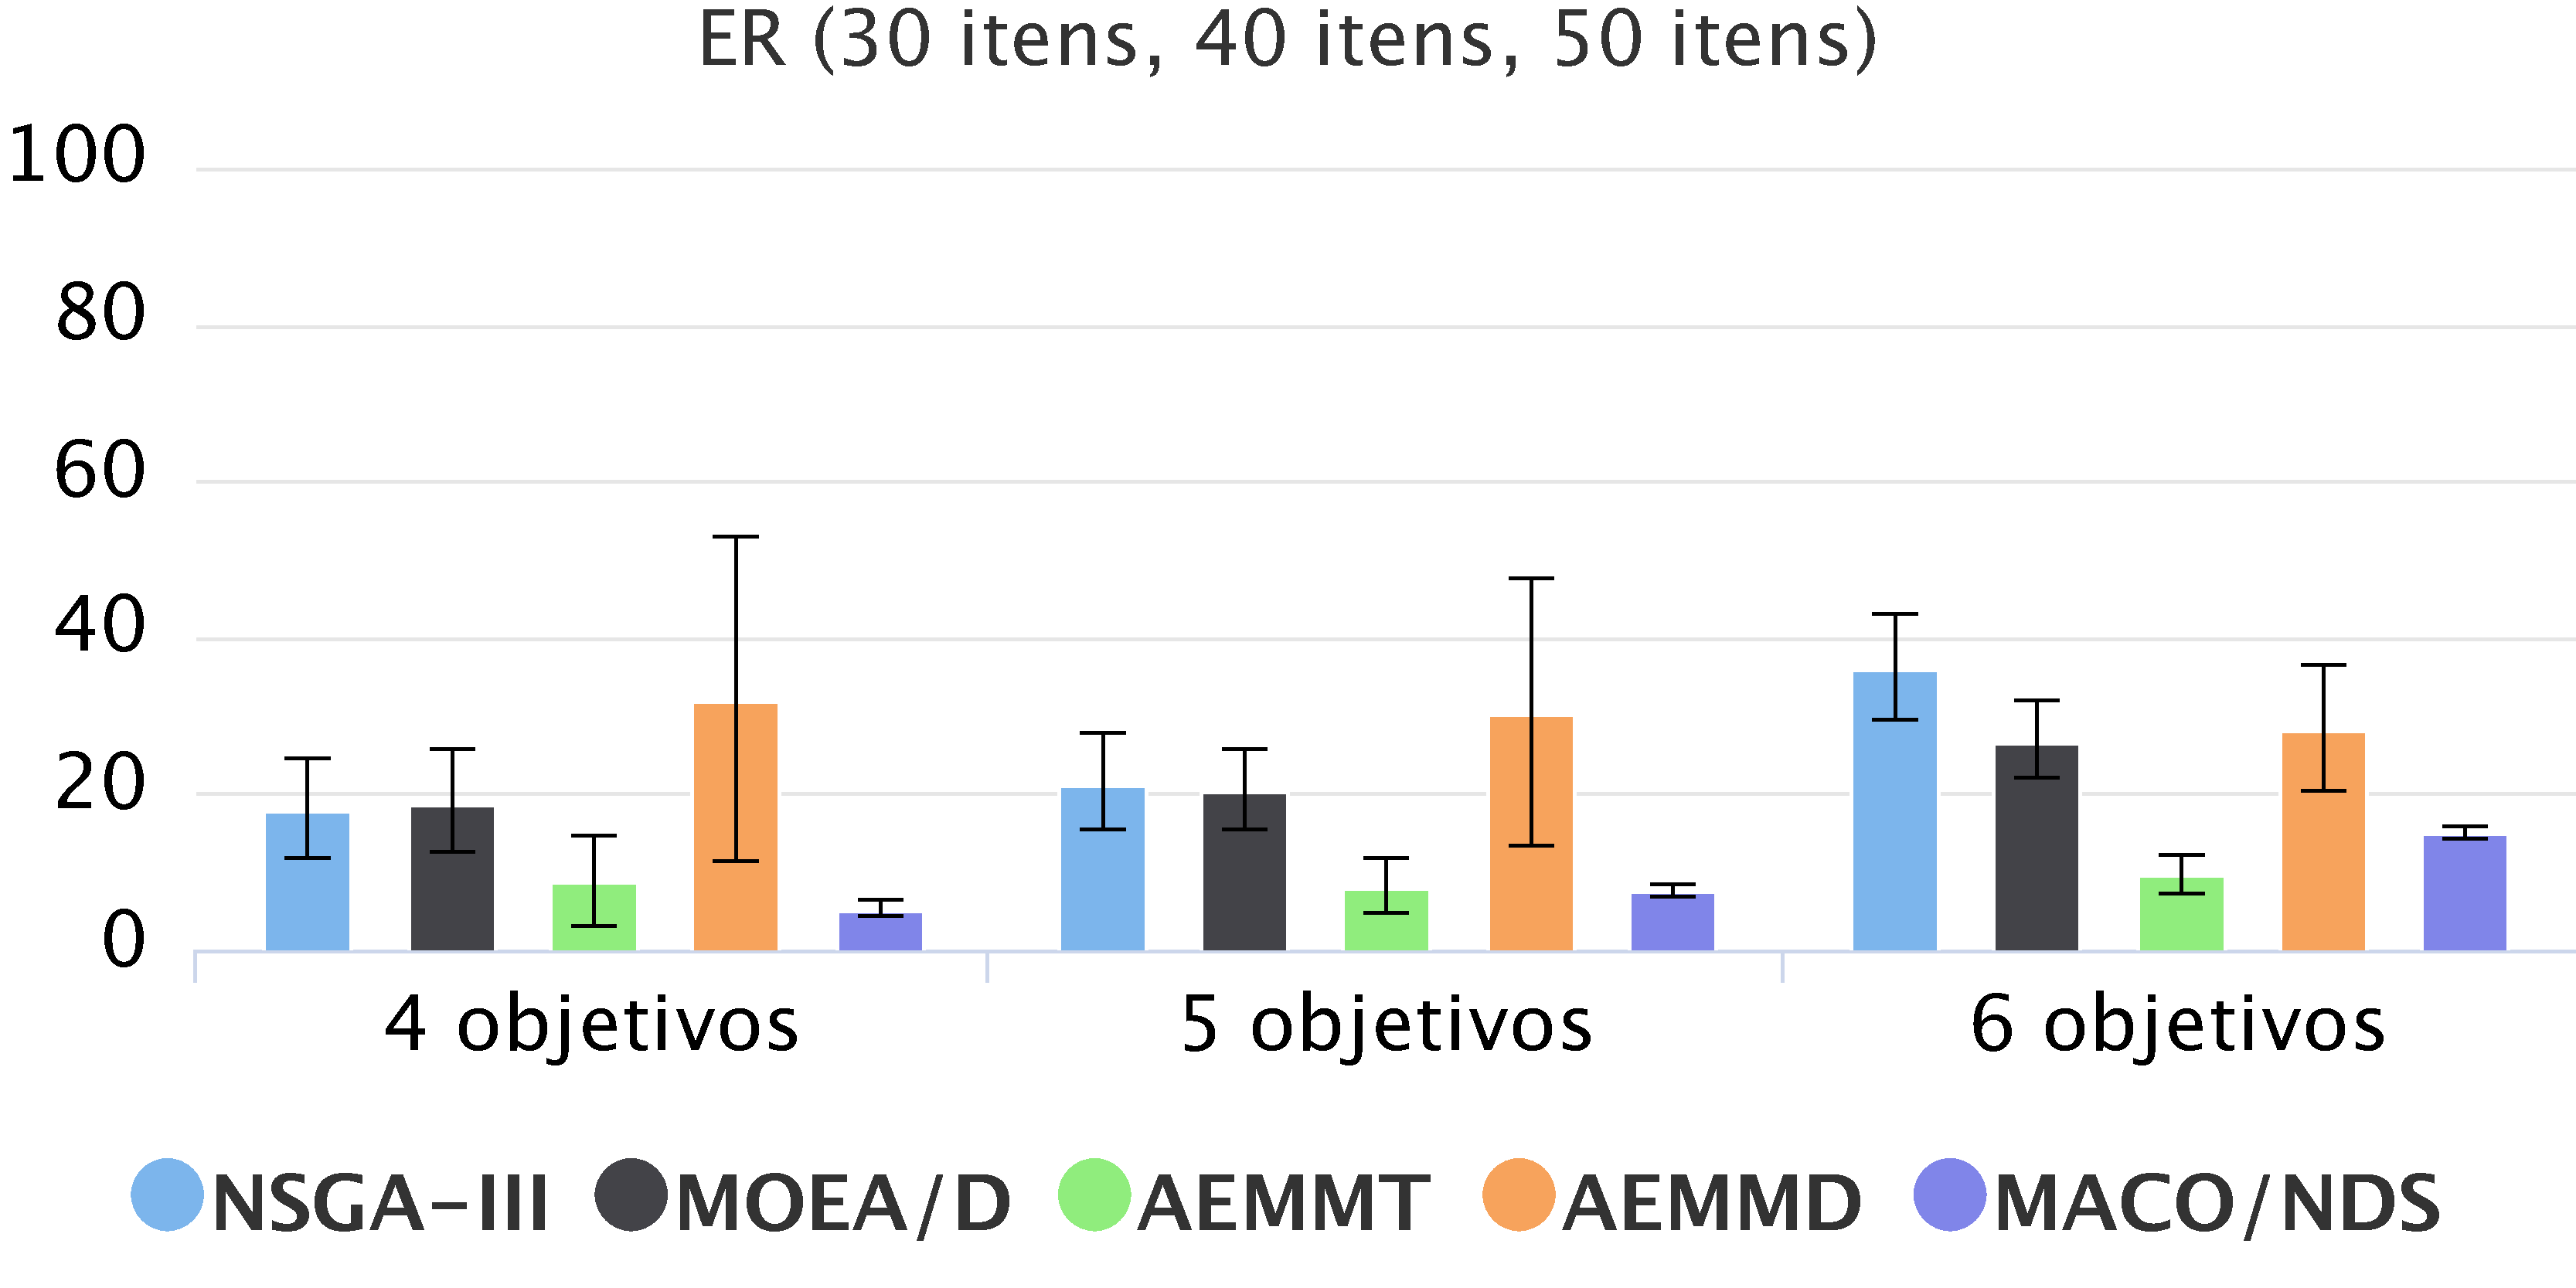
\includegraphics[width=0.5\textwidth]{cap_experimentos/figs/etapa3/er-mkp-todos}
	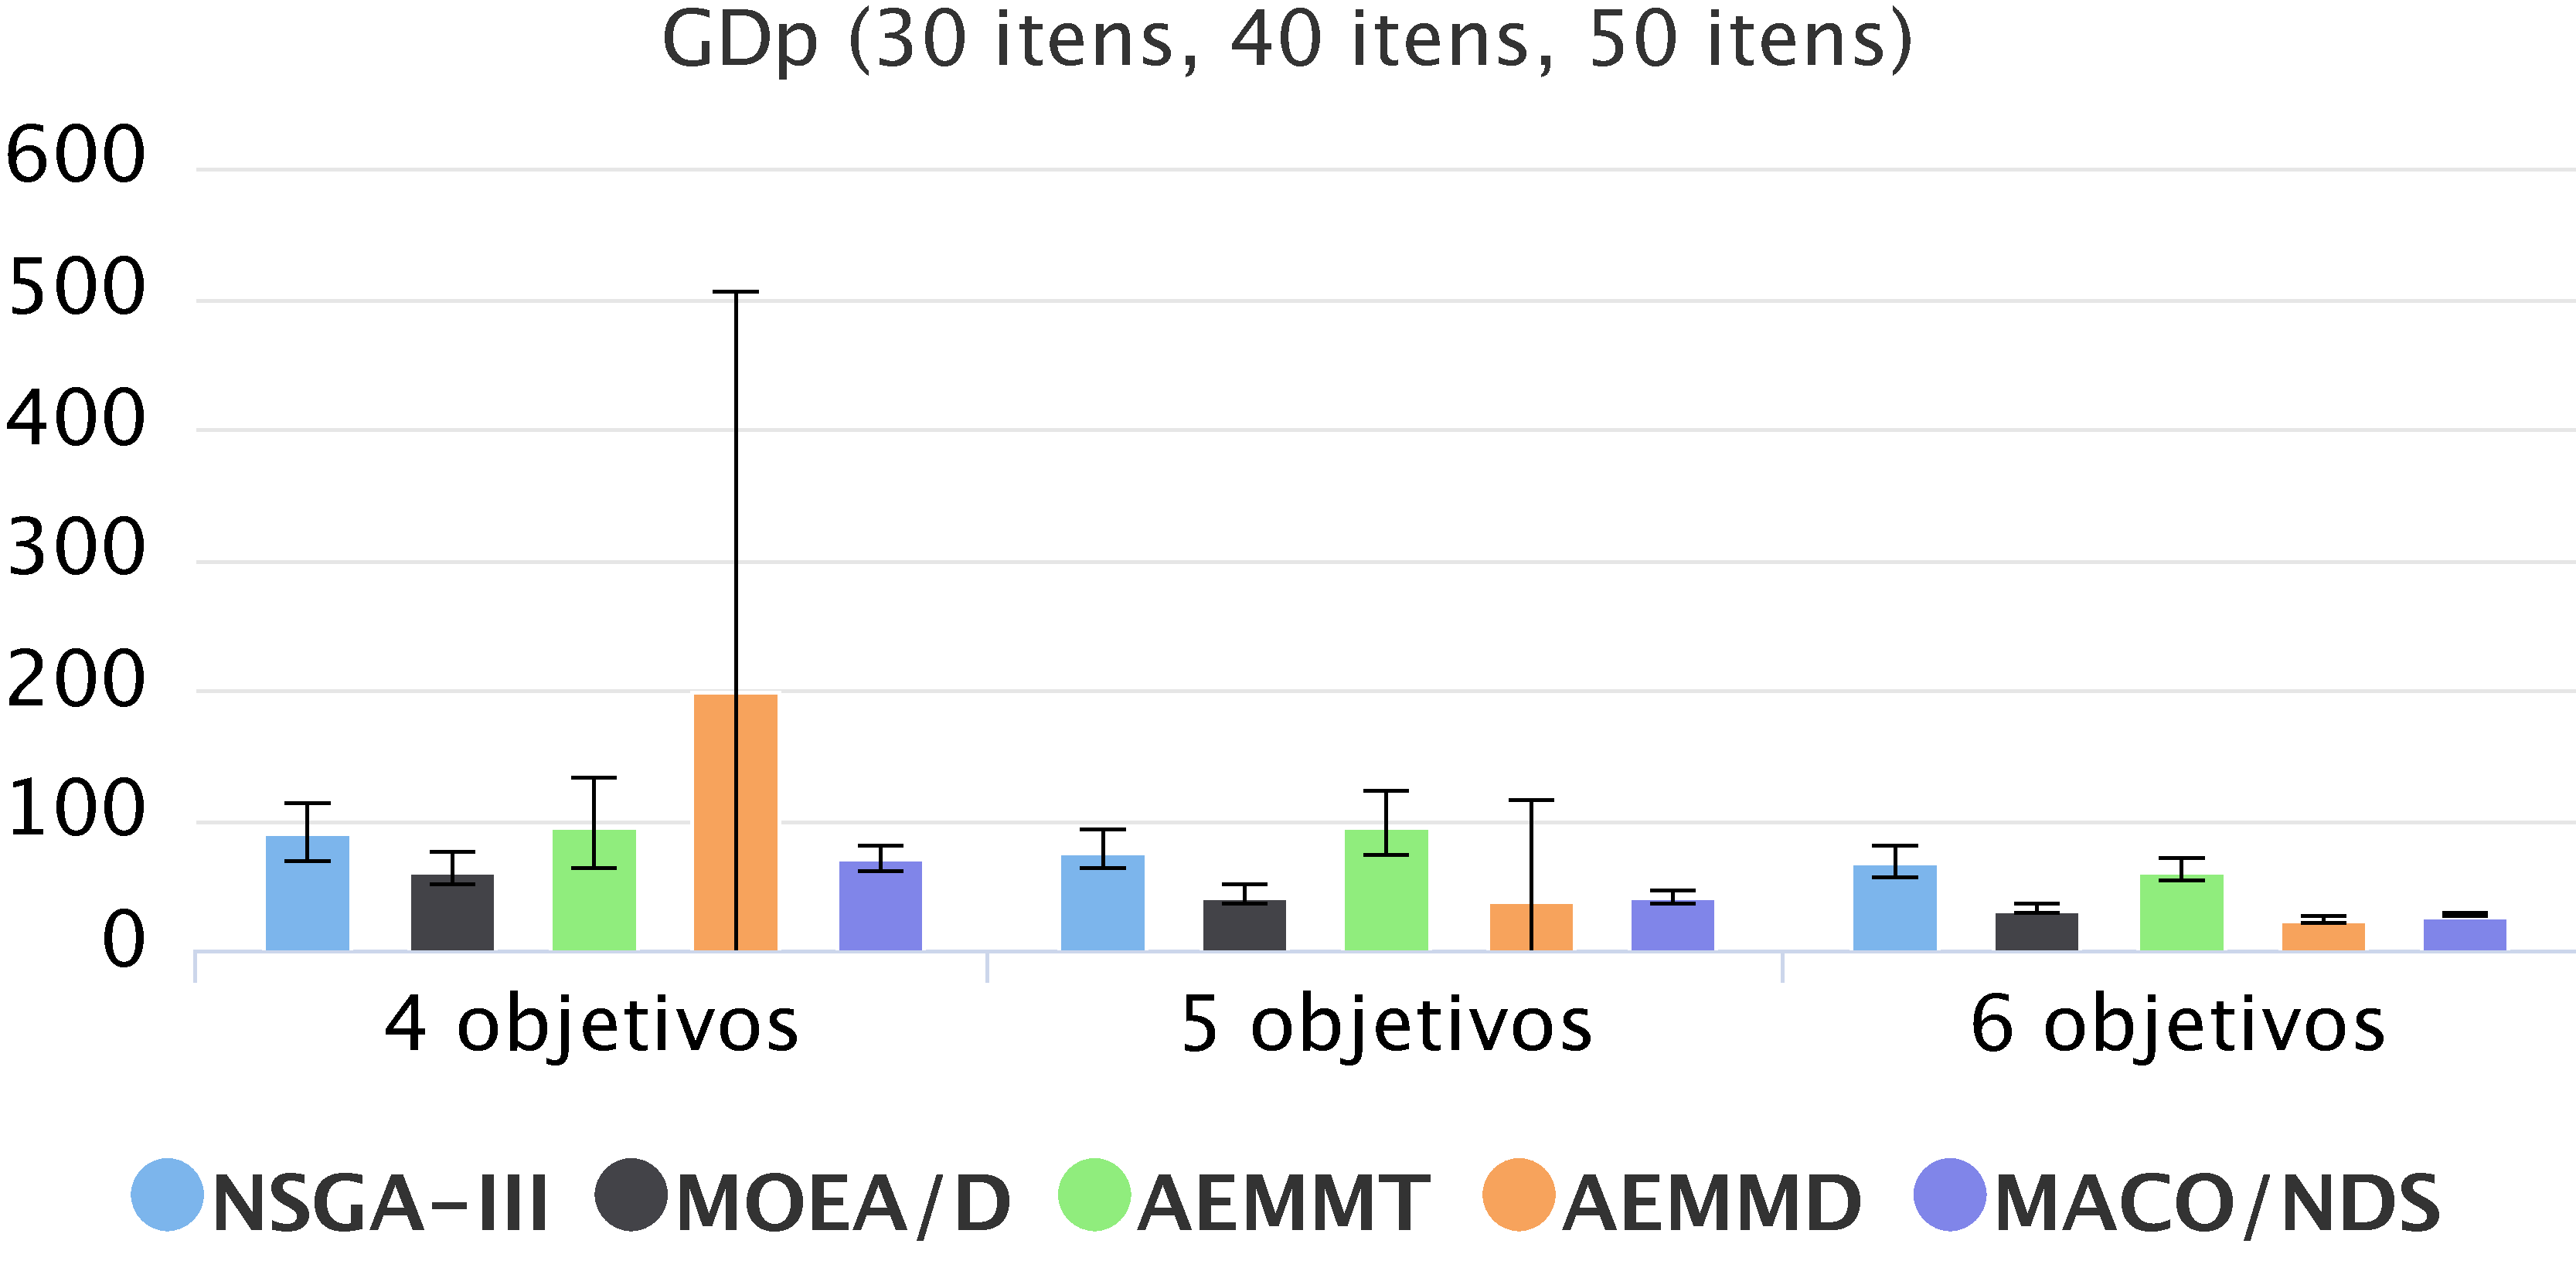
\includegraphics[width=0.5\textwidth]{cap_experimentos/figs/etapa3/gd-mkp-todos}
	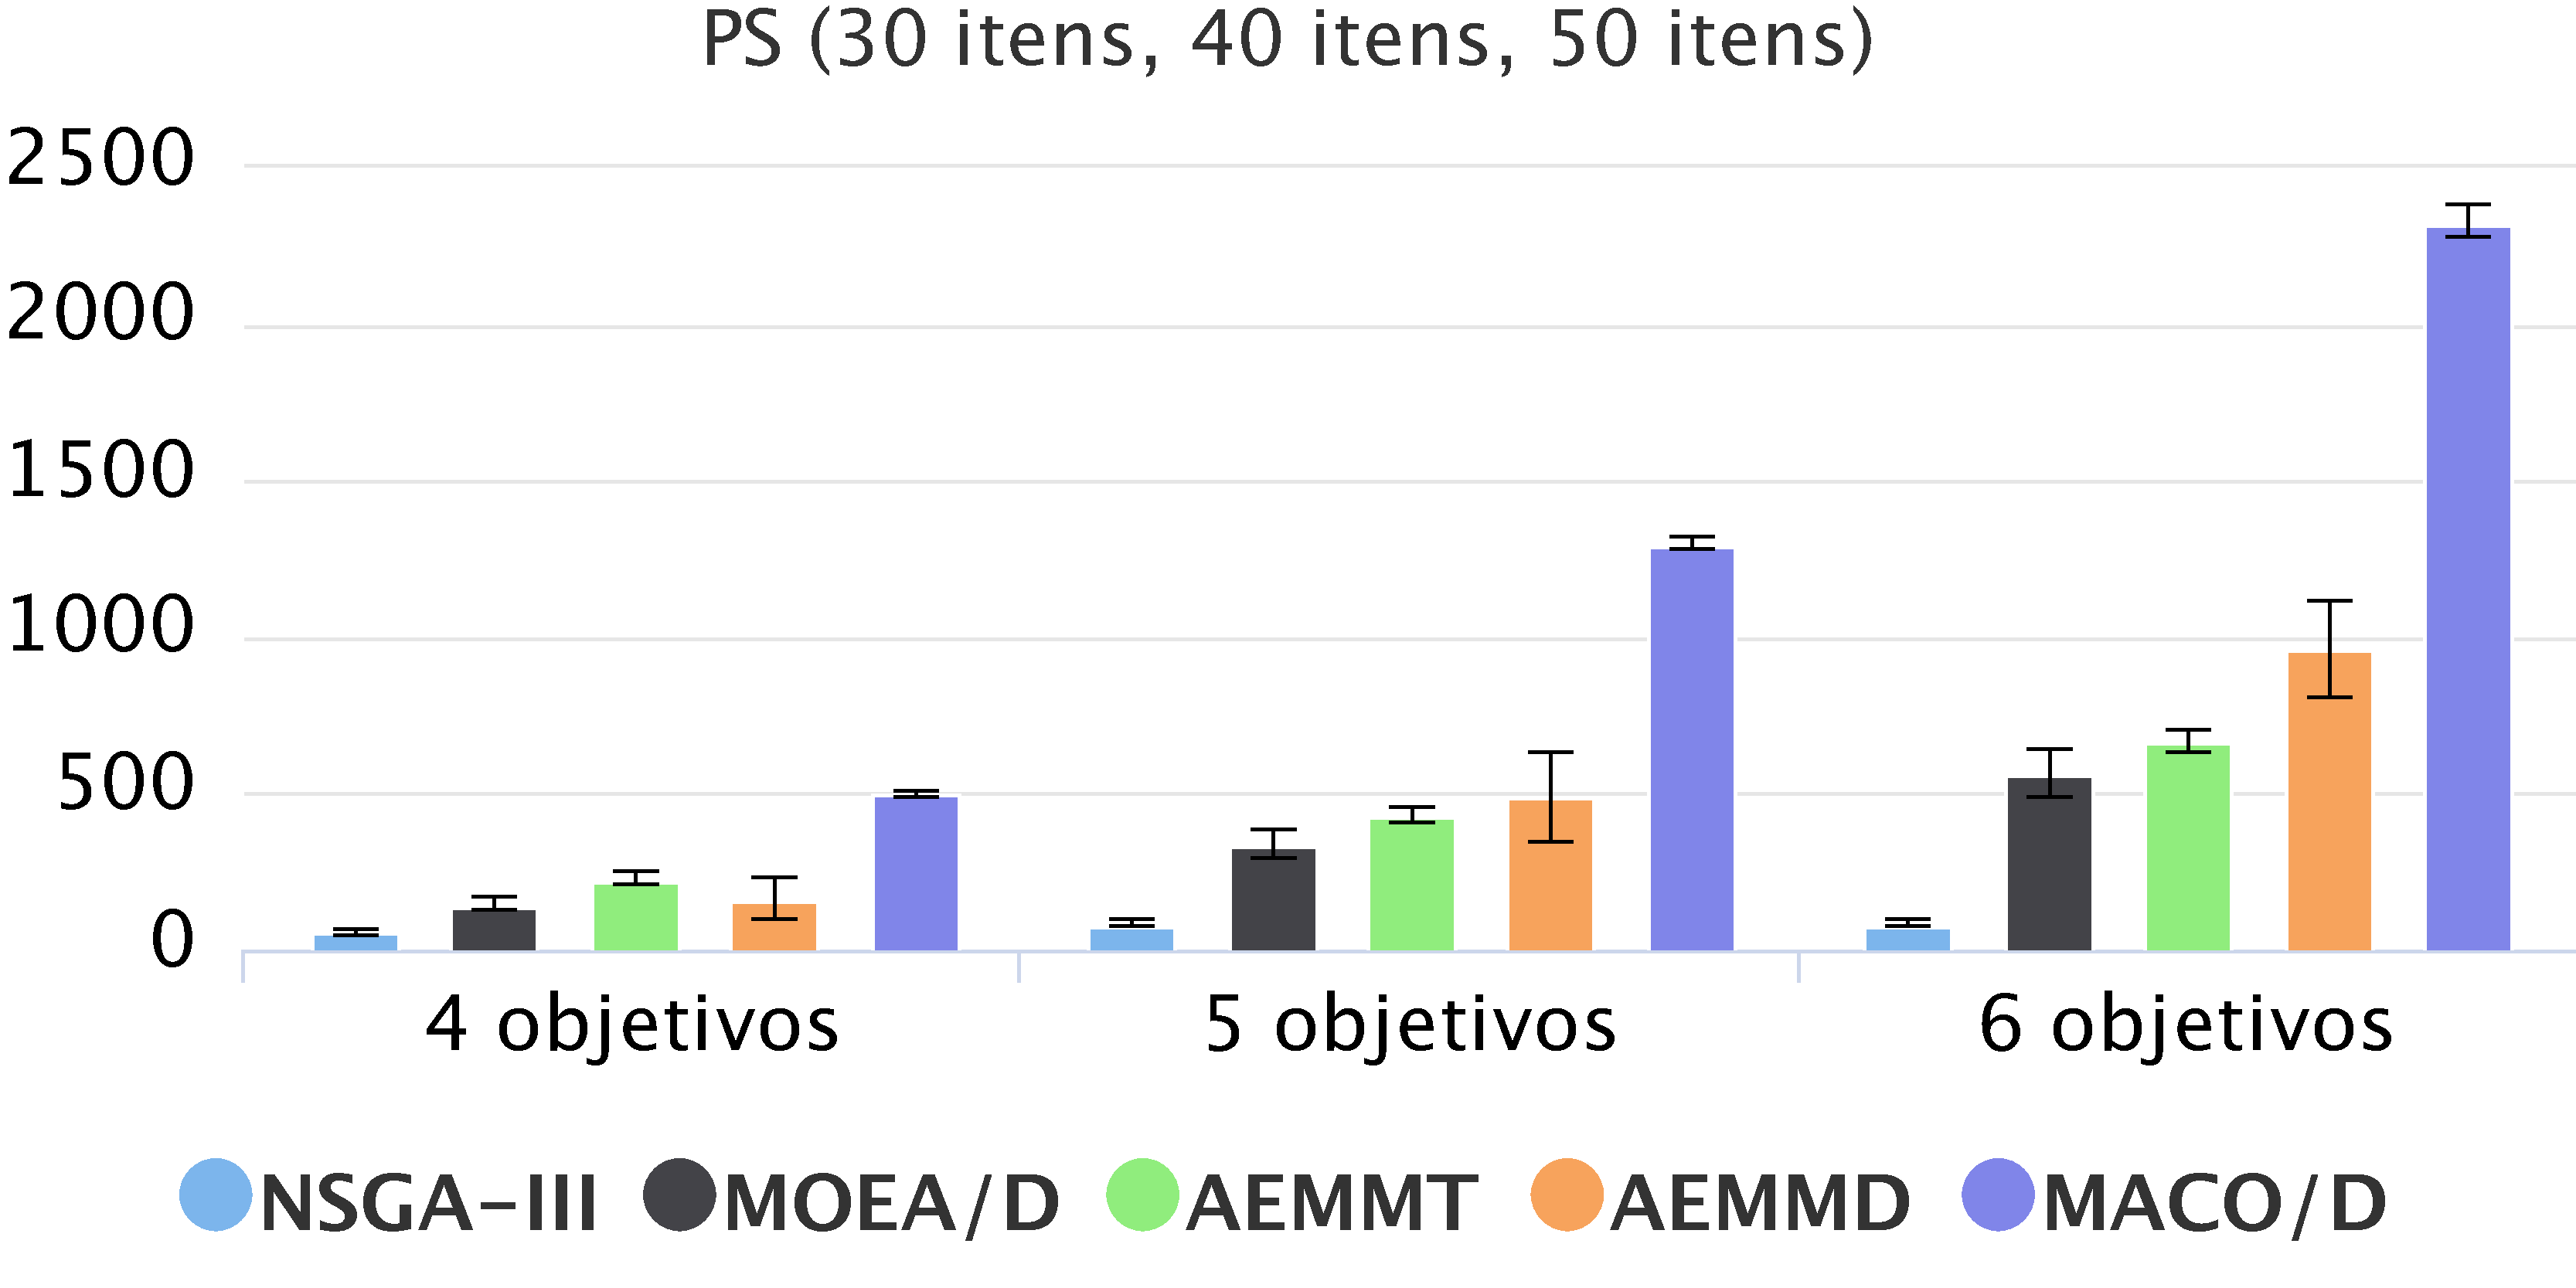
\includegraphics[width=0.5\textwidth]{cap_experimentos/figs/etapa3/ps-mkp-todos}
	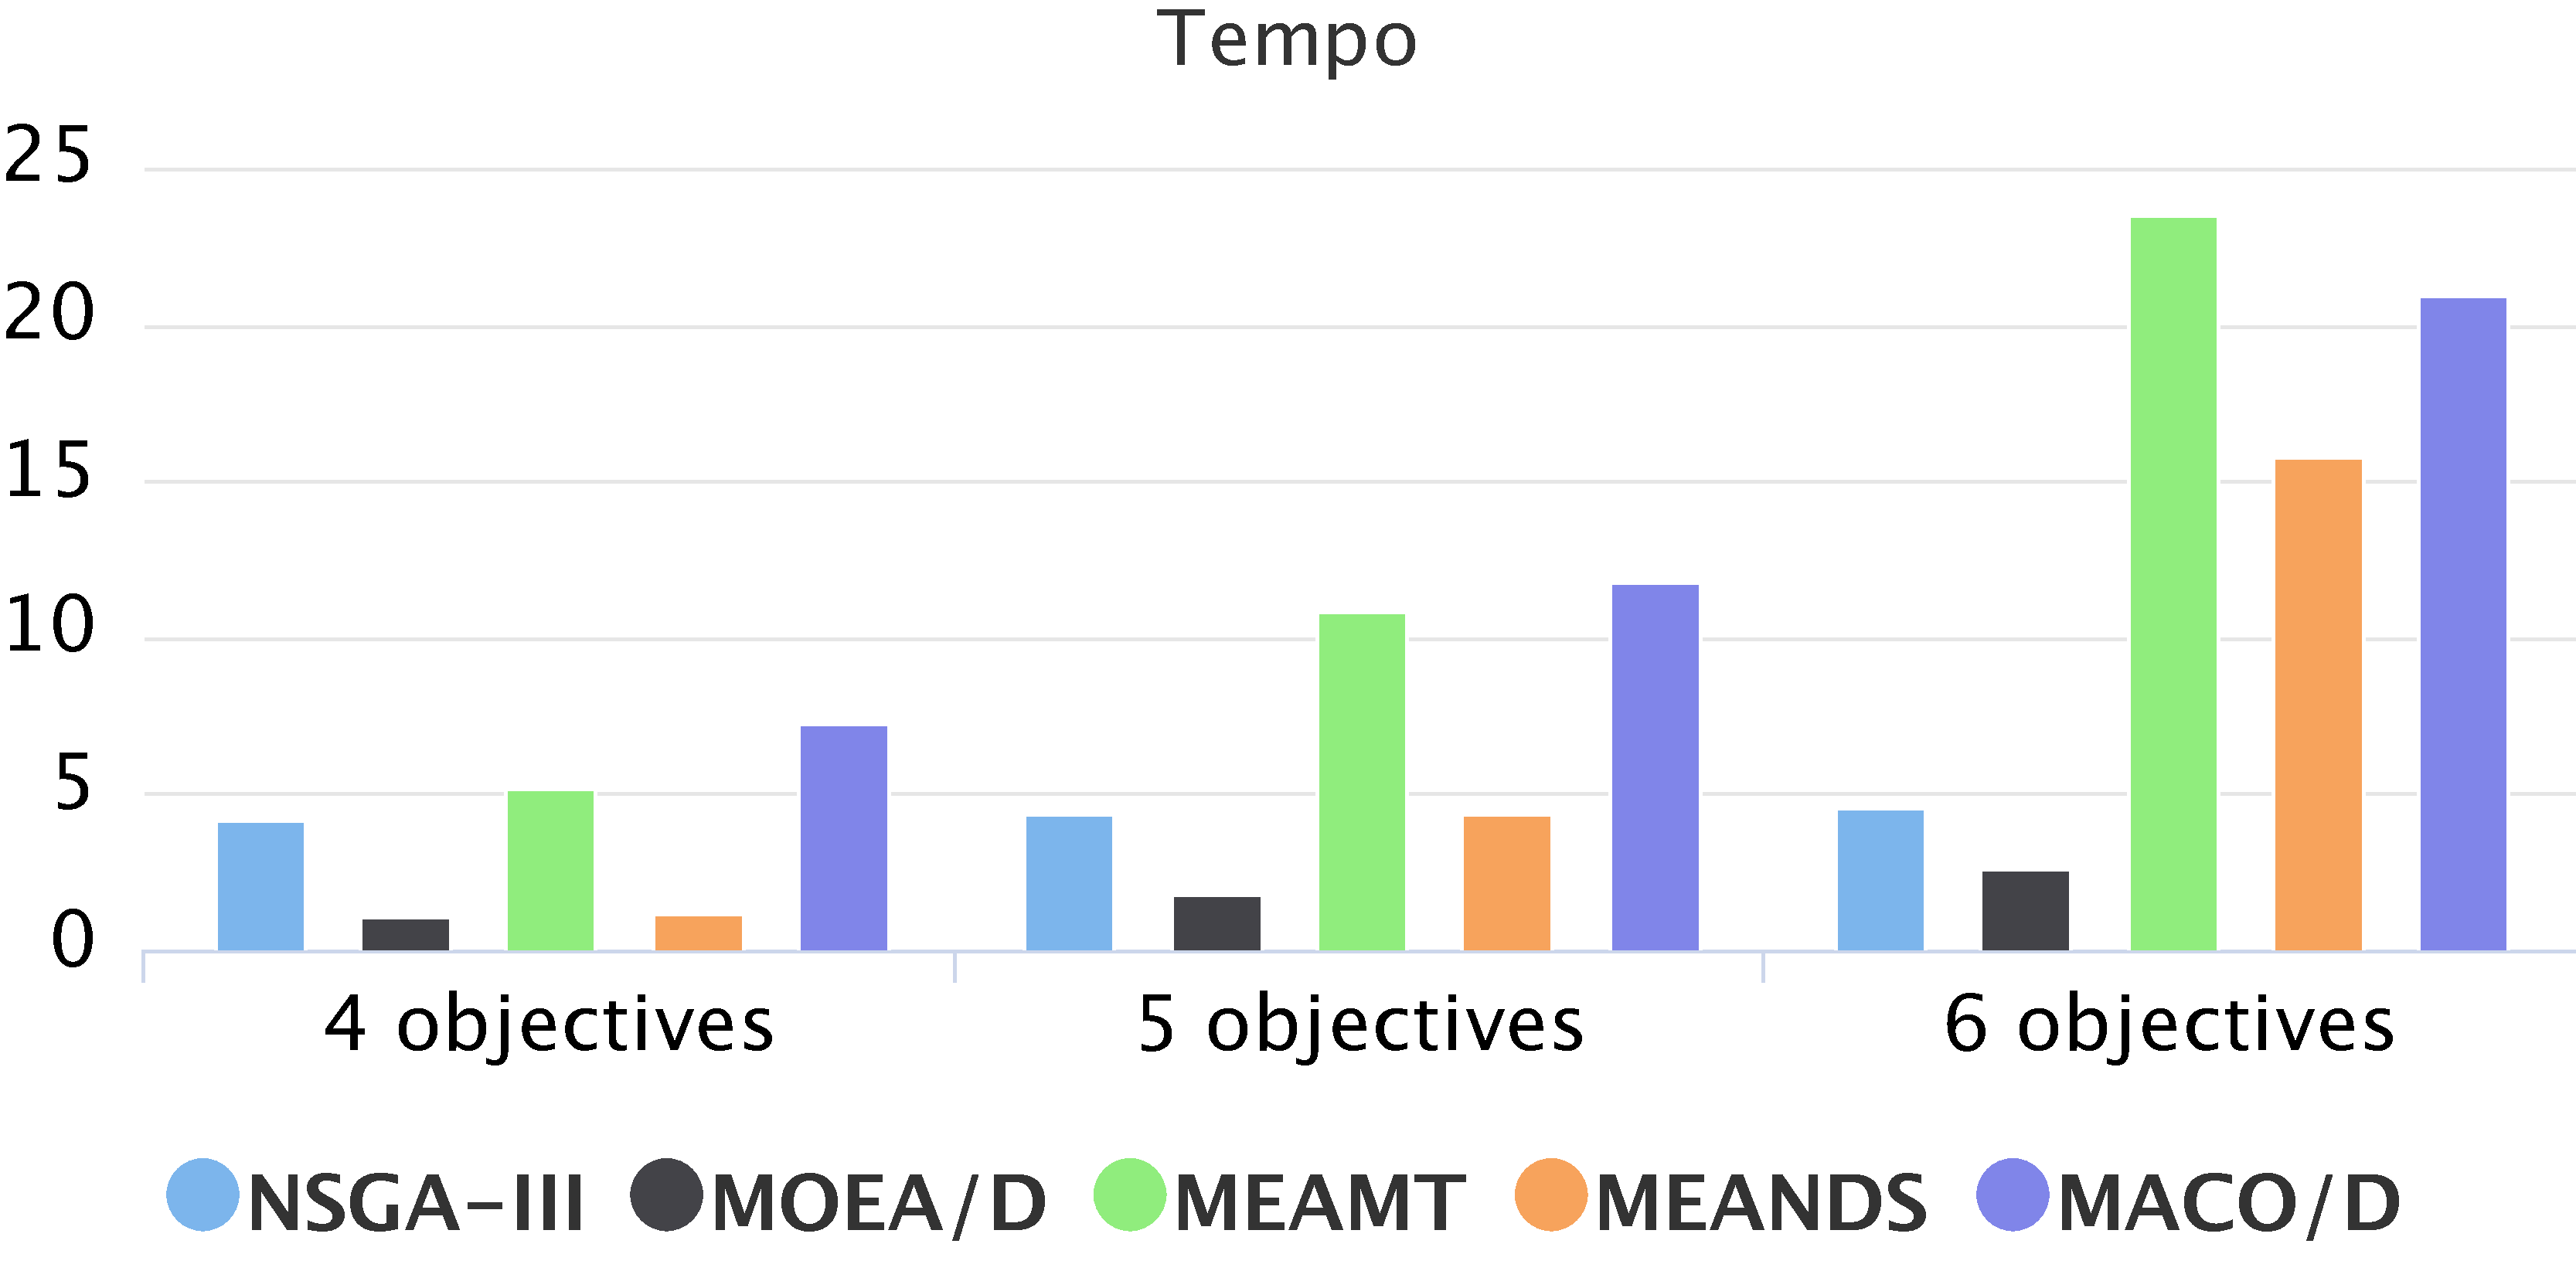
\includegraphics[width=0.5\textwidth]{cap_experimentos/figs/etapa3/time-mkp-todos}
\end{figure*}

A fim de se fazer uma análise conjunta dos resultados, a média entre os 3 cenários é apresentada nos gráficos da figura \ref{fig_exp3_pmm_todos}. As taxas de erro são muito baixas para ambos AEMMT e MACO/D quando comparados aos demais algoritmos. Os resultados em $GD$ são bons para a maioria dos métodos, apenas o AEMMD apresenta um valor ruim de GD no problema de 4 objetivos. O MOEA/D produz o melhor $GD$ no problema de 4 objetivos, enquanto que em 5 e 6 objetivos, o MACO/D e o AEMMD consegue valores bem similares. É importante notar que os desvio padrões no AEMMD são altos, o que pode representar uma certa inconsistência do método em gerar boas soluções. O $PS$ é , de longe, dominado pelo MACO/D. Em questão de tempo de execução, o AEMMT, o AEMMD e o MACO/S variam bastante com o número de objetivos, enquanto os demais são estáveis. O MOEA/D é o algoritmo mais rápido entre os avaliados nesta etapa dos experimentos. O NSGA-III não é pior método em nenhuma das formulações de objetivo, mas também não se destaca em nenhum dos critérios de avaliação.

\begin{figure*}[!htbp]
	\caption{Etapa 3: resultados para o PRM na rede $R_1$}
	\label{fig_exp3_prm_r1}
	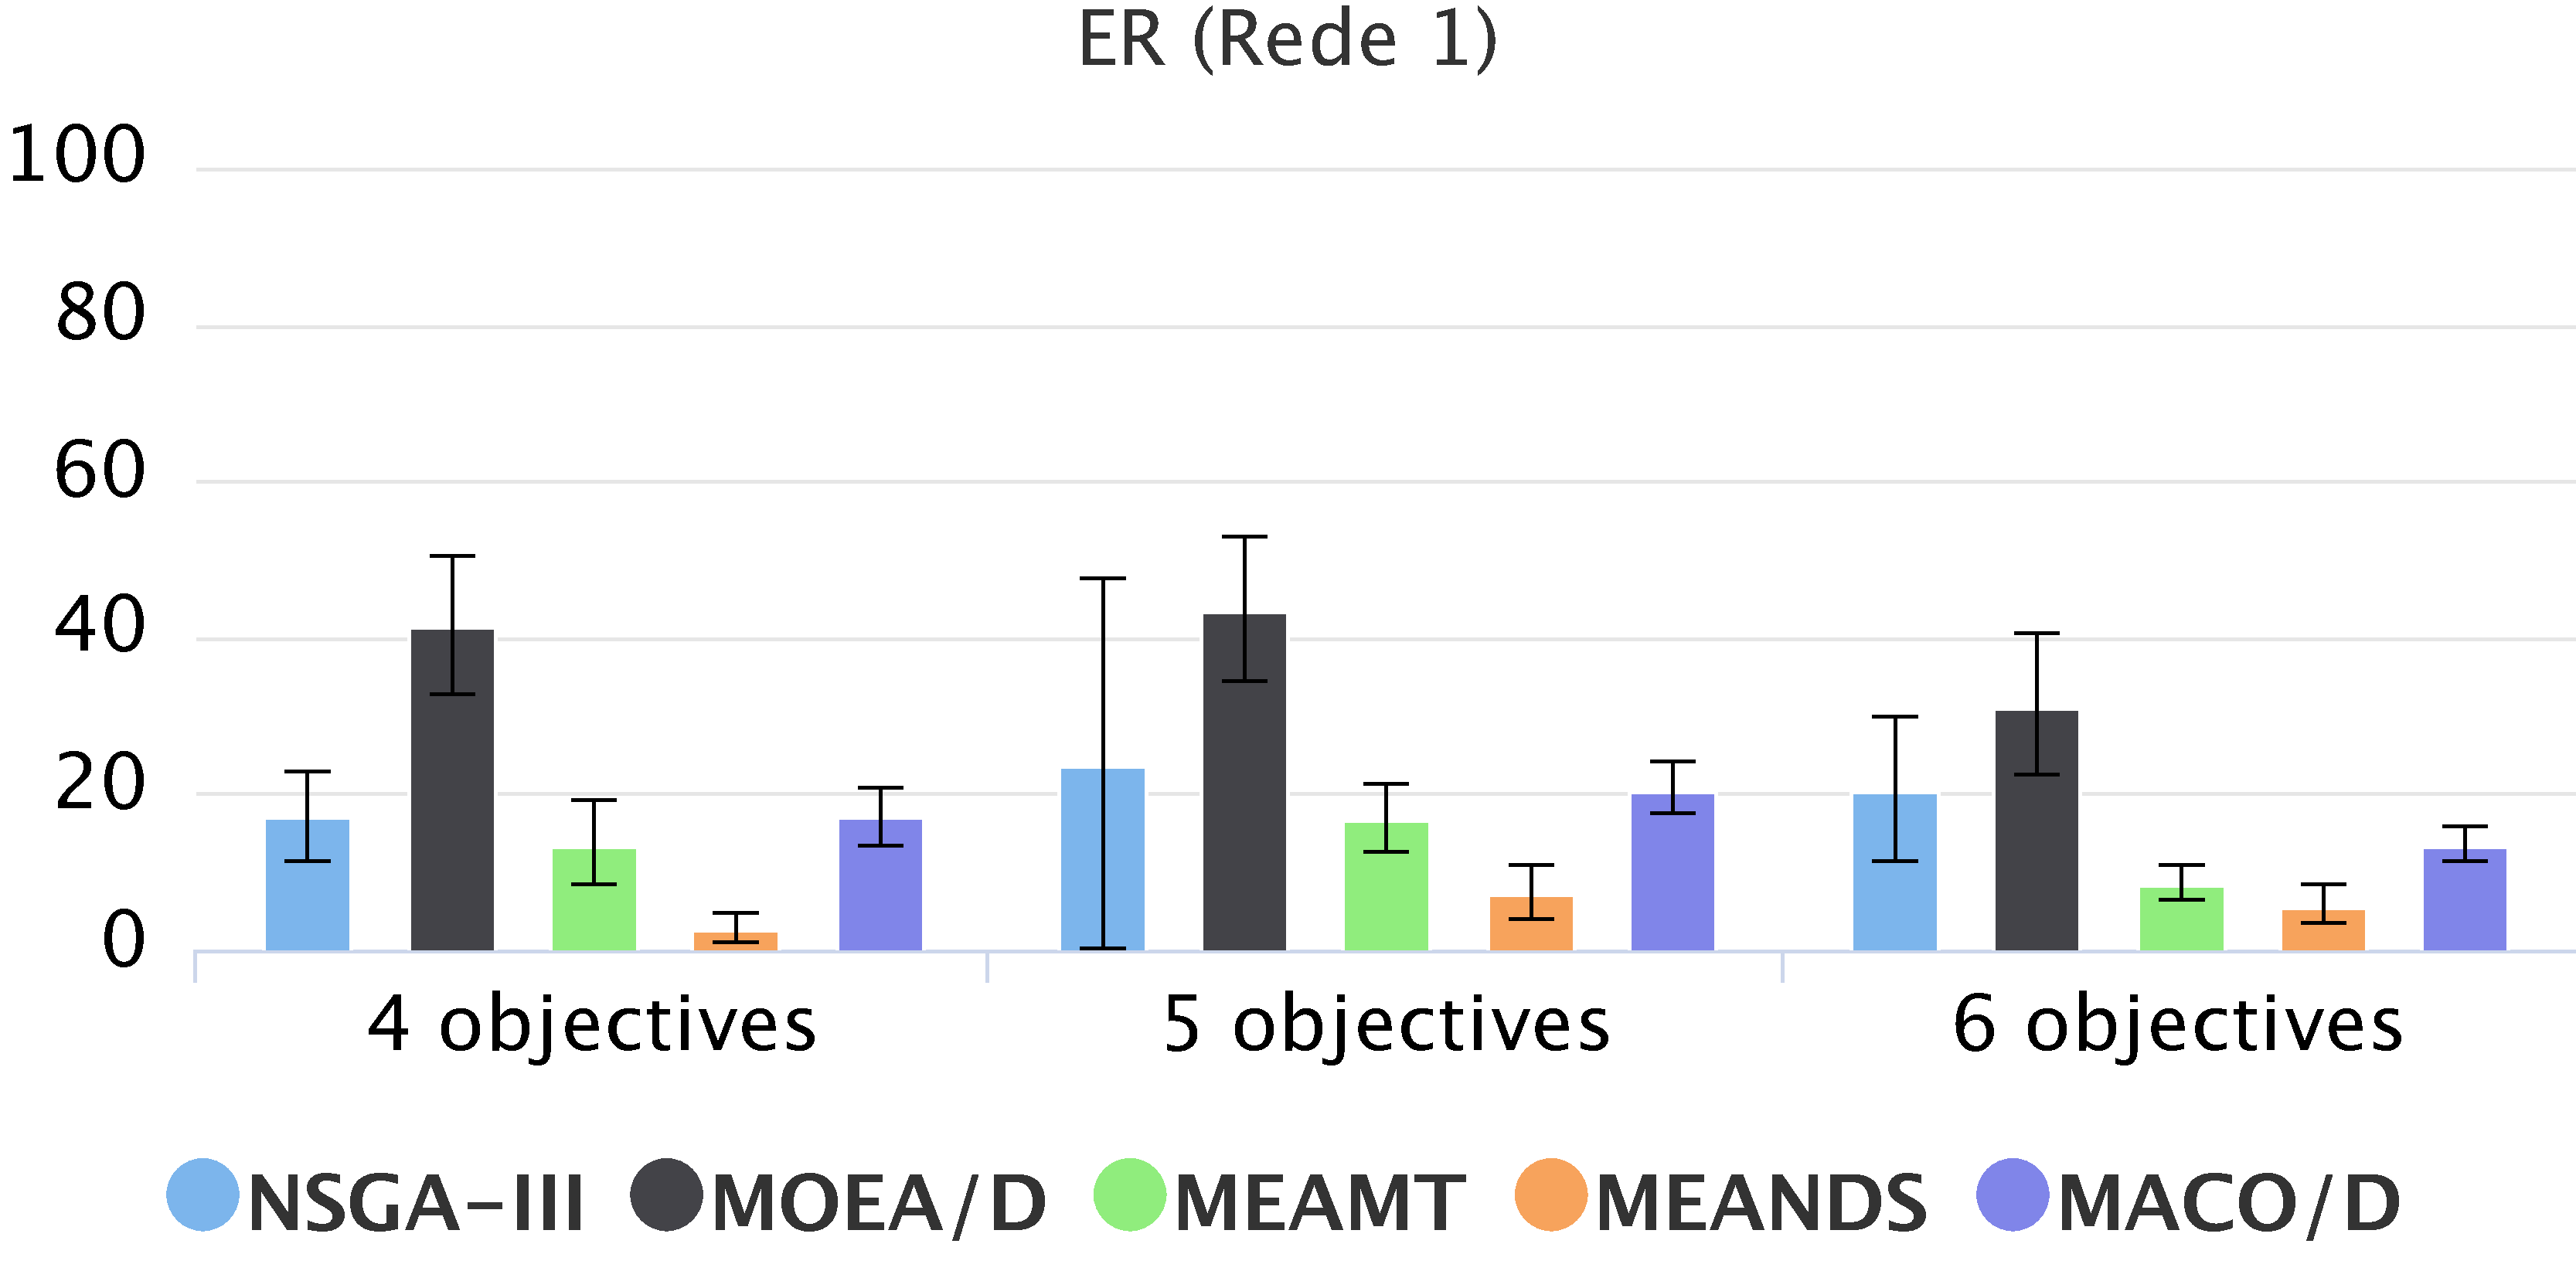
\includegraphics[width=0.5\textwidth]{cap_experimentos/figs/etapa3/er-mrp-r1}
	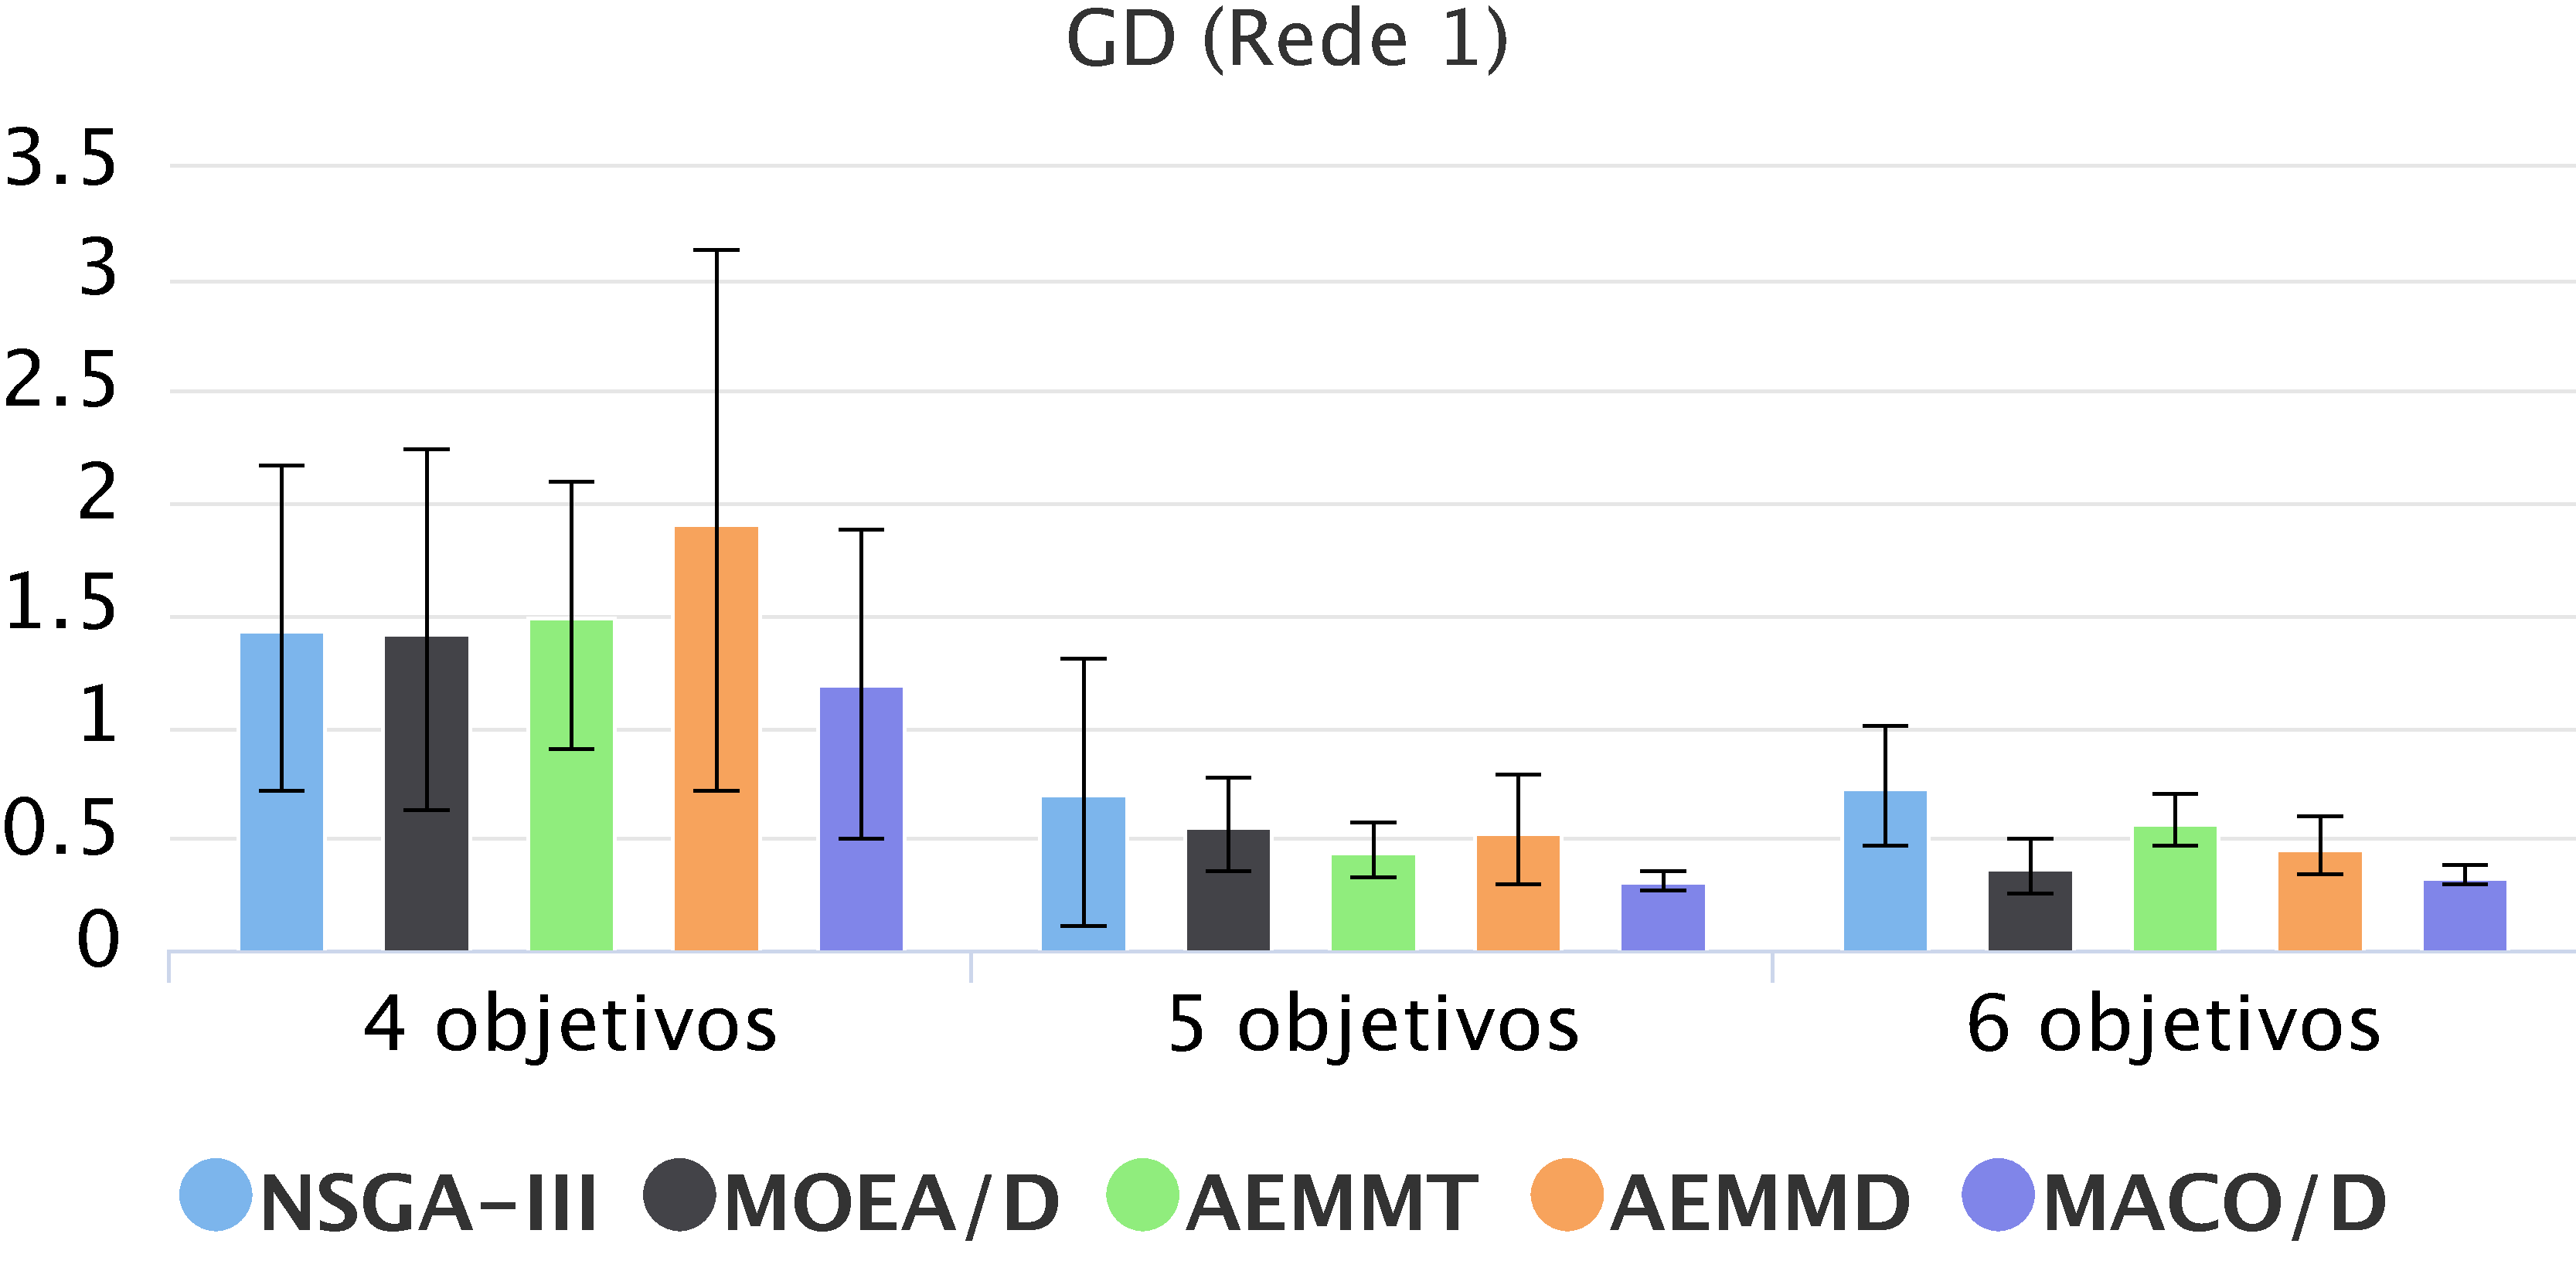
\includegraphics[width=0.5\textwidth]{cap_experimentos/figs/etapa3/gd-mrp-r1}
	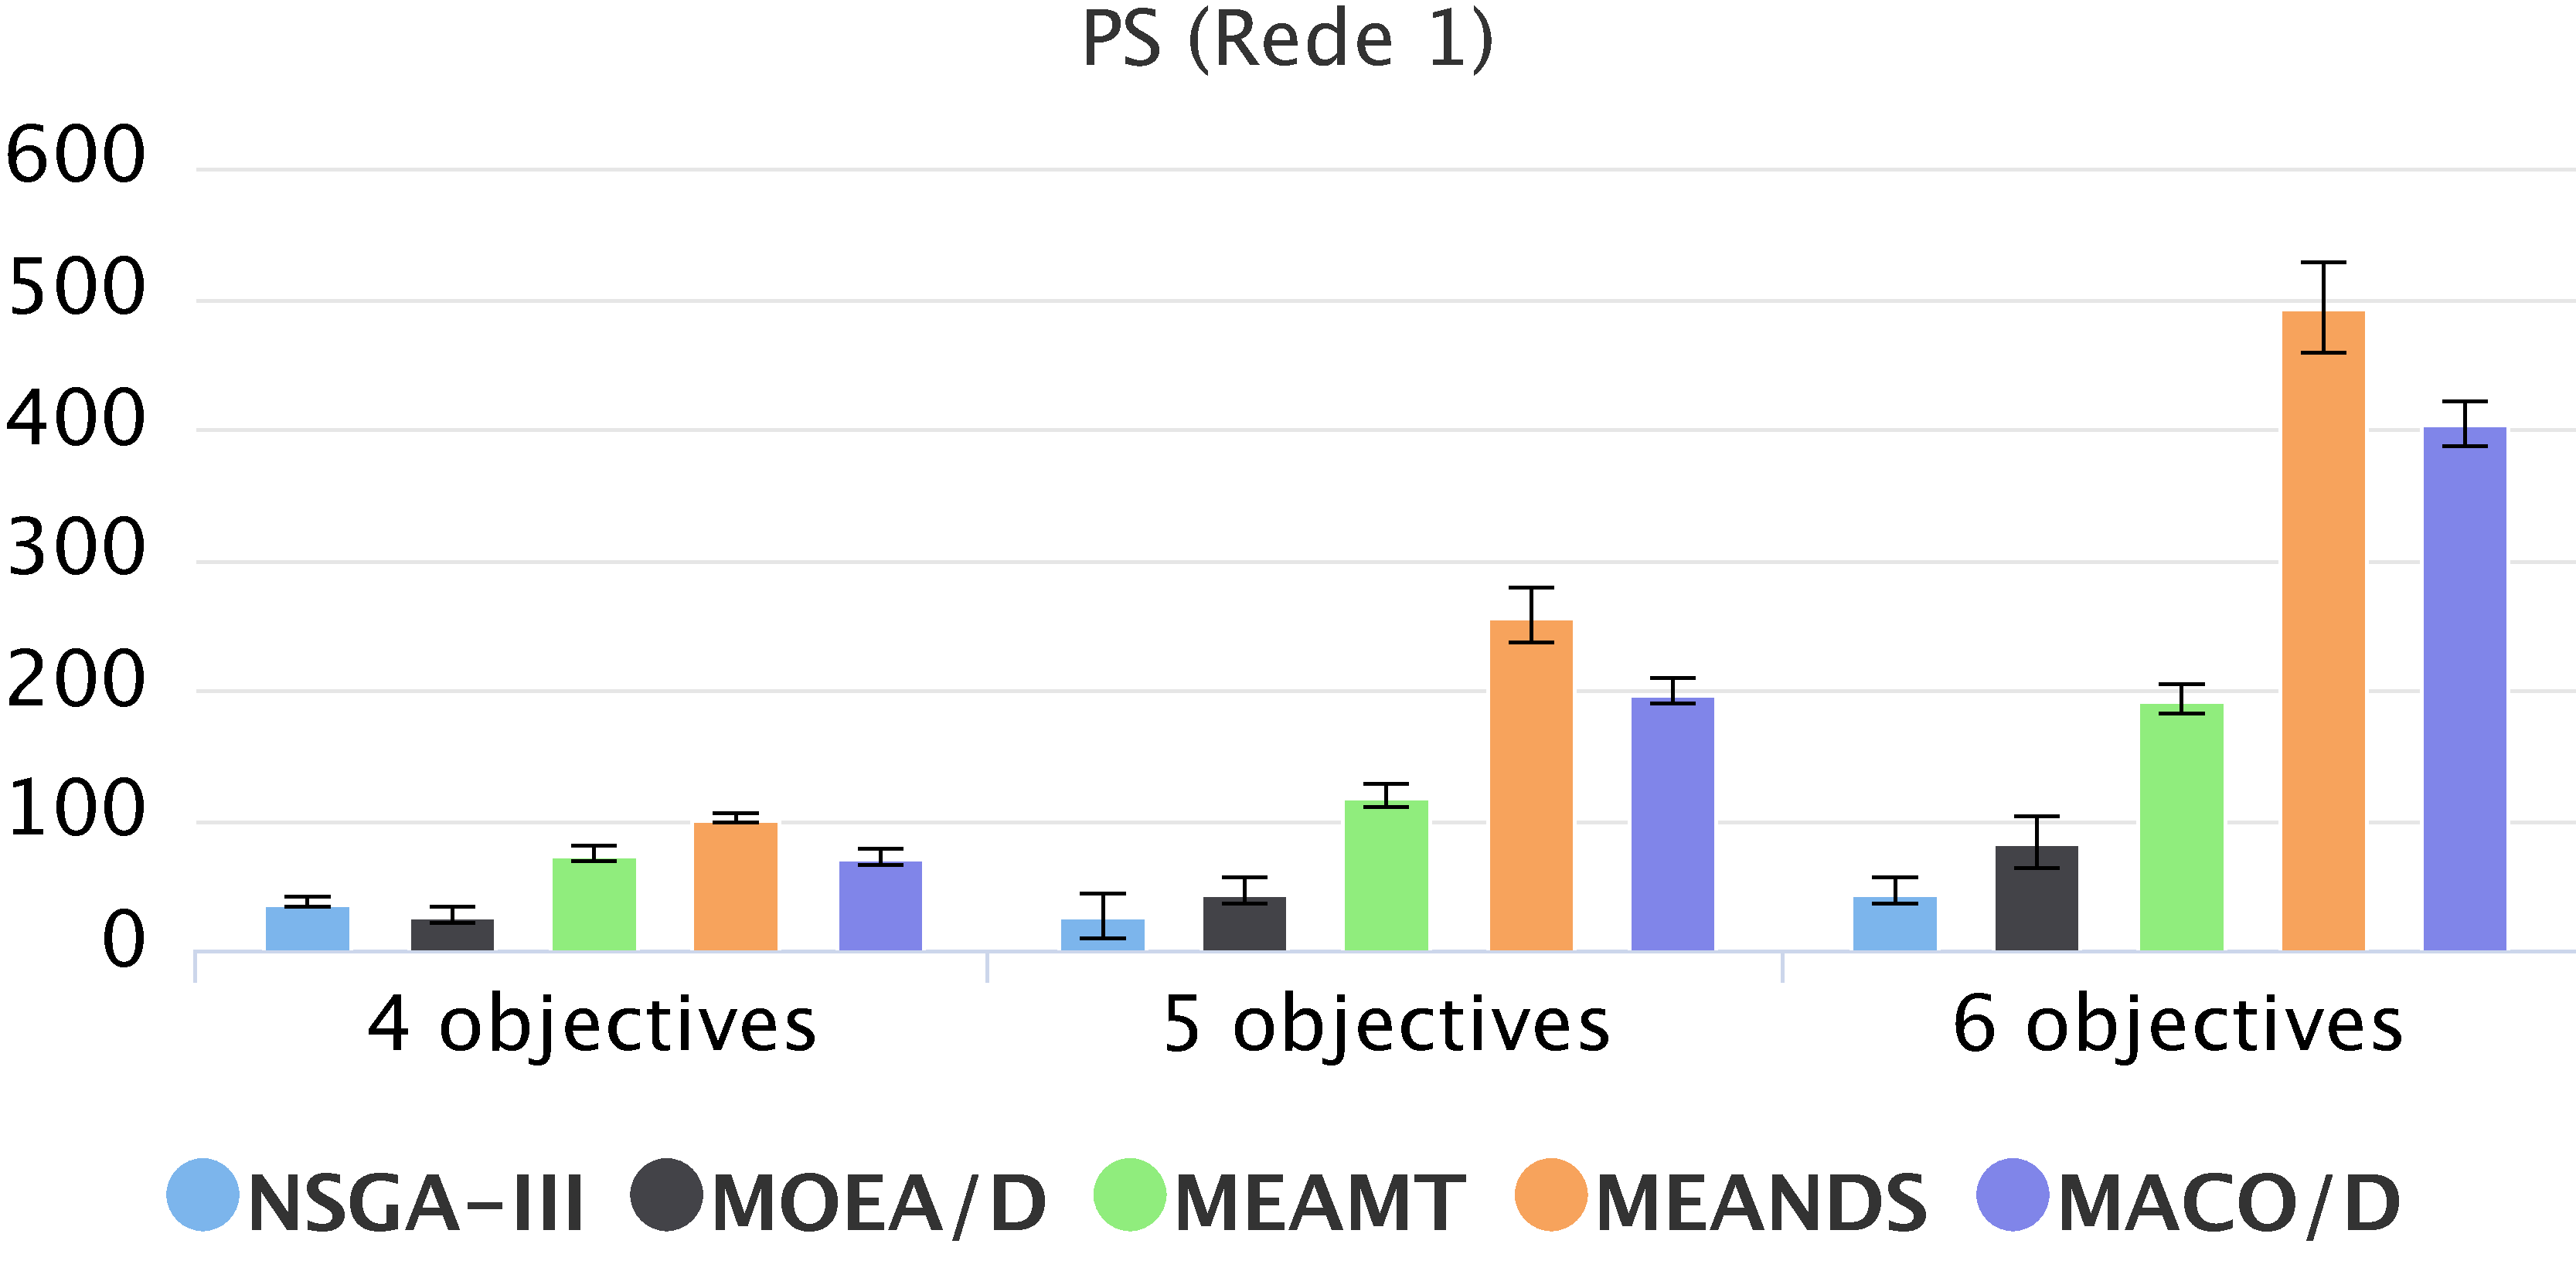
\includegraphics[width=0.5\textwidth]{cap_experimentos/figs/etapa3/ps-mrp-r1}
	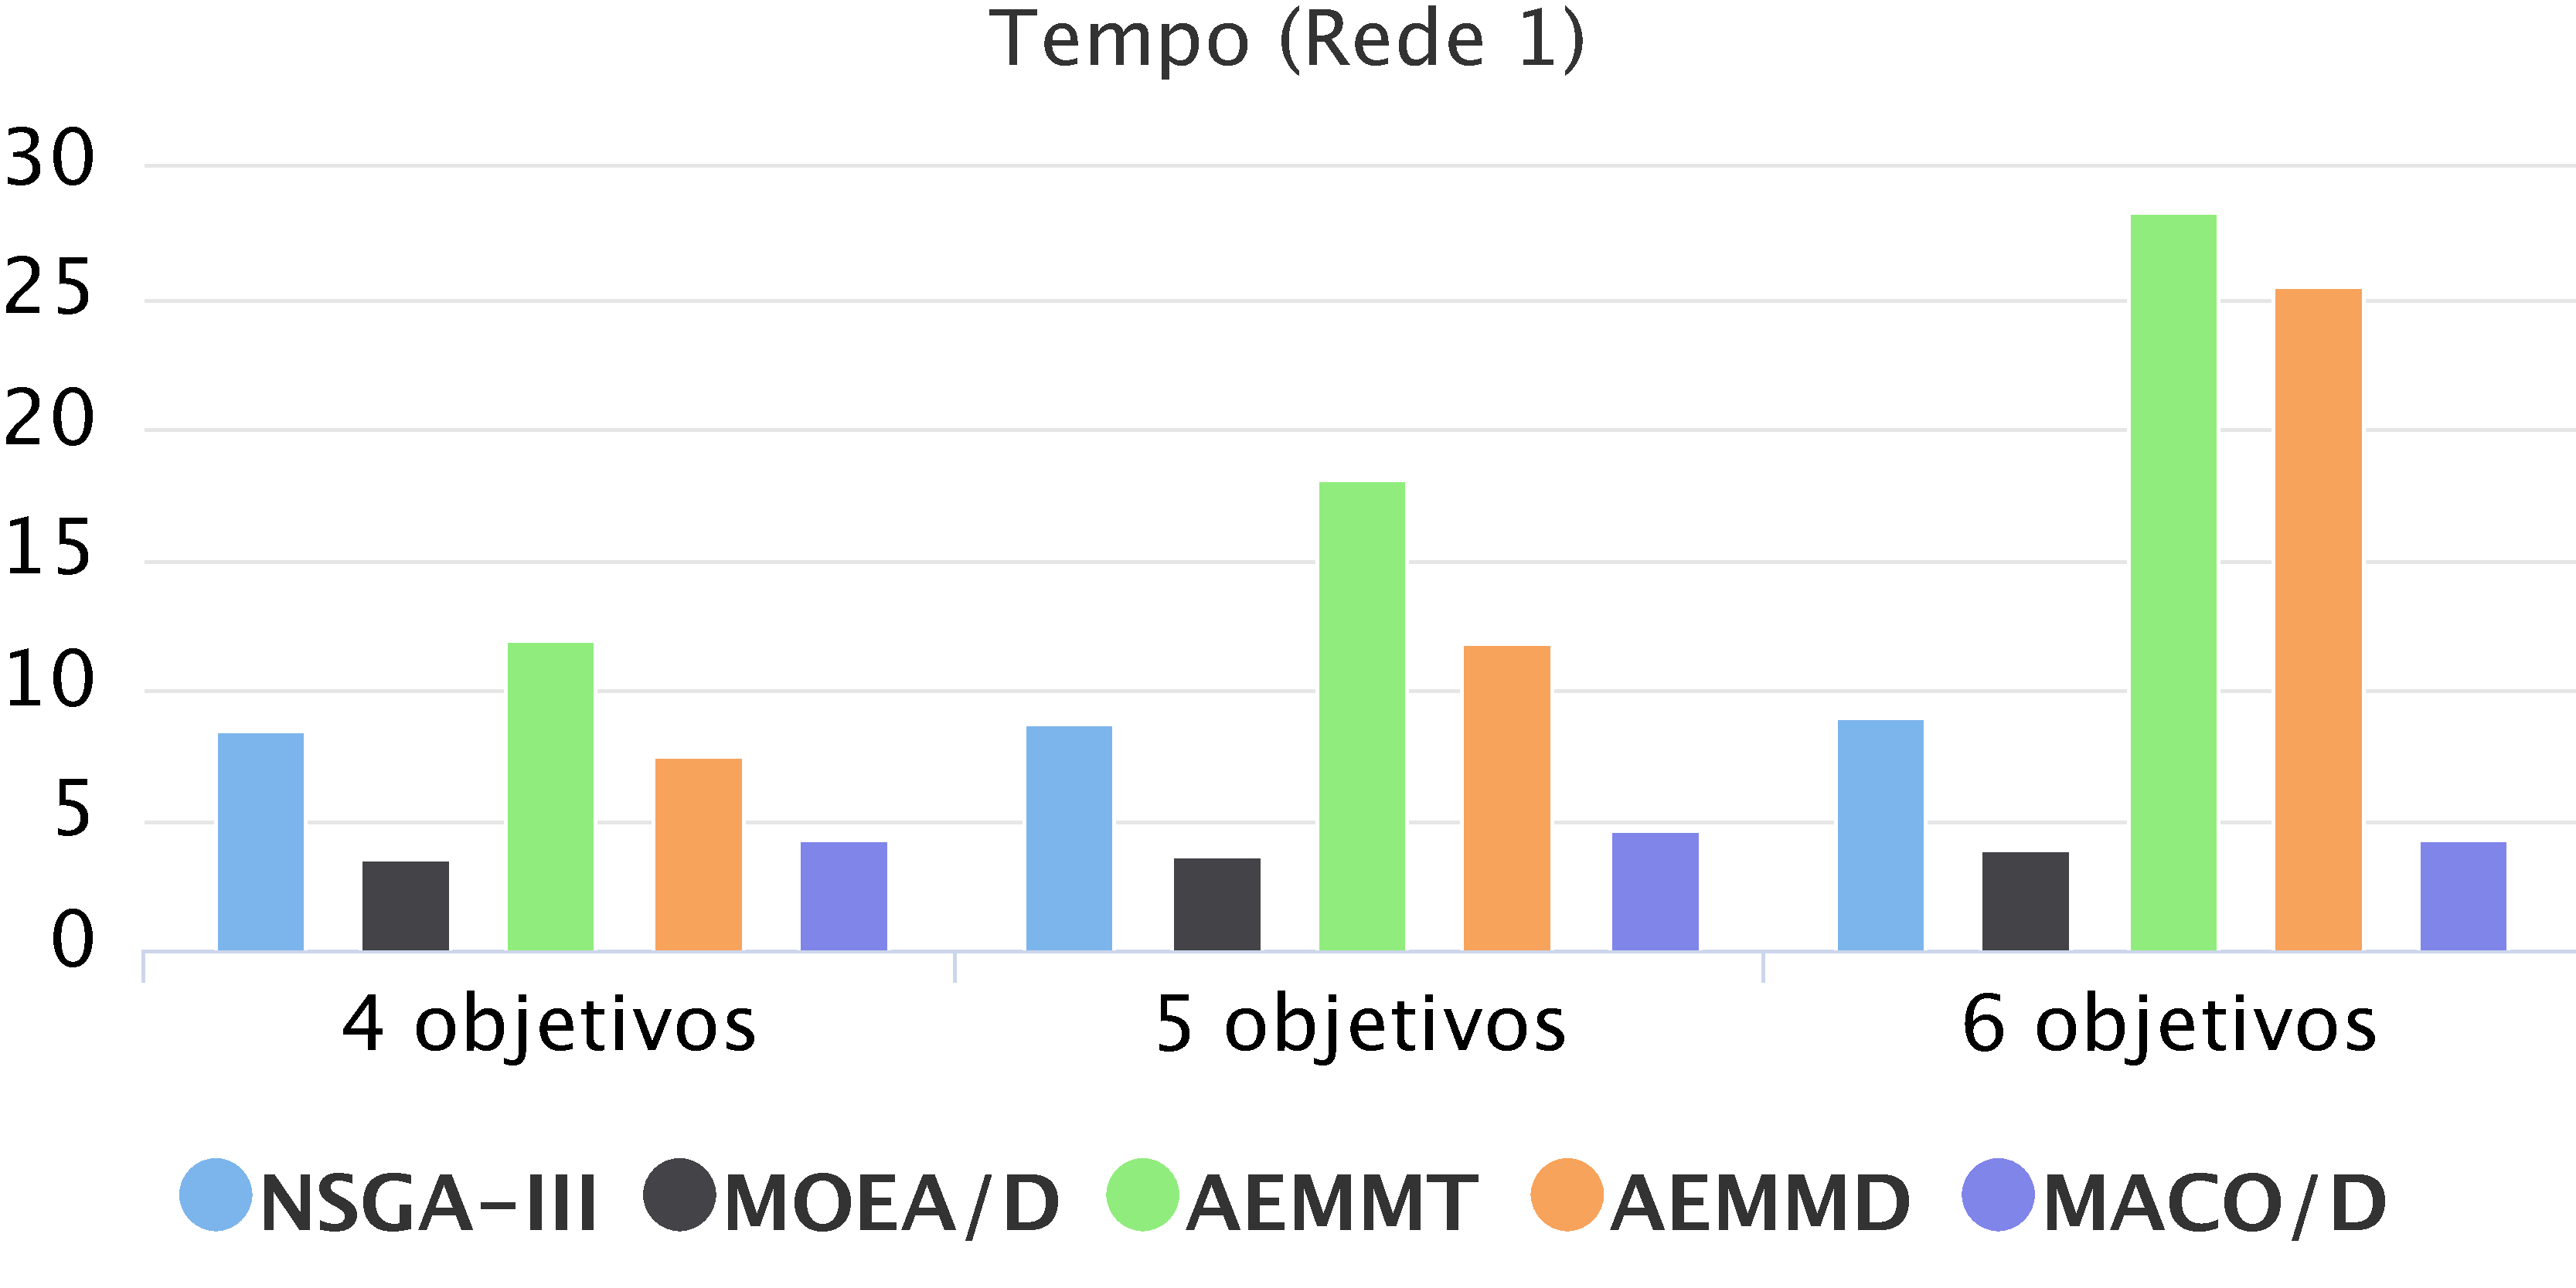
\includegraphics[width=0.5\textwidth]{cap_experimentos/figs/etapa3/time-mrp-r1}
\end{figure*}

Os gráficos correspondentes ao PRM na rede 1 (figura \ref{fig_exp3_prm_r1}) mostram uma vantagem em relação à taxa de erro pelo algoritmo AEMMD. O AEMMT e o MACO/D aparecem, respectivamente, em terceiro e quarto lugar, enquanto o MOEA/D apresenta o maior $ER$. Com relação ao $GD$, é possível observar que o MACO/D e o MOEA/D atingem desempenhos bem próximos, sendo o MACO/D o melhor entre os dois. Considerando-se o tamanho das fronteiras de Pareto encontrada ($PS$), o AEMMD é o melhor algoritmo, seguido pelo MACO/D, AEMMT, MOEA/D e NSGA-III, nessa ordem. O MACO/D e o MOEA/D são os algoritmos mais rápidos, enquanto o AEMMT e o AEMMD são os mais lentos.

\begin{figure*}[!htbp]
	\caption{Etapa 3: resultados para o PRM na rede $R_2$}
	\label{fig_exp3_prm_r2}
	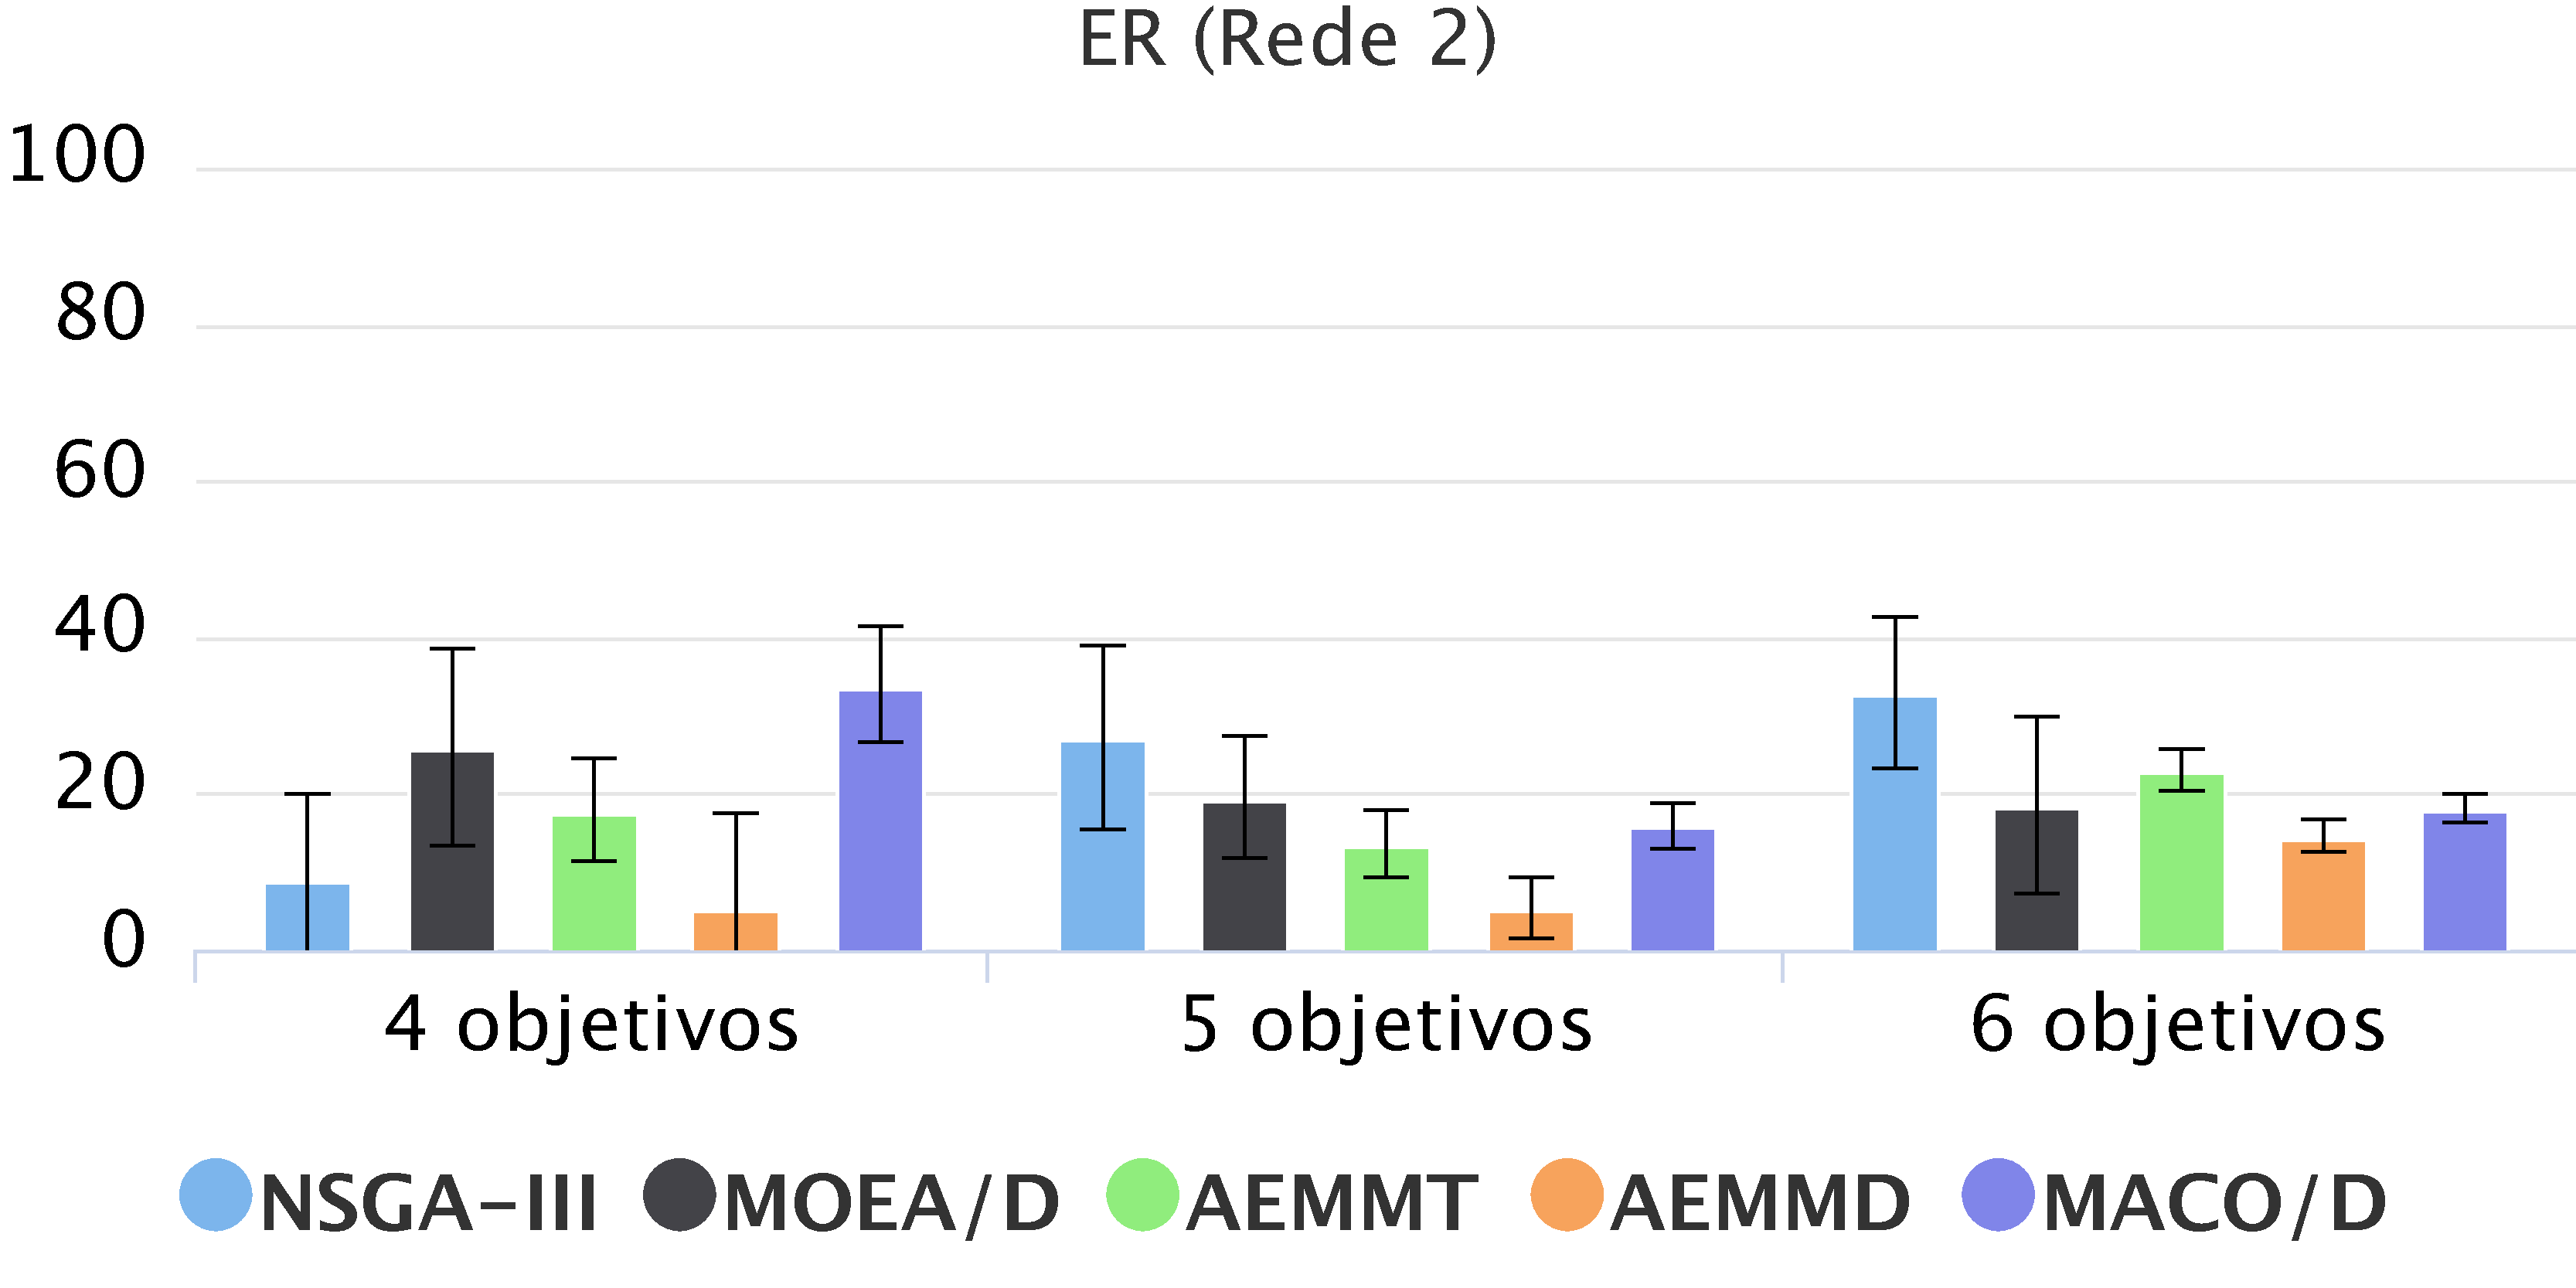
\includegraphics[width=0.5\textwidth]{cap_experimentos/figs/etapa3/er-mrp-r2}
	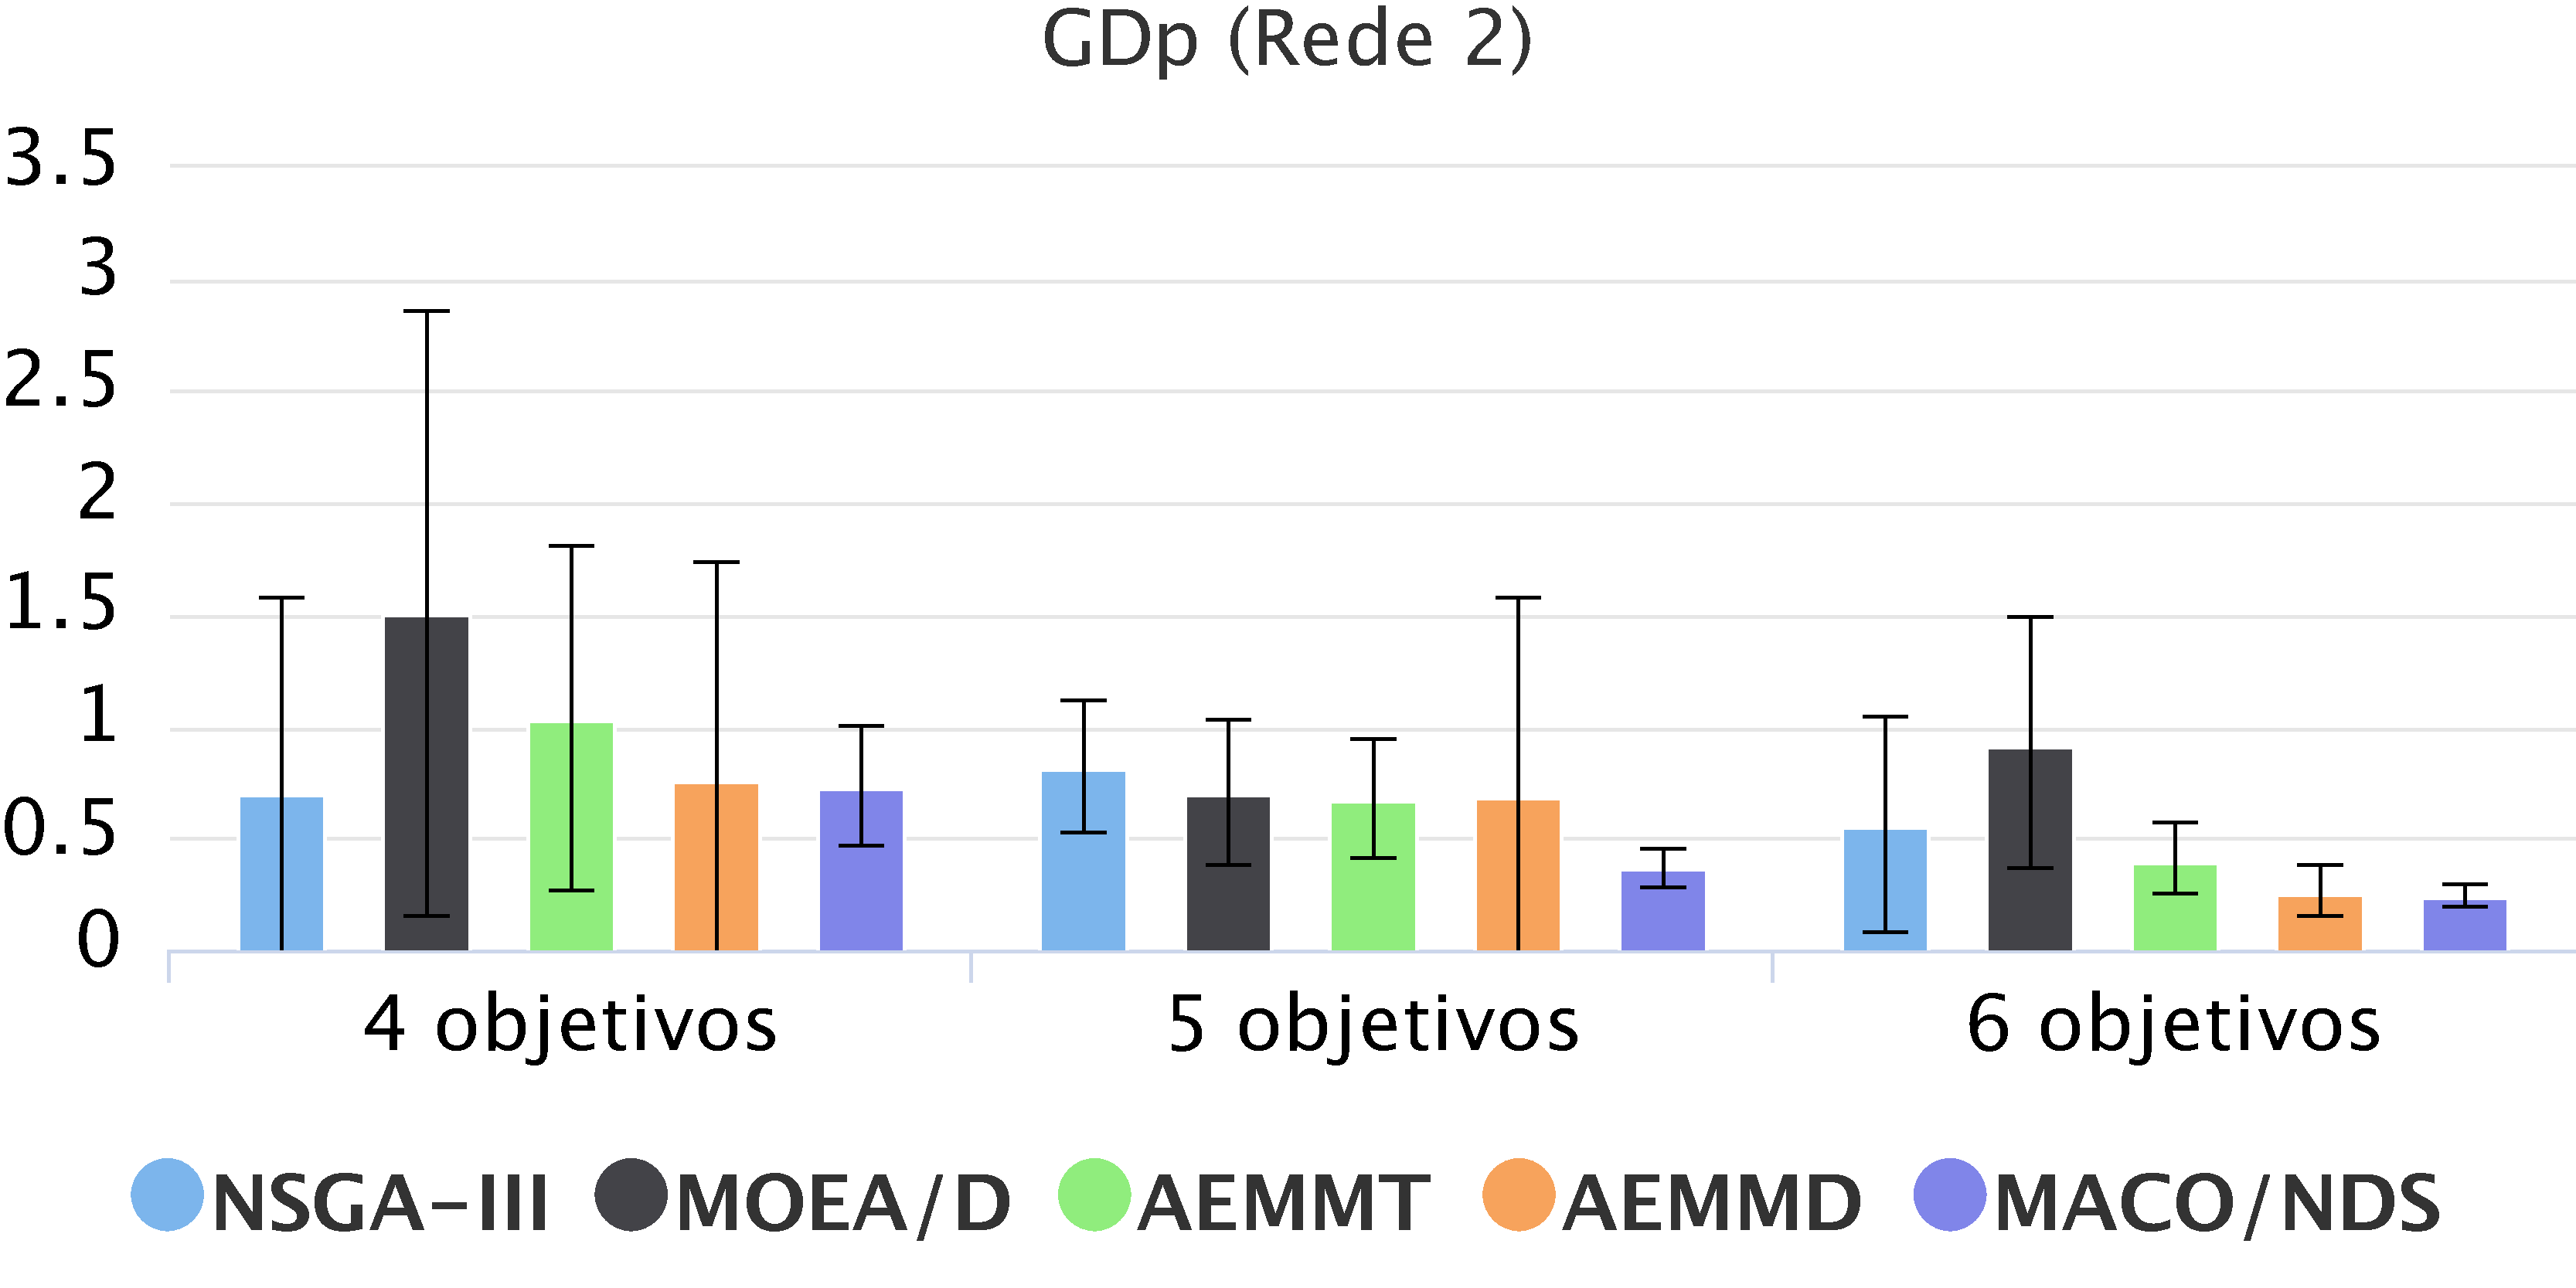
\includegraphics[width=0.5\textwidth]{cap_experimentos/figs/etapa3/gd-mrp-r2}
	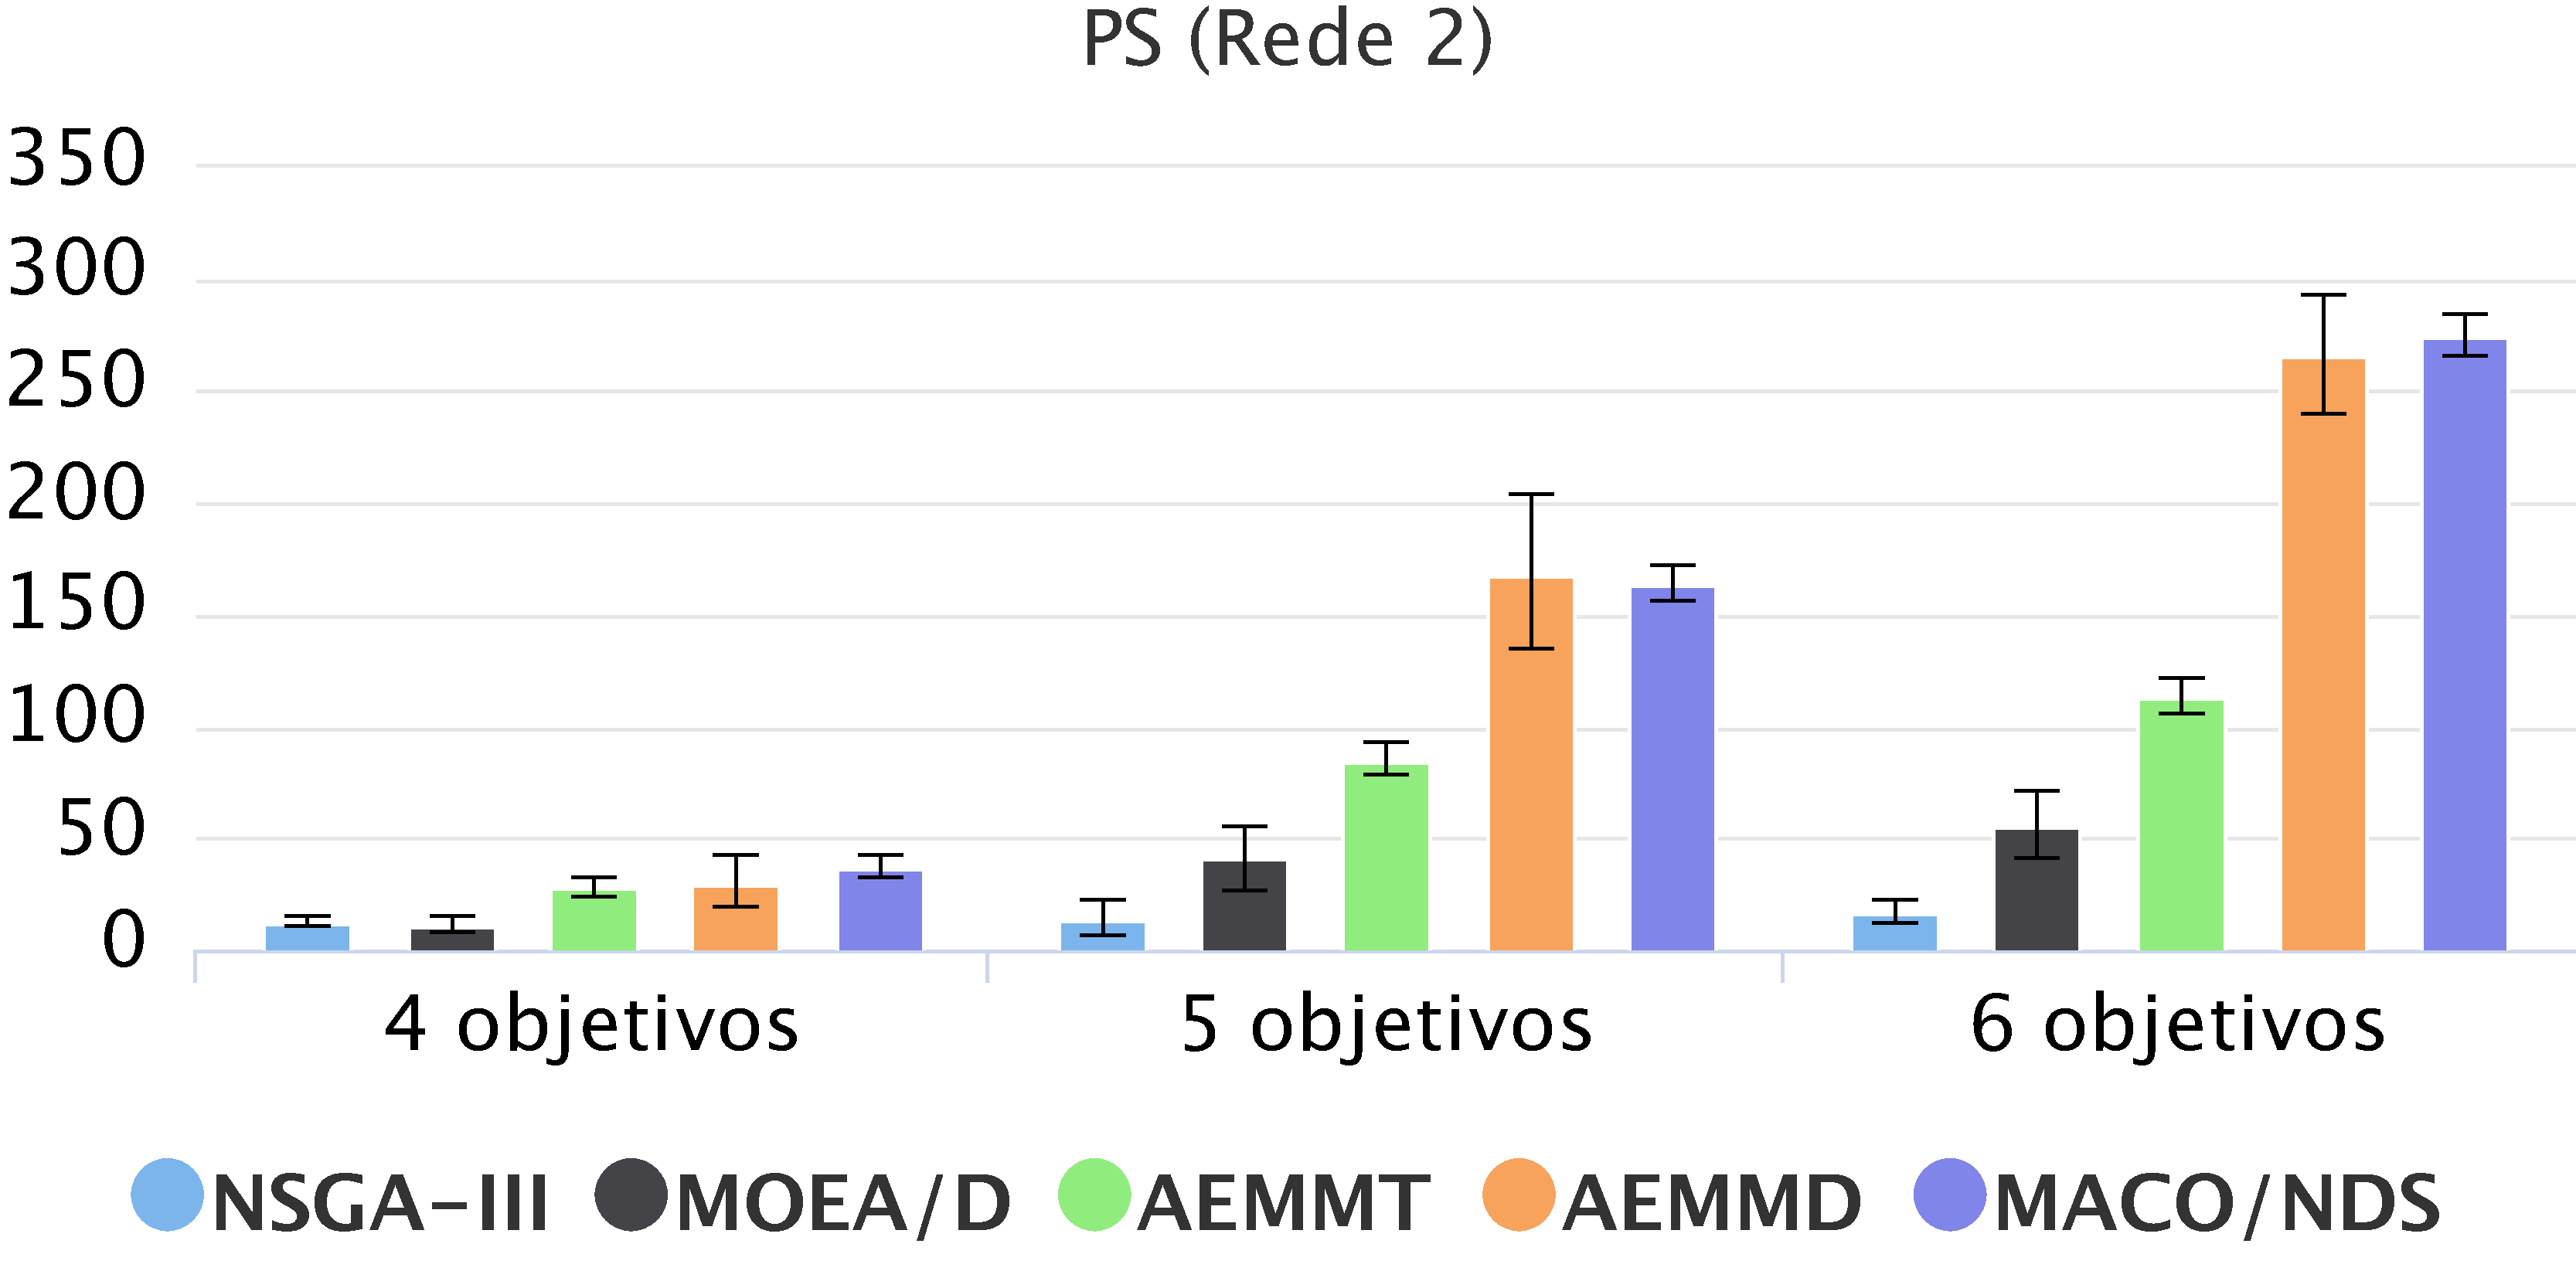
\includegraphics[width=0.5\textwidth]{cap_experimentos/figs/etapa3/ps-mrp-r2}
	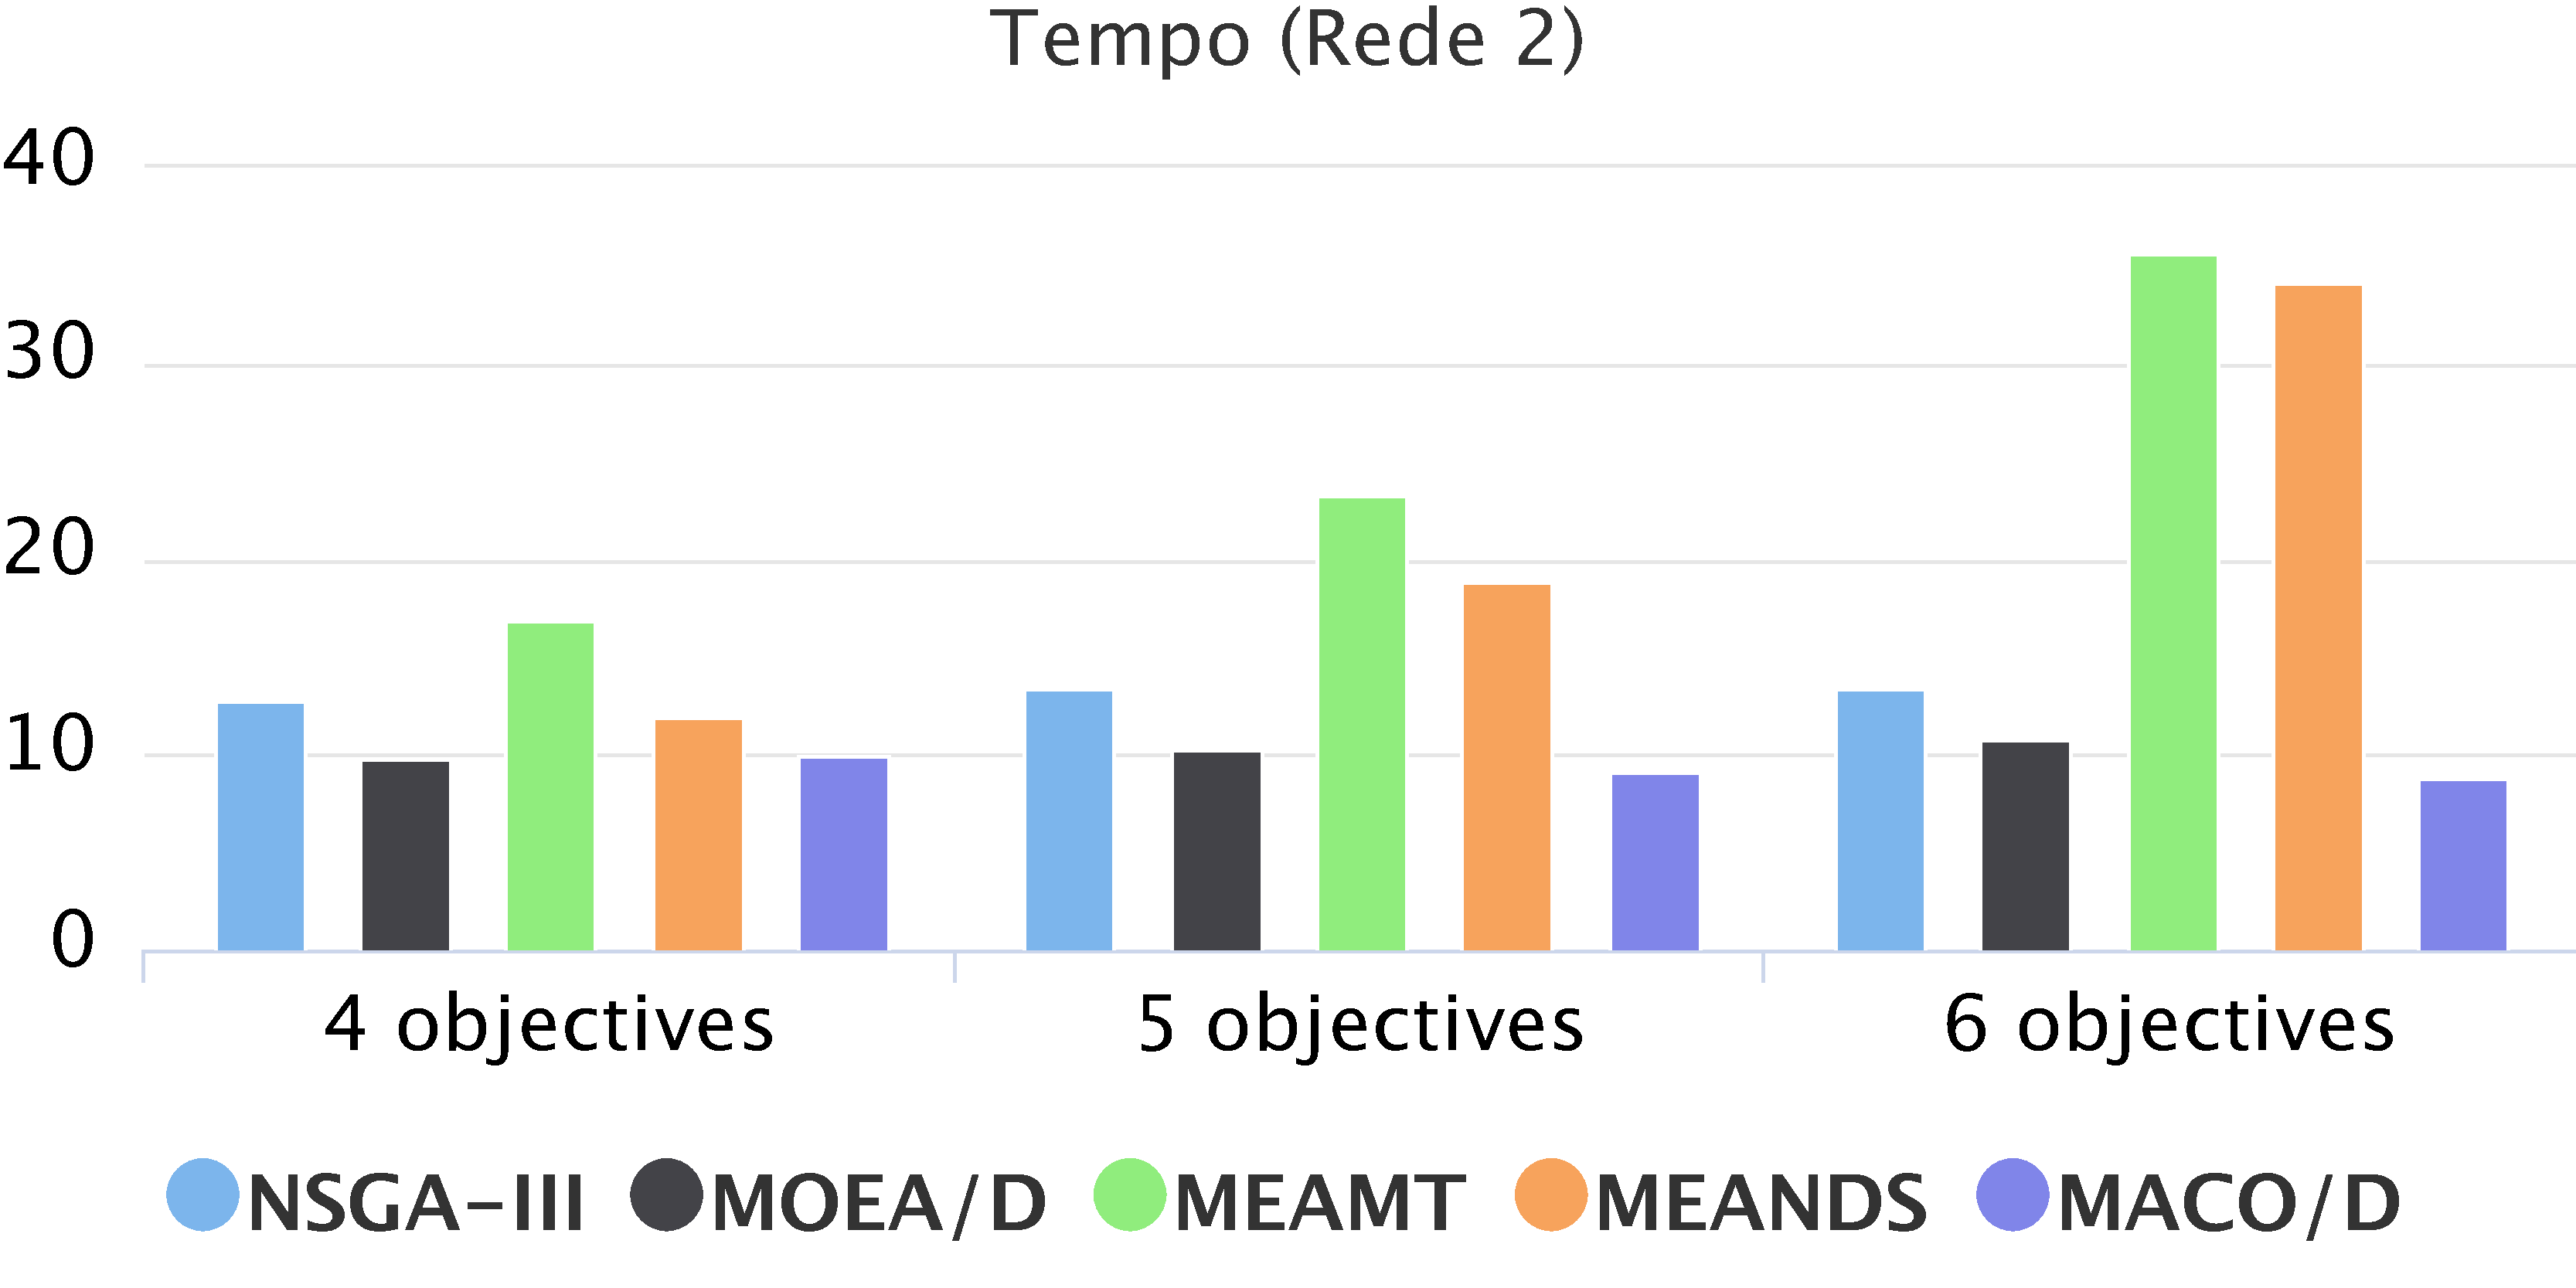
\includegraphics[width=0.5\textwidth]{cap_experimentos/figs/etapa3/time-mrp-r2}
\end{figure*}

A rede 2 (figura \ref{fig_exp3_prm_r2}), apesar de mais complexa que a primeira, apresenta comportamento bem parecido à instância anterior. O AEMMD produz as menores taxas de erro, seguido pelo AEMMT. Dentre as soluções incorretas encontradas, o MACO/D é o algoritmo que chega mais perto das soluções corretas ($GD$), sendo que os AEMMT e AEMMD conseguem resultados bem próximos. Com relação ao $PS$, os melhores valores foram encontrados pelo AEMMD, mas com vantagem muito pequena para o segundo lugar: MACO/D. Em último, aparece o NSGA-III, que é um algoritmo limitado no crescimento do Pareto. O método mais rápido é o MOEA/D e o mais lento é o AEMMT.

\begin{figure*}[!htbp]
	\caption{Etapa 3: resultados para o PRM na rede $R_3$}
	\label{fig_exp3_prm_r3}
	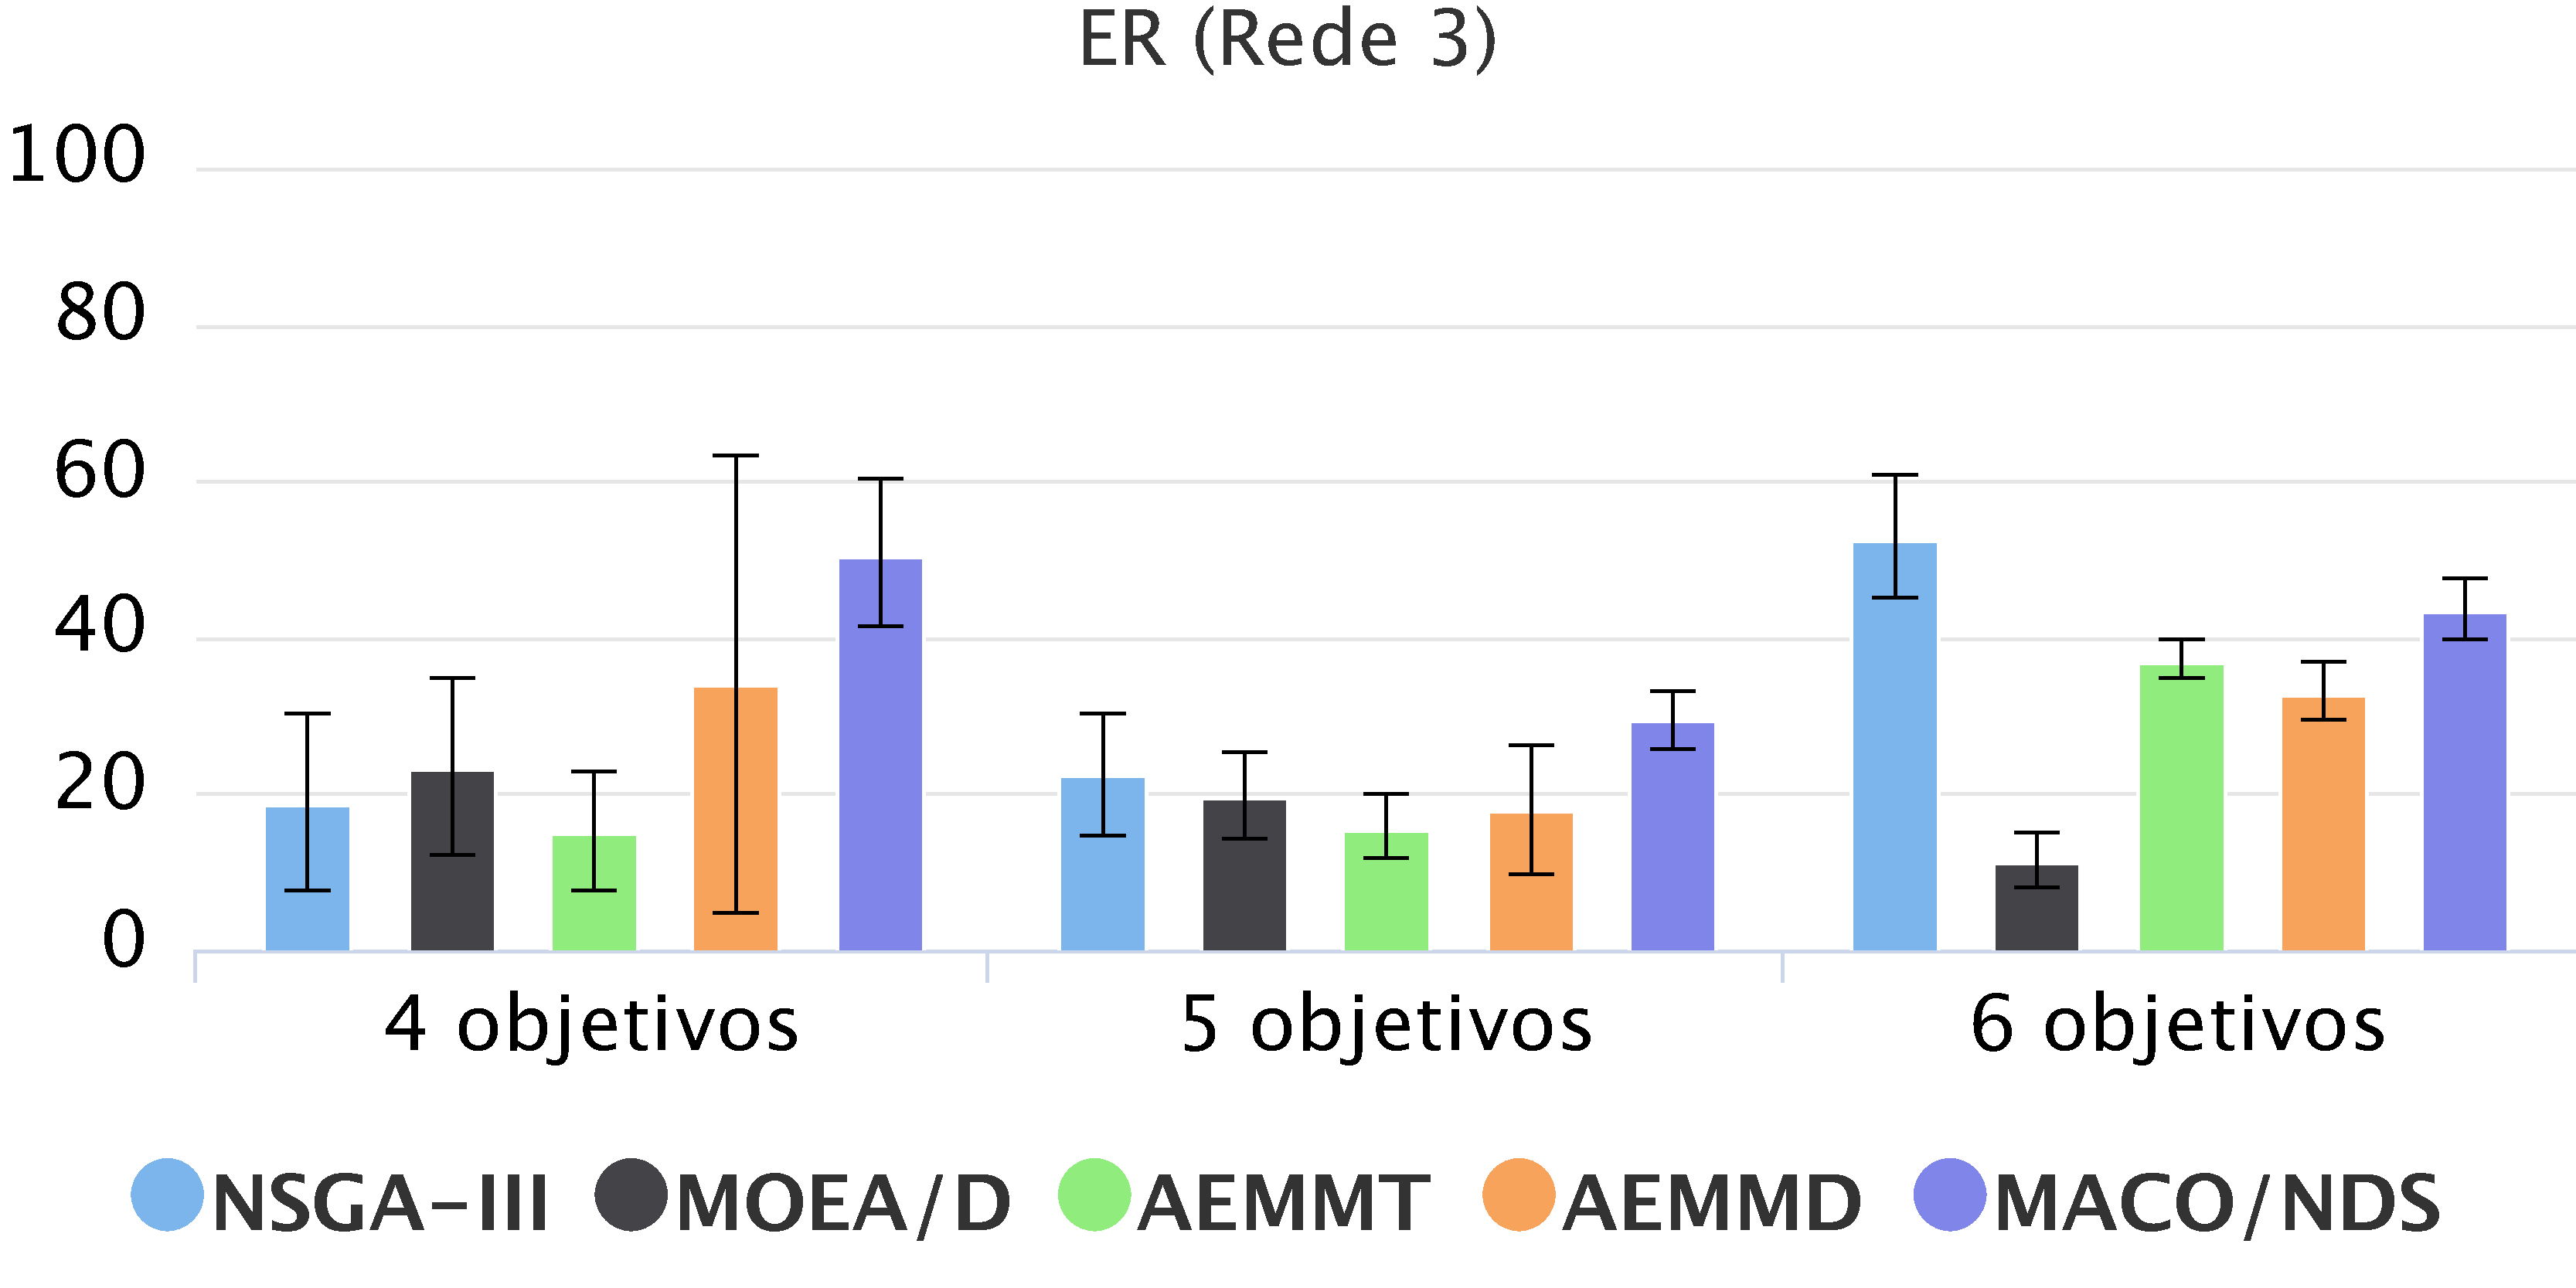
\includegraphics[width=0.5\textwidth]{cap_experimentos/figs/etapa3/er-mrp-r3}
	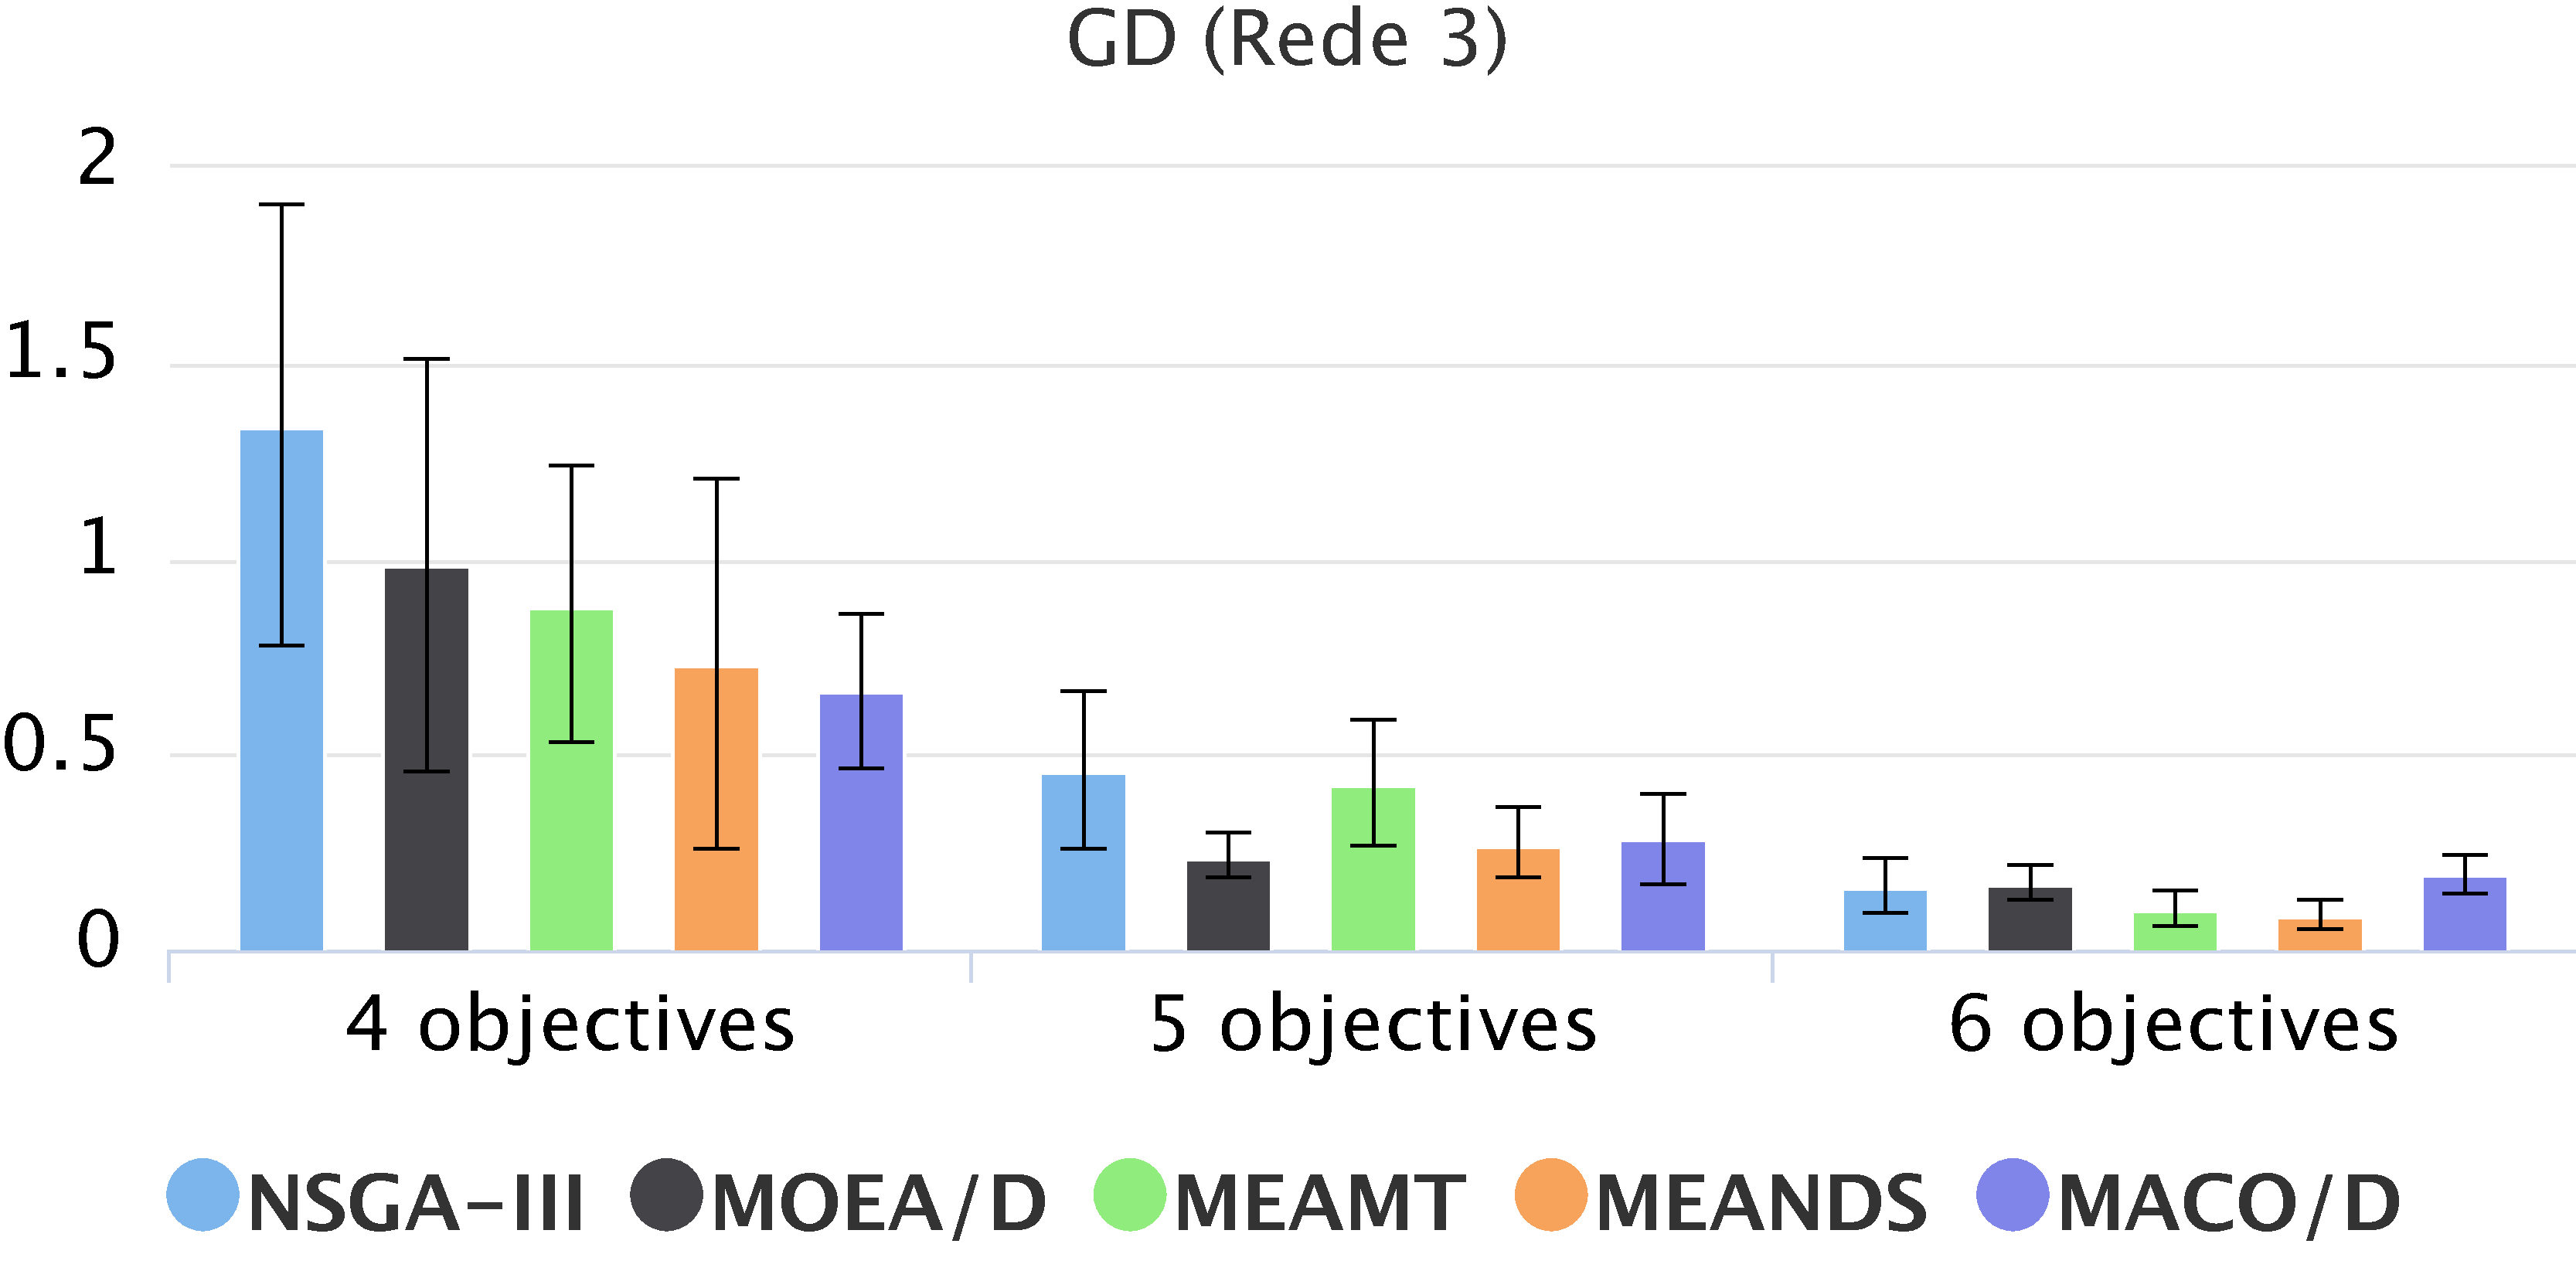
\includegraphics[width=0.5\textwidth]{cap_experimentos/figs/etapa3/gd-mrp-r3}
	\includegraphics[width=0.5\textwidth]{cap_experimentos/figs/etapa3/ps-mrp-r3}
	\includegraphics[width=0.5\textwidth]{cap_experimentos/figs/etapa3/time-mrp-r3}
\end{figure*}

No PRM aplicado à rede 3 (figura \ref{fig_exp3_prm_r3}), o AEMMT encontra as melhores taxas de erro para 4 e 5 objetivos, enquanto que para 6 objetivos, o MOEA/D consegue o melhor resultado. O NSGA-III produz o segundo menor $ER$ no problema de 4 objetivos, mas é o segundo pior no de 5 e o pior no de 6. O menor $GD$ no problema com 4 objetivos é dado pelo MACO/D, enquanto nos problemas com 5 e 6 objetivos, o AEMMT obtém o melhor $GD$. As maiores fronteiras de Pareto são encontradas pelo AEMMD e MACO/D, sendo o AEMMD o melhor entre os dois. O algoritmo mais rápido é o MACO/D, executando em tempo 5 vezes menor que o método mais lento: AEMMT.

\begin{figure*}[!htbp]
	\caption{Etapa 3: resultados agrupados para o PRM nas redes $R_1$, $R_2$ e $R_3$}
	\label{fig_exp3_prm_todos}
	\includegraphics[width=0.5\textwidth]{cap_experimentos/figs/etapa3/er-mrp-todos}
	\includegraphics[width=0.5\textwidth]{cap_experimentos/figs/etapa3/gd-mrp-todos}
	\includegraphics[width=0.5\textwidth]{cap_experimentos/figs/etapa3/ps-mrp-todos}
	\includegraphics[width=0.5\textwidth]{cap_experimentos/figs/etapa3/time-mrp-todos}
\end{figure*}

Para analisar de forma conjunta os resultados das três redes, na figura \ref{fig_exp3_prm_todos} compila-se todos os experimentos através da média aritmética dos resultados. De maneira geral, o NSGA-III consegue soluções de qualidade razoável, mas apresenta baixo $PS$ e apesar de não ser um algoritmo lento, também não é o mais rápido. O MOEA/D obtém as melhores taxas de erro no problema de seis objetivos e tem desempenho razoável nos problemas de 4 e 5 objetivos, seu $GD$ é levemente mais alto que os demais métodos e seu $PS$ é baixo. A velocidade de execução do MOEA/D é tão boa quanto a do MACO/D, juntos são os dois algoritmos mais rápidos, tornando o MOEA/D uma boa opção se o objetivo da busca é conseguir uma baixa taxa de erro em um curto tempo de execução, sem se preocupar com o $PS$. Os melhores resultados foram obtidos pelo AEMMD e o método proposto: MACO/D. Com relação ao erro, o AEMMD consegue as melhores taxas, o MACO/D não fica muito atrás. Analisando o $GD$, observa-se que não há muita diferença entre os dois métodos, mas o MACO/D gera melhores soluções que o AEMMD, além disso, o desvio padrão do MACO/D é consideravelmente menor, o que o revela ser um método mais estável no que se refere à qualidade das soluções. O AEMMD produz as maiores fronteiras de Pareto, mas o MACO/D apresenta resultado bem próximo. O mais interessante nesta análise é o tempo de execução, por mais que o AEMMD gere soluções razoavelmente melhores que o MACO/D considerando as métricas $ER$ e $GD$, o segundo é consideravelmente mais rápido, chegando a executar em quase 5 vezes menos tempo. Considerando o fato de que o PRM é um problema sensível ao tempo de execução, pelo menos nos cenários analisados, o MACO/D é a melhor opção entre os algoritmos testados.

A primeira diferença que se nota entre os resultados dos dois problemas é o tempo de execução do algoritmo proposto, o MACO/D. considerando os gráficos da figura \ref{fig_exp3_pmm_todos}, o MACO/D é o segundo algoritmo mais lento e seu tempo de execução está altamente relacionado ao número de objetivos. Na figura \ref{fig_exp3_prm_todos}, que representa o comportamento geral dos algoritmos no PRM, vê-se o oposto: o MACO/D é o algoritmo mais rápido e seu tempo de execução se mantém estável independente da formulação de objetivos. O processo de maior custo computacional no MACO/D é a atualização dos feromônios, onde é necessário recalcular o conjunto de soluções não-dominadas $nd$. A cada iteração, para toda solução criada, é necessário passar por todos elementos em $nd$ verificando a relação de não-dominância. Naturalmente, quanto maior o conjunto $nd$ mais caro se torna o processo. No PRM, foram encontradas fronteiras de Pareto de tamanho razoavelmente pequenos, todas com menos de 350 elementos, ou seja, foi necessário, para cada solução criada, fazer no máximo 350 comparações. No caso do PMM, as fronteiras de Pareto são muito grandes, no problema com 6 objetivos e 50 itens, por exemplo, a cardinalidade do conjunto $nd$ chega a ser maior que 4500. Quanto maior a quantidade de objetivos do problema, maior o número de soluções no Pareto e mais lento será a classificação de soluções não dominadas. Se o conjunto $nd$ é pequeno até mesmo para a maior quantidade de objetivos (caso do PRM), o processo será rápido e o tempo de execução não será muito diferente entre as formulações de objetivos. Por outro lado, se a cardinalidade de $nd$ é muito grande e cresce muito com o aumento da quantidade de objetivos, o tempo necessário para se atualizar os feromônios será muito alto e terá grande variação conforme a formulação de objetivos.

A fim de melhor comparar o MACO/D aos algoritmos AEMMT e AEMMD realizou-se o teste de hipótese z-teste com 5\% de significância ($\alpha=0.05$). Os resultados são mostrados nas tabelas \ref{tab_ztest_meamt} e \ref{tab_ztest_meams}. Em ambas as tabelas, uma célula de fundo verde representa uma ocasião onde o MOACS obteve melhor resultado que seu adversário, vermelho significa pior e branco empate.

\begin{table}[htb]
	\centering
	\def\arraystretch{1.0}
	\caption{Testes de hipótese para: MACO/D vs. AEMMT nos problemas PMM and PRM}
	\label{tab_ztest_meamt}
	\begin{tabular}{llllllllll}
		& \multicolumn{3}{l}{\textbf{4 objectives}} & \multicolumn{3}{l}{\textbf{5 objectives}} & \multicolumn{3}{l}{\textbf{6 objectives
		}} \\
		\textbf{Instance} & \textbf{ER} & \textbf{GD} & \textbf{PS} & \textbf{ER} & \textbf{GD} & \textbf{PS} & \textbf{ER} & \textbf{GD} & \textbf{PS} \\ \hline
		30 items & \cellcolor{white} $=$ & \cellcolor{table-green} $<$ & \cellcolor{table-green} $>$ & \cellcolor{table-red} $>$ & \cellcolor{table-green} $<$ & \cellcolor{table-green} $>$ & \cellcolor{table-red} $>$ & \cellcolor{table-green} $<$ & \cellcolor{table-green} $>$ \\
		40 items & \cellcolor{table-green} $<$ & \cellcolor{table-green} $<$ & \cellcolor{table-green} $>$ & \cellcolor{table-green} $<$ & \cellcolor{table-green} $<$ & \cellcolor{table-green} $>$ & \cellcolor{table-red} $>$ & \cellcolor{table-green} $<$ & \cellcolor{table-green} $>$ \\
		50 items & \cellcolor{table-green} $<$ & \cellcolor{white} $=$ & \cellcolor{table-green} $>$ & \cellcolor{table-green} $<$ & \cellcolor{table-green} $<$ & \cellcolor{table-green} $>$ & \cellcolor{table-red} $>$ & \cellcolor{table-green} $<$ & \cellcolor{table-green} $>$ \\  \hline 
		Rede 1 & \cellcolor{table-red} $>$ & \cellcolor{table-green} $<$ & \cellcolor{table-red} $<$ & \cellcolor{table-red} $>$ & \cellcolor{table-green} $<$ & \cellcolor{table-green} $>$ & \cellcolor{table-red} $>$ & \cellcolor{table-green} $<$ & \cellcolor{table-green} $>$ \\
		Rede 2 & \cellcolor{table-red} $>$ & \cellcolor{table-green} $<$ & \cellcolor{table-green} $>$ & \cellcolor{table-red} $>$ & \cellcolor{table-green} $<$ & \cellcolor{table-green} $>$ & \cellcolor{table-green} $<$ & \cellcolor{table-green} $<$ & \cellcolor{table-green} $>$ \\
		Rede 3 & \cellcolor{table-red} $>$ & \cellcolor{table-green} $<$ & \cellcolor{table-red} $<$ & \cellcolor{table-red} $>$ & \cellcolor{table-green} $<$ & \cellcolor{table-green} $>$ & \cellcolor{table-red} $>$ & \cellcolor{table-red} $>$ & \cellcolor{table-green} $>$ \\  \hline 
	\end{tabular}
\end{table}

\begin{table}[htb]
	\centering
	\def\arraystretch{1.0}
	\caption{Testes de hipótese para: MACO/D vs. AEMMD nos problemas PMM and PRM}
	\label{tab_ztest_meams}
	\begin{tabular}{llllllllll}
		& \multicolumn{3}{l}{\textbf{4 objectives}} & \multicolumn{3}{l}{\textbf{5 objectives}} & \multicolumn{3}{l}{\textbf{6 objectives
		}} \\
		\textbf{Instance} & \textbf{ER} & \textbf{GD} & \textbf{PS} & \textbf{ER} & \textbf{GD} & \textbf{PS} & \textbf{ER} & \textbf{GD} & \textbf{PS} \\ \hline
		30 items & \cellcolor{table-green} $<$ & \cellcolor{table-green} $<$ & \cellcolor{table-green} $>$ & \cellcolor{table-green} $<$ & \cellcolor{table-red} $>$ & \cellcolor{table-green} $>$ & \cellcolor{table-green} $<$ & \cellcolor{table-red} $>$ & \cellcolor{table-green} $>$ \\
		40 items & \cellcolor{table-green} $<$ & \cellcolor{table-red} $>$ & \cellcolor{table-green} $>$ & \cellcolor{table-green} $<$ & \cellcolor{table-red} $>$ & \cellcolor{table-green} $>$ & \cellcolor{table-green} $<$ & \cellcolor{table-red} $>$ & \cellcolor{table-green} $>$ \\
		50 items & \cellcolor{table-green} $<$ & \cellcolor{table-green} $<$ & \cellcolor{table-green} $>$ & \cellcolor{table-green} $<$ & \cellcolor{table-green} $<$ & \cellcolor{table-green} $>$ & \cellcolor{table-green} $<$ & \cellcolor{table-green} $<$ & \cellcolor{table-green} $>$ \\  \hline 
		Rede 1 & \cellcolor{table-red} $>$ & \cellcolor{table-green} $<$ & \cellcolor{table-red} $<$ & \cellcolor{table-red} $>$ & \cellcolor{table-green} $<$ & \cellcolor{table-red} $<$ & \cellcolor{table-red} $>$ & \cellcolor{table-green} $<$ & \cellcolor{table-red} $<$ \\
		Rede 2 & \cellcolor{table-red} $>$ & \cellcolor{white} $=$ & \cellcolor{table-green} $>$ & \cellcolor{table-red} $>$ & \cellcolor{table-green} $<$ & \cellcolor{table-red} $<$ & \cellcolor{table-red} $>$ & \cellcolor{table-green} $<$ & \cellcolor{table-green} $>$ \\
		Rede 3 & \cellcolor{table-red} $>$ & \cellcolor{table-green} $<$ & \cellcolor{table-red} $<$ & \cellcolor{table-red} $>$ & \cellcolor{white} $=$ & \cellcolor{table-red} $<$ & \cellcolor{table-red} $>$ & \cellcolor{table-red} $>$ & \cellcolor{table-red} $<$ \\  \hline 
	\end{tabular}
\end{table}

No PMM, se o tempo de execução é uma preocupação, a melhor alternativa é o algoritmo MOEA/D, que executa em tempo recorde e produz bons resultados. Se a rapidez do algoritmo não é tão importante e deseja-se encontrar um conjunto de soluções mais próximo do Pareto real, o MACO/D é o algoritmo mais indicado. No PRM, o método que representa melhor relação entre qualidade e tempo é o MACO/D, mas se tempo não é importante, o AEMMD pode ser preferível. Ao mesmo tempo, seria interessante testar se, dada a mesma quantidade de tempo, o MACO/D não supera o AEMMD.

\section{Etapa 4: Análise com hipervolume}
\label{section_experimentos_etapa4}

A fim de testar propriamente o comportamento dos algoritmos em espaços de busca mais complexos que os utilizados nos experimentos das etapas 1 e 3, lançou-se mão de duas novas redes (redes 4 e 5) e duas novas instâncias do problema da mochila (100 e 200 itens). Como não é possível extrair Paretos estáveis para as redes $R_3$, $R_4$ e $R_5$, nem para os problemas da mochila com 50, 100 e 200 itens, não é interessante basear-se em métricas dependentes de tais Paretos para se tirar conclusões. Por isso, nesta etapa, testa-se unicamente as métrica hiper-volume e tempo, independentes do Pareto.

O hiper-volume, junto ao \textit{inverse generational distance} $(IDG)$, são as métricas mais utilizadas na literatura para se avaliar algoritmos many-objectives. O hiper-volume, como explicado no início deste capítulo, calcula o volume da figura geométrica formada pelas distâncias das soluções a um ponto de referência pré-definido. Os pontos de referência utilizados em cada cenário são apresentados na tabela \ref{table_exp4_pts_referencia}.

Neste conjunto de experimentos, assim como na etapa 3, comparou-se apenas os cenários many-objectives, com 4, 5 e 6 objetivos. Por esse motivo, ficaram de fora dos testes os algoritmos clássicos NSGA-II e SPEA2. Em contra-partida incluiu-se 3 novos métodos many-objectives na comparação: SPEA2-SDE (AG), MOACS (ACO) e MOEA/D-ACO (ACO). Os parâmetros utilizados para cada método podem ser encontrados na tabela \ref{table_exp4_params}.

\begin{table}[!htbp]
	\caption{Parâmetros utilizados para o PRM e o PMM na etapa 4 de experimentos.}
	\label{table_exp4_params}
	\begin{center}
		\begin{tabular}{c|r|r}
			\textbf{Parâmetro} & \textbf{PRM} &  \textbf{PMM} \\ %\hline
			\hline
			Tamanho da população               &    90 &      150 \\ %\hline
			Número de comparações        &   9000 &      15000 \\ %\hline
			Taxa de crossover                & 100\% &    100\% \\ %\hline
			Taxa de mutação                 &  20\% &      5\% \\ %\hline
			Tamanho da vizinhança (MOEA/D e MOEA/D-ACO)    &    10 &       10 \\ %\hline
			Tamanho das tabelas (MEAMT)   &    30 &       50 \\ %\hline
			Tamanho da tabela de dominância (MEAMT) &    90 &      150 \\ %\hline
			Número de divisões (NSGA-III)&     8 &        8 \\ %\hline
			$\alpha, \beta, \rho$ (ACO's)& 1, 2, 0.3 & 1, 4.3, 0.3 \\ %\hline
			Intervalo de valores para os feromônios (ACO's)& [0.1, 0.9] & [0.1, 0.9] \\ %\hline
			$\delta$ (MOEA/D-ACO)& 0.2 & 0.2 \\ %\hline
			Número de formigas e grupos (MOEA/D-ACO)*& 6 & variável \\ %\hline
			Número de grupos de formigas (MOEA/D-ACO)*& 3 & 3 \\ %\hline
			Taxa de elitismo (MOEA/D-ACO)& 0.9 & 0 \\ %\hline
			Tamanho das amostras (MACO/D)& 10 & 10 \\  %\hline
			Tamanho do grupo de estruturas ativas (MACO/D)& 5 & 5 \\
			\hline
		\end{tabular}
	\end{center}
\end{table}

Sobre os parâmetros marcados com ``*'' na tabela \ref{table_exp4_params}, a quantidade de formigas depende do parâmetro $H$, do artigo original do algoritmo \cite{ke2013}, enquanto o tamanho dos grupos depende de outro parâmetro, $K$, também descrito no mesmo artigo. Ambos os parâmetros $H$ e $K$ servem como guia para gerar os pesos aleatórios das formigas e dos grupos, quanto maior o valor de $H$, maior será o número de formigas, o mesmo vale para $K$ e a quantidade de grupos. De toda maneira, o número de iterações no laço principal é ajustado para que sempre se tenha o mesmo número de comparações (9000 no PRM e 15000 no PMM). Os valores de $H$ usados no PMM foram: $H=8$ para 4 objetivos, $H=6$ para 5 objetivos e $H=5$ para 6 objetivos.

Com relação aos algoritmos NSGA-III e SPEA2-SDE, na etapa 4, tomou-se uma outra atitude em relação às limitações no tamanho do Pareto. Ao invés de impedir o conjunto de soluções não-dominadas de crescerem além do tamanho máximo da população, ajustou-se esse limite para coincidi-lo com o tamanho médio dos Paretos encontrados pelos algoritmos que retornaram os maiores conjuntos de soluções. Dessa forma, ambos NSGA-III e SPEA2-SDE podem encontrar Paretos tão grandes quanto os demais algoritmos. A tabela \ref{table_exp4_pts_referencia} mostra os limites utilizados para cada cenário de teste.

\begin{table}[!htbp]
	\centering
	\caption{Ponto de referência e limitações no tamanho do Pareto usados para cada cenário de teste}
	\label{table_exp4_pts_referencia}
	\begin{tabular}{clll}
		\textbf{Instância}                                                       & \textbf{Obj.} & \textbf{Ponto de referência}                          & \textbf{Limite} \\ \hline
		\multirow{3}{*}{\begin{tabular}[c]{@{}c@{}}PMM\\ 50 itens\end{tabular}}  & 4             & {[}-15665, -17464, -19122, -16978{]}                   & 600             \\
		& 5             & {[}-15948, -15980, -14696, -14800, -14610{]}           & 1400            \\
		& 6             & {[}-16094, -14354, -12511, -14240, -17865, -11801{]}   & 4500            \\ \hline
		\multirow{3}{*}{\begin{tabular}[c]{@{}c@{}}PMM\\ 100 itens\end{tabular}} & 4             & {[}-30442, -25071, -30870, -29800{]}                   & 1300            \\
		& 5             & {[}-30673, -30266, -30171, -30922, -28821{]}           & 3200            \\
		& 6             & {[}-29389, -27406, -30824, -32040, -30531, -30171{]}   & 3400            \\ \hline
		\multirow{3}{*}{\begin{tabular}[c]{@{}c@{}}PMM\\ 200 itens\end{tabular}} & 4             & {[}-64608, -58090, -61540, -59399{]}                   & 1500            \\
		& 5             & {[}-62513, -63014, -58939, -64477, -65814{]}           & 3000            \\
		& 6             & {[}-59835, -60434, -65232, -60525, -60843, -60753{]}   & 3200            \\ \hline
		\multirow{3}{*}{\begin{tabular}[c]{@{}c@{}}PRM\\ Rede 3\end{tabular}}    & $P_4$         & {[}0.758449304, 283, 115, 52{]}                       & 90              \\
		& $P_5$         & {[}0.47215566, 0.776046738, 304, 159, 56{]}           & 250             \\
		& $P_6$         & {[}0.471416081, 0.776046738, 310, 159, 56, 83.459{]}  & 400             \\ \hline
		\multirow{3}{*}{\begin{tabular}[c]{@{}c@{}}PRM\\ Rede 4\end{tabular}}    & $P_4$         & {[}0.717830882, 185, 107, 33{]}                       & 90              \\
		& $P_5$         & {[}0.454221232, 0.776046738, 256, 157, 42{]}          & 200             \\
		& $P_6$         & {[}0.457194502, 0.776046738, 239, 157, 40, 80.667{]}  & 350             \\ \hline
		\multirow{3}{*}{\begin{tabular}[c]{@{}c@{}}PRM\\ Rede 5\end{tabular}}    & $P_4$         & {[}0.776046738, 259, 146, 43{]}                       & 90              \\
		& $P_5$         & {[}0.458729196, 0.776046738, 296, 166, 49{]}          & 100             \\
		& $P_6$         & {[}0.458729196, 0.776046738, 287, 177, 48, 101.938{]} & 250             \\ \hline
	\end{tabular}
\end{table}

Na tabela \ref{table_exp4_pts_referencia}, os valores para o PMM são negativos, pois todos os algoritmos foram implementados para lidar com problemas de minimização. Dessa forma, como no problema da mochila deseja-se maximizar o valor de lucro carregado na mochila, todos os valores são multiplicados por -1 antes de se iniciar a busca.

Com relação aos algoritmos baseados em colônias de formigas (MOEA/D-ACO, MOACS e MACO/D), afim de testar o \textit{framework} da forma mais isolada possível, foi utilizada a mesma estratégia de construção da solução para os três métodos. Isto é, as estratégias para se criar uma solução a partir da tabela de feromônios e das heurísticas dos artigos originais do MOEA/D-ACO e do MOACS foram ignoradas em favor das estratégias utilizadas no MACO/D, algoritmo proposto nesta dissertação. A construção da solução para o ambos os problemas foi explicada na seção \ref{section_construcao_solucao}. No MOEA/D-ACO, cada formiga possui uma solução corrente que interfere nas probabilidades ao construir uma nova solução, por isso o processo de construção foi adaptado para suportar essa característica, sempre, ao calcular o feromônio no MOEA/D-ACO, soma-se um novo termo correspondente à presença ou ausência da aresta (ou item) na solução atual da formiga.

Nesta etapa testou-se os algoritmos NSGA-III, SPEA2-SDE, MOEA/D, AEMMT, AEMMD, MOEA/D-ACO, MOACS, e MACO/D. Foram 3 formulações de objetivo para cada problema (4, 5 e 6 objetivos) e 3 instâncias, totalizando 18 cenários de teste (problema, instância e objetivo). Foram realizadas 30 execuções para cada algoritmo em cada cenário e os resultados foram calculados através das médias dos hiper-volumes de cada execução. O tempo foi avaliado através da média de três execuções em uma máquina i7-3770k@4.36GHz.

Foi possível executar os 8 algoritmos 30 vezes cada apenas para o PRM, os gráficos a seguir, para o PMM, possuem apenas 7 algoritmos, sendo que os cenários com 6 objetivos do NSGA-III foram feitos a partir da média de 5 execuções ao invés de 30. O espaço de busca do problema da mochila é muito maior que o do roteamento \textit{multicast}, o que encarece muito o processo e o torna inviável em algumas situações. No PRM, o SPEA2-SDE foi, claramente, o algoritmo mais caro em termos de tempo, mas no PMM, sua execução foi inviável. No cenário mais simples do PMM, com 50 itens e 4 objetivos, o SPEA2-SDE levou 5,4 minutos para executar. Com 50 itens e 5 objetivos, o algoritmo precisou de 1 hora e 11 minutos. Para o próximo cenário, o computador começou a apresentar problemas de falta de memória. Por essa razão, decidiu-se excluir o SPEA2-SDE dos experimentos para o problema da mochila. Com relação ao NSGA-III no mesmo problema, o tempo de execução foi muito superior aos demais algoritmos, chegando a mais de uma hora em uma das situações. Por essa razão, nos cenários com 6 objetivos, tomou-se a média de apenas 5 execuções ao invés de 30. Além disso, para facilitar a visualização do tempo de execução nos gráficos, excluiu-se essa informação referente ao NSGA-III, ao invés disso, o tempo do NSGA-III é informado na forma de tabela para cada um dos cenários do PMM (tabela \ref{table_exp4_tempos_nsga3}).

\begin{table}[!htbp]
	\centering
	\caption{Tempos de execução para o NSGA-III no PMM}
	\label{table_exp4_tempos_nsga3}
	\begin{tabular}{cll}
		\textbf{Instância}                                                       & \textbf{Obj.} & \textbf{Tempo de execução} \\ \hline
		\multirow{3}{*}{\begin{tabular}[c]{@{}c@{}}PMM\\ 50 itens\end{tabular}}  & 4             & 1m 1s                      \\
		& 5             & 5m 34s                     \\
		& 6             & 1h 9m 5s                   \\ \hline
		\multirow{3}{*}{\begin{tabular}[c]{@{}c@{}}PMM\\ 100 itens\end{tabular}} & 4             & 4m 39s                     \\
		& 5             & 30m 34s                    \\
		& 6             & 35m 10s                    \\ \hline
		\multirow{3}{*}{\begin{tabular}[c]{@{}c@{}}PMM\\ 200 itens\end{tabular}} & 4             & 6m 21s                     \\
		& 5             & 26m 52s                    \\
		& 6             & 30m 49s                    \\ \hline
	\end{tabular}
\end{table}

As figuras \ref{fig_exp4_i50o4} a \ref{fig_exp4_i200o6} mostram os resultados para os 9 cenários do PMM, enquanto as figuras \ref{fig_exp4_r3o4} a \ref{fig_exp4_r5o6} traz os gráficos com os resultados dos 9 cenários do PRM. O hiper-volume é indicado pelas barras e o eixo vertical do lado esquerdo, enquanto o tempo de execução é mostrado pela linha e o eixo vertical do lado direito. No eixo do hiper-volume, as unidades k, M, P e E significam, respectivamente, $10^3$, $10^6$, $10^15$ e $10^18$. Para o PMM, como os resultados foram muito similares uns aos outros, fez-se uma análise geral. O PRM, por sua vez, mostrou diferenças significativas entre um cenário e outro e portanto foi analisado caso a caso.

\begin{figure*}[!htbp]
	\caption{Resultados do PMM com 50 itens e 4 objetivos}
	\label{fig_exp4_i50o4}
	\includegraphics[width=1\textwidth]{cap_experimentos/figs/etapa4/i50o4}
\end{figure*}

\begin{figure*}[!htbp]
	\caption{Resultados do PMM com 50 itens e 5 objetivos}
	\label{fig_exp4_i50o5}
	\includegraphics[width=1\textwidth]{cap_experimentos/figs/etapa4/i50o5}
\end{figure*}

\begin{figure*}[!htbp]
	\caption{Resultados do PMM com 50 itens e 6 objetivos}
	\label{fig_exp4_i50o6}
	\includegraphics[width=1\textwidth]{cap_experimentos/figs/etapa4/i50o6}
\end{figure*}

\begin{figure*}[!htbp]
	\caption{Resultados do PMM com 100 itens e 4 objetivos}
	\label{fig_exp4_i100o4}
	\includegraphics[width=1\textwidth]{cap_experimentos/figs/etapa4/i100o4}
\end{figure*}

\begin{figure*}[!htbp]
	\caption{Resultados do PMM com 100 itens e 5 objetivos}
	\label{fig_exp4_i100o5}
	\includegraphics[width=1\textwidth]{cap_experimentos/figs/etapa4/i100o5}
\end{figure*}

\begin{figure*}[!htbp]
	\caption{Resultados do PMM com 100 itens e 6 objetivos}
	\label{fig_exp4_i100o6}
	\includegraphics[width=1\textwidth]{cap_experimentos/figs/etapa4/i100o6}
\end{figure*}

\begin{figure*}[!htbp]
	\caption{Resultados do PMM com 200 itens e 4 objetivos}
	\label{fig_exp4_i200o4}
	\includegraphics[width=1\textwidth]{cap_experimentos/figs/etapa4/i200o4}
\end{figure*}

\begin{figure*}[!htbp]
	\caption{Resultados do PMM com 200 itens e 5 objetivos}
	\label{fig_exp4_i200o5}
	\includegraphics[width=1\textwidth]{cap_experimentos/figs/etapa4/i200o5}
\end{figure*}

\begin{figure*}[!htbp]
	\caption{Resultados do PMM com 200 itens e 6 objetivos}
	\label{fig_exp4_i200o6}
	\includegraphics[width=1\textwidth]{cap_experimentos/figs/etapa4/i200o6}
\end{figure*}

No problema da mochila todos os algoritmos tiveram comportamento parecido ao variar os cenários. Todos os AG's obtiveram hiper-volumes ruins quando comparados aos ACO's. Em termos de tempo, o MOEA/D é de longe o mais rápido dentre todos os métodos e, caso essa seja uma grande preocupação, ele pode ser a melhor opção de algoritmo. Além disso, dentre os AG's, o MOEA/D sempre obtém soluções de qualidade similar ou superior ao AEMMT e ao AEMMD. O NSGA-III, apesar de conseguir o melhor hiper-volume dentre os AG's, é muito mais lento que qualquer outro método e apresenta hiper-volume sempre menor que os ACO's, por esse motivo, não é uma boa opção em nenhum dos cenários aqui analisados. A custo de mais tempo, mas ainda se mantendo abaixo da marca de 1 minuto, os ACO's MOEA/D-ACO e MACO/D produziram conjuntos de soluções de qualidade muito superior aos AG's. Dentre os três ACO's, o MOACS demorou mais a executar e obteve os piores resultados, enquanto o MOEA/D-ACO superou os dois outros dois métodos tanto em hiper-volume quanto tempo. Finalmente, os gráficos das figuras \ref{fig_exp4_i50o4} a \ref{fig_exp4_i200o6} permitem concluir que o MOEA/D-ACO é o melhor algoritmo para o problema da mochila multiobjetivo com 4, 5 e 6 objetivos, a única exceção é caso seja muito importante obter um baixo tempo de execução, nessa situação, o MOEA/D é o melhor método.

\begin{figure*}[!htbp]
	\caption{Resultados do PRM na rede 3 com 4 objetivos}
	\label{fig_exp4_r3o4}
	\includegraphics[width=1\textwidth]{cap_experimentos/figs/etapa4/r3o4}
\end{figure*}

No PRM, inicia-se a análise pelo cenário mais simples: a rede 3 com 4 objetivos. Nesse caso o AEMMD apresenta o pior hiper-volume, enquanto os ACO's MOACS e MACO/D se destacam, sendo o MOACS o melhor entre os dois, tanto em termos de hiper-volume quanto tempo. O AEMMT atinge hiper-volume quase tão bom quanto o MACO/D mas leva consideravelmente mais tempo para executar. Neste cenário, o MOACS é claramente a melhor estratégia para se resolver o problema.

\begin{figure*}[!htbp]
	\caption{Resultados do PRM na rede 3 com 5 objetivos}
	\label{fig_exp4_r3o5}
	\includegraphics[width=1\textwidth]{cap_experimentos/figs/etapa4/r3o5}
\end{figure*}

Para a rede 3 com 5 objetivos, a simples modificação que o SDE traz para o SPEA2 o permite obter o melhor hiper-volume entre todos os algoritmos. Infelizmente, um dos piores problemas do SPEA2, o custo do algoritmo, não é resolvido no SPEA2-SDE e, dessa forma, leva-se muito tempo para executá-lo quando comparado às demais estratégias. Os algoritmos NSGA-III, MOEA/D, AEMMT e MOEA/D-ACO obtiveram todos performance ruins. O AEMMD apresentou ótimo valor de hiper-volume com tempo de execução razoável, enquanto os ACO's MOACS e MACO/D precisaram de menos tempo para executar e conseguiram hiper-volumes bons, mas inferiores ao AEMMD. Neste cenário, não é claro qual é o melhor algoritmo. Se um bom hiper-volume é mais desejável que um rápido tempo de execução, o AEMMD é a melhor opção, caso seja de extrema importância a rapidez do algoritmo, ambos MOACS e MACO/D fariam bem o trabalho.

\begin{figure*}[!htbp]
	\caption{Resultados do PRM na rede 3 com 6 objetivos}
	\label{fig_exp4_r3o6}
	\includegraphics[width=1\textwidth]{cap_experimentos/figs/etapa4/r3o6}
\end{figure*}

Na rede 3 com 6 objetivos, o SPEA2-SDE repete o comportamento do cenário anterior, ou seja, consegue um resultado de hiper-volume muito bom, mas a um custo muito alto de tempo. Dentre os demais algoritmos, o único que se destaca é o MOACS, que possui ótimo resultado de hiper-volume e um custo muito pequeno em tempo: 7,3 segundos. O AEMMD consegue hiper-volume pouco melhor que o MOACS, mas a um custo superior em mais de três vezes: 26,6 segundos.

\begin{figure*}[!htbp]
	\caption{Resultados do PRM na rede 4 com 4 objetivos}
	\label{fig_exp4_r4o4}
	\includegraphics[width=1\textwidth]{cap_experimentos/figs/etapa4/r4o4}
\end{figure*}

Na rede 4 com 4 objetivos todos os algoritmos genéticos tiveram performance bem fraca, os únicos métodos que apresentaram bom desempenho foram aqueles baseados em colônias de formigas. Dentre os ACO's, destacaram-se o MOEA/D-ACO, que executa em menor tempo e obtém um bom hiper-volume, e o MOACS, que leva mais tempo para executar, mas em compensação produz hiper-volume levemente melhor.

\begin{figure*}[!htbp]
	\caption{Resultados do PRM na rede 4 com 5 objetivos}
	\label{fig_exp4_r4o5}
	\includegraphics[width=1\textwidth]{cap_experimentos/figs/etapa4/r4o5}
\end{figure*}

Com 5 objetivos, na rede 4, o SPEA2-SDE volta a mostrar seu potencial quanto ao hiper-volume, mas seu alto custo o torna um algoritmo menos interessante em aplicações práticas. Os algoritmos AEMMD e MOACS são os que apresentam melhor desempenho, o AEMMD consegue maior hiper-volume e leva 10 segundos para executar, enquanto o MOACS garante um resultado levemente pior e executa em 7,3 segundos.

\begin{figure*}[!htbp]
	\caption{Resultados do PRM na rede 4 com 6 objetivos}
	\label{fig_exp4_r4o6}
	\includegraphics[width=1\textwidth]{cap_experimentos/figs/etapa4/r4o6}
\end{figure*}

Para 6 objetivos, na rede 4, o custo em tempo do SPEA2 dispara, o que inclusive dificulta a visualização do tempo nos demais algoritmos. O melhor hiper-volume é dado pelo MACO/D, o segundo pelo SPEA2-SDE e o terceiro pelo MOACS, sendo a  diferença entre os três muito pequena. O SPEA-SDE possui péssima relação custo/benefício quando comparado aos dois ACO's. Entre o MOACS e o MACO/D, o segundo consegue um conjunto de soluções de qualidade levemente superior ao primeiro e leva apenas um segundo a mais para executar, portanto é preferível.

\begin{figure*}[!htbp]
	\caption{Resultados do PRM na rede 5 com 4 objetivos}
	\label{fig_exp4_r5o4}
	\includegraphics[width=1\textwidth]{cap_experimentos/figs/etapa4/r5o4}
\end{figure*}

A rede 5 é a mais complexa utilizada em nossos experimentos, para 4 objetivos, o NSGA-III apresentou o pior resultado. O MOEA/D-ACO levou praticamente o mesmo tempo que o algoritmo original MOEA/D, mas obteve um hiper-volume consideravelmente pior; e os demais algoritmos não variaram muito em questão de hiper-volume. A melhor relação custo/benefício foi obtida pelo MOACS, que apresentou o segundo maior hiper-volume e um tempo de execução razoável.

\begin{figure*}[!htbp]
	\caption{Resultados do PRM na rede 5 com 5 objetivos}
	\label{fig_exp4_r5o5}
	\includegraphics[width=1\textwidth]{cap_experimentos/figs/etapa4/r5o5}
\end{figure*}

Na rede 5 com 5 objetivos, os melhores hiper-volumes são dados pelo AEMMD e MACO/D. O AEMMD apresenta um conjunto de soluções de melhor qualidade, mas leva um pouco mais de tempo para calculá-las, enquanto as soluções encontradas pelo MACO/D são levemente piores e o tempo necessário para obtê-las é um pouco menor.

\begin{figure*}[!htbp]
	\caption{Resultados do PRM na rede 5 com 6 objetivos}
	\label{fig_exp4_r5o6}
	\includegraphics[width=1\textwidth]{cap_experimentos/figs/etapa4/r5o6}
\end{figure*}

O cenário mais complexo do PRM nesta etapa é dado pela rede 5 com 6 objetivos. Nele, os piores resultados foram encontrados pelo NSGA-III e MOEA/D-ACO. O SPEA2-SDE e o AEMMT obtiveram bons hiper-volumes, mas levaram muito tempo para executar. Novamente, repetindo o ocorrido no cenário anterior, o AEMMD e MACO/D foram os algoritmos que atingiram os melhores resultados, ambos com diferenças mínimas um para o outro: o AEMMD com hiper-volume melhor e tempo pior, e o MACO/D com hiper-volume pior e tempo melhor.

De forma geral, percebe-se que o SPEA2-SDE encontra ótimos resultados, mas a um custo muito alto de tempo, o que o torna inviável para aplicações como o PRM, onde é importante que se tenha uma resposta rápida sobre qual rota tomar. Dentre os demais AG's, o melhor método é o AEMMD que na maioria dos casos consegue o melhor hiper-volume sem tomar muito mais tempo. A grande vantagem dos ACO's em relação aos AG's está no tempo de execução, além disso, em 4 de 9 cenários, os algoritmos baseados em formigas ultrapassam os AG's também em hiper-volume. Para o PRM, parece ser mais adequado utilizar um ACO que um AG, pois assim é possível encontrar soluções de ótima qualidade em um curto espaço de tempo. Dentre os três ACO's o MOACS na maioria das vezes apresentou melhores resultados que o MACO/D, tanto em termos de tempo quanto hiper-volume, mas é interessante notar que, na rede 5, o MACO/D supera o hiper-volume MOACS em todas as formulações de objetivos, o que indica que o MACO/D possa ser o melhor método para redes mais complexas. É importante também lembrar que o MOACS utilizado neste experimento utiliza a abordagem do MACO/D para construir as soluções, o que permitiu que ele obtivesse melhores resultados que o algoritmo original.